\documentclass[a4paper,10pt]{article}
%%% Работа с русским языком
\usepackage{cmap}					% поиск в PDF
%\usepackage{mathtext} 				% русские буквы в фомулах
\usepackage[T2A]{fontenc}			% кодировка
\usepackage[utf8]{inputenc}			% кодировка исходного текста
\usepackage[english,russian]{babel}	% локализация и переносы
\usepackage{listings}
\usepackage{extsizes} % Возможность сделать 14-й шрифт
\usepackage{indentfirst}
% \frenchspacing
\usepackage{setspace} % Интерлиньяж
\onehalfspacing % Интерлиньяж 1.5
\usepackage{geometry} % Простой способ задавать поля
	\geometry{top=30mm}
	\geometry{bottom=40mm}
	\geometry{left=30mm}
	\geometry{right=20mm}
%%% Дополнительная работа с математикой
\usepackage{amsmath,amsfonts,amssymb,amsthm,mathtools} % AMS
\usepackage{icomma} % "Умная" запятая: $0,2$ --- число, $0, 2$ --- перечисление

\usepackage{enumitem}

%%% Работа с таблицами
\usepackage{array,tabularx,tabulary,booktabs} % Дополнительная работа с таблицами
\usepackage{longtable}  % Длинные таблицы
\usepackage{multirow} % Слияние строк в таблице

%%%%%%%%%%
\usepackage{hyperref}
\usepackage[usenames,dvipsnames,svgnames,table,rgb]{xcolor}
\definecolor{linkcolor}{HTML}{799B03} % цвет ссылок
\definecolor{urlcolor}{HTML}{799B03} % цвет гиперссылок

\hypersetup{%
    pdfstartview=FitH,%
    linkcolor=blue,%
    citecolor=black,
    colorlinks=true}


%\hypersetup{				% Гиперссылки
%	unicode=true,           % русские буквы в раздела PDF
%	pdftitle={Заголовок},   % Заголовок
%	pdfauthor={Автор},      % Автор
%	pdfsubject={Тема},      % Тема
%	pdfcreator={Создатель}, % Создатель
%	pdfproducer={Производитель}, % Производитель
%	pdfkeywords={keyword1} {key2} {key3}, % Ключевые слова
%	colorlinks=true,       	% false: ссылки в рамках; true: цветные ссылки
%	linkcolor=red,          % внутренние ссылки
%	citecolor=black,        % на библиографию
%	filecolor=magenta,      % на файлы
%	urlcolor=cyan           % на URL
%}


\usepackage{multicol} % Несколько колонок
\usepackage{graphicx}
\usepackage{babel,blindtext}
\usepackage{float}

\usepackage{epigraph}
\setlength\epigraphwidth{.6\textwidth}

\usepackage{csquotes} % Инструменты для ссылок

\usepackage[backend=biber,bibencoding=utf8,sorting=none,maxcitenames=2,style=numeric,autocite=inline]{biblatex}

\usepackage[most]{tcolorbox} % для управления цветом
\definecolor{block-gray}{gray}{0.90} % уровень прозрачности (1 - максимум)
\newtcolorbox{grayquote}{colback=block-gray,grow to right by=-10mm,grow to left by=-10mm, boxrule=0pt,boxsep=0pt,breakable} % настройки области с изменённым фоном

\usepackage[normalem]{ulem}

\usepackage{import} % Импорт из вложенных файлов

\addbibresource{bibliography.bib}
\title{Основы построения защищенных баз данных}
\author{Ваша команда по спасению компьютерной безопасности}
\date{\today}

\usepackage{hyperref}

\begin{document}
\emergencystretch 3em % fix overflowing text lines
\maketitle
\epigraph{
	Самый надежный в мире алгоритм \\
	Всегда делать исключительно то, что горит \\
	В самый прекрасный последний момент \\
	Ведь для самых важных дел в принципе лучше времени нет
}{Anacondaz - Факап}

\newpage
\tableofcontents
\newpage

\renewcommand{\labelenumii}{\arabic{enumi}.\arabic{enumii}}
\renewcommand{\labelenumiii}{\arabic{enumi}.\arabic{enumii}.\arabic{enumiii}}
\renewcommand{\labelenumiv}
{\arabic{enumi}.\arabic{enumii}.\arabic{enumiii}.\arabic{enumiv}}

\section{Концепция безопасности БД}
С развитием технологий архитектура программного и аппаратного обеспечения становится только сложнее, что приводит к росту числа их критических уязвимостей. Аналитики компании Embroker прогнозируют, что в период с 2022 по 2025 год бюджеты компаний на информационную безопасность вырастут сразу на 70\%. Это свидетельствует о необходимости усиления мер по защите данных, особенно в контексте увеличивающегося государственного контроля и постоянных новостей о крупных утечках данных \autocite{DataProtectionMaterials}.
Системы управления базами данных (СУБД), в особенности реляционные СУБД и экспертные системы (ЭС), стали доминирующим инструментом в области хранения, обработки и представления данных. Поэтому защита данных от несанкционированного доступа, от несанкционированной модификации или просто от их разрушения является одной из приоритетных задач при проектировании любой информационной системы. Эта проблема (проблема защиты данных) охватывает как физическую защиту данных и системных программ, так и защиту от несанкционированного доступа к данным, передаваемым по линиям связи и находящимся на накопителях, являющегося результатом деятельности как посторонних лиц, так и специальных программ вирусов \autocite[с. 6]{Skakun}.
В этой главе мы рассмотрим основные аспекты безопасности баз данных (БД): какие существуют угрозы для БД, требования по безопасности БД, способы защиты от несанкционированного доступа, защиты от вывода, что означает целостность БД, аудит, многоуровневая защита, какие существуют типы контроля безопасности.

\subsection{Понятие безопасности БД}

\begin{grayquote}
	\textbf{База данных} -- это упорядоченный набор структурированной информации или данных, которые обычно хранятся в электронном виде в компьютерной системе. База данных обычно управляется системой управления базами данных (СУБД). Данные вместе с СУБД, а также приложения, которые с ними связаны, называются системой баз данных, или, для краткости, просто базой данных \autocite{oracleWhatIsDatabase}.
\end{grayquote}


\begin{grayquote}
	Согласно \autocite{CCRFPart4}, базой данных является представленная в объективной форме совокупность самостоятельных материалов (статей, расчетов, нормативных актов, судебных решений и иных подобных материалов), систематизированных таким образом, чтобы эти материалы могли быть найдены и обработаны с помощью электронной вычислительной машины (ЭВМ).
\end{grayquote}

При формулировке основных понятий и определений будем полагать, что защищаемым объектом является не сама БД или экспертная система, а компьютерная система (КС) в целом. Понятие защиты применимо не только к сохраняемым данным. Бреши в системе защиты могут возникать и в других частях системы, например, линии связи, что в свою очередь, подвергает опасности и собственно БД. Следовательно, защита БД должна охватывать используемое оборудование, программное обеспечение, персонал и собственно данные \autocite[сс. 15-18]{Skakun}. 

Информационная безопасность – состояние рассматриваемой КС, при которой она, с одной стороны, способна противостоять дестабилизирующему воздействию внешних и внутренних информационных угроз, а с другой – функционирование системы и сам факт ее наличия не создают угроз для ее пользователей, для внешней среды и для элементов самой КС \autocite[сс. 15-18]{Skakun}.

Защита информации - комплекс мероприятий, направленных на обеспечение информационной безопасности (целостности, доступности, конфиденциальности) \autocite[сс. 15-18]{Skakun}.

Защищаемая информация – информация, являющаяся предметом собственности и подлежащая защите в соответствии с требованиями правовых документов или требованиями, устанавливаемыми собственником информации \autocite[сс. 15-18]{Skakun}. 

Конфиденциальность - это свойство информации быть известной только допущенным и прошедшим проверку субъектам системы \autocite[сс. 15-18]{Skakun}.

Защищаемая информационная система – система, предназначенная для обработки защищаемой информации с требуемым уровнем ее защищенности \autocite[сс. 15-18]{Skakun}.

Система называется безопасной, если она управляет доступом к информации так, что только должным образом авторизованные лица или же действующие от их имени процессы получают право читать, писать, создавать и удалять информацию \autocite[сс. 15-18]{Skakun}. 

Система считается доверенной, если она с использованием достаточных аппаратных и программных средств обеспечивает одновременную обработку информации разной степени секретности группой пользователей без нарушения прав доступа \autocite[сс. 15-18]{Skakun}.

Основными критериями оценки надежности являются политика безопасности и гарантированность \autocite[сс. 15-18]{Skakun}.

Политикой безопасности называют качественное описание комплекса организационно-технологических и программнотехнических мер по обеспечению защиты данных в КС, включает в себя анализ возможных угроз и выбор соответствующих мер противодействия. Выбор конкретных механизмов обеспечения безопасности системы производится в соответствии с политикой безопасности \autocite[сс. 15-18]{Skakun}.

Гарантированность - это пассивный элемент защиты, который отображает меру доверия, которая может быть оказана архитектуре и реализации системы. Гарантированность можно определить тестированием системы в целом и отдельных ее компонентов.

Субъектом доступа называется активный компонент системы, который может стать причиной инициализации потока информации или изменения состояния системы. Субъект представляет собой лицо или процесс, действия которого регламентируются правилами разграничения доступа \autocite[сс. 15-18]{Skakun}. 

Объект доступа - пассивный компонент системы, хранящий, принимающий или передающий информацию, доступ к которой регламентируется правилами разграничения доступа. Объектами доступа в БД является практически все, что содержит конечную информацию: таблицы (базовые или виртуальные), представления, а также более мелкие элементы данных: столбцы и строки таблиц и отдельные поля \autocite[сс. 15-18]{Skakun}. 

Правила разграничения доступа - совокупность правил, регламентирующих права субъектов доступа к объектам доступа. Контроль доступа обязательно включает идентификацию и аутентификацию всех субъектов и их процессов и разграничение полномочий субъектов по отношению к объектам с последующей обязательной проверкой введенных полномочий \autocite[сс. 15-18]{Skakun}.

Идентификация - присвоение объектам и субъектам доступа идентификатора и (или) сравнение предъявляемого идентификатора с перечнем присвоенных идентификаторов \autocite[сс. 15-18]{Skakun}. 

Аутентификация  - проверка принадлежности субъекту доступа предъявленного им идентификатора, подтверждение подлинности \autocite[сс. 15-18]{Skakun}. 

После идентификации и проверки подлинности устанавливается сфера действий субъекта (доступные ему ресурсы КС). Эту процедуру называют авторизацией \autocite[сс. 15-18]{Skakun}.

Авторизация - это предоставление прав (или привилегий), позволяющих их владельцу иметь законный доступ к системе или ее объектам \autocite[сс. 15-18]{Skakun}. 

Привилегия доступа - совокупность прав доступа субъекта доступа \autocite[сс. 15-18]{Skakun}. 

Вышеприведенные понятия в большей степени связаны с организацией защиты конфиденциальных данных. Наряду с защитой конфиденциальных данных в понятие безопасности данных входит также обеспечение целостности и доступности данных \autocite[сс. 15-18]{Skakun}.

Целостность данных - свойство данных сохранять точность и непротиворечивость независимо от внесенных изменений. Зависит от способности информационной системы обеспечить неизменность данных в условиях случайного и (или) преднамеренного искажения (разрушения) \autocite[сс. 15-18]{Skakun}.

Доступность данных - возможность реализации беспрепятственного доступа к информации субъектов, имеющих на это надлежащие полномочия \autocite[сс. 15-18]{Skakun}.

\subsection{Угрозы безопасности БД: общие и специфичные}
Интуитивное понимание угрозы безопасности можно сформулировать как нарушение великолепной тройки: конфиденциальность, целостность, доступность. 
\begin{grayquote}
\textbf{Угроза информационной безопасности} - это осуществляемое или потенциально осуществимое воздействие на компьютерную систему, которое прямо или косвенно может нанести ущерб безопасности информации \autocite[с. 19]{Skakun}.
\end{grayquote}
Уязвимость – свойство информационной системы, обуславливающее возможность возникновения на каком-либо этапе жизненного цикла КС такого ее состояния, при котором создаются условия для реализации угроз безопасности информации. Атакой на КС называют действие, предпринимаемое нарушителем, которое заключается в поиске и использовании той или иной уязвимости \autocite[с. 19]{Skakun}.

По источнику воздействия на КС угрозы разделяются на внутренние и внешние \autocite{Ytebov2008}.

Внешними дестабилизирующими факторами, создающими угрозы безопасности функционированию систем КС, являются:
\begin{itemize}
	\item умышленные, деструктивные действия лиц с целью искажения, уничтожения или хищения программ, данных и документов системы, причиной которых являются нарушения информационной безопасности защищаемого объекта
	\item искажения в каналах передачи информации, поступающей от внешних источников, циркулирующих в системе и передаваемой потребителям, а также недопустимые значения и изменения характеристик потоков информации из внешней среды и внутри системы~\label{pon:pot}
	\item сбои и отказы в аппаратуре вычислительных средств
	\item вирусы и иные деструктивные программные элементы, распространяемые с использованием систем телекоммуникаций, обеспечивающих связь с внешней средой или внутренние коммуникации распределенной системы баз данных
	\item изменения состава и конфигурации комплекса взаимодействующей аппаратуры системы за пределы, проверенные при тестировании или сертификации системы
\end{itemize}

Внутренними источниками угроз безопасности КС являются:
\begin{itemize}
	\item ошибки проектирования КС
	\item ошибки при определении условий и параметров функционирования внешней среды, в которой предстоит использовать информационную систему и, в частности, программно-аппаратные средства защиты данных
	\item ошибки и несанкционированные действия пользователей, административного и обслуживающего персонала в процессе эксплуатации системы
	\item недостаточная эффективность используемых методов и средств обеспечения информационной безопасности в штатных или особых условиях эксплуатации системы
\end{itemize}

Наиболее опасными являются угрозы, вызванные человеческой деятельностью, именно им уделяется особое внимание.

Выше перечислены угрозы на всех уровнях КС~\label{pon:urovs}. Под уровнями будем подразумевать следующее разбиение:
\begin{itemize}
	\item На уровне сети
	\begin{itemize}
		\item Activex-объект
		\item Интерфейсы: OLE DB, ADO, ODBC, JDBC
		\item Протоколы: TCP/IP, IPX/SPX, Named Pipes, Multiprotocol
		\item Рабочие станции
		\item Серверы
		\item Маршрут
		\item URL
	\end{itemize}
	\item На уровне ОС
	\begin{itemize}
		\item Аппаратное обеспечение
		\item Программное обеспечение
		\item Файлы базы данных
		\item Файлы журнала транзакций
		\item Файлы резервного копирования
		\item Transact-SQL, PLSQL
		\item Службы: MSSQLServer, SQLServerАgent, TNSListener и т. д.
	\end{itemize}
	\item На уровне БД
	\begin{itemize}
		\item Пользователи
		\item Роли
		\item Роли приложения
		\item Диаграммы
		\item Представления
		\item Таблицы
		\item Хранимые процедуры
		\item Определения по умолчанию
		\item Правила
		\item Функции
		\item Тип данных
	\end{itemize}
\end{itemize}

Угрозы для КС, делятся на:
\begin{enumerate}
	\item угрозы на уровне ОС
	\item угрозы на уровне сети
	\item угрозы на уровне БД
\end{enumerate}
Атаки на ОС, в которых функционирует СУБД, возникают гораздо чаще, так как защитить ОС гораздо сложнее, чем СУБД. Это обусловлено тем, что число различных типов защищаемых объектов в современных ОС может достигать нескольких десятков, а число различных типов защищаемых информационных потоков -- нескольких сотен. Возможность практической реализации той или иной атаки на ОС в значительной мере определяется архитектурой и конфигурацией ОС. Тем не менее существуют атаки, которые могут быть направлены практически на любые ОС:
\begin{enumerate}
	\item Кража ключевой информации (паролей)
	\item Подбор пароля
	\item Сканирование жестких дисков компьютера
	\item Превышение полномочий
	\item Атаки класса <<Отказ в обслуживании>>
\end{enumerate}
Наиболее опасные атаки на СУБД исходят из сетей. На уровне сетевого
программного обеспечения возможны следующие атаки на СУБД:
\begin{enumerate}
	\item Прослушивание канала
	\item Перехват пакетов на маршрутизаторе
	\item Создание ложного маршрутизатора
	\item Навязывание пакетов
	\item Атаки класса <<Отказ в обслуживании>>
\end{enumerate}

Теперь рассмотрим уровень самой БД. Произведем классификацию по угрозам конфиденциальности, целостности и доступности(согласно \autocite{Ytebov2008}):

Наиболее распространенная угроза для конфиденциальноти - это несанкционированный доступ \autocite[сс. 21]{Skakun}.
Несанкционированный доступ - это  получение пользователем (нарушителем) доступа к объекту в нарушение правил разграничения доступа, установленных в соответствии с принятой в организации политикой безопасности \autocite[сс. 21]{Skakun}.

\begin{itemize}
	\item Несанкционированный доступ к информации можно получить следующими способами~\label{ugr:conf}:
	\begin{enumerate}
		\item Инъекция SQL. Во многих приложениях используется динамический SQL -- формирование SQL-предложений кодом программы путем конкатенации строк и значений параметров. Зная структуру базы данных, злоумышленник может либо выполнить хранимую программу в запросе, либо закомментировать <<легальные>> фрагменты SQL-кода, внедрив, например, конструкцию UNION, запрос которой возвращает конфиденциальные данные. В последнее время злоумышленник может использовать специальные программы, автоматизирующие процесс реализации подобных угроз.

		\item Логический вывод на основе функциональных зависимостей. Пусть дана схема отношения: $R(A_1,\ldots,A_n)$. Пусть $U = \{A_1,\ldots,A_n\}, X ,Y$ -- подмножества из $U$. $X$ функционально определяет $Y$, если в любом отношении $r$ со схемой $R(A_1,\ldots,A_n)$ не могут содержаться два кортежа с одинаковыми значениями атрибутов из $X$ и с различными из $Y$. В этом случае имеет место функциональная зависимость, обозначаемая $X \Rightarrow Y$ . В реальных БД при наличии сведений о функциональных зависимостях злоумышленник может вывести конфиденциальную информацию при наличии доступа только к части отношений, составляющих декомпозированное отношение.

		\item Логический вывод на основе ограничений целостности. Для кортежей отношений в реляционной модели данных можно задать ограничения целостности -- логические условия, которым должны удовлетворять атрибуты кортежей. При этом ограничение целостности может быть задано в виде предиката на всем множестве атрибутов кортежа. В случае попытки изменить данные в таблице, СУБД автоматически вычисляет значение этого предиката, и в зависимости от его истинности операция разрешается или отвергается. Многократно изменяя данные и анализируя реакцию системы, злоумышленник может получить те сведения, к которым	у него нет непосредственного доступа. К этому виду угроз можно отнести также анализ значений первичных/вторичных ключей.

		\item Использование оператора UPDATE для получения конфиденциальной информации. В некоторых стандартах SQL пользователь, не обладая привилегией на выполнение оператора SELECT, мог выполнить оператор UPDATE со сложным логическим условием. Так как после выполнения оператора UPDATE сообщается, сколько строк он обработал, фактически пользователь мог узнать, существуют ли данные, удовлетворяющие этому условию.

		\item Перехват паролей или обход защиты. Перехват паролей обычно осуществляется специально разработанными программами (например, программами-перехватчиками, имитирующими окно ввода пароля и логина).

		\item Маскарад – это выполнение каких-либо действий одним пользователем от имени другого пользователя, обладающего соответствующими полномочиями.

	\end{enumerate}
	\item К угрозам  целостности информации, специфические для СУБД можно отнести следующие~\label{ugr:cel}:
	\begin{enumerate}
		\item С помощью SQL-операторов UPDATE, INSERT и DELETE можно изменить данные в СУБД. Опасность заключается в том, что пользователь, обладающий соответствующими привилегиями, может модифицировать все записи в таблице.
	\end{enumerate}
	\item К угрозам доступности для СУБД можно отнести следующие:
	\begin{enumerate}
		\item Использование свойств первичных и внешних ключей. В первую очередь отнесем сюда свойство уникальности первичных ключей и наличие ссылочной целостности. В том случае, если используются натуральные, а не генерируемые системой значения первичных ключей, может создаться такая ситуация, когда в таблицу невозможно будет вставить новые записи,	так как там уже будут записи с такими же значениями первичных ключей. Если в БД поддерживается ссылочная целостность, можно организовать невозможность удаления родительских записей, умышленно создав подчиненные записи.
		\item Блокировка записей при изменении. Заблокировав записи или всю таблицу, злоумышленник может на значительное время сделать ее недоступной для обновления.
		\item Загрузка системы бессмысленной работой. Злоумышленник может выполнить запрос, содержащий декартовое произведение двух больших отношений. Мощность декартового произведения двух отношений мощности $N_1$ и $N_2$ равна $N_1 \cdot N_2$. Это означает, что при выдаче злоумышленником запроса вида SELECT * FROM Tab1, Tab1 ORDER BY 1, где мощность отношения (количество строк в таблице Tab1) $N_1 = 10000$, мощность результирующего отношения будет $N = N^2_1 = 10000^2$. Вычисление соединения и сортировка результирующего отношения потребуют значительных ресурсов системы и отрицательно скажутся на производительности операций других пользователей.
		\item Использование разрушающих программных средств. Например, атака типа <<троянский конь>> -- запуск пользователями программ, содержащих код, выполняющий определенные действия, внедренный туда злоумышленником.
	\end{enumerate}
\end{itemize}

\subsection{Требования безопасности БД}
Из угроз можно выделить следующий список требований к безопасности БД \autocite{LAPA}:
\begin{itemize}
	\item Функционирование в доверенной среде

	\item Организация физической безопасности файлов данных. Требования к физической безопасности файлов данных СУБД в целом не отличаются от требований, применяемых к любым другим файлам пользователей и приложений

	\item Организация безопасной и актуальной настройки СУБД. Данное требование включает в себя общие задачи обеспечения безопасности, такие как своевременная установка обновлений, отключение неиспользуемых функций или применение эффективной политики паролей

	\item Безопасность пользовательского ПО. Сюда можно отнести задачи построения безопасных интерфейсов и механизмов доступа к данным

	\item Безопасная организация и работа с данными. Вопрос организации данных и управления ими является ключевым в системах хранения информации. В эту область входят задачи организации данных с контролем целостности и другие, специфичные для СУБД проблемы безопасности. Фактически эта задача включает в себя основной объем зависящих от данных уязвимостей и защиты от них
\end{itemize}

Что касается юридических требований, в России пытаются регламентировать эту отрасль, в основном в подобных документах главные мысли про <<безопасную безопасность>>, <<импортозамещение>> и что <<кругом враги>>. Упоминают в них и <<вертикаль власти>> \autocite{Mysev2019, Elin}.

Для краткого ознакомления можно обратиться к \autocite{CONS149FZ} и в \autocite{CONSUP351}. Более содержательное начинается с \autocite{FSTEKOBKIS}.

Итак, согласно ФСТЭКу автоматизированная система управления, имеет многоуровневую структуру~\label{pon:bez}:
\begin{enumerate}
	\item уровень операторского (диспетчерского) управления (верхний уровень)
	\item уровень автоматического управления (средний уровень)
	\item уровень ввода (вывода) данных исполнительных устройств (нижний (полевой) уровень)
\end{enumerate}

В автоматизированной системе управления объектами защиты являются:
\begin{enumerate}
	\item информация (данные) о параметрах (состоянии) управляемого (контролируемого) объекта или процесса (в том числе входная (выходная) информация, управляющая (командная) информация, контрольно-измерительная информация, иная критически важная (технологическая) информация);
	\item программно-аппаратные средства (в том числе автоматизированные рабочие места, промышленные серверы, телекоммуникационное оборудование, линии связи, программируемые логические контроллеры, производственное, технологическое оборудование (исполнительные устройства));
	\item программные средства (в том числе микропрограммное, общесистемное, прикладное программное обеспечение);
	\item средства защиты информации;
	\item архитектура и конфигурация автоматизированной системы управления.
\end{enumerate}
\begin{grayquote}
	Принимаемые организационные и технические меры защиты информации:
	\begin{itemize}
		\item должны обеспечивать доступность обрабатываемой в автоматизированной системе управления информации (исключение неправомерного блокирования информации), ее целостность (исключение неправомерного уничтожения, модифицирования информации), а также, при необходимости, конфиденциальность (исключение неправомерного доступа, копирования, предоставления или распространения информации)
		\item должны соотноситься с мерами по промышленной, физической, пожарной, экологической, радиационной безопасности, иными мерами по обеспечению безопасности автоматизированной системы управления и управляемого (контролируемого) объекта и (или) процесса
		\item не должны оказывать отрицательного влияния на штатный режим функционирования автоматизированной системы управления.
	\end{itemize}
\end{grayquote}

\begin{grayquote}
	Организационные и технические меры защиты информации, реализуемые в автоматизированной системе управления в рамках ее системы защиты, в зависимости от класса защищенности, угроз безопасности информации, используемых технологий и структурно-функциональных характеристик автоматизированной системы управления и особенностей ее функционирования должны обеспечивать:
	\begin{itemize}
		\item идентификацию и аутентификацию (ИАФ)
		\item управление доступом (УПД)
		\item ограничение программной среды (ОПС)
		\item защиту машинных носителей информации (ЗНИ)
		\item аудит безопасности (АУД)
		\item антивирусную защиту (АВЗ)
		\item предотвращение вторжений (компьютерных атак) (СОВ)
		\item обеспечение целостности (ОЦЛ)
		\item обеспечение доступности (ОДТ)
		\item защиту технических средств и систем (ЗТС)
		\item защиту информационной (автоматизированной) системы и ее компонентов (ЗИС)
		\item реагирование на компьютерные инциденты (ИНЦ)
		\item управление конфигурацией (УКФ)
		\item управление обновлениями программного обеспечения (ОПО)
		\item планирование мероприятий по обеспечению безопасности (ПЛН)
		\item обеспечение действий в нештатных ситуациях (ДНС)
		\item информирование и обучение персонала (ИПО)
	\end{itemize}
\end{grayquote}

Для разнообразия можно ознакомиться с положением дел в Беларуси. Там есть вот такие прикольные законы \autocite{BSEU}:
\begin{itemize}
	\item Об информатизации
	\item О научно-технической информации;
	\item О национальном архивном фонде и архивах в Республике Беларусь
	\item О печати и других средствах массовой информации
	\item О правовой охране программ для ЭВМ и баз данных
	\item О введении в действие Единой системы классификации и кодирования технико-экономической и социальной информации Республики Беларусь
	\item и др.
\end{itemize}

\subsection{Защита от несанкционированного доступа}

В нашем информационном обществе информация является эквивалентом денег. Государства и компании тщательно оберегают ее и охотятся за ней же. Поэтому, говоря о безопасности БД, в первую очередь нужно заботиться о конфиденциальности, а уже потом доступности и целостности. С конфиденциальности и начнем.

Для защиты данных от несанкционированного доступа система должна обеспечивать \autocite[с. 11]{Skakun}:
\begin{itemize}
	\item поддержку определяемых информационной политикой предприятия ограничений прав и полномочий доступа пользователей к данным
	\item защиту от вредоносных действий пользователей, направленных на повреждение данных или получения конфиденциальных данных на основе анализа доступной информации
\end{itemize}

Защита от несанкционированного доступа к данным обеспечивается компьютерными и не компьютерными средствами защиты \autocite[сс. 12-14]{Skakun}.

Компьютерные средства защиты:
\begin{itemize}
	\item идентификация и аутентификации
	\item авторизация пользователей и разграничение доступа
	\item доступ к данным через представления
	\item обновление данных и реализация правил бизнес логики с помощью хранимых процедур, функций и триггеров
	\item резервное копирование и восстановление
	\item обеспечение целостности
	\item управление параллелизмом выполнения транзакций
	\item аудит
	\item шифрование
	\item вспомогательные функции: защита от SQL инъекций, агрегирования и инференции
\end{itemize}

Простейший пример аутентификации это парольная защита. Парольная защита представляет простой и эффективный способ защиты БД от несанкционированного доступа. Пароли устанавлюваются конечным пользователями или администраторами БД и хранятся в определенных системных файлах СУБД в зашифрованном виде. Улучшенным вариантом является использование механизма SSL-аутентификации с использованием сертификатов.

Авторизация пользователей позволяет предоставлять определенные права доступа пользователю, позволяющие их владельцу иметь законный доступ ко всей системе или к ее отдельным объектам.

Представление -- это результат одной или нескольких реляционных операций с базовыми отношениями с целью создания некоторого иного отношения \autocite[с. 12]{Skakun}. Механизм представления является мощным и гибким инструментом организации защиты данных, позволяющим скрыть от определенных пользователей некоторые части БД. В результате пользователи не будут иметь никаких сведений о существовании любых атрибутов или строк данных, которые недоступны через представления, находящиеся в их распоряжении. Представление может быть определено на базе нескольких отношений, после чего пользователю будут предоставлены необходимые привилегии доступа к этому представлению, но не к базовым отношениям. 

К данным, имеющимся в таблице, могут применяться меры защиты по отношению к отдельным полям и отдельным записям. В реляционных СУБД отдельные записи специально не защищаются. Применительно к защите данных в полях таблицы можно выделить такие уровни прав доступа, как полный запрет доступа, только чтение, разрешение всех операций (просмотр, ввод новых значений, удаление, изменение). Более мощным средством защиты данных является их шифрование. Для расшифрования информации пользователи, имеющие санкционированный доступ к зашифрованным данным, имеют ключ и алгоритм расшифрования.

Довольно надежную защиту конфиденциальных данных могут обеспечить методы шифрования. Эти методы включают кодирование информации посредством специального алгоритма, что делает данные непригодными для чтения. Для успешного расшифрования данных требуется знание соответствующего ключа. Уязвимость этого метода состоит в том, что он работает до тех пор, пока злоумышленник не узнает значение ключа.

Для оценки активности использования базы данных производится анализ её журнальных файлов. Эти источники также могут быть задействованы для обнаружения нештатных событий в системе. Периодическое проведение аудиторских проверок, дополненное постоянным мониторингом содержимого журнальных файлов с целью выявления необычной активности в системе, часто способствует своевременному обнаружению и предотвращению попыток нарушения безопасности.

Хранимые процедуры, функции и триггеры представляют собой фрагменты кода на высокоуровневом языке программирования, являющем собой расширение языка SQL, хранящееся и выполняющиеся на сервере. Реализация всех правил бизнес логики с помощью хранимых процедур, функций и триггеров предоставляет значительно более высокий уровень защиты данных, нежели их реализация в клиентских программах.

К не компьютерными средствам защиты относятся:
\begin{itemize}
	\item управление персоналом и общий контроль за физическим доступом
	\item обеспечение защиты помещений и складов с помощью различных охранных систем
	\item заключение гарантийных соглашений и контрактов на обслуживание оборудования и программного обеспечения систем безопасности, поставляемых сторонними поставщиками, что позволяет продлить уверенность в их надежности на определенный период
\end{itemize}

Документы, касающиеся мер безопасности, должны содержать следующее:
\begin{itemize}
	\item область применения данных мер в рамках деловых процессов организации
	\item распределение ответственности и обязанностей между сотрудниками
	\item принятые дисциплинарные меры в случае нарушения установленных ограничений
	\item писок обязательных процедур для выполнения
\end{itemize}

Итак, для минимизации риска несанкционированного доступа необходима реализация комплекса нормативных, организационных и технических защитных мер, в первую очередь: введение ролевого управления доступа, организация доступа пользователей по предъявлению сертификата, выборочное шифрование для сегментов базы данных.

\subsection{Защита от вывода}
Помимо мониторинга, надо внимательно следить за привилегиями (принцип минимальных привилегий) \autocite{Smirnov2007}.
\begin{grayquote}
	Привилегия -- это разрешение на выполнение в системе определенного действия. Не имея соответствующей привилегии, пользователь не может получить доступ к данным или выполнить какое-либо действие.
\end{grayquote}

Все привилегии могут быть разделены на два класса: системные привилегии и привилегии доступа к объектам.

\begin{grayquote}
	Системная привилегия -- это привилегия, которая дает пользователю право на выполнение какой-либо операции в масштабе базы данных. Например, пользователь с системной привилегией ALTER TABLESPACE может изменять любую табличную область (за исключением некоторых ограничений на табличную область SYSTEM).

	Привилегия доступа к объекту -- это разрешение пользователю на выполнение определенной операции над определенным объектом, например выполнение выборки из некоторой таблицы.
	При этом пользователь может формировать любые запросы к данной таблице, но не имеет права модифицировать данные этой таблицы или формировать какой-либо запрос к другой таблице.
\end{grayquote}

\subsection{Целостность БД}
Под понятием целостности данных понимается согласованность информационной модели предметной области с объектами реального мира и их взаимосвязями в каждый момент времени. Любые значительные изменения в предметной области, отраженные в построенной модели, должны также отражаться в базе данных, при этом сохраняя однозначную интерпретацию информационной модели в терминах предметной области. Целостность базы данных не обеспечивает достоверность информации, содержащейся в ней, но гарантирует хотя бы ее правдоподобность, исключая явно невозможные значения. Поэтому важно различать целостность базы данных и достоверность данных. Достоверность (или истинность) данных означает соответствие фактам, хранящимся в базе данных, реальному миру. Контроль целостности данных представляет собой способность системы управления базами данных или самой базы данных в целом обеспечить неизменность данных (т.е. чтобы данные, хранящиеся в системе, соответствовали исходным документам) при случайных или преднамеренных искажениях или разрушениях, иными словами, под целостностью данных подразумевается отсутствие ненадлежащих изменений \autocite[с. 18]{Skakun}.

Мы уже обсуждали основные угрозы целостности в \ref{ugr:cel} на \pageref{ugr:cel}.

Понятие "ненадлежащего изменения" было предложено в работе Д. Кларка и Д. Вильсона. Согласно этому концепту, ни одному пользователю корпоративной системы, включая авторизованных, не следует разрешать изменения данных, которые могут привести к их повреждению или утрате. В их исследованиях определены девять абстрактных теоретических принципов, соблюдение которых способствует обеспечению целостности данных \autocite[сс. 58-59]{Skakun}:

\begin{enumerate}
	\item корректность транзакций
	\item авторизация пользователей
	\item минимизация привилегий
	\item разграничение функциональных обязанностей
	\item аудит произошедших событий
	\item объективный контроль
	\item управление передачей привилегий
	\item эффективное применение механизмов защиты
	\item простота использования защитных механизмов
\end{enumerate}

Средства обеспечения целостности баз данных включают автоматическую поддержку некоторой системы правил, описывающих допустимость и достоверность хранимых и вводимых значений. Реляционная модель включает некоторые характерные правила, вытекающие из существа модели: ограничения домена и ограничения таблицы.
\begin{itemize}
	\item Целостность домена предполагает, что допустимое множество значений каждого атрибута является формально определенным. То есть существуют формальные способы проверки того, что конкретное значение атрибута в базе данных является допустимым. Строка не будет вставлена в таблицу, пока каждое из значений ее столбцов не будет находиться в соответствующем домене (множестве допустимых значений).
	\item Целостность таблицы означает, что каждая строка в таблице	должна быть уникальной. Хотя не все СУБД промышленного уровня требуют выполнения такого ограничения, возможность уникальной идентификации каждой строки представляется необходимой для большинства реальных приложений.
\end{itemize}

Ограничения целостности позволяют гарантировать, что требования к данным будут соблюдаться независимо от способа их загрузки или изменения. В большинстве СУБД предусмотрена поддержка следующих типов статических ограничений целостности\footnote{Немного другая точка зрения: https://studfiles.net/preview/6354061/page:55/}:
\begin{enumerate}
	\item ограничение на определенность значения атрибута (NOT NULL)
	\item ограничение на уникальность значения атрибутов (UNIQUE)
	\item ограничение -- первичный ключ
	\item ограничение -- внешний ключ
	\item ограничение целостности, задаваемое предикатом
\end{enumerate}

На практике наиболее распространены две основные модели обеспечения целостности данных: модель Кларка-Вильсона и модель Биба \autocite[сс. 60-62]{Skakun}.

Модель Кларка-Вильсона была разработана в 1987 году на основе анализа применения бумажного документооборота в коммерческих компаниях. Она представляет собой описательный подход, не включающий строгих математических конструкций. Основные понятия в этой модели - корректность транзакций и разграничение функциональных обязанностей. Модель определяет две категории данных и два класса операций над ними: контролируемые данные (CDI) и неконтролируемые данные (UDI). Правила модели включают обеспечение целостности данных путем применения определенных процедур преобразования и проверки целостности, а также политику разделения обязанностей субъектов. Одним из преимуществ модели является ее простота и легкость интеграции с другими моделями безопасности.

Модель Биба, созданная в 1977 году как модификация модели Белла-ЛаПадулы, также направлена на обеспечение целостности данных. Она использует решетку классов целостности, где базовые правила определяют доступ на чтение и запись в зависимости от уровней целостности субъекта и объекта. Уровни целостности интерпретируются как уровни достоверности, где более высокий уровень безопасности означает более высокую достоверность данных. Модель Биба основана на простых правилах целостности и использовании изученного математического аппарата. Она обладает простотой и хорошо анализируемым математическим описанием, сохраняя при этом некоторые недостатки модели Белла-ЛаПадулы.

\subsection{Аудит безопасности}

Аудит может быть интерпретирован различными способами. Во-первых, аудит может рассматриваться как непрерывный процесс, то есть, фактически, как мониторинг. Этот подход тщательно анализируется в главе 13 <<Аудит систем баз данных>> \autocite{Smirnov2007}.
В рамках данного подраздела мы обсудим альтернативное понимание аудита, рассматривая его как конечный процесс. Данный подразрадел является переводом и резюме 9 главы книги <<Database Security>> \autocite{DatabaseSecurity}.

\subsubsection{Определение}

Аудит информационной безопасности информационных систем — это процесс оценки системы защиты информации на предмет соответствия стандартам и требованиям безопасности, а также выявления уязвимостей и возможных угроз безопасности.

\subsubsection{Цели проведения аудита}

Основной целью проведения аудита информационной безопасности является выявление уязвимостей в системе защиты информации и предотвращение возможных угроз безопасности. Кроме того, аудит также позволяет определить эффективность системы защиты, а также проверить соответствие информационных систем законодательству и стандартам безопасности.

\subsubsection{Процесс проведения аудита}

Процесс проведения аудита обычно включает 3 этапа:
\begin{enumerate}
	\item Подготовка и планирование
	\item Аудит
	\item Отчет
\end{enumerate}

\paragraph{1. Подготовка и планирование.}

На этом этапе формируется команда, которая будет проводить аудит, определяется область аудита, составляется план и график проведения аудита.

Область аудита — это система, на которой будет сосредоточен аудит. Определяются приоритетные активы и периметр аудита. Связанные активы изучаются и классифицируются как находящиеся в периметре аудита или за его пределами. Определение области аудита требует от аудитора четкого понимания устройста инфраструктуры и организационной структуры. Список активов должен быть составлен путем анализа документации, архитектуры системы и организационных иерархий. Должны быть включены как материальные (например, компьютеры, серверы, принтеры, отдельные лица), так и нематериальные (например, данные, электронная почта, веб-приложения, пароли) элементы. Угрозы этим активам должны быть идентифицированы, а приоритизация осуществляется с использованием результатов анализа рисков. Хорошей практикой является проверка результатов предыдущего аудита безопасности, чтобы понять, какие приоритеты были расставлены в прошлом.

После определения области аудита можно четко определить цели аудита и составить план. План составляется с учетом уже собранной информации, а также с учетом даты и времени проведения аудита, стратегии резервного копирования и влияния процесса на ежедневные операции.

Из-за множества компонентов системы (например, файлов, серверов, приложений, данных) и методов (например, политик, межсетевых экранов, биометрии, шифрования), задействованных в обеспечении безопасности, практически невозможно провести аудит всей системы одновременно. Поэтому в разное время года для организации планируются несколько небольших аудитов безопасности, каждый из которых фокусируется только на определенной области. Обычная разбивка областей аудита безопасности включает в себя физическую безопасность, безопасность ОС, веб-приложений, веб-серверов, серверов БД, сетевого оборудования, политик и процедур.

График проведения аудита может сильно измениться, если резко меняются приоритеты. Например, в таблице на Рис. \ref{fig:Schedule_audit} представлен возможный график аудита безопасности для организации. В первом столбце таблицы отображается исходный график аудита, а во втором столбце отображается тот же график после внесения корректировок из-за обнаружения уязвимости (возможной SQL-инъекции).

\begin{figure}[h!]
    \centering
    \includegraphics[width=0.8\textwidth]{assets/Schedule_audit}
    \caption{Пример графика проведения аудита}
	\label{fig:Schedule_audit}
\end{figure}

\paragraph{2. Аудит.}

На этом этапе подробный план аудита безопасности, составленный на предыдущем этапе, приводится в действие. Конкретные действия во время проведения аудита зависят от множества факторов, включая тип аудита, область аудита и организацию. Очевидно, что аудит, предназначенный для проверки физической безопасности, будет включать в себя совершенно иные действия, чем аудит, предназначенный для проверки администрирования СУБД. На Рис.\ref{fig:Common_actions_audit} в таблице показан список действий, которые обычно выполняются в процессе аудита для разных типов систем.

\begin{figure}[h!]
    \centering
    \includegraphics[width=0.8\textwidth]{assets/Common_actions_audit}
    \caption{Пример обычных действий при проведении аудита}
	\label{fig:Common_actions_audit}
\end{figure}

\paragraph{3. Отчет.}

Заключительным этапом процесса аудита безопасности является подведение итогов, на котором аудитор или комитет аудиторов устно и письменно сообщает о результатах аудита.

Во всех аудиторских отчетах можно обнаружить некоторые важные общие черты, включающие исходную информацию, определенную область аудита, план и цель аудита, ключевые выводы, используемую для риск-аналитики методологию, рекомендации по устранению найденных уязвимостей.

\subsubsection{Процесс проведения аудита БД}

\paragraph{Подготовка и планирование аудита БД.}

Подготовка к аудиту безопасности БД требует, чтобы аудитор собрал как можно больше информации об инфраструктуре БД для четкого определения периметра аудита. Периметр должен включать подробную информацию о людях, данных, технологиях и документах, которые будут играть роль в рамках конкретного аудита. На Рис. \ref{fig:DB_audit_perimeter} представлен пример периметра аудита БД.

Сбор информации включает в себя консультацию с администраторами БД, изучение схем баз данных, архитектуру сети, политик и процедур, связанных с БД. Часто организации имеют несколько СУБД, поэтому необходимо принять решение, сколько систем будет проверяться.

\begin{figure}[h!]
    \centering
    \includegraphics[width=0.8\textwidth]{assets/DB_audit_perimeter}
    \caption{Пример периметра аудита БД}
	\label{fig:DB_audit_perimeter}
\end{figure}

На этом этапе также необходимо получить понимание функциональности, назначения и структуры всех используемых СУБД. Важна такая информация, как вендор СУБД, ОС функционирования СУБД, стратегия резервного копирования. Необходимо провести анализ данных на предмет связи с организационной иерархией, чтобы понять потребности сотрудников в хранении данных и манипулировании ими.

Анализ рисков и угроз является еще одним важным этапом планирования аудита БД, поскольку он помогает определить приоритетный список действий, который можно использовать в качестве отправной точки для аудита. Чтобы гарантировать, что были приняты все меры для защиты БД и учтены все риски, необходимо рассматривать всю инфраструктуру БД, в том числе сетевую.

Аудит БД может выполняться одним из двух способов. Аудитор может сначала сосредоточиться на компонентах, связанных с БД (например, веб-приложениях, веб-серверах, middleware, скриптах), прежде чем переходить к БД, или аудит может начаться с БД, и впоследствии проводится проверка связанных компонентов.

\paragraph{Аудит БД.}

Из-за большого количества ресурсов, необходимых для проверки всей инфрастуктуры БД, аудит обычно проводится частями, фокусируясь на конкретных функциях или компонентах. Эти части могут включать обслуживание серверов, администрирование учетных записей, контроль доступа, привилегии доступа к данным, пароли, шифрование, активность пользователей.

\paragraph{Обслуживание серверов.}

Аудит обслуживания сервера включает проверку стратегий резервного копирования, контроля обновлений и версий ПО, управления ресурсами и обновлениями оборудования. Ниже приведен список примеров аудиторских проверок:

\begin{enumerate}
	\item Установлены последние патчи безопасности СУБД
	\item Установлены последние критические обновления СУБД
	\item Используемая версия СУБД поддерживается
	\item Существует и используется процедура обновления СУБД
	\item Существует и применяется политика резервного копирования, включающая аварийное восстановление
	\item Существует и используется процедура проверки резервных копий
\end{enumerate}

\paragraph{Администрирование учетных записей.}

Аудит администрирования учетных записей включает проверку того, как администратор управляет учетными записями пользователей, а именно: создание, удаление учетных записей пользователей; применение политик безопасности; назначение групп, ролей и привилегий. Примеры аудиторских проверок:

\begin{enumerate}
	\item Различные роли администраторов четко определены
	\item Учетные записи администраторов распределяются согласно политике
	\item Неактивные или ненужные учетные записи пользователей удаляются
	\item Общие учетные записи не используются
	\item Учетные записи по умолчанию отключены или удалены
\end{enumerate}

\paragraph{Контроль доступа.}

Контроль доступа включает отслеживание доступа пользователей к БД. Контроль доступа необходим для обеспечения конфиденциальности, целостности и доступности СУБД. Примеры аудиторских проверок:

\begin{enumerate}
	\item Только доверенные IP-адреса могут получить доступ к базе данных
	\item Доступ к конфиденциальным данным имеют только те, кому они необходимы
	\item Администраторы не имеют возможности удаленно вносить изменения в БД без дополнительной аутентификации
	\item Доступ к резервным копиям и аварийному восстановлению разрешен только администраторам
\end{enumerate}

\paragraph{Привилегии доступа к данным.}

Обеспечение соответствия привилегий доступа во время аудита — трудоемкая задача, которая требует сотрудничества с сетевым администратором. Примеры аудиторских проверок:

\begin{enumerate}
	\item PUBLIC удален из системы
	\item Неявное предоставление привилегий тщательно рассматривается
	\item Используется принцип наименьших привилегий
	\item Привилегии учетной записи в операционной системе ограничены
\end{enumerate}

\paragraph{Пароли.}

Надежные пароли имеют решающее значение в доверенной среде, поскольку они представляют собой первую линию защиты, с которой столкнутся злоумышленники. Большинство СУБД можно настроить так, чтобы пароли автоматически соответствовали определенной политике. Аудит управления паролями включает проверку написанной политики, конфигурации сервера и учетных записей пользователей по умолчанию. Примеры аудиторских проверок:

\begin{enumerate}
	\item Опции управления паролями включены в СУБД
	\item Парольная политика включает спецификации для неудачных входов в систему, устаревания, сложности, истории, срока действия и содержимого
	\item Пароли по умолчанию должны быть изменены
	\item По возможности пароли не хранятся в БД
	\item Пароли шифруются с использованием стойкого шифрования, если они хранятся в БД
\end{enumerate}

\paragraph{Шифрование.}

Шифрование должно быть проверено как для хранящихся, так и для перемещаемых данных по БД. Примеры аудиторских проверок:

\begin{enumerate}
	\item Хранимые и перемещаемые данные шифруются с использованием надежных методов шифрования
	\item Для шифрования данных используются симметричные ключи
	\item Шифрование настроено точно согласно политике
	\item Чувствительные данные задокументированы и помечены как таковые
\end{enumerate}

\paragraph{Активность пользователей.}

Должен быть настроен мониторинг действий пользователей, работающих с СУБД. Примеры аудиторских проверок:

\begin{enumerate}
	\item Неудачные входы отслеживаются
	\item Неудачные запросы отслеживаются
	\item Изменения метаданных отслеживаются
\end{enumerate}

\paragraph{Отчет об аудите БД.}

Подготовка и презентация отчета об аудите БД совпадает с описанным ранее общим этапом аудита безопасности.

\clearpage

\subsection{Многоуровневая защита}
Уже было сказано про уровни в связке сеть-ОС-БД [\ref{pon:urovs}] и уровни ФСТЭК-а [\ref{pon:bez}].

Анализ наиболее успешных решений в области обеспе­чения информационной безопасности баз данных позволил сформулировать несколько полезных принципов, которыми можно руководствоваться при проектировании систем защиты \autocite{Smirnov2007}:
\begin{itemize}
	\item экономическая оправданность механизмов защиты
	\item открытое проектирование
	\item распределение полномочий между различными субъектами в соответствии с правилами организации
	\item минимально возможные привилегии для пользователей и администраторов
	\item управляемость системы при возникновении отказов и сбоев
	\item психологическая приемлемость работы средств защиты данных
\end{itemize}

Многоуровневую модель защиты данных может реализовать мандатный (заметим, что есть также дискреционная и ролевая модель безопасности) принцип построения системы разграничения доступа в СУБД.

Ключевые аспекты мандатного подхода к разграничению доступа, включая следующие принципы:
\begin{itemize}
	\item каждый субъект и объект должны быть четко идентифицированы
	\item существует упорядоченный набор меток конфиденциальности и соответствующих им уровней доступа, начиная от общедоступных объектов до наиболее конфиденциальных
	\item каждому объекту присваивается метка конфиденциальности, а каждому субъекту – степень доступа
	\item доступ к чтению информации из объекта разрешается только субъекту, чья степень доступа не ниже метки конфиденциальности объекта
	\item доступ к записи информации в объект разрешается только субъекту, чья метка конфиденциальности не выше метки объекта. Это также означает, что информация, записанная субъектом, автоматически получает уровень классификации субъекта
	\item в течение своего существования каждый субъект имеет уровень конфиденциальности, равный максимальной метке конфиденциальности объектов, к которым он имеет доступ
\end{itemize}

К преимуществам мандатного разграничения доступа включают более высокую надежность работы системы и большую простоту определения правил доступа по сравнению с дискреционным разграничением.

\subsection{Типы контроля безопасности: потоковый, контроль вывода, контроль доступа}
Про все три типа мы уже поговорили. В частности \ref{pon:pot} и \ref{pon:bez}. Единственное, что осталось уточнить -- это контроль доступа. 

Управление доступом представляет собой стратегию обеспечения безопасности информации, осуществляемую через контроль и регулирование использования ресурсов системы, таких как элементы базы данных, программное обеспечение и технические средства. Эта стратегия включает следующие ключевые функции защиты \autocite[с. 36]{Skakun}:
\begin{enumerate}
	\item идентификация пользователей и ресурсов системы
	\item проверка подлинности объекта или субъекта на основе предъявленного идентификатора (аутентификация)
	\item ограничение доступа и проверка полномочий (авторизация), обеспечивающие соблюдение установленных регламентов
	\item фиксация обращений к защищаемым ресурсам (протоколирование и аудит)
	\item реакция на попытки несанкционированного доступа
\end{enumerate}
То есть, идейно он этот вопрос распадается на два: \textit{кому} и \textbf{что} мы будем разрешать?

\paragraph{Кому?}

Получение доступа к ресурсам информационной системы предусматривает выполнение трех процедур: идентификации, аутентификации и авторизации.

Общепринято, что технологии идентификации и аутентификации являются обязательным элементом защищенных систем, так как обеспечивают аксиоматический принцип персонализации субъектов и, тем самым, реализуют первый (исходный) программ­но-технический рубеж защиты информации в компьютерных системах.

\begin{enumerate}
	\item Сущность процедуры идентификации состоит в назначении пользователю, т. е. объекту -- потребителю ресурсов сервера баз данных -- имени. Имя пользователя -- это некоторая уникальная метка, соответствующая принятым соглашениям именования и обеспечивающая однозначную идентификацию объекта реального мира в пространстве отображаемых объектов. С позиций ИС источники, предъявившие идентификатор, неразличимы.
	\item Сущность процедуры аутентификации состоит в подтверждении подлинности пользователя, представившего идентификатор.
	\item Сущность процедуры авторизации состоит в определении перечня конкретных информационных ресурсов, с которыми аутентифицированному пользователю разрешена работа.

\end{enumerate}
Процедуры идентификации, аутентификации и авторизации являются обязательными для любой защищенной ИС.

\paragraph{Что?}
Обычно используют одну из трех моделей безопасности: дискреционная, мандатная и ролевая.
\begin{enumerate}
	\item Простейшая (одноуровневая) модель безопасности данных строится на основе дискреционного (избирательного) принципа разграничения доступа, при котором доступ к объектам осуществляется на основе множества разрешенных отношений доступа в виде троек -- <<субъект доступа -- тип доступа -- объект доступа>>.

	Наглядным и распространенным способом формализованного представления дискреционного доступа является матрица доступа, устанавливающая перечень пользователей (субъектов) и перечень разрешенных операций (процессов) по отношению к каждому объекту базы данных (таблицы, запросы, формы, отчеты).

	\item Мандатная модель доступа характерна для случая, когда возможность конкретных действий с данными или документами определяется внешним, обычно глобальным собственником информации. Исторически в роли такого глобального собственника чаще всего выступало государство. Основная идея мандатной модели доступа состоит в приписывании объектам и субъектам доступа меток. Если метки объекта и субъекта соответствуют (в некотором смысле), то субъект получает право на выполнение определенных действий с объектом. В роли метки, приписываемой субъектам в государственных структурах, выступает, например, форма допуска. В реляционной модели в качестве структуры, обладающей меткой, естественно выбрать кортеж.

	\item В основу ролевой модели положена идея принадлежности всех данных системы некоторой организации, а не пользователю, как в случае моделей дискреционного и мандатного доступа. В целом модель ориентирована на упрощение и обеспечение формальной ясности в технологии обеспечения политики безопасности системы. Управление доступом в ролевой модели осуществляется как на основе матрицы прав доступа для ролей, так и с помощью правил, регламентирующих назначение ролей пользователям и их
	активацию во время сеансов.

	В ролевой модели классическое понятие субъект разделяется на две части: пользователь и роль. Пользователь — это человек, работающий с системой и выполняющий определенные служебные обязанности. Роль -- это активно действующая в системе абстрактная сущность, с которой связан ограниченный, логически связанный набор привилегий, необходимых для осуществления определенной деятельности. (Самым распространенным примером роли явля­ется присутствующая почти в каждой системе учетная запись администратора (например, root для UNIX и Administrator для Windows), который обладает специальными полномочиями и может использоваться несколькими пользователями.

	Ролевая модель включает три компонента: модель отображения пользователь -- роль, модель отображения привилегия -- роль и модель отображения роль -- роль. Для упрощения логической структуры объектов управления вводится понятие иерархии ролей. Роль, входящая в иерархию, может включать другие роли, наследуя все привилегии включаемых
	ролей.
\end{enumerate}
\clearpage

\import{part/basis/}{basis}
\section{Механизмы обеспечения целостности СУБД}

\subsection{Угрозы целостности СУБД}
Задача обеспечения целостности предусматривает комплекс мер по предотвращению как непреднамеренного, так и преднамеренного изменения или уничтожения информации, используемой информационной системой управления или системой поддержки принятия решений. Изменение или уничтожение данных может быть следствием неблагоприятного стечения обстоятельств и состояния внешней среды (стихийные бедствия, пожары и т. п.), аппаратных или программных сбоев (отказ дисковой системы, нарушение целостности файлов БД, ошибки ПО), а также неадекватных действий пользователей (ошибки при вводе данных, ошибки операторов и т. п.) и проблем, возникающих при некорректной организации многопользовательской обработки данных, таких как некорректное управление конкурентным доступом, отсутствие механизмов блокировки и контроля изоляции транзакций. \autocite{Lihonosov2011, postgredoc1}.

Кроме того, угрозу целостности представляют преднамеренные атаки, например: SQL-инъекции, модификация данных привилегированными пользователями, эксплуатация уязвимостей в механизмах контроля доступа. Целостность данных также может быть нарушена в результате физического повреждения носителей информации (износ SSD/HDD, сбои в RAID-массивах, ошибки в системе хранения).

Например, при отсутствии механизмов контроля доступа, с помощью SQL-операторов UPDATE, INSERT и DELETE, злоумышленник или просто неопытный пользователь могут изменить данные в СУБД. Опасность заключается в том, что, при отсутствии принципа минимально необходимых привилегий, пользователь может получить возможность модифицировать все записи в таблице.  \autocite{Utebov2008, nist80012}.

\paragraph{Основные виды и причины возникновения угроз целостности} ~\\

Нарушение целостности информационной системы может произойти по разным причинам (включая технические сбои, ошибки конфигурирования, неправильные действия пользователя, преднамеренные атаки), и некоторые из этих причин могут также приводить и к нарушению доступности информации. \autocite{Pirogov2009}
Эти факторы можно разделить на внутренние (возникающие в результате ошибок эксплуатации или ПО) и внешние (обусловленные воздействием окружающего мира, злоумышленников, технических сбоев) \autocites{IntuitThreats, HabrCloudThreats, WikiExploit, KasperskyDailyOAuth}:

\begin{enumerate}
\item \textbf{Внутренние угрозы целостности ИС}.
    \begin{itemize}
        \item Случайное или умышленное отступление от правил эксплуатации. Например, правила могут предусматривать определенный набор параметров сервера (объем памяти, производительность процессора, объем дискового пространства, версия операционной системы и т.п.), на котором предполагается использовать ИС. Сюда же можно отнести, например, некорректную настройку резервного копирования или преднамеренное отключение логирования.;
        \item Ошибки конфигурирования системы на этапах установки, обновления, эксплуатации. Например, неправильное (необдуманное) управление правами доступа, незащищенные сетевые интерфейсы и т.д.
        \item Отказ программного обеспечения. Может быть вызван ошибками разработки, какими-то некорректными обновлениями, ну или преднамеренными изменениями кода (например, внедрение вредоносного ПО).
	    \item Проблемы управления многопользовательским доступом (состояния гонки, deadlock-ситуации, аномалии уровнеий изоляции транзакций).
    \end{itemize}

\item \textbf{Внешние угрозы целостности ИС}.
    \begin{itemize}
        \item Нарушение условий работы ИС, вызванные сбоями облачных сервисов и/или являющееся следствием зависимости от сторонних провайдеров (проблемы с системами связи, отключения электропитания, отопления и т.п.).
        \item Разрушение или повреждение помещений, связанное с природными катаклизмами. Конечно, такая ситуация на первый взгляд кажется мало возможной, но это вполне вероятно в регионах, например, с сейсмической неустойчивостью (привет Камчатке).
        \item Разрушение информации преднамеренными действиями злоумышленников или инсайдеров.
        \item Сетевые атаки, вредоносные программы (к примеру, шифровальщики, модифицирующие данные), SQL-инъекции, атаки на механизмы репликации и т.д.
	\item Эксплуатация уязвимостей в СУБД, физический доступ к оборудованию.
    \end{itemize}
\end{enumerate}

\paragraph{Способы противодействия} ~\\

Основными средствами защиты целостности информации в ИС являются \autocite{Pirogov2009}:
\begin{itemize}
    \item Транзакционные механизмы, позволяющие восстановить целостность данных в случае незначительных сбоев, ACID-свойства. \autocite{worksol1, DBtest};
    \item Контроль целостности на уровне базы данных. Реализация CHECK, FOREIGN KEY, NOT NULL и триггеров, предтовращающих некорректное изменение данных. \autocite{flenovinfo};
    \item Использование WAL (Write-Ahead Logging) - позволят сохранить изменение перед его внесением в основную базу. То есть проще сделать откат транзакции и восстановление данных. \autocite{WALintro};
    \item Резервное копирование данных. Использование PITR (point-in-time recovery), географически распределеная репликация на случай какого-то серьезного сбоя, \autocite{PITRintro};
    \item Периодическое тестирование системы на предмет нарушения целостности, анализ логов БД, а также использование IDS с целью попыток выявления попыток несанкционированного изменения данных \autocite{DBtest}.
    \item Использование отказоустойчивых серверов, UPS (системы бесперебойного питания), аппаратных средств шифрования, осуществление контроля доступа к серверному оборудованию \autocite{tolerance1, tolerance2}.

\end{itemize}

\subsection{Метаданные и словарь данных}

\begin{grayquote}
	\textbf{Метаданные} -- Это данные, описывающие другие данные. Это важный элемент хранилища данных, который предоставляет возможность показывать пользователю предметно-ориентированную структуру, а не набор абстрактно-связанных таблиц. Метаданные предназначены для хранения информации о происхождении данных, о любых изменениях данных, о расположении данных, об ограничениях на данные, о соответствии данных тем или иным объектам предметной области и т. д. \autocite{Pirogov2009}
\end{grayquote}

Говоря более простым языком: 
Если \textbf{данные} — то, что хранится в базе данных приложения (данные о клиентах, пользователях, заказах и т.п.), то \textbf{метаданные} — это описание структуры данных. Описание того, какие типы объектов хранятся в базе данных, какие у них есть поля (атрибуты, элементы), описание зависимостей между объектами. В общем случает типы могут наследовать атрибуты родительского типа, а один атрибут в общем случае может присутствовать у двух и более типов, несвязанных отношением наследования \autocite{Metadatahabr}.

\subsubsection{Назначение словаря данных} ~\\

Согласно реляционной модели данных, информация о структуре базы данных должна храниться в самой базе данных, в виде специальных таблиц. Это требование описано в 4-м правиле Кодда (Dynamic On-Line Catalog Based on the Relational Model), согласно которому СУБД должна автоматически управлять метаданными и обеспечивать их доступность через стандартные средства запросов.

Для организации хранения метаданных в реляционных СУБД используются системные каталоги, которые также называют "словари данных".

\begin{grayquote}
    \textbf{Системный каталог} — это совокупность специальных таблиц, автоматически создаваемых и управляемых самой СУБД. Он содержит информацию о структуре базы данных, включая перечень таблиц, индексов, ограничений целостности, а также сведения о пользователях, их привилегиях и других параметрах системы \autocite{IntuitLec14}.
\end{grayquote}

Системные каталоги со временем развивались. Первые реализации каталогов появились еще в 1970-х годах в исследовательских проектах \textbf{IBM System R} и \textbf{Ingres}, но формально описание системного каталога было включено в стандарт \textbf{SQL-86}. В нем задавались базовые требования к хранению метаданных, но без единого формата их представления \autocite{DictHist}.

В \textbf{SQL-92} была стандартизирована структура системного каталога, а точнее представления, объединенные в схему \texttt{INFORMATION\_SCHEMA}. Эта штука в какой-то степени развязала руки разработчикам писать универсальные запросы для получения информации о таблицах, индексах, ограничениях и других объектах БД вне зависимости от конкретной СУБД. Однако на момент принятия стандарта, многие СУБД уже использовали собственные форматы каталогов, и их переход на \texttt{INFORMATION\_SCHEMA} оказался затруднительным.

\subsubsection{Реализация системных каталогов в разных СУБД}

Реализация и организация системных каталогов отличаются в зависимости от СУБД.

\begin{enumerate}
    \item \textbf{PostgreSQL}. \autocite{PostgreSQLdocc51,HabrDataOrgp1,YTcoursepostgre}
    
    В PostgreSQL системный каталог — это набор таблиц и представлений, содержащих метаданные обо всех объектах базы данных. Эти таблицы расположены в схеме \texttt{pg\_catalog}, которая по умолчанию включена в путь поиска. То есть можно обращаться к таблицам без явного указания схемы. Примеры таких таблиц: \texttt{pg\_class} (информация о таблицах и представлениях), \texttt{pg\_attribute} (сведения о столбцах) и \texttt{pg\_index} (данные об индексах). \autocite{PostgreSQLdocc51}

    Хотя системные каталоги и являются обычными таблицами, их прямое изменение не рекомендуется, так как это может привести к некорректной работе системы. Для внесения изменений рекомендуется использовать соответствующие SQL-команды, такие как \texttt{CREATE TABLE}, которая автоматически обновляет соответствующие записи в системном каталоге.

    Для получения информации из системного каталога рекомендуется использовать стандартные представления, наподобие \texttt{information\_schema}.

    Подробную информацию о системных каталогах PostgreSQL можно найти в официальной документации. \autocite{PostgreSQLdocc51}

    \item \textbf{MySQL}.
    
    В MySQL метаданные о базах данных и их объектах хранятся в специальной базе данных под названием \texttt{information\_schema}. Эта база данных содержит набор представлений, предоставляющих информацию о структурах баз данных (таблицах, столбцах, индексах, привилегиях пользователей).

    Например, представление \texttt{TABLES} в \texttt{information\_schema} содержит информацию обо всех таблицах, их имена, типы и используемые механизмы хранения. Представление \texttt{COLUMNS} дает сведения о столбцах таблиц (имена, типы данных и дополнительные характеристики).

    Доступ к данным в \texttt{information\_schema} осуществляется с помощью стандартных SQL-запросов. Например, получить список всех таблиц в определенной базе данных можно следующим запросом:

    \begin{lstlisting}[language=SQL]
    SELECT table_name
    FROM information_schema.tables
    WHERE table_schema = 'DATABASE_NAME';
    \end{lstlisting}

    Подробную информацию о структуре и содержимом \texttt{information\_schema} можно найти в официальной документации MySQL. \autocite{Mysqldoc1}
    
    Также стоит отметить, что в MySQL физическое хранение данных организовано в виде файловой системы, где каждая база данных представлена как подкаталог в основном каталоге данных сервера. Внутри каждого подкаталога файлы соответствуют таблицам и другим объектам базы данных. \autocite{IntuitMySQLadm}

    \item \textbf{Microsoft SQL Server}. \autocite{MicrosoftLearnSQLserver,professorweb,HabrTsql}

    В Microsoft SQL Server метаданные обо всех объектах базы данных хранятся в системных представлениях каталога, расположенных в схеме \texttt{sys}. Информация этих представлений содержит данные о таблицах, представлениях, столбцах, индексах, ограничениях и прочих объектах БД. Использование системных представлений позволяет администраторам и разработчикам получать структурированную информацию о состоянии БД и её объектах.
    
    \subparagraph{Основные представления каталога} ~\\
    
    Примеры наиболее часто используемых представлений:
    
    \begin{itemize}
        \item \texttt{sys.tables} — информация о всех таблицах в БД (имена, идентификаторы, даты создания);
        \item \texttt{sys.columns} — сведения о столбцах таблиц (имена, типы данных, порядковые номера);
        \item \texttt{sys.indexes} — информация об индексах (типы индексов, их назначение);
        \item \texttt{sys.foreign\_keys} — сведения о внешних ключах (ограничения ссылочной целостности);
        \item \texttt{sys.database\_principals} — информация о пользователях БД.
    \end{itemize}
    
    \subparagraph{Примеры запросов к системным представлениям} ~\\
    
    Для получения списка всех таблиц в текущей БД используется SQL-запрос:
    
    \begin{lstlisting}[language=SQL]
    SELECT name 
    FROM sys.tables;
    \end{lstlisting}
    
    Если необходимо получить список всех столбцов конкретной таблицы:
    
    \begin{lstlisting}[language=SQL]
    SELECT column_name, data_type, is_nullable
    FROM information_schema.columns
    WHERE table_name = 'Employees';
    \end{lstlisting}
    
    Для просмотра индексов таблицы:
    
    \begin{lstlisting}[language=SQL]
    SELECT i.name AS IndexName, t.name AS TableName
    FROM sys.indexes i
    JOIN sys.tables t ON i.object_id = t.object_id
    WHERE t.name = 'Employees';
    \end{lstlisting}
    
    \subparagraph{Рекомендации по использованию} ~\\
    
    Рекомендуется использовать системные представления каталога вместо прямого доступа к системным таблицам, так как представления:
    
    \begin{itemize}
        \item предоставляют стандартизированный интерфейс для получения метаданных;
        \item обеспечивают обратную совместимость при обновлении версий SQL Server;
        \item позволяют получать данные в удобном формате без необходимости разбираться во внутренней структуре системы.
    \end{itemize}

    \item \textbf{Oracle}.

    В Oracle Database словарь данных состоит из нескольких наборов представлений. Во многих случаях такой набор состоит из трех представлений, содержащих аналогичную информацию и отличающихся друг от друга своими префиксами \autocite{Kirillov2009}.\\

    Словарь данных базы данных Oracle имеет два основных применения:
    \begin{itemize}
        \item Oracle обращается к словарю данных каждый раз, когда выполняются команды языка DDL (Data Definition Language), например \texttt{CREATE TABLE}, \texttt{ALTER TABLE}, \texttt{DROP TABLE} и тд. Например, при создании таблицы Oracle вносить соответвсуюшую запись в \texttt{DBA\_TABLES} и \texttt{ALL\_TABLES}.
        \item каждый пользователь Oracle может обращаться к словарю данных как к справочнику со сведениями по базе данных (доступные объекты). Нпример DBA может юзать словарь данныхх для мониторинга структуры схемы или например анализа привилегий юзеров
    \end{itemize}

    При этом словарь данных всегда доступен при открытой базе данных. Он размещается в табличном пространстве SYSTEM, которое всегда находится в состоянии Online, когда база данных открыта.

    Основные категории представлений \autocite{oracledbdoc1}:
    \begin{enumerate}

        \item \textbf{Представления с префиксом \texttt{USER\_}} содержат информацию об объектах, принадлежащих текущему пользователю. Напирмер \texttt{USER\_TABLES} отображает таблицы, созданные текущим пользователем, а \texttt{USER\_TAB\_COLUMNS} даст инфу о столбцах тааблиц пользователя.
        Пример запроса:
        \begin{lstlisting}[language=SQL]
        SELECT table_name 
        FROM user_tables;
        \end{lstlisting}

        \item \textbf{Представления с префиксом \texttt{ALL\_}} предоставляют информацию обо всех объектах, к которым текущий пользователь имеет доступ, независимо от владельца. Например \texttt{ALL\_TABLES} показывает все таблицы, доступные пользователю. \texttt{ALL\_TAB\_COLUMNS} показывает информацию о столбцах всех доступнх таблиц.
        Пример запроса:
        \begin{lstlisting}[language=SQL]
        SELECT table_name 
        FROM all_tables 
        WHERE owner = 'HR';
        \end{lstlisting}

        \item \textbf{Представления с префиксом \texttt{DBA\_}} содержат информацию обо всех объектах в БД и доступны только пользователям с соответствующими привилегиями (типа админ). К примеру \texttt{DBA\_TABLES} предоставляет список всех таблиц в БД, \texttt{DBA\_USERS} - информациб обо всех пользователях БД.
        Пример запроса:
        \begin{lstlisting}[language=SQL]
        SELECT username 
        FROM dba_users;
        \end{lstlisting}

    \end{enumerate}

    Столбцы в представленях с префиксами \texttt{USER\_}, \texttt{ALL\_}, \texttt{DBA\_} идентичны, но есть нюанс. Объем данных возвращаемых каждый представлением зависит от прав доступа пользователя. В представлениях \texttt{USER\_} к примеру обычно нет столбца \texttt{OWNER}, так как подразумевается что владелец это текущий пользователь, выдавший запрос. Некоторые представления DBA имеют дополнительные столбцы, которые содержат информацию, полезную для БД.

    \textbf{Динамические представления происзводительности \texttt{V\textdollar}}. \autocite{oracledbdoc2}

    Помимо статических представлений словаря данных, Oracle предоставляет Dynamic Performance Views, также извесные как \texttt{V\textdollar}-представления. Они содержат информацию о текущем состоянии БД и её производительности. Они обновляются в реальном времени и позволяют отслеживать активность системы, типа там текущие сессии, параметры, статистику производительности и тд. То есть используются они для мониторинга активности БД в рельном времени.

    Как пример можно привести \texttt{V\textdollar SESSION} (информация о текущих подключенных сессиях) или \texttt{V\textdollar PARAMETER} (текущие параметры конфигурации БД).

    Пример запроса:
    \begin{lstlisting}[language=SQL]
    SELECT sid, serial#, username, status 
    FROM v$session 
    WHERE status = 'ACTIVE';
    \end{lstlisting}
    
\end{enumerate}

\subsubsection{Логическая структура словаря данных} ~\\

Логическая структура словаря данных \autocite{PostgreSQLdocc51,ElmasriNavathe,Silberschatz} включает в себя:

\begin{enumerate}
    \item Описание структуры объектов базы данных (информация о таблицах, индексах, ограничениях, связях между объектами БД)
    \item Метаданные о транзакциях (сведения о выполняемых операциях, механизах блокировок, истории SQL-запросов)
    \item Статистику работы системы (данные о производительности, статистике выполнения запросов, параметрах конфигурации СУБД)
\end{enumerate}

Далее последовательно будут рассмотрены каждый из этих пунктов

Также важно надо понимать разницу между \textbf{логической} и \textbf{физической} структурой словаря данных:

\begin{itemize}
    \item \textbf{Логическая структура} описывает, какие именно данные хранятся, в каком виде они представлены, как взоимосвязаны между собой.
    \item \textbf{Физическая структура} (рассмотрится далее) описывает где и как хранятся данные словаря, какие файлы и таблицы используются.
\end{itemize}

Словари данных могут быть \textbf{стандартные} и \textbf{вендор-зависимые}:

\begin{enumerate}
 
    \item Стандартные словари данных реализованы по международным стандартам SQL и обеспечивают SQL-запросы к словарю совместимыми между различными СУБД. Ключевой пример – схема \texttt{INFORMATION\_SCHEMA} (введенная в стандарт SQL-92). Оно поддерживается в MySQL, Microsoft SQL Server, PostgreSQL и других СУБД и позволяет разработать межплатформенные решения.

        \textbf{Пример SQL-запроса}:
        \begin{lstlisting}[language=SQL]
        SELECT table_name, column_name, data_type 
        FROM INFORMATION_SCHEMA.COLUMNS 
        WHERE table_schema = 'public';
        \end{lstlisting}

    \item Вендор-зависимые словари данных реализованы специфическими разработчиками СУБД и как правило зачастую \textbf{предоставляют расширенные возможности, недоступные в стандартных словарях}. 

    Примеры вендор-зависимых системных каталогов:
    \begin{itemize}
        \item PostgreSQL: \texttt{pg\_catalog} – содержит таблицы \texttt{pg\_tables}, \texttt{pg\_indexes}, \texttt{pg\_roles} (расширеные метаданные о структуре БД).
        \item Microsoft SQL Server: \texttt{sys.*} – набор системных представлений, включающий \texttt{sys.tables}, \texttt{sys.columns}, \texttt{sys.indexes} и другие.
        \item Oracle: \texttt{DBA\_*}, \texttt{ALL\_*}, \texttt{USER\_*} – системные представления для админов, юзеров и всех объектов бд.
    \end{itemize}

\end{enumerate}

\begin{table}[H]
    \centering
    \begin{tabular}{|c|c|c|}
        \hline
        \textbf{Тип словаря} & \textbf{Пример в СУБД} & \textbf{Совместимость} \\
        \hline
        Стандартный & INFORMATION\_SCHEMA & Высокая (MySQL, SQL Server, PostgreSQL) \\
        \hline
        Вендор-зависимый & pg\_catalog (PostgreSQL) & Ограниченная (только PostgreSQL) \\
        \hline
        Вендор-зависимый & sys.* (SQL Server) & Только Microsoft SQL Server \\
        \hline
        Вендор-зависимый & DBA\_* (Oracle) & Только Oracle DB \\
        \hline
    \end{tabular}
    \caption{Стандартные и вендор-зависимые словари данных}
    \label{tab:data_dictionary_comparison}
\end{table}

Таким образом, использование вендор-зависимых требует всяких специфических знаний конкретной платформы.

Итак, перейдем к рассмотрению указанных ранее пунктов:

\paragraph{Основные объекты, хранящиеся в словаре данных} ~\\

\begin{enumerate}

    \item Таблицы и их атрибуты \autocites[§51.11]{PostgreSQLdocc51}[§28.3.38]{Mysqldoc1}{MicrosoftLearnSQLserver}

    Одним из основных компонентов словаря данных является информация о таблицах и их атрибутах. В реляционной модели данные организованы в виде таблиц, и их структура должна быть четко определена и документирована.

    \begin{enumerate}
        \item Метаданные о таблицах

        \begin{itemize}
            \item Название таблицы (\texttt{table\_name}).
            \item Схема (пространство имен) (\texttt{schema\_name}).
            \item Тип таблицы (обычная, временная, внешняя и т. д.).
            \item Дата создания и последнего изменения.
            \item Физическое расположение таблицы (табличное пространство, файловая группа).
            \item Владелец таблицы (создатель).
            \item Размер таблицы (количество строк, объем занимаемого пространства на диске).
        \end{itemize}

        Пример SQL-запроса (PostgreSQL, получение информации о таблицах):
        \begin{lstlisting}[language=SQL]
        SELECT schemaname, tablename, tableowner, tablespace 
        FROM pg_tables;
        \end{lstlisting}

        Примеры расположения метаданных о таблицах в разных СУБД:
        \begin{itemize}
            \item PostgreSQL: \texttt{pg\_class}, \texttt{pg\_tables}.
            \item MySQL: \texttt{INFORMATION\_SCHEMA.TABLES}.
            \item SQL Server: \texttt{sys.tables}.
            \item Oracle: \texttt{ALL\_TABLES}, \texttt{USER\_TABLES}, \texttt{DBA\_TABLES}.
        \end{itemize}

        \item Атрибуты (столбцы) таблиц
    
        Кроме информации о таблице в целом, важно хранить сведения о ее столбцах и их свойствах:
        
        \begin{itemize}
            \item Имя столбца (\texttt{column\_name}).
            \item Тип данных (\texttt{VARCHAR}, \texttt{INTEGER}, \texttt{BOOLEAN} и т. д.).
            \item Размерность данных (\texttt{length}, \texttt{precision}, \texttt{scale}).
            \item Значение по умолчанию.
            \item Является ли столбец автоинкрементным (\texttt{SERIAL}, \texttt{IDENTITY} и т. д.).
            \item Описание (комментарий к столбцу, если поддерживается СУБД).
        \end{itemize}

        Пример SQL-запроса (MySQL, получение информации о столбцах таблицы):
        \begin{lstlisting}[language=SQL]
        SELECT COLUMN_NAME, DATA_TYPE, CHARACTER_MAXIMUM_LENGTH, IS_NULLABLE 
        FROM INFORMATION_SCHEMA.COLUMNS 
        WHERE TABLE_NAME = 'employees';
        \end{lstlisting}
    \end{enumerate}
    
    \item Индексы \autocites[§51.26]{PostgreSQLdocc51}[§52.11]{PostgreSQLdocc52}[§28.3.34]{Mysqldoc1}{MicrosoftLearnSQLserverInd}

    Индексы важны в плане повышения производительности запросов. Они позволяют ускорить поиск данных, но увеличевают объем занимаемого дискового пространства.

    В словаре данных хранятся метаданные о индексах:
    \begin{itemize}
        \item Название индекса.
        \item Тип индекса (\texttt{B-Tree}, \texttt{Hash}, \texttt{GIN}, \texttt{Full-text}).
        \item Таблица, к которой индекс относиться.
        \item Столбцы, использованные для индексации.
        \item Параметры индекса (уникальность, сортировка, частичность).
        \item Статистика использования индекса (сколько раз использовался, степень фрагментации).
    \end{itemize}

    Примеры росположения индексов в разных СУБД:
    \begin{itemize}
        \item PostgreSQL: \texttt{pg\_index}, \texttt{pg\_class}, \texttt{pg\_indexes}.
        \item MySQL: \texttt{INFORMATION\_SCHEMA.STATISTICS}.
        \item SQL Server: \texttt{sys.indexes}, \texttt{sys.index\_columns}.
        \item Oracle: \texttt{DBA\_INDEXES}, \texttt{USER\_INDEXES}.
    \end{itemize}

    Пример SQL-запроса (Oracle, получение информации об индексах таблицы):
    \begin{lstlisting}[language=SQL]
    SELECT INDEX_NAME, TABLE_NAME, UNIQUENESS, STATUS 
    FROM DBA_INDEXES 
    WHERE TABLE_NAME = 'EMPLOYEES';
    \end{lstlisting}

    \item Ограничения целостности \autocites[§51.13]{PostgreSQLdocc51}[§28.3.42]{Mysqldoc1}{MicrosoftLearnSQLserverTab}

    Они служат для обиспечения корректности данных в таблицах

    Хранимая информация:
    \begin{itemize}
        \item Тип ограничения (\texttt{PRIMARY KEY} (определяет основной ключ таблицы), \texttt{FOREIGN KEY} (обеспечивает ссылочную целостность), \texttt{CHECK} (накладывает ограничения на значения столбцов), \texttt{UNIQUE} (гарантирует уникальность значений в таблице), \texttt{NOT NULL} (запрет хранить NULL в столбце))
        \item Целевая таблица (на которую наклыдвается ограничение целостности) и столбцы.
        \item Дейстия при удалени илии обновлении (\texttt{ON DELETE CASCADE}, \texttt{ON UPDATE SET NULL}).
    \end{itemize}

    Примеры раcположения метаданных об ограничениях в разных СУБД:
    \begin{itemize}
        \item PostgreSQL: \texttt{pg\_constraint}
        \item MySQL: \texttt{INFORMATION\_SCHEMA.KEY\_COLUMN\_USAGE}, \texttt{INFORMATION\_SCHEMA.TABLE\_CONSTRAINTS}
        \item SQLServer: \texttt{sys.foreign\_keys}, \texttt{sys.check\_constraints}, \texttt{sys.key\_constraints}
        \item Oracle: \texttt{ALL\_CONSTRAINTS}, \texttt{USER\_CONSTRAINTS}, \texttt{DBA\_CONSTRAINTS}
    \end{itemize}

    Пример SQL-запроса (PostgreSQL, получение ограничений таблицы):
    \begin{lstlisting}[language=SQL]
    SELECT conname, contype, conrelid::regclass AS table_name 
    FROM pg_constraint 
    WHERE conrelid = 'employees'::regclass; 
    \end{lstlisting}

    Пример SQL-запроса (MySQL, ограничение \texttt{UNIQUE} на \texttt{email} в таблице \texttt{users}):
    \begin{lstlisting}[language=SQL]
    ALTER TABLE users
    ADD CONSTRAINT unique_email UNIQUE (email);    
    \end{lstlisting}

    Пример SQL-запроса (PostgreSQL, ограничение \texttt{FOREIGN KEY} для \texttt{orders.customer\_id}, ссылающееся на \texttt{customers.id}):
    \begin{lstlisting}[language=SQL]
    ALTER TABLE orders
    ADD CONSTRAINT fk_customer FOREIGN KEY (customer_id)
    REFERENCES customers(id) ON DELETE CASCADE;
    \end{lstlisting}

    \item Пользователи и их права \autocite{MicrosoftLearnSQLserverPerm, oracledbdoc3}

    Для управления доступов к БД в словаре данных хранится информация о пользователях, их привилегиях и ролях:
    \begin{itemize}
        \item Список всех пользователей СУБД (\texttt{user\_name} пользователей).
        \item Назначенные роли (\texttt{DBA}, \texttt{PUBLIC}, \texttt{SUPERUSER}).
        \item Гранты привилегий на обьекты (\texttt{SELECT}, \texttt{INSERT}, \texttt{UPDATE}, \texttt{DELETE}).
    \end{itemize}

		Примеры расположения метаданных о пользователях в разных СУБД:

    \begin{itemize}
        \item PostgreSQL: \texttt{pg\_roles}, \texttt{pg\_authid}.
        \item MySQL: \texttt{mysql.user}, \texttt{INFORMATION\_SCHEMA.USER\_PRIVILEGES}.
        \item SQLServer: \texttt{sys.database\_principals}, \texttt{sys.database\_role\_members}.
        \item Oracle: \texttt{DBA\_USERS}, \texttt{ALL\_USERS}, \texttt{USER\_USERS}.
    \end{itemize}

    Пример SQL-запроса (PostgreSQL):
    \begin{lstlisting}[language=SQL]
    SELECT rolname, rolsuper, rolcreatedb, rolcanlogin 
    FROM pg_roles;             
    \end{lstlisting}

    Пример SQL-запроса (SQL Server, получение списка пользователей и их ролей):
    \begin{lstlisting}[language=SQL]
    SELECT name, type_desc 
    FROM sys.database_principals 
    WHERE type IN ('S', 'U');              
    \end{lstlisting}

\end{enumerate}

\paragraph{Метаданные о транзакциях} ~\\

\begin{grayquote}
    \textbf{Транзакция} - это исполняемая программа, включающая в себя определенные операции с базой данных, такие как чтение из базы данных, применение вставок, удалений или обновлений к базе данных \autocite{ElmasriNavathe}.
\end{grayquote}

Основной смысл транзакций заключается в в объединении нескольких операций в одно неделимое действие. Промежуточные состояния между шагами транзакции невидимы для других параллельно выполняющихся транзакций. Если происходит сбой, не позволяющий транзакции завершиться, то никакие изменения базу данных не затрагивают — все шаги откатываются. \autocite{PostgreSQLdocc3p4}

Соответственно, \textbf{метаданные о транзакциях} — это информация, фиксируемая СУБД в процессе выполнения транзакций. Они позволяют отслеживать историю изменений, анализировать работу БД и обеспечивать контроль целостности данных. В словаре данных хранятся в виде специальных системных таблиц и представлений, содержащих информацию о выполняемых операциях, механизмах блокировок, истории SQL-запросов.

\subparagraph{Журнылы операций} ~\\

\textbf{Журналы операций} фиксируют информацию о транзакциях выполняемых в СУБД чтобы их можно было восстановить в случае сбоя (сделать \texttt{ROLLBACK}). Они являются основным источником информации о транзакциях в СУБД. Они фиксируют:
\begin{itemize}
    \item Время начала и завершения транзакции.
    \item ID транзакции.
    \item Тип выполняемой операции (INSERT, UPDATE, DELETE, DDL-операции).
    \item Пользователя, выполнявшего операцию.
    \item Затронутые (повергнувшиеся изменению) таблицы и строки.
    \item Использованные механизмы блокировок.
\end{itemize}

Используются они как уже было сказано для отката изменений (\texttt{ROLLBACK}).
Вот как это реализовано в различных СУБД:

\begin{itemize}
    \item PostgreSQL: Журналы транзаций хранятся в WAL (Write-Ahead Logging), а информация о транзакциях пишется в \texttt{pg\_xact} и \texttt{pg\_commit\_ts} \autocite{PostgreSQLdocc28}.
    \item MySQL использует бинарные логи (Binary Log, binlog), фиксирующие события для репликации и востановления. \autocite{Mysqldoc3}. Также есть штука \texttt{performance\_schema.events\_transactions}, которая фиксирует события связанные с выполнением транзакций и хранящяя подробную информацию о них (ID, состояния, временные метки начала и конца, статистику) \autocite{Mysqldoc2}. То есть binlog фиксирует изменения данных для цели репликации, восстановления, а эта штука используется для мониторинга работы транзакций в реальном времени, но не предназначена для восстановления данных. 
    \item SQL Server: журнал транзакций (Transaction Log), \texttt{sys.dm\_tran\_active\_transactions} \autocite{MicrosoftLearnSQLserverTransLog}.
    \item Oracle: журналы восстановления (Redo Logs), \texttt{V\textdollar TRANSACTION}, \texttt{V\textdollar LOG} \autocite{OracleRedoLog}.
\end{itemize}

Пример запроса (PostgreSQL, просмотр текущего состояния WAL-журнала. Как итог получаем текущий LSN (Log Sequence Number) в WAL-журнале. LSN указывает до какого момента были записаны изменения в журнале транзакций):
\begin{lstlisting}[language=SQL]
    SELECT * FROM pg_current_wal_lsn();                
\end{lstlisting}

Пример запроса (MySQL, просмотр 10 последних записанных в журнал транзакций событий, записанных в binlog):
\begin{lstlisting}[language=SQL]
    SHOW BINLOG EVENTS IN 'mysql-bin.000001' LIMIT 10;           
\end{lstlisting}

\subparagraph{История выполнения SQL-запросов} ~\\

Также многие СУБД ведут \textbf{историю выполненных SQL-запросов}. Она используется для анализа работы системы, поиска узких мест в производительности, аудит безопасности. 

Реализация следующяя:
\begin{itemize}
    \item PostgreSQL: история запросов хранится в \texttt{pg\_stat\_statements} \autocite{PgStatStatements1}
    \item MySQL: используются \texttt{general\_log} и \texttt{slow\_query\_log} \autocite{Mysqldoc3}
    \item SQL Server: представление \texttt{sys.dm\_exec\_query\_stats} \autocite{MicrosoftLearnSQLserverQueryStat}
    \item Oracle: динамические представления \texttt{V\textdollar SQL}, \texttt{V\textdollar SQLAREA} \autocite[c.9 §46-49, c.9 §71]{oracledbdoc2}
\end{itemize}

Пример запроса (PostgreSQL, выводит 5 самых долгих рисурсоемких запросов):
\begin{lstlisting}[language=SQL]
    SELECT query, calls, total_exec_time 
    FROM pg_stat_statements 
    ORDER BY total_exec_time DESC 
    LIMIT 5;                 
\end{lstlisting}

Пример запроса (Oracle, \texttt{V\textdollar SQLAREA}, выборка последних запросов с частотой их выполнения и затратами ресурсов (10 штук запросов)):
\begin{lstlisting}[language=SQL]
    SELECT sql_text, executions, 
        elapsed_time / executions AS avg_exec_time, 
        disk_reads, buffer_gets 
    FROM V$SQLAREA 
    WHERE executions > 0 
    ORDER BY first_load_time DESC 
    FETCH FIRST 10 ROWS ONLY;
\end{lstlisting}

\subparagraph{Информация о блокировакх и параллельном доступе} ~\\

Многопользоательский доступ требует механизмов блокировок для отсутствия ситуации, когда происходит одновременная модификация одних и тех же данных разными транзакциями. В словаре данных фиксируется информация о:
\begin{itemize}
    \item Активных блокировках (\texttt{SHARE}, \texttt{EXCLUSIVE}).
    \item Процессах, ожидающих снятия блокировок.
    \item Возникших взаимоблокировках (deadlocks).
    \item Длительности удержания блокировки.
    \item Таблицах и строках, находящихся в блокировке.
\end{itemize}

На практике реализовано следующим образом:
\begin{itemize}
    \item PostgreSQL: Информация о блокировках содержится в \texttt{pg\_locks} и \texttt{pg\_stat\_activity} \autocites[§52.12]{PostgreSQLdocc52}[§27.2.3]{PostgreSQLdocc27}.
    \item MySQL: \texttt{performance\_schema.metadata\_locks} \autocite[§29.12.13]{Mysqldoc2}.
    \item SQL Server: используется представление \texttt{sys.dm\_tran\_locks} \autocite{MicrosoftLearnSQLserverTranLocks}.
    \item Oracle: блокировки отслеживаются \texttt{V\textdollar LOCK}, \texttt{DBA\_BLOCKERS}, \texttt{DBA\_WAITERS} \autocites[c.8 §40]{oracledbdoc2}[c.4 §180, c.6 §103]{oracledbdoc1}.
\end{itemize}

Пример запроса (PostgreSQL, поиск процессов ожидающих блокировки):
\begin{lstlisting}[language=SQL]
    SELECT pid, relation::regclass AS locked_table, mode, granted
    FROM pg_locks
    WHERE NOT granted;              
\end{lstlisting}

Пример запроса (SQL Server, поиск взаимоблокировок):
\begin{lstlisting}[language=SQL]
    SELECT blocking_session_id AS blocker, session_id AS blocked
    FROM sys.dm_exec_requests
    WHERE blocking_session_id IS NOT NULL;             
\end{lstlisting}

Согласно требованиям ACID (Atomic, Consistent, Isolated, Durable) транзакция должна быть устойчивой. После своего завершения она сохраняется в системе, которую ничто не может вернуть в исходное (до начала транзакции) состояние, т. е. происходит фиксация транзакции (\texttt{COMMIT}), означающая, что ее действие постоянно даже при сбое системы. При выполнении отдельных операций транзакции могут быть нарушены какие-либо требования целостности данных (в первую очередь имеются в виду корпоративные правила целостности, см. главу 2). Однако по окончании выполнения транзакции (фиксация транзакции) все правила целостности базы данных будут соблюдены.

В большинстве реляционных СУБД фиксация сначала записывает изменения в журнал транзакций (например, WAL или Binary Log), а затем применяет их к основным данным. Это позволяет минимизировать потери в случае сбоя и поддерживать \texttt{ROLLBACK}, если транзакция не была завершена.

Транзакция начинается с первой команды, которая обращается к данным, и продолжается до тех пор, пока не будет явного завершения с помощью \texttt{COMMIT WORK} (или просто \texttt{COMMIT}) либо не будет закрыто соединение к базе данных. Ткаже возможно явное открытие транзакии с помощью \texttt{BEGIN TRANSACTION} (\texttt{START TRANSACTION} в MySQL). При выполнении \texttt{COMMIT} происходит фиксация транзакции, и \texttt{ROLLBACK} уже будет невозможен \autocite{Pirogov2009}. Однако поведение на самом деле зависит от СУБД.

Например, в PostgreSQL и MySQL разрыв соединения без \texttt{COMMIT} приводит к автоматическому \texttt{ROLLBACK}, а в SQL Server и Oracle возможны различные настройки (по умолчанию транзакция фиксируется при разрыве соединение но можно включить поведение с откатом).

Пример явного управления транзакцией в PostgreSQL (демонстрация атомарности транзакции при переводе средств между мнимымии счетами):
\begin{lstlisting}[language=SQL]
    BEGIN;
    UPDATE accounts SET balance = balance - 100 WHERE id = 1;
    UPDATE accounts SET balance = balance + 100 WHERE id = 2;
    COMMIT;           
\end{lstlisting}


\paragraph{Статистика работы СУБД} ~\\

Статистика работы СУБД также представляет из себя метаданные которые фиксируют информацию о произчодительности системы, нагрузке на сервер, использовании индексов, частоте выполнения запросов. Подобного рода данные дают возможность админам анализировать производительность БД и оптимизировать систему.

\subparagraph{Анализ производительности} ~\\

Анализ производительности позволяет определить, какие запросы и операции замедляют работу СУБД. Для этого мониторится:
\begin{itemize}
    \item Использование процессора (время выполнения SQL-запросов, нагрузка на CPU)
    \item Операции чтения/записи на диск и использование кэша
    \item Потребление памяти (размер буферного кэша, использование индексов)
\end{itemize}

В разных СУБД следующие механизмы для анализа производительности:
\begin{itemize}
    \item PostgreSQL: \texttt{pg\_stat\_statements}, \texttt{pg\_stat\_activity}, \texttt{pg\_stat\_bgwriter} \autocite[§27.2]{PostgreSQLdocc27}
    \item MySQL: \texttt{performance\_schema}, \texttt{INFORMATION\_SCHEMA.PROCESSLIST} \autocite{Mysqldoc2}
    \item SQL Server: \texttt{sys.dm\_exec\_requests}, \texttt{sys.dm\_exec\_query\_stats} \autocite{MicrosoftLearnSQLserverSysDymView}
    \item Oracle: \texttt{V\textdollar SYSSTAT}, \texttt{V\textdollar SESSION}, \texttt{V\textdollar SQL} \autocite[c. 9 §9.98, §9.17, §9.46]{oracledbdoc2}
\end{itemize}

Пример PostgreSQL — анализ нагрузки активных запросов. Определяет SQL-запросы с наибольшим временем выполнения:
\begin{lstlisting}[language=SQL]
    SELECT pid, query, calls, total_exec_time / calls AS avg_exec_time
    FROM pg_stat_statements
    ORDER BY avg_exec_time DESC
    LIMIT 5;        
\end{lstlisting}

Другой пример (MySQL, анализ медленных запросов)
\begin{lstlisting}[language=SQL]
    SELECT start_time, user_host, query_time, sql_text
    FROM mysql.slow_log
    ORDER BY query_time DESC
    LIMIT 5;        
\end{lstlisting}

\subparagraph{Статистика выполнения запросов} ~\\

Статистические данные также использутся для оптимизации индексов (анализируется частота обращения к различным таблицам), выявления "дорогих" запросов (запросов с высокой нагрузкой на процессор или диск) и настройки кэша и оценки эффективности буферизации данных.

Примеры механизмов сбора статистики запросов:
\begin{itemize}
    \item PostgreSQL: \texttt{pg\_stat\_statements} хранит частоту и среднее время выполнения запросов
    \item MySQL: \texttt{performance\_schema.events\_statements\_summary\_by\_digest} агрегирует запросы по шаблону
    \item SQL Server: \texttt{sys.dm\_exec\_query\_stats} дает инфорамцию о частоте выполнения запросов
    \item Oracle: \texttt{V\textdollar SQLAREA} хранит статистику о выполненных запросах
\end{itemize}

Пример (SQL Server, анализ самых ресурсозатратных запросов)
\begin{lstlisting}[language=SQL]
    SELECT TOP 5 
        total_logical_reads AS Reads, 
        total_worker_time AS CPU_Time, 
        execution_count AS Executions, 
        text AS Query_Text 
    FROM sys.dm_exec_query_stats qs
    CROSS APPLY sys.dm_exec_sql_text(qs.sql_handle)
    ORDER BY total_worker_time DESC;
\end{lstlisting}

Пример (Oracle, последние 10 выполненных запросов, показывает частоту и среднее время выполнения)
\begin{lstlisting}[language=SQL]
    SELECT sql_text, executions, elapsed_time / executions AS avg_exec_time
    FROM V$SQLAREA
    WHERE executions > 0
    ORDER BY first_load_time DESC
    FETCH FIRST 10 ROWS ONLY;
\end{lstlisting}

\subparagraph{Автоматическая сборка аналитики СУБД} ~\\

Некоторые (все из рассматриваемых четырех) СУБД автоматически анализируют статистику и используют её для внутренней оптимизации
\begin{itemize}
    \item PostgreSQL: \texttt{pg\_stat\_statements} автоматически анализирует запросы и создает план выполнения.
    \item MySQL: \texttt{performance\_schema.setup\_instruments} мониторит работу серверных процессов.
    \item SQL Server: \texttt{Query Store} хранит статистку выполнения запросов и их планы.
    \item Oracle: \texttt{V\textdollar SQL\_PLAN}, \texttt{V\textdollar SQL\_OPTIMIZER\_ENV} отслеживают параметры оптимизатора.
\end{itemize}

Пример (PostgreSQL, анализ частоты выполнения запросов)
\begin{lstlisting}[language=SQL]
    SELECT query, calls, total_exec_time / calls AS avg_exec_time
    FROM pg_stat_statements
    ORDER BY calls DESC
    LIMIT 10;
\end{lstlisting}

Пример (Oracle, анализ плана выполнения запроса)
\begin{lstlisting}[language=SQL]
    SELECT sql_id, plan_hash_value, executions, buffer_gets, elapsed_time
    FROM V$SQL_PLAN
    ORDER BY elapsed_time DESC
    FETCH FIRST 5 ROWS ONLY;
\end{lstlisting}

\subsubsection{Физическая структура словаря данных} ~\\

Здесь будет обсуждено хранение метаданных внутри файловой системы рассматриваемых СУБД. В отличие от логической структуры, которая описывает структуру и взаимосвязь данных на уровне схем и объектов БД, физическая структура это расположение системных файлов, их формат и механизмы работы с пространством на диске.

\paragraph{Расположение метаданных в файловой системе} ~\\

\subparagraph{PostgreSQL} \autocite{PostgreSQLdocc65} ~\\

PostgreSQL хранит метаданные о БД в системных таблицах, но сами файлы с данными располагаются в каталоге PGDATA, обычно \texttt{/var/lib/postgresql/<version>/main/} (в Linux) или \texttt{C:\textbackslash{}Program Files\textbackslash{}PostgreSQL\textbackslash{}<version>\textbackslash{}data\textbackslash{}} (в Windows)
Также основные файлы и каталоги, связаные с метаданными:
\begin{itemize}
    \item \texttt{pg\_catalog/} содержит системные таблицы с метаданными (\texttt{pg\_class}, \texttt{pg\_attribute}, \texttt{pg\_roles} и т.д.).
    \item \texttt{pg\_xact} фиксирует состояние транзакций.
    \item \texttt{pg\_wal} - журнал предзаписи (WAL) для восстановления.
    \item \texttt{base/} - директория с данными всех баз (каждая база имеет свой подкаталок).
\end{itemize}

\subparagraph{MySQL} \autocite[§17.6]{Mysqldoc4} ~\\

Используются два формата хранения метаданных: файловый и табличный.

\begin{itemize}
    \item \texttt{datadir/} - каталог, где хранятся базы данных (обычно \texttt{var/lib/mysql}).
    \item \texttt{ibdata1} - общий файл хрвнилища InnoDB, там записаны метаданные.
    \item \texttt{ib\_logfile0}, \texttt{ib\_logfile1} - файлы журнала транзакций InnoDB.
    \item \texttt{.frm} - файлы схем таблиц (используютcя в MyISAM).
    \item \texttt{.ibd} - файлы хранения данных и индексов для InnoDB. 
\end{itemize}

\subparagraph{SQL Server} \autocite{MicrosoftLearnSQLserverMasterdb,MicrosoftLearnSQLserverTempdb,MicrosoftLearnSQLserverDBfiles,MicrosoftLearnSQLserverFileLoc} ~\\

Тут метаданные хранятся в системной базе даных \texttt{master}, а физически - в файлах формата MDF (основные файлы БД) и LDF (журналы транзакций)

\begin{itemize}
    \item \texttt{\%ProgramFiles\%\textbackslash{}Microsoft SQL Server\textbackslash{}MSSQL<number>.MSSQLSERVER\textbackslash{}MSSQL\textbackslash{}DATA\textbackslash{}} - каталог с данными.
    \item \texttt{master.mdf} - основной файл БД с метаданными о сервере, содержит важные метаданные (инфу о всех базах, пользователях, настройках).
    \item \texttt{tempdb.mdf} - временное хранилище данных, временная база данных, для операций а-ля с сортировками и индексами.
\end{itemize}


\subparagraph{Oracle} \autocites[§1.338]{oracledbdoc0}{oracledbdoc4}{OracleRedoLog} ~\\

В Oracle для хранения метаданных используются табличные пространства (\texttt{tablespaces}) и бинарные файлы:

\begin{itemize}
    \item \texttt{SYSTEM tablespace} - файл данных содержащий основные метаданные и системный каталог базы данных.
    \item \texttt{SYSAUX tablespace} - вспомогательный табличный каталог-хранилище метаданных.
    \item \texttt{REDO*.log} - файлы журналов транзакций.
    \item \texttt{spfile.ora} - бинарный файл параметорв базы данных.
    \item \texttt{V\textdollar DATAFILE}, \texttt{DBA\_TABLES} - таблицы системного словаря.
\end{itemize}

\subsection{Блокировки и параллельный доступ}

Этот раздел посвещен механизмам блокировок в СУБД \autocites[c.22]{ElmasriNavathe}[c. 18]{Silberschatz}. Параллельный (конкурентный) доступ к одной и той же информции приводит к проблемам целостности данных, если не использовать механизмы блокировок и управления транзакциями.

Основные вопросы, рассматривающиеся в этой части:
\begin{itemize}
		\item Почему вообще возникает проблема конкурентного доступа и какие ошибки могут произойти?
		\item Какие виды блокировок существуют, и как помогают избежать конфликтов?
    \item Как разные СУБД реализуют управление блокировками?
    \item Какие вообще существуют стратегии решения конфликтов при параллельном доустпе?
\end{itemize}

\subsubsection{Проблема параллельного доступа}

Нынешние СУБД поддерживают многопользовательский режим работы: несколько пользователей или процессов могут одновременно читать и изменять данные. И параллельное выполнение операций без соответствующих механизмов синхронизации может привести к некорректному состоянию базы данных и нарушению целостности данных \autocite{ElmasriNavathe, Silberschatz}.
Когда в базе данных одновременно выполняется несколько транзакций, свойство изоляции может больше не сохраняться. Чтобы обеспечить это, система должна контролировать взаимодействие между параллельными транзакциями. \autocite{Silberschatz}

\paragraph{Основные проблемы конкурентного доступа} ~\\

Конкурентный доступ может привести к следующим "аномалиям":
\begin{enumerate}
    \item Lost Update (Потерянное обновление) ~\\
    Возникает, когда два процесса работают с одной и той же записью, но изменения которые сделал первый процесс, перезаписываются вторым, и тем самым перваначальные данные теряются.
    
    Пример (условный):
    \begin{itemize}
        \item Дима считывает значение \texttt{Баланс = 100}.
        \item Вася считывает то же значение \texttt{Баланс = 100}.
        \item Дима увеличивает баланс на \texttt{+50} и записывает \texttt{Баланс = 150}.
        \item Вася увеличивает баланс на \texttt{+30} (но он не знает, что Дима уже внес изменения) и записывает \texttt{Баланс = 130}.
        \item Итог: операция Димы канула в небытие, и баланс становится \texttt{130}, хотя должен быть \texttt{180}.
    \end{itemize}

    \item Dirty Read (Несогласованое чтение) ~\\
    Процесс читает данные, которые уже были изменены, но еще не были зафиксированы другой транзакцией. И если эта та транзакция откатится, то прочитанные данные окажутся недействительными (точнее, они вообще по идее "никогда и не существовали").
    
    Пример:
    \begin{itemize}
        \item Изначально есть запись \texttt{Цена товара = 100}.
        \item Транзакция A обновляет \texttt{Цена товара = 200}, но \texttt{COMMIT} еще не выполнила.
        \item Транзакция B читает это \texttt{Цена товара = 200} и что-то делает дальше.
        \item Транзакция A делает \texttt{ROLLBACK}, возвращая \texttt{Цена товара = 100}.
        \item Иток: Транзакция B использовала неверные данные.
    \end{itemize}

    \item Non-repeatable Read (Неповторяющееся чтение) ~\\
    Происходит, когда транзакция повторно читает одну и ту же строку, но получает разные значения из-за того, что другая транзакция изменила или удалила эти данные и зафиксировала изменения.

    Пример:
    \begin{itemize}
        \item Транзакция A читает строку \texttt{id=1, balance=100} в таблице \texttt{accounts}.
        \item Транзакция B изменяет \texttt{balance} для \texttt{id=1} на 200 и выполняет \texttt{COMMIT}.
        \item Транзакция A снова читает \texttt{id=1} и получает \texttt{balance=200}, хотя в рамках одной транзакции ранее видела \texttt{balance=100}.
    \end{itemize}

    \item Phantom Read (Фантомное чтение) ~\\ 
    Явление считывания разных данных при одинаковом запросе. То есть процесс считывает набор данных (множество строк), потом делает повторный запрос, и видит новые или исчезнувшие записи из-за вмешательства (параллельного изменения этих данных) другой транзакции.

    Пример:
    \begin{itemize}
        \item Транзакция A запрашивает список сотрудников компании удовлетворяющих условию \texttt{зарплата < 30000}.
        \item Параллельно транзакция B добавляет нового сотрудника с \texttt{зарплата = 20000} и выполняется \texttt{COMMIT}.
        \item Транзакция A повторяет запрос и получает другой набор записей.
    \end{itemize}

    \item Race Condition (состояние гонки) ~\\
    Две транзакции "конкурируют" друг с другом за обновление одних и тех же данных без надлежащей синхронизации. Подобное может приветси к непредсказуемому порядку выполнения операций и некорректным результатам.

    Пример: ~\\
    Два пользователя одновременно покупают последний товар на складе. Оба видят, что товар есть в наличии (условно, \texttt{stock = 1}), оба оформляют заказ и уменьшают \texttt{stock = 0}. Как итог база данных зафиксировала две продажи, но товар был только один.

\end{enumerate}

\paragraph{Причины возникновения проблем параллельного доступа} ~\\
\begin{itemize}
    \item Использование низкого уровня изоляции транзакций (см. ниже).
    \item Отсутствие блокировок (см. ниже).
    \item Некорректное управление многопользовательским доступом, к примеру отключение администраторами СУБД механизмов блокировок или снижение уровня изоляции ради повышения производительности.
\end{itemize}

\subsubsection{Уровни изоляции транзакций}

Уровни изоляции транзакций определяют, насколько одна транзакция может видеть изменения, внесенные другой транзакцией, прежде чем они будут зафиксированы в БД. Это на самом деле спорный аспект любой многопользовательской работы с БД, т.к. всегда баланс между целостностью данных и производительностью системы требует компромиссов.

Стандарт SQL-92 определяет четыре уровня изоляции транзакций, каждый из которых решает определенные проблемы параллельного доступа \autocite{ElmasriNavathe, Silberschatz}:

\begin{table}[H]
    \centering
    \begin{tabular}{|c|p{4.25cm}|p{3.25cm}|p{3cm}|}
        \hline
        \textbf{Уровень изоляции} & \textbf{Описание} & \textbf{Метод реализации*} & \textbf{Используется по умолчанию} \\
        \hline
        \textbf{READ UNCOMMITTED} & Минимальный уровень изоляции, позволяющий одной транзакции видеть изменения, внесенные другой транзакцией, даже если они ещё не зафиксированы & Отсутствие блокировок & Почти не используется \\
        \hline
        \textbf{READ COMMITTED} & Транзакция видит только зафиксированные другими транзакциями изменения & Блокировки на уровне строк & PostgreSQL, Oracle, SQL Server \\
        \hline
        \textbf{REPEATABLE READ} & Гарантирует, что в рамках одной транзакции данные останутся неизменными & Блокировка строк на чтение и изменение & MySQL (InnoDB) \\
        \hline
        \textbf{SERIALIZABLE} & Максимальный уровень изоляции, полностью предотвращает параллельное выполнение транзакций. То есть обеспечивает выполнение транзакций так, будто они б выполнялись последовательно & Полная блокировка таблиц или снапшоты & PostgreSQL (опционально) \\
        \hline
    \end{tabular}
    \caption{Уровни изоляции транзакций и их характеристики}
    \label{tab:isolation_levels}
\end{table}
 *см. ниже "Принципы работы изоляции транзакций"

 Чем выше уровень изоляции, тем больше гарантирована целостность данных, но тем выше затраты на синхронизацию параллельно выполняемых транзакций

 \paragraph{Принципа работы изоляции транзакций} ~\\

 Изоляция обеспечивается за счет нескольких механизмов:
 \begin{enumerate}
     \item Механизмы блокировок (Locks) - транзакция блокирует строки или таблицы, другие транзакции не могут их изменять.
     \item MVCC (Multi-Version Concurrency Control) - транзакция работает с отдельными версиями строк, без блокировок.
     \item Снапшоты - механизм, при котором транзакция видит состояние БД на момент своего начала, независимо от других транзакций.
     \item Также иногда используется тема что вместо блокировок транзакции проверяют, не изменились ли данные с момента их первого чтения перед фиксацией изменений.
 \end{enumerate}
 
 \paragraph{Реализация уровней изоляции в разных СУБД} ~\\
 
 Каждая СУБД реализует изоляцию по-разному \autocites[§2]{PostgreSQLdocc13}[§17.7.2.1]{Mysqldoc4}{MicrosoftLearnSQLserverIsolation}{oracledbdoc5}
 
 \begin{enumerate}
     \item \textbf{PostrgeSQL} использует MVCC, по умолчанию работает в режиме READ COMMITTED, поддерживает SERIALIZABLE через снапшоты.
     \item \textbf{MySQL} по умолчанию REPEATABLE READ, использует gap locks для защиты от фантомного чтения.
     \item \textbf{SQL Server} поддерживает READ COMMITED SNAPSHOT, позволяет измежать блокировок при чтении.
     \item \textbf{Oracle} всегда работает в READ COMMITED, SERIALIZABLE реализуется через временные блокировки.
 \end{enumerate}
 
 Примеры установки уровня изоляции в разных СУБД:
 \begin{itemize}
     \item PostgreSQL
     \begin{lstlisting}[language=SQL]
         SET TRANSACTION ISOLATION LEVEL SERIALIZABLE;
     \end{lstlisting}
 
     \item MySQL
     \begin{lstlisting}[language=SQL]
         SET SESSION TRANSACTION ISOLATION LEVEL REPEATABLE READ;
     \end{lstlisting}
 
     \item SQL Server
     \begin{lstlisting}[language=SQL]
         SET TRANSACTION ISOLATION LEVEL READ COMMITTED;
     \end{lstlisting}
 
     \item Oracle
     \begin{lstlisting}[language=SQL]
         ALTER SESSION SET ISOLATION_LEVEL SERIALIZABLE;
     \end{lstlisting}
 
 \end{itemize}
 
 \paragraph{Влияние изоляции на производительность} ~\\
 
 Логично, что выбор уровня изоляции влияет на производительность базы данных. И зависимость тут не замысловатая - чем больше блокировок, тем больше задержки. То есть обычная обратная зависимость
 
 \begin{table}[H]
     \centering
     \begin{tabular}{|c|c|c|}
         \hline
         \textbf{Уровень изоляции} & \textbf{Количество блокировок} & \textbf{Скорость} \\
         \hline
         \textbf{READ UNCOMMITTED} & Минимум & Максимальная \\
         \hline
         \textbf{READ COMMITTED} & Средне & Высокая \\
         \hline
         \textbf{REPEATABLE READ} & Высокая & Средняя \\
         \hline
         \textbf{SERIALIZABLE} & Максимальная & Низкая \\
         \hline
     \end{tabular}
     \caption{Влияние уровней изоляции на блокировки и производительность}
     \label{tab:isolation_performance}
 \end{table}
 
 В этом плане самый адекватный вариант - READ COMMITED: адекватный баланс между скоростью и корректностью данных. SERIALIZABLE используется в критично важных операциях, и сильно замедляет работу системы.
 
 \subsubsection{Виды блокировок}
 
 Блокировки в СУБД представляют из себя механизм, обеспечивающий согласованность и целостность данных при параллельном выполнении транзакций. Они позволяют избежать нежелательных эффектов, которые возникают при параллельном доступе, описанные ранее (см. 3.4.1)
 
 Основная цель механизма блокировок – координация доступа к данным так, чтобы конкурирующие транзакции не нарушали согласованность базы данных. Без применения блокировок параллельные операции могут привести к повреждению данных или нарушению согласованности транзакционного процесса. Опять же, как уже было сказано ранее, если два пользователя попытаются одновременно изменить одну и ту же строку таблицы без блокировки, возможен сценарий потери обновлений.
 
 Разные блокировки применяются в зависимости от уровня объекта, на который они накладываются, и сценария их использования:
 
 \begin{itemize}
     \item Для \textbf{чтения} данных важно предотвращать их модификацию во время выполнения запроса, но при этом оставлить возможность другим транзакциям также читать эти данные
     \item Для \textbf{модификации} данных надо исключить параллельное изменение одного и того же объекта (-> более жесткая блокировка)
     \item Разные уровни блокировок (на уровне базы/таблицы/строки и тд) позволяют "балансировать" между безопасность и производительностью системы (чем более "гранулярна" блокировка, тем меньше влияние на параллельную обработку данных, но тем выше сложность управления ей) \autocite[ch.22]{ElmasriNavathe}
 \end{itemize}
 
 Теперь рассмотрим основные виды блокировок в зависимости от уровня их накладывания:
 
 \paragraph{Классификация блокировок по объекту} ~\\
 \subparagraph{Блокировка базы данных (Database Lock)} ~\\
 Является самой грубой формой блокировки, при которой вся база данных становится недоступной для изменения другими процессами. Применяется при административных операциях (например, при резервном копировнии с полным дампом данных), в случае каких-то глобальных изменений схемы (например, при изменении структуры БД), также долговременные аналитические запросы по идее также могут инициировать блокировку на уровне базы.
 
 Например, в MySQL команда \texttt{FLUSH TABLES WITH READ LOCK} накладывает глобальную блокировку базы данных, предотвращая запись, но оставляя чтение \autocite[§15.7.8.3]{Mysqldoc5}
 
 \subparagraph{Табличные блокировка (Table Lock)} ~\\
 Позволяют заблокировать всю таблицу, предотвращая внесение изменений другими транзакциями. Используется при долговременной обработке данных (к прмеру, при массовом обновлении или удалении) или, например, при изменении структуры таблицы.
 
 Примеры:
 \begin{itemize}
     \item В MySQL команда \texttt{LOCK TABLE employees WRITE} заблокирует табицу для всех операций кроме тех, что выполняются в текущей сессии \autocite[§15.3.6]{Mysqldoc5}.
     \item В PostgreSQL \texttt{LOCK TABLE employees IN ACCESS EXCLUSIVE MODE} накладывает строгую блокирвоку \autocite{PgReference1}.
     \item В SQL Server \texttt{TABLOCKX} используется для полной блокировки таблицы \autocite{MicrosoftLearnSQLserverTabHints}.
     \item В Oracle есть режим \texttt{SHARE MODE}, который предотвращяет модификации, но разрешает чтение \autocite[ch.18]{oracledbreference}.
 \end{itemize}
 
 \subparagraph{Блокировки строк (Row Lock)} ~\\
 Наиболее гибкий и эффективный вид блокировки: блокируется одна страка в таблице, а не вся таблица целиком. Используется в большинстве современных СУБД с поддержкой многоверсионности (MVCC): PostgreSQL, InnoDB (MySQL), SQLServer.
 Применятеся при изменении конкретной записи (\texttt{UPDATE}, \texttt{DELETE}), при параллельном доступе к одной таблице (если одна таблица обновляет строку а другая читает).
 
 Например, команда:
 \begin{lstlisting}[language=SQL]
     SELECT * FROM accounts WHERE id = 5 FOR UPDATE;
 \end{lstlisting}
 Она накладывает блокировку на строку, предотвращая изменение другими транзакции. В Postgre что в MySQL команда оденаковая
 В SQL Server можно еще предотвратить конфликтные обновления с помощью \texttt{\detokenize{WITH (UPDLOCK)}} \autocite{MicrosoftLearnSQLserverTabHints}
 
 \subparagraph{Блокировки индексов (Index Lock)} ~\\
 Блокировки индексов - отдельный вид блокировки, который накладывается не на данные, а на индексы, когда они обновляются. То есть или когда надо избежать конфликтов при пересчете индексов при добавлении новых записей (\texttt{INSERT}), или при обновлении индексов при изменении значений ключевых полей.
 
 Например, если у нас есть \texttt{PRIMARY KEY} или \texttt{UNIQUE} индекс, СУБД проверяет, существует ли уже такое значение. Или если несколько транзакций, одновременно которые пытаются вставить разные строки с одинаковым ключевым значением, тоже возникает конфликт. Например:
 \begin{lstlisting}[language=SQL]
     INSERT INTO users (id, name) VALUES (5, 'Alice');
     INSERT INTO users (id, name) VALUES (5, 'Bob');
 \end{lstlisting}
 В данном случае, во второй строке блокировка индекса, конфликт по PRIMARY KEY. Первый \texttt{INSERT} успешно проходит, а второй будет ждать пока индекс не освободится.
 
 Если обновление записей (\texttt{UPDATE}), затрагивающее индексированные поля, например, если транзакця изменяет значение столбца, который входит в индекс, индекс должен быть обновлен. Это может привести к блокировке, так как надо сначала найти старое значение в индексе а затем заменить его новым.
 \begin{lstlisting}[language=SQL]
     UPDATE users SET id = 10 WHERE id = 5;
 \end{lstlisting}
 Если другая транзакция попробует обновить \texttt{id = 5} в этот же момент, она будет заблокирована до завершения первой.
 
 С удалением записей \texttt{DELETE} то же самое что и с \texttt{UPDATE}.
 
 \subparagraph{Блокировки страниц (Page Lock)} ~\\
 Промежуточный уровень между Row Lock и Table Lock. Применяется, когда необходимо ограничить доступ к группе строк, хранящихся на одной странице в памяти или на диске. Например, когда блокировка всей таблицы избыточна, а построчная блокировка слишком затратная.
 
 Каждая страница в базе данных обычно имеет фиксированный размер (например, 8 КБ в SQL Server и Oracle), и хранит несколько записей. При блокировке страницы все данные внутри неё становятся недоступными для изменений другими транзакциями.
 
 Особенно полезна блокировка страниц в следующих сценариях: при массовых обновлений, когда транзакция обновляет или удаляет большое количество строк, и блокировка каждой строки отдельно весьма накладна, и вместо этого СУБД может заблокировать целую страницу, содержащую эти строки, чтоб минимизировать количество операций блокировки.
 Пример кода:
 \begin{lstlisting}[language=SQL]
     UPDATE Orders
     SET status = 'shipped' 
     WHERE order_date < '2024-01-01';
 \end{lstlisting}
 Если вот эта вот команда затрагивает тысячи записей, то СУБД модет применить блокировку страниц, чтобы не блокировать каждую строку отдельно
 
 \paragraph{Классификация блокировок по типу доступа} ~\\
 
 Ключевые типы блокировок включают разделяемые (SHARED, S-LOCK), исключительные (EXCLUSIVE, X-LOCK), блокировки обновления (UPDATE LOCK) и намеренные блокировки (INTENT LOCKS)
 Рассмотрим каждый из них в отдельности.
 
 \subparagraph{1. Разделяемая блокировка (SHARED LOCK, S-LOCK)} ~\\
 S-LOCK позволяет нескольким транзакциям читать одни и те же данные, но запрещает их изменение, пока не будет снята \autocite{ElmasriNavathe}.
 Например, транзакция получает разделяемый доступ, когда выполняется \texttt{SELECT ... FOR SHARE} в PostgreSQL, \texttt{LOCK IN SHARE MODE} в MySQL или аналог в других СУБД.
 Подобная махинация позволяет предотвратить изменения данных в процессе их анализа.
 
 Работает следующим образом: 
 Если один пользователь читает строку с S-LOCK, другие пользователи тоже могут ее читать (ставить свои S-LOCK), но если кто-то попытается изменить данные (\texttt{UPDATE}, \texttt{DELETE}), то система заставит его ждать, пока все S-LOCK не будут сняты.
 
 Пример (PostgreSQL)
 \begin{lstlisting}[language=SQL]
     BEGIN;
     SELECT * FROM orders WHERE id = 5 FOR SHARE;    
 \end{lstlisting}
 Этот запрос заблокирует запись \texttt{orders.id =5} от изменений, но другие транзакции все равно смогут ее читать.
 
 Для MySQL это будет выглядеть так:
 \begin{lstlisting}[language=SQL]
     SELECT * FROM orders WHERE id = 5 LOCK IN SHARE MODE;  
 \end{lstlisting}
 
 Проблема тут может возникнуть, если кто-то ждет X-LOCK, а другая транзакция долго держит S-LOCK, тогда возникает долгое ожидание
 
 \subparagraph{2. Исключительная блокировка (EXCLUSIVE LOCK, X-LOCK)} ~\\
 
 Блокировка полностью запрещает доступ другим транзакциям, то есть другие транзакции не могут ни читать, ни изменять строку, заблокированную X-LOCK, пока блокировка не будет снята.
 При \texttt{UPDATE}, \texttt{DELETE}, \texttt{INSERT} СУБД автоматически накладывают X-LOCK на изменяемые строки чтоб никакая другая транзакция не смогла получить доступ к изменяемым данным, пока операция не завершится
 То есть в случае (MySQL):
 \begin{lstlisting}[language=SQL]
     UPDATE orders SET status = 'Sent' WHERE id = 5; 
 \end{lstlisting}
 После выполнения UPDATE строка \texttt{orders.id =5} будет автоматически заблокирована X-LOCK и никто не сможет ее читать или менять пока транзакция не завершится.
 
 Когда X-LOCK накладывается на строку, другие транзакции ждут, пока она освободится. Также X-LOCK не конфликтует с самой собой, одна транзакция может сама несколько раз заблокировать одну строку без проблем.
 То есть условно (PostgreSQL):
 \begin{lstlisting}[language=SQL]
     BEGIN;
     SELECT * FROM employees WHERE id = 1 FOR UPDATE;
     SELECT * FROM employees WHERE id = 1 FOR UPDATE;
     COMMIT;    
 \end{lstlisting}
 Тут второй \texttt{FOR UPDATE} (повторный X-LOCK на одну и ту же строку) не приведет к конфликту, потому что оба запроса выполняются в одной транзакции. То есть СУБД распознает, что блокировка уже принадлежит той же транзакции, и просто увеличит счетчик блокировок, а не заблокирует саму себя.
 
 \subparagraph{3. Блокировка обновления (UPDATE LOCK)} ~\\
 
 Специальный вид блокировки, он предотвращает взаимоблокировки при обновлении данных.
 Например, если какая-то транзакция делает \texttt{SELECT ... FOR UPDATE} и ждет, другая транзакция делает также \texttt{SELECT ... FOR UPDATE} на ту же строку и тоже ждет, то обе транзакции зависают потому что обе ждут снятия блокировки у другой (deadlock). 
 Соответственно \texttt{UPDATE LOCK} преднозначен для снижения вероятности deadlock: если транзакция использует \texttt{UPDATE LOCK}, то другие транзакции могут читать данные, но не могут их обновлять.
 
 Пример наложения \texttt{UPDATE LOCK} на \texttt{orders.id=5} (PostgreSQL)
 \begin{lstlisting}[language=SQL]
     SELECT * FROM orders WHERE id = 5 FOR UPDATE;
 \end{lstlisting}
 
 \subparagraph{4. Намеренные блокировки (INTENT LOCKS, I-LOCKS)} ~\\
 
 В SQL Server для согласованности блокировок между разными уровням данных используются блоирковие \texttt{INTENT LOCKS}. \autocite{MicrosoftLearnSQLserverTransLock}
 
 Если транзакция хочет поставить \texttt{X-LOCK} на строку, она сначала должна поставить XI-LOCK (\texttt{INTENT EXCLUSIVE LOCK}) на таблицу. Если она хочет поставить \texttt{S-LOCK} на строку, то сначала она должна поставить \texttt{IS-LOCK} (\texttt{INTENT SHARED LOCK}) на таблицу.
 
 Это нужно, чтобы избежать конфликтов между блокировками разных уровней. Например, если кто-то хочет заблокировать всю таблицу, но есть \texttt{I-LOCK} на отдельные строки, то таблица не заблокируется до освобождения всех строк.
 
 \begin{lstlisting}[language=SQL]
     SELECT * FROM orders WITH (HOLDLOCK);
 \end{lstlisting}
 
 Здесь ставится \texttt{IS-LOCK} на таблицу и \texttt{S-LOCK} на строки.

\paragraph{Эскалация блокировок} ~\\

Количество блокировок, которые может потребоваться установить SQL-запросу, как правило, можно предварительно оценить на основе того, какие операции сканирования реляционных объектов (relation scan) он выполняет. Например, если запрос сканирует всю таблицу, то чаще всего будет установлена блокировка на уровне всей таблицы (relation-level lock). Если же предполагается использовать индексное сканирование для извлечения небольшого количества записей, то может быть установлена намеренная блокировка (intention lock) на уровне таблицы и обычные блокировки на уровне отдельных кортежей (строк). Однако если транзакция начинает захватывать слишком большое количество блокировок на уровне строк, это может привести к переполнению внутренней таблицы блокировок (lock table), которую использует менеджер блокировок для хранения информации о текущих захватах. Чтобы избежать исчерпания ресурсов, менеджер блокировок может выполнить так называемую \textbf{эскалацию блокировок} — замену множества мелких (например, строковых) блокировок одной более крупной, например, блокировкой всей таблицы. \autocites[ch.18]{Silberschatz}

\begin{grayquote}
    \textbf{Эскалация блокировок} - процесс автоматического перевода множества мелких блокировок (например, на уровне строк) в более крупную блокировку (например, всей таблицы или страницы памяти), когда количество мелких блокировок превышает установленный порог. Этот механизм используется чтобы уменьшить накладные расходы на управление блокировками и сыкономить ресурсы системы.
\end{grayquote}

Зачем оно надо?
\begin{itemize}
    \item Снижение затрат ресурсов, поскольку каждая блокировка требует памяти и времени, и если транзакция блокирует тысячи строк, то это может перегрузить менеджер блокировок.
    \item Менеджеру блокировок проще и быстрее принять решение, управляя одной крупной блокировкой, чем многими мелкими.
    \item Эскалация может уменьшить количество конкурентных блокировок и тем самым снизить вероятность взаимоблокировок.
\end{itemize}

Однако такая замена увеличивает вероятность конфликта между транзакциями, так как крупнозернистая блокировка ограничивает параллелизм работы \autocite{MicrosoftLearnSQLserverTransLock}
Как пример, рассмотрим SQL Server. В нем эскалация блокировок инициируется в следующих случаях \autocite{MicrosoftLearnSQLserverTransLock}:
\begin{itemize}
    \item Если один Transact-SQL-запрос получает 5000 или более блокировок на одной таблице (или разделе таблицы).
    \item Если общая память, используемая для блокировок в инстансе SQL Server, превышает определённый порог (например, 24\% от доступной памяти при \texttt{locks = 0}).
    \item Также повторные попытки эскалации выполняются каждые 1250 новых блокировок при условии, что изначальная попытка не удалась.
\end{itemize}

Рассмотрим код:
\begin{lstlisting}[language=SQL]
    BEGIN TRANSACTION;
    UPDATE employees
    SET salary = salary * 1.1
    WHERE department = 'IT';
\end{lstlisting}
Если под условие \texttt{WHERE department = 'IT'} попадеат более 5000 строк, SQL Server может инициировать эскалацию, заменив множество \texttt{ROW}-блокировок одной \texttt{TABLE}-блокировкой уровня \texttt{X} (эксклюзивной). Все предыдущие блокировки на строки, страницы и индексы в рамках таблицы \texttt{employees} будут при этом сняты.

Стоит также отметить следующий моменты:
\begin{itemize}
    \item Система не выполняет эскалацию до уровня страниц (только до уровня таблицы).
    \item При успешной эскалации все более мелкие блокировки заменяются одной более крупной.
    \item Если необходмая блокировка таблицы не может быть получена (например, из-за конфликта с другой транзакцией), то \textbf{эскалация не выполняется}, и система продолжает устанавливать мелкие блокировки.
\end{itemize}

Настроить или отключить эту штуку можно через \texttt{ALTER TABLE ... SET (LOCK ESCALATION = ...)}.

Например так:
\begin{lstlisting}[language=SQL]
    ALTER TABLE employees SET (LOCK_ESCALATION = DISABLE);
\end{lstlisting}

\paragraph{Временные блокировки} ~\\

Еще одним из простых, но при этом эффективных механизмов борьбы с зависаниями транзакций является использование тайм-аутов блокировок (lock timeouts). Суть подхода заключается в том, что транзакция, запросившая ресурс, не ждет его бесконечно. Вместо этого система предоставляет ей только ограниченное количество времени на ожидание. Если к этому моменту доступ не предоставлен, транзакция автоматически прерывается и откатывается. \autocite[ch.18]{Silberschatz}

Таймауты блокировок по сути это гибридная стратегия между \textbf{предотвращением взаимоблокировок (deadlock prevention)} (где система проектируется так, чтобы такие ситуации не возникали) и \textbf{обнаружением и устранением взаимоблокировок (deadlock detection and recovery)} (где deadlock'и допускаются, но при этом отслеживаются и устраняются системой).

Когда транзакция сталкивается с невозможностью получить нужный ей ресурс втечении заданного времени, считается что оно зависло либо из-за deadlock'а или изза длительного ожидания, и выполняется откат (\texttt{ROLLBACK}) транзакции, тем самым освобождая рисурсы и позволяя другим операциям продолжиться.

\begin{grayquote}
    \textit{«Если транзакция ожидает блокировку дольше допустимого времени, она откатывается. Это снижает вероятность зацикливания и помогает системе быстрее восстановиться при взаимоблокировке»} \autocite[ch.18]{Silberschatz}
\end{grayquote}

К плюсам подобного подхода следует отнести простоту реализации, эффективность при коротких транзацкиях, а также автоматичискуб очистку зависших операций.
Из минусов - требуется точная настройка времени ожидания. Слишком короткий таймаут приведет к излишним rollback'ам даже без deadlock, а слишком длинный заадержит обнаружениие реальной проблемы. \autocite[ch.22]{ElmasriNavathe}

В PostgreSQL можно задать максимальное время ожидания блокировки при помощи параметра \texttt{lock\_timeout} \autocite[§19.11]{PostgreSQLdocc19}:
\begin{lstlisting}[language=SQL]
    SET lock_timeout = '2s';
    BEGIN;
    UPDATE employees SET salary = salary + 1000 WHERE id = 1;
    COMMIT;
\end{lstlisting}
Здесь установлено максимум 2 секунды ожидания блокировки, и дальше идет попытка обновить сторку которая уже заблокирована другой транзакцией. И если строка \texttt{id = 1} заблокирована другой транзакцией, и блокировка не освобождается в течение 2 секунд, то тогда PostgreSQL автоматически выдаст ошибку и откатит текущую транзакцию:
\begin{lstlisting}[language=]
    ERROR: canceling statement due to lock timeout
\end{lstlisting}

В MySQL параметр \texttt{innodb\_lock\_wait\_timeout} (по умолчанию 50 секунд) задает максимальное время ожидания блокировки. Превышение лимита вызывает откат транзакции с ошибкой \texttt{Lock wait timeout exceeded} \autocite[§17.14]{Mysqldoc4}.

В SQL Server оператор \texttt{SET LOCK\_TIMEOUT} \autocite{MicrosoftLearnSQLserverSetLockTout} задает время ожидание \textbf{в милисикундах} (1000 мс = 1с):
\begin{lstlisting}[language=SQL]
    SET LOCK_TIMEOUT 2000;
    BEGIN TRANSACTION;
    UPDATE employees SET salary = salary + 1000 WHERE id = 1;
    COMMIT;
\end{lstlisting}
Если таймаут превышен, возникает ошибка:
\begin{lstlisting}[language=]
    Msg 1222, Level 16, State 51
    Lock request time out period exceeded.    
\end{lstlisting}


\subsubsection{Протоколы блокировок}

Протоколы управления блокировками - это набор правил и/или алгоритмов, которые регулируют порядок захвата и освобождения блокировок транзакциями. Основная их цель - обеспечить соглаосванности данных, предотвратитт аномалии возникающие при прараллельном доступе и гарантировать сериализуемость (то есть такую историю выполнения транзакций которая эквиволент их некоорому последовательному (однопоточному) выполнению).
Наиболее самым ширроко используемый это двухйазный протокол блокировок (2PL) который обиспечивает коректное взаимодейтсвие транзакций путем строго регламенированной последовательности блокировок и и освобождения7 Однако его использование может привести к \texttt{deadlocks}.


\paragraph{Двухфазный протокол блокировок (2PL)} ~\\


Двухфазный протокол блокировок (Two-Phase Locking, 2PL) - один из наиболее известных и широко используемых протоколов управления паралелизмом транзакций в реляционных СУБД. Основаня задача протокола - обеспичеть сериализуемость, то есть согласованное выполняемое транзакции в много полльзовательскоц среде, исключая нежилательные аномалии достуап к данных.

Протокол 2PL делит жизненный цикл транзакции на две чётко разграниченные фазы \autocite[ch.18 §1.3]{Silberschatz}:

\begin{enumerate}
    \item Фаза захвата (growing phase) - транзакция может только запрашивать ноыые бллокировки, но не может снимать уже полученные
    \item Фаза освобождания (shrinking phase) - транзакция может только освобождать блокировки, но не может запрашивать новые
\end{enumerate}

Как только транзакция наченает снимать хотя бы одну блокировку то она переходит из фазы захвата в фазу освобождения и теряет возможность получать новые блокировки, и это правило строго ограничивает поведение транзакции и обеспечивает корректное взаимодействие с другими транзакциям (делает поведение транзакции предсказуемым \textrightarrow исключает аномалии которые могли бы возникнуть при произвольном порядке захвата и снятия блокировок). \autocites[ch.18 §1.3]{Silberschatz}[ch.22 §1.2]{ElmasriNavathe}

Основной идеей протокола 2PL является то, что все необходимые блокировки долдны быть получины до начала их освобождения. Таким образом блокировки накладываются как бы в «в рост», а затем «спадают». Это приводит к тому что вся работа с данными (и потенциальные конфликты) контролируются до того как транзакция начнет отпускать ресурсы. Это обеспечивает изоляцию и согласованность. \autocite[ch.18 §1.3]{Silberschatz}

Рассмотрим конкретную ситуацию в которой участвуют две транзакции T1 и T2, обе работающие с двумя объектами A и B:
\begin{table}[H]
    \centering
    \begin{tabular}{|p{7cm}|p{7cm}|}
        \hline
        \textbf{Транзакция T1} & \textbf{Транзакция T2} \\
        \hline
        \begin{lstlisting}[language=SQL]
            LOCK A;
            READ A;
            LOCK B;
            WRITE B;
            UNLOCK B;
            UNLOCK A;
        \end{lstlisting}
        &
        \begin{lstlisting}[language=SQL]
            LOCK B;
            READ B;
            LOCK A;
            WRITE A;
            UNLOCK A;
            UNLOCK B;
        \end{lstlisting} \\
        \hline
    \end{tabular}
    \caption{Параллельное выполнение транзакций с конфликтом блокировок}
    \label{tab:conflict_transactions}
\end{table}
    
То есть T1 сначала захватывает \texttt{A}, а затем \texttt{B}. T2 сначала захватывает \texttt{B}, затем пытается захватить \texttt{A}.
В этой ситуации возможна взаимоблоировка: T1 удерживает \texttt{A} и ждет \texttt{B}, T2 удерживает \texttt{B} и ждет \texttt{A}.

Каждая транзакция «держит» один ресурс и «ждёт» другой, что создает циклическую зависимость (\texttt{deadlock})
Однако важно отметить, что не смотря на вохможность deadlock'ов, протокол 2PL гарантирует сериализуемость, то есть даж если необходимость отката или ожидания, пордок операций будет согласован с некоторой последовательной историей выполенния.

\subparagraph{Ключевые правила перехода между фазами} ~\\
 В момент транзакцией совершения хотя бы одной блокировки, она считается перешедшей во вторую фазу - и на всегда теряет возможность захвата новых блокировок. Любвя попытка получить блокировку в фазе освобождения считается нарушение 2PL-протокола.
 Это приводить к следющим последствиям:
 \begin{itemize}
    \item Транзакции обязаны планировать блокирвоки заранее
    \item После начала освобождения ресурсов поведение становится только освобождающим
    \item Эти моменты исключают повторные захваты, и тем самым типа делаит поведеление транзакции безопасно с точки зрения изоляции \autocite[ch.22]{ElmasriNavathe}
 \end{itemize}

\subparagraph{Решение проблемы взаимоблокировок} ~\\

 СУБД обычно решают проблему взаимоблокировок одним из следующих образов \autocite{Silberschatz}:
 \begin{enumerate}
    \item detection\&recovery - построение графа оджидания и прерывание одной из транзакций
    \item prevention - навязывание порядка захвата ресурсов дабы исключить циклы
    \item таймауты (прирывание транзакции если она ждет слишком долго)
 \end{enumerate}

 \paragraph{Вариации двухфазного протокола} ~\\

 Протокол 2PL имеет несколько вариаций: строгий и сирьезный
 
 \subparagraph{Строгий двухфазный протокол блокировок (Strict 2PL)} ~\\
 
 Strict Two-Phase Locking Protocol это наи более часто применяемый на практике вариант, который обепечивает как сериализуемость так и восстановимость транзакций
 
 \begin{grayquote}
     В Strict 2PL транзакция не освобождает ни одной эксклюзивной блокировки (X) до тех пор, пока не выполнен COMMIT или ROLLBACK \autocite{Silberschatz}
 \end{grayquote}
 
 При этом блокировки на чтение (S - shared) могут быть освобождени до завершения транзакции
 
 Присер:
 Допустим, транзакция обновляет таблицу:
 
 \begin{lstlisting}[language=SQL]
     BEGIN;
     UPDATE accounts SET balance = balance - 100 WHERE id = 1;
     COMMIT;    
 \end{lstlisting}
 До выполнения \texttt{COMMIT} ни одна другая тразныкция не сможет прочитать или изменить эту страку, поскольку транзакция все еще удерживает эксклюзивную блокировку до момента \texttt{COMMIT}
 Из плюсов: гарантия сериализуемости и обеспечение восстановимости, так как ни какая другая транзакция не смоэет прочитать "грязные" неподтвержденные данные
 
 \subparagraph{Серьезный двухфазный протокол блокировок (Rigorous 2PL)} ~\\
 
 Rigorous Two-Phase Locking Protocol это ещё более ограничительная версия, чем strict 2PL \autocite{Silberschatz}
 
 \begin{grayquote}
     В Rigorous 2PL ни одна блокировка (ни shared, ни exclusive) не освобождается до конца транзакции. 
     То есть, как блокировки на чтение (S), так и на запись (X) держатся до \texttt{COMMIT} или \texttt{ROLLBACK}. \autocite{Silberschatz}
 \end{grayquote}
 
 \begin{table}[H]
     \centering
     \begin{tabular}{|l|c|c|c|}
         \hline
         \textbf{Характеристика} & \textbf{Обычный 2PL} & \textbf{Strict 2PL} & \textbf{Rigorous 2PL} \\
         \hline
         Гарантия сериализуемости & Да & Да & Да \\
         \hline
         Гарантия восстановимости (recoverability) & Нет & Да & Да \\
         \hline
         Чтение "грязных" данных (dirty reads) возможно? & Да & Нет & Нет \\
         \hline
         Отпускание S-блокировок до COMMIT & Да & Да & \textbf{Нет} \\
         \hline
         Отпускание X-блокировок до COMMIT & Да & \textbf{Нет} & \textbf{Нет} \\
         \hline
         Частота взаимоблокировок & Низкая & Средняя & Высокая \\
         \hline
         Простота реализации & Высокая & Средняя & Средняя \\
         \hline
     \end{tabular}
     \caption{Сравнение вариантов двухфазного протокола блокировок}
 \end{table}
 
 \paragraph{Протоколы предотвращения взаимоблокировок (Deadlock Prevention Protocols)} ~\\
 
 В СУБД, использующих блокировки, логично что всегда существует риск возникновения взаимоблокировок (deadlock). Напомним, что это ситуация когда несколько транзакций ждут друг друга и ни одна не может продолжит выполняться. Один из подходов к решениб этой проблемы - предотвращение взаимоблокировок заранее, до того как они возникнут.
 
 Для этого применяются специальные протоколы предотвращения взаимоблокировок, которые основаны на управлении порядком полученияя блокировок и решениях о \texttt{ROLLBACK}. \autocite{Silberschatz, ElmasriNavathe}
 
 \subparagraph{1. Протокол Wait-Die} ~\\
 
 Wait-Die — неконсервативный протокол предотвращения взаимоблокировок, который использует временные метки транзакций и применяет стратегию «ждать или сдохнуть» (wait or die)
 
 Каждая транзакция при старте получает уникальную временную метку, определяющую её «возраст» (чем раньше началась транзакция — тем она «старше»).
 
 Когда транзакция \texttt{T\_i} хочет захватить блокировку, уже удерживаемую другой транзакцией \texttt{T\_j}, система сравнивает их возраст \autocite{Silberschatz, ElmasriNavathe}:
 \begin{itemize}
     \item Если \texttt{T\_i} страше чем \texttt{T\_j} (то есть \texttt{T\_i.timestamp < T\_j.timestamp}), то \texttt{T\_i} ожидает (wait)
     \item Если же \texttt{T\_i} младше \texttt{T\_j}, то \texttt{T\_i} немедленно откатывается (die/rollback)
 \end{itemize}
 
 Пример:
 Пусть у транзакции \texttt{T1} временная метка =10, у \texttt{T2} - 20. Пусть \texttt{T1} удерживает блокировку на \texttt{A}. \texttt{T2} хочет захватить \texttt{A}, но она моложе, поэтому \texttt{T2\textrightarrow ROLLBACK}. Если наоборот \texttt{T1} хочет захватить объект, заблокировнный \texttt{T2}, то она ждет.
 
 То есть это простой в реализации протокол, но он может вызывать частные откаты младших транзакций.
 
 \subparagraph{2. Протокол Wound-Wait} ~\\
 
 Wound-Wait — альтернативный протокол, тоже использующий временные метки, но с другой логикой «ранить или ждать»
 
 Идея протокола \autocite{Silberschatz, ElmasriNavathe}:
 \begin{itemize}
     \item Если \texttt{T\_i} старше \texttt{T\_j}, то \texttt{T\_i} «ранит» \texttt{T\_j} (wound)
     \item Если \texttt{T\_i} младше \texttt{T\_j}, то оно ждет, пока \texttt{T\_j} не освободит ресурс (wait)
 \end{itemize}
 
 Пример:
 \texttt{T1} старше, \texttt{T2} моложе. \texttt{T2} захватила \texttt{B}, \texttt{T1} хочет тоже. \texttt{T1} старше\textrightarrow \texttt{T1} «ранит» \texttt{T2}\textrightarrow \texttt{T2\textrightarrow ROLLBACK} 
 
 Более агресивен, чем Wait-Die в плане прерывания работы "младших", позволяет старым транзакциям быстрее завершаться.
 
 \begin{table}[H]
     \centering
     \caption{Сравнение протоколов Wait-Die и Wound-Wait}
     \begin{tabular}{|l|p{5.25cm}|p{5.25cm}|}
         \hline
         \textbf{Характеристика} & \textbf{Wait-Die} & \textbf{Wound-Wait} \\
         \hline
         Тип решения & Транзакция ожидает или откатывается & Транзакция откатывает другого или ждёт \\
         \hline
         Кто откатывается & Молодая транзакция & Молодая транзакция \\
         \hline
         Поведение при конфликте & Старшая ждёт, младшая откатывается & Старшая прерывает младшую \\
         \hline
         Вероятность откатов & Средняя & Высокая (более агрессия) \\
         \hline
         Подходит для & Транзакций с длительным временем ожидания & Высокоприоритетных (старших) транзакций \\
         \hline
     \end{tabular}
 \end{table}
 
 \subparagraph{Консервативный подход (Conservative 2PL)} ~\\
 Оба вышеперчисленных рассмотренных протоколаа относятся к неконсервативным, потомк что позволяют транзакциям захватывать блокировки по мере необходимости, хотя и с контрольной логикой.
 
 Консервативный подход же заключается в следующем \autocite{Silberschatz, ElmasriNavathe}:
 \begin{itemize}
     \item Транзакция сначала запрашивает ВСЕЕ необходимые блокировки прежде чем начать выполнение
     \item Если ец не удалось получить все блокировки, то она ожидает ничего не делая
     \item Исключает deadlock \textbf{полностью}
 \end{itemize}
 
 \begin{table}[H]
     \centering
     \caption{Сравнение консервативного и неконсервативных протоколов}
     \begin{tabular}{|p{5cm}|p{5cm}|p{5cm}|}
         \hline
         \textbf{Характеристика} & \textbf{Консервативный 2PL} & \textbf{Wait-Die / Wound-Wait} \\
         \hline
         Подход & Захват всех блокировок сразу & Захват по мере необходимости \\
         \hline
         Гарантия отсутствия взаимоблокировки & Да & Да (по алгоритму) \\
         \hline
         Гибкость & Низкая & Высокая \\
         \hline
         Параллелизм & Низкий & Выше \\
         \hline
         Откаты & Отсутствуют & Возможны \\
         \hline
         Реализация & Требует знания всех блокировок ресурсов заранее & Проще реализовать \\
         \hline
     \end{tabular}
 \end{table}
     
 \begin{table}[H]
     \centering
     \caption{Преимущества и недостатки протоколов предотвращения взаимоблокировок}
     \begin{tabular}{|l|p{6cm}|p{6cm}|}
         \hline
         \textbf{Протокол} & \textbf{Преимущества} & \textbf{Недостатки} \\
         \hline
         Wait-Die & Простота реализации, предотвращение deadlock & Частые откаты у младших транзакций \\
         \hline
         Wound-Wait & Приоритет старших транзакций, быстрое завершение приоритетных операций & Агрессивная политика, возможные "жесткие" откаты \\
         \hline
         Консервативный 2PL & Исключение взаимоблокировок, логическая простота & Слабый параллелизм, неэффективен при заранее неизвестных ресурсах \\
         \hline
     \end{tabular}
 \end{table}
    
\paragraph{Протоколы таймштампов (Timestamp-Based Protocols)} ~\\

Протоколы управления параллелизмом, основанные на таймштампах (timestamp-based protocols) представляют собой альтернативу протоколам блокировок. В отличие от двухфазной блокировки (2PL), где порядок операций определяется во время исполнения, здесь порядок транзакций устанавливается заранее на основе уникальных временных меток, назначаемых каждой транзакции до её начала.

Каждой транзакции $T_i$ до начала выполнения назначается уникальный timestamp $TS(T_i)$ — числовое значение, отражающее "момент появления" транзакции в системе. Timestamp можеит быть сгенерирован двумя способами \autocite[ch.18 §5]{Silberschatz}:
\begin{enumerate}
    \item На основе \textbf{значения системных часов} в момент начала транзакции (например значение в милисекундах с начала эпохи Unix)
    \item С помощью глобального \textbf{счетчика}, который увиличивается при каждой новой транзакции 
\end{enumerate}

Таймштампы опридиляют сериализуемый порядок транзакций, типа если $TS(T_i) < TS(T_j)$, то транзакция $TS(T_i)$ должна предшествовать $TS(T_j)$ в расписании.

Например, пусть в систему вошли транзакции $T_1$, $T_2$, $T_3$, и получили таймштампы $TS(T_1) = 100, TS(T_2) = 105, TS(T_3) = 110$. Тогда тепер СУБД должна гарантировать что в итоговом исполнении порядок транзакций будет эквивалентен такому последовательности: $T_1 \rightarrow T_2 \rightarrow T_3$.

\subparagraph{Метки времени для данных} ~\\
Для реализации протокола с метками времени, каждая запись (объект данных) $Q$ должна хранить два значения:

\begin{itemize}
    \item $W_{\text{timestamp}}(Q)$ - максимальный таймштамп среди всех транзакций, успешно выполнивших запись в $Q$
    \item $R_{\text{timestamp}}(Q)$ - максимальный таймштамп среди всех транзакций, успешно выполнивших чтение из $Q$
\end{itemize}


Эти значения обновляются каждый раз, когда с объектом данных происходит операция чтения или записи. Они позуоляют системе проверить не нарушит ли новая операция установленный порядок

\subparagraph{Timestamp Ordering Protocol} ~\\

Протокол гарантирует что все конфлктующие операции выполняются в порядке меток времени. Суть протокола в том, что каждоая операция транзакции проверяется на допустимость в соответствии с ее таймштампом и состоянием данных. Протокол работает следующим образом \autocite{Silberschatz}:

\begin{itemize}
    \item Если транзакция $T_i$ выполняет операуцию чтения (\texttt{read($Q$)})
    \begin{itemize}
        \item Если $TS(T_i) < W_{\text{timestamp}}(Q)$, значит что транзакция пытаться прочитать значение которое уже было пеерзаписано более новой транзакцией, а следовательно чтении старой версии недопустимо и операция отклоняется а $T_i$ откатывается (\texttt{ROLLBACK})
        \item В противном случае выполняется чтение, а $R_{\text{timestamp}}(Q)$ обновляется до $max(R_{\text{timestamp}}(Q), TS(T_i))$
    \end{itemize}

    \item Если транзакция $T_i$ выполняет операуцию записи (\texttt{write($Q$)})
    \begin{itemize}
        \item Если $TS(T_i) < R_{\text{timestamp}}(Q)$, значит что уже была транзакция которая прочитала "новое" ("будущее") значение и операция отклоняется а $T_i$ откатывается (\texttt{ROLLBACK})
        \item Если $TS(T_i) < W_{\text{timestamp}}(Q)$, то $T_i$ пытается записать устаревшее значение (на данный момент кто-то уже записал в $Q$ новое значение) - также откат
        \item В противном случае запись выполняется, и $W_{\text{timestamp}}(Q)$ обновляется до $TS(T_i))$ 
    \end{itemize}
\end{itemize}

При этом транзакция, которая была откатана, получает новый таймштамп и повторяется

Пример. Рассмотрим две транзакции:
\begin{itemize}
    \item $T_1$ показывает сумму на счетах $A$ и $B$:
    \begin{lstlisting}[language=SQL]
        read(B);
        read(A);
        display(A + B);           
    \end{lstlisting}

    \item $T_2$ переводит 50 условных единиц со сяета $B$ на счет $A$:
    \begin{lstlisting}[language=SQL]
        read(B);
        B := B - 50;
        write(B);
        read(A);
        A := A + 50;
        write(A);
        display(A + B);               
    \end{lstlisting}
\end{itemize}

Если $TS(T_1) < TS(T_2)$, то протокол допускает выполнение всех операций в этом порядке. Но в ситуации где операции пересекаются и нарушают порядок по таймштампам (например $T_2$ начнет изменять данные прочитанные $T_1$ до завершения $T_1$ \textrightarrow возможен конфликт), одна из транзакций ($T_2$) будет откатана. Дабы обеспечить конфликтную сериализуемость

\subparagraph{Преимущества и недостатки} ~\\
Плюсы:
\begin{itemize}
    \item Отсутствие deadlock - никакая транзакция не ждет ресурс, так как при конфлиекте проиходит откат
    \item Гарантирована сериализуемость
\end{itemize}

Минусы:
\begin{itemize}
    \item Возможность "голодания" (starvation), так как длинная транзакция может много раз откатываться изза короткиз конфликтующих транзакций
    \item Слишком много откатов может привести к траблам с производительностью
    \item Необратимость (при записи может быть трудно реализовать cascadeless или recoverable свойства без доп. механизмов) \autocite{Silberschatz}
\end{itemize}

Чтобы обеспечить recoverability (восстанавливаемость) и избежать каскадных откатов можно \autocite{Silberschatz, ElmasriNavathe}:
\begin{itemize}
    \item Можно откладывать запись в базу до завершения всех операций (так называемый deferred write)
    \item Можно применять ограниченные блокировки на записи чтоб предотвратить чтение незафикшенных данныхх
    \item Можно использовать commit dependencies (зависимости фиксации) - транзакция может быть зафиксирован только после фиксации другой от которой она зависит
\end{itemize}

\subparagraph{Пролема фантомов} ~\\

Предикатный запрос - это SQL-запрос, выбирающиц не крентретные строки по первичному ключу, а множество строк по заданному условию. Примеры:
\begin{lstlisting}[language=SQL]
    SELECT * FROM employees WHERE salary > 100000;
    SELECT * FROM orders WHERE order_date BETWEEN '2024-01-01' AND '2024-03-01';       
\end{lstlisting}

Теперь представим что одна транзакция $T_1$ выполняет такой запрос, а другая транзакция $T_2$ вставляет новую строку котоаря удовлетворяет томуже условию. Если $T_1$ повторит запрос в рамках своей-же транзакции то она увидит новую строку, которой не было ранее, и это нарушит изоляцию. Это явление называется \textbf{фантомным чтением (phantom read)}

Классический протокол управления параллелизмос на основе таймштампов контроллироет последовательность операций только на уровне кортежей (tuples). То есть проверяются конфликты между отдельными строками, а не между какими-то множестввами строк выбранными по предикату.
То есть система может не знать что изменение (вставка, удаление) новой строки затрагивает предикат уже выполненного запроса в другой транзакции. В результате транзакция может дважды выполнить оин и тот же предикатный запрос и получить разные результаты (аномалия фантома), и при этом никаких явныхх конфликтов чтения/записи отдельных строк не произойдет, и система это не заметит.

Ограничение здесь - только кортежи. Протокол, как ранее было описано, отслеживает два значения - $W_{\text{timestamp}}(Q)$ и $R_{\text{timestamp}}(Q)$ для каждого обьекта $Q$. Если $Q$ - это строка таблицы, то все управление конфликтами сводится к строкам. Но предикатные запросы потенциально работают и со всем множестом строк, которые еще не существуют, и таймштамп-протокол просто не может их учесть пока они не будут вставлены - и это его принципиальное ограничение.

Чтобы избежать фантомов, надо учитывать не только tuples, но и структуру таблицы в целом и еще индексные узлы. Почему?
Потому что предикатный запрос фактически взаимодействует с следующим:
\begin{itemize}
    \item множество строк которые удовлетворяют условию
    \item интервалы значений, которые проверяются (например \texttt{WHERE salary $>$ 100000} — это диапазон)
    \item индексы, которые используются для ускорения поиска
\end{itemize}

В протоколах блокировок (типа 2PL) эта проблема решается путём блокировки интервалов в индексах (index-range locking). Аналогично и в timestamp-протоколе: если распространить таймштампы на индексные страницы, можно отслеживать изменения предикатных множеств \autocite{Silberschatz, ElmasriNavathe}

\subsubsection{Управление блокировками в СУБД}

\paragraph{1. Архитектура управления блокировками} ~\\

Современные СУБД предьявляют высокие требования к параллельно обработке данных и целостности информации. Именно в связи с этим одним из главных компонинтов большинства СУБД является \textbf{менеджер блокировок (Lock Manager)} \autocite{Silberschatz}. Он отвечает за согласовывание доступа к данным между транзакциями и предотвращение конфликтов.

\subparagraph{Lock Table - таблица блокировок} ~\\
 Lock Manager поддерживает специальную внутреннюю структуру данынх - \textbf{таблицу блокировок (lock table)}, которая хранит информацию о текущим состоянии блокировок. Каждач запись в таблице блокировок хранит следующие вещи:
 \begin{itemize}
     \item Ресурс (resource) — объект, к которому применяется блокировка (строка, страница, таблица и т.п.)
     \item Идентификатор транзакции (transaction ID) — та транзакция, которая удерживает или ожидает блокировку
     \item Тип блокировки (S (shared), X (exclusive), IS, IX и т.д)
     \item Состояние (активна ли блокировка или транзкация находится в очереди ожидания)
 \end{itemize}
 То есть lock table это является "центральным реестром" всех блокировок (активных и ждущих) которйы постоянно обновляется по мере выолнения транзакций.

\subparagraph{Структуры данных: хеш-таблицы и списки ожидания} ~\\
 Для эфиктивного поиска блокировок по идентификатору ресурса или транзакции большинство СУБД используют хеш-таблицы. Например, в PostgreSQL bcgjkmpetncz механизм хеширования lock-tag'ов (уник. идентификаторов блокировок), где каждый тег состоит из инфырмации о типе рисурса, обьекте и контексте (например таблица+строка+БД)
 Для обработки ситуаций когда несколько транзакций претендуют на один и тот же ресурс, менеджер ожидания юзает \textbf{очереди ожидания (wait queues)}. Каждая запись в очереди содержит ссылку на транзакци, ожидаемую блокировку, реэим блокировки. И сразу как тольк ресурс освобождается, менеджер проверяет какие из ожидающших транзакций могут быть разблокированы в соответствии с таблицей совместимости (см. далее).

\subparagraph{Таблица совместимости блокировок} ~\\
 Чтобы определить можно ли выдать блокировку новой транзакции, Lock Manager использует \textbf{таблицу совместимости блокировок (lock compatibility matrix)}. Эта таблица содержит информацию о допустимости наложения разных типов блокировок на один и тот же ресурс (какие блокировки могут быть установлены одновременно). Таблица совместимости блокирровок выглядит следующим образом \autocite{Silberschatz}:
 
 \begin{table}[H]
    \centering
    \begin{tabular}{|c|c|c|c|c|c|}
        \hline
        \textbf{Запрос / Установлена} & \textbf{IS} & \textbf{IX} & \textbf{S} & \textbf{SIX} & \textbf{X} \\
        \hline
        \textbf{IS} & Да & Да & Да & Да & Нет \\
        \hline
        \textbf{IX} & Да & Да & Нет & Нет & Нет \\
        \hline
        \textbf{S} & Да & Нет & Да & Нет & Нет \\
        \hline
        \textbf{SIX} & Да & Нет & Нет & Нет & Нет \\
        \hline
        \textbf{X} & Нет & Нет & Нет & Нет & Нет \\
        \hline
    \end{tabular}
    \caption{Матрица совместимости блокировок}
 \end{table}

 Каждая строка — это тип запрашиваемой блокировки, а каждый столбец — это тип уже установленной блокировки.
 На основании этой таблицы менеджер блокировок решает либо выдать блокировку немедленно, либо поставить транзакцию в очередь ожидания.
 То есть, исходя из таблицы, если на обьекте уже стоит \texttt{IS}, то можно установить \texttt{S}. Если на обьекте стоит \texttt{S}, то не льзя установить \texttt{X}.

 Рассмотрим назначение комбинированной блокировки \texttt{SIX}:
 \texttt{SIX} (Shared and Intention Exclusive) - комбинированный режим который одновременно удерживает разделяемую блокировку на уровне узла (например таблицы), и заявляет, что будут эксклюзивные блокировки ниже (например на строках).
 \begin{lstlisting}[language=SQL]
    LOCK TABLE employees IN SHARE MODE;
    UPDATE employees SET salary = salary + 1000 WHERE department = 'IT';   
 \end{lstlisting}

 Первая строка - \texttt{S} или \texttt{SIX}, вторая - \texttt{X} на строках. 
 Чтобы не накладывать \texttt{S} \+ \texttt{IX} одновременно (что не совместимо с \texttt{S} другой транзакции), используется \texttt{SIX} как оптимизировнный и безопасный способ

\subparagraph{Хеш-функции и внутренние идентификаторы} ~\\

 В PostgreSQL для управления блокировками используется структура LOCKTAG, которая уникально идентифицирует каждый блокируемый объект. Эта структура включает в себя поля \texttt{locktag\_field1}, \texttt{locktag\_field2}, \texttt{locktag\_field3}, \texttt{locktag\_field4}, \texttt{locktag\_type}, \texttt{locktag\_lockmethodid} \autocite{PostgreSQLlockh1, PostgreSQLlockh2}
 Эти поля позволяют идентифицировать различные объекты. Тип объекта определяется полем \texttt{locktag\_type}, которое может принимать значения из перечисления \texttt{LockTagType}, например \texttt{LOCKTAG\_RELATION} для всей таблицы или \texttt{LOCKTAG\_TUPLE} для конкретной строки.
 
 Для управления блокировками PostgreSQL использует хеш-таблицы. Функция \texttt{LockTagHashCode} вычисляет хеш-код для заданного \texttt{LOCKTAG} и позволяет быстро находить и устанавливать блокировки. Этот хеш-код используется для определения раздела хеш-таблицы, в котором хранится информация о блокировке. \autocite{PostgreSQLlockc1, PostgreSQLlockc2}

\paragraph{2. Поддержка блокировок в различных СУБД} ~\\
\textit{~Coming soon}

\paragraph{3. Взаимодействие с журналом транзакций и буфером} ~\\
\textit{~Coming soon}

\paragraph{4. Таблицы блокировок и внутренние представления} ~\\
\textit{~Coming soon}

\paragraph{5. Управление конфликтами блокировок} ~\\
\textit{~Coming soon}

\paragraph{6. Администрирование и отладка} ~\\
\textit{~Coming soon}

\paragraph{7. Подходы к оптимизации управления блокировками} ~\\
\textit{~Coming soon}

\paragraph{8. Сравнение: централизованное и распределённое управление} ~\\
%????????????????
\textit{~Coming soon}















\subsubsection{Разрешение конфликтов, оптимизация (\textit{Coming soon})}

\textit{~Coming soon}





\subsection{Контроль целостности на уровне СУБД (\textit{Coming soon})}
%Проверить подраздел "ссылочная целостность", мб его вставить сюда
\textit{~Coming soon}





\subsection{Правила (триггеры) (\textit{Coming soon})}

\textit{~Coming soon}





\subsection{События (\textit{Coming soon})}

\textit{~Coming soon}





\subsection{Журналирование и резервное копирование (\textit{Coming soon})}

\textit{~Coming soon (WAL, PITR, репликация и тд)}
























\subsection{OLD. Ссылочная целостность}

Ссылочная целостность. Ссылочная целостность относится непосредственно к связям между таблицами. Если кратко, то ссылочная целостность должна отвечать на вопрос: что будет со строками одной таблицы, если в связанной таблице выполняется какая-либо операция модификации? Для того чтобы понять логику ссылочной целостности, будем считать таблицу главной в паре связанных таблиц, если она содержит первичный ключ, с помощью которого осуществляется связь. Вторую таблицу будем считать подчиненной таблицей. Теперь выделим три вида операции над связанными таблицами: удаление из главной таблицы, обновление строк главной таблицы, вставка в подчиненную таблицу.

\begin{enumerate}
    \item Удаление строк из главной таблицы. Если удаляемая строка не связана со строками другой таблицы, то удалять можно без всяких последствий. Но если удаляемая строка связана со строками другой таблицы, то надо подумать, что же будет с этими строками. Просто оставить их без изменения нельзя, т. к. не понятно, как быть со значениями внешних ключей. В принципе, возможны следующие четыре сценария, поддерживаемые основными СУБД:
        \begin{itemize}
            \item строки из подчиненной таблицы должны быть удалены вместе со связанными строками из подчиненной таблицы. Такой механизм называется каскадированием;
            \item если удаляемая строка из главной таблицы связана со сроками из подчиненной таблицы, то такая операция удаления должна быть отвергнута. Данный механизм наиболее безопасен и предпочтителен при построении информационной системы;
            \item если строка в подчиненной таблице связана с удаляемой строкой в главной таблице, то внешнему ключу следует присвоить значение NULL;
            \item если строка в подчиненной таблице связана с удаляемой строкой в главной таблице, то внешнему ключу следует присвоить значение, принятое по умолчанию.
        \end{itemize}
    
    \item Обновление строк из главной таблицы. Если обновляемая строка не связана со строками другой таблицы или обновляются столбцы, не от- носящиеся к первичному ключу, то обновлять можно без всяких последствий. Но если обновляемая строка связана со строками другой таблицы и обновляется первичный ключ, то здесь, как и в предыдущем случае, возможны четыре сценария:
        \begin{itemize}
            \item первичные ключи из главной таблицы обновляются вместе с внешними ключами подчиненной таблицы. Как и в случае с подобной операцией удаления, этот механизм называется каскадированием;
            \item если обновляемая строка связана с какой-либо строкой подчиненной таблицы, то операция обновления должна быть отвергнута;
            \item если строка в подчиненной таблице связана с обновляемой строкой в главной таблице, то внешнему ключу следует присвоить значение NULL;
            \item если строка в подчиненной таблице связана с обновляемой строкой в главной таблице, то внешнему ключу следует присвоить значение, принятое по умолчанию.
        \end{itemize}

    \item Вставка строк в подчиненную таблицу. Здесь возможны следующие механизмы.
        \begin{itemize}
            \item Строка в подчиненной таблице вставляется вместе со строкой в главной таблице. Здесь важно иметь в виду, что в главной таблице для всех столбцов должны быть определены значения по умолчанию. Последовательность добавления такая: вначале добавляется строка в главную таблицу и определяется значение первичного ключа. Затем добавляется строка в подчиненную таблицу, в которой значению внешнего ключа присваивается значение первичного клю- ча в главной таблице.
            \item Строка в подчиненную таблицу добавляется только при условии, что соответствующая ей строка в главной таблице уже существует.
            \item При добавлении строки в подчиненную таблицу внешнему ключу присваивается значение NULL.
            \item При добавлении строки в подчиненную таблицу внешнему ключу присваивается значение по умолчанию.
        \end{itemize}
\end{enumerate}

В некоторых простых СУБД отсутствует возможность устанавливать связи между таблицами и, таким образом, поддерживать ссылочную целостность. В этом случае поддержание ссылочной целостности полностью ложится на плечи программиста. Другими словами, связь между таблицами должна быть реализована на уровне прикладного программного обеспечения.

\paragraph{Декларативная и процедурная ссылочные целостности} ~\\

Различают два способа реализации ограничений целостности:

\begin{itemize}
    \item Декларативная поддержка ограничений целостности.
    \item Процедурная поддержка ограничений целостности.
\end{itemize}

\begin{grayquote}
    \textbf{Декларативная поддержка ограничений целостности} заключается в определении ограничений средствами языка определения данных (DDL - Data Definition Language). Обычно средства декларативной поддержки целостности (если они имеются в СУБД) определяют ограничения на значения доменов и атрибутов, целостность сущностей (потенциальные ключи отношений) и ссылочную целостность (целостность внешних ключей). Декларативные ограничения целостности можно использовать при создании и модификации таблиц средствами языка DDL или в виде отдельных утверждений (ASSERTION).
\end{grayquote}

Например, следующий оператор создает таблицу PERSON и определяет для нее некоторые ограничения целостности:

\begin{verbatim}
CREATE TABLE PERSON
  (Pers_Id INTEGER PRIMARY KEY,
  Pers_Name CHAR(30) NOT NULL,
  Dept_Id REFERENCES DEPART(Dept_Id) ON UPDATE CASCADE ON DELETE CASCADE);
\end{verbatim}

После выполнения оператора для таблицы PERSON будут объявлены следующие ограничения целостности:

\begin{itemize}
    \item Поле Pers\_Id образует потенциальный ключ отношения.
    \item Поле Pers\_Name не может содержать null-значений.
    \item Поле Dept\_Id является внешней ссылкой на родительскую таблицу DEPART, причем, при изменении или удалении строки в родительской таблице каскадно должны быть внесены соответствующие изменения в дочернюю таблицу.
\end{itemize}

\begin{grayquote}
    \textbf{Процедурная поддержка ограничений целостности} заключается в использовании триггеров и хранимых процедур.
\end{grayquote}

Не все ограничения целостности можно реализовать декларативно. Примером такого ограничения может служить требование из примера 1, утверждающее, что поле Dept\_Kol таблицы DEPART должно содержать количество сотрудников, реально числящихся в подразделении. Для реализации этого ограничения необходимо создать триггер, запускающийся при вставке, модификации и удалении записей в таблице PERSON, который корректно изменяет значение поля Dept\_Kol. Например, при вставке в таблицу PERSON новой строки, триггер увеличивает на единицу значение поля Dept\_Kol, а при удалении строки - уменьшает. Заметим, что при модификации записей в таблице PERSON могут потребоваться даже более сложные действия. Действительно, модификация записи в таблице PERSON может заключаться в том, что мы переводим сотрудника из одного отдела в другой, меняя значение в поле Dept\_Id. При этом необходимо в старом подразделении уменьшить количество сотрудников, а в новом - увеличить \autocite{TransCit}.

\paragraph{Внешний ключ} ~\\

\begin{grayquote}
    \textbf{Внешний ключ} – это ограничение целостности, в соответствии с которым множество значений внешнего ключа является подмножеством значений первичного или уникального ключа родительской таблицы \autocite{Karpova2009}.
\end{grayquote}

Ограничение целостности по внешнему ключу проверяется в двух случаях \autocite{Karpova2009}:

\begin{itemize}
    \item при добавлении записи в подчинённую таблицу СУБД проверяет, что в родительской таблице есть запись с таким же значением первичного ключа;
    \item при удалении записи из родительской таблицы СУБД проверяет, что в подчинённой таблице нет записей с таким же значением внешнего ключа.
\end{itemize}

\paragraph{Способы поддержания ссылочной целостности} ~\\
СУБД имеют механизм автоматического поддержания ссылочной целостности. Любая операция, изменяющая данные в таблице, вызывает автоматическую проверку ссылочной целостности. При этом \autocite{WikiLink}:

\begin{itemize}
    \item При операции добавления записи автоматически проверяется, ссылаются ли внешние ключи в этой записи на существующие записи в заявленных при описании связанных таблицах. Если выясняется, что операция приведёт к появлению некорректных ссылок, она не выполняется — система возвращает ошибку.
    
    \item При операции редактирования записи проверяется:
    \begin{itemize}
        \item если изменяется её первичный ключ и на данную запись имеются ссылки, то операция редактирования завершается с ошибкой;
        \item если изменяется какой-то из внешних ключей, хранящихся в этой записи, и после изменения внешний ключ будет ссылаться на несуществующую запись, то операция редактирования завершается с ошибкой.
    \end{itemize}
    
    \item При операции удаления записи проверяется, нет ли на неё ссылок. Если ссылки имеются, то возможно три варианта дальнейших действий (фактически выполняемый зависит от СУБД и от выбора программиста, который он должен сделать при описании связи):
    \begin{itemize}
        \item Запрет — удаление блокируется и возвращается ошибка.
        \item Каскадное удаление — в одной транзакции производится удаление данной записи и всех записей, ссылающихся на данную. Если на удаляемые записи также есть ссылки и настройки также требуют удаления, то каскадное удаление продолжается дальше. Таким образом, после удаления данной записи в базе не остаётся ни одной записи, прямо или косвенно ссылающейся на неё. Если хотя бы одну из ссылающихся записей удалить не получается (либо для неё настроен запрет, либо происходит какая-либо ещё ошибка), то все удаления запрещаются.
        \item Присвоение NULL — во все внешние ключи записей, ссылающихся на данную, записывается маркер NULL. Если хотя бы для одной из ссылающихся записей это невозможно (например, если поле внешнего ключа описано как NOT NULL), то удаление запрещается.
    \end{itemize}
\end{itemize}

\subsection{OLD. Правила (триггеры)}
Триггеры являются одной из разновидностей хранимых процедур. Их исполнение происходит при выполнении для таблицы какого-либо оператора языка манипулирования данными (DML). Триггеры используются для проверки целостности данных, а также для отката транзакций.


Триггер представляет собой специальный тип хранимых процедур, запускаемых сервером автоматически при попытке изменения данных в таблицах, с которыми триггеры связаны. Каждый триггер привязывается к конкретной таблице. Все производимые им модификации данных рассматриваются как одна транзакция. В случае обнаружения ошибки или нарушения целостности данных происходит откат этой транзакции. Тем самым внесение изменений запрещается. Отменяются также все изменения, уже сделанные триггером.


Триггер представляет собой весьма полезное и в то же время опасное средство. Так, при неправильной логике его работы можно легко уничтожить целую базу данных, поэтому триггеры необходимо очень тщательно отлаживать.


В отличие от обычной подпрограммы, триггер выполняется неявно в каждом случае возникновения триггерного события, к тому же он не имеет аргументов. Приведение его в действие иногда называют запуском триггера \autocite{IntuitTrigg}

\paragraph{Цели использования правил} ~\\

С помощью триггеров достигаются следующие цели \autocite{IntuitTrigg}:
\begin{itemize}
    \item проверка корректности введенных данных и выполнение сложных ограничений целостности данных, которые трудно, если вообще возможно, поддерживать с помощью ограничений целостности, установленных для таблицы;
    \item выдача предупреждений, напоминающих о необходимости выполнения некоторых действий при обновлении таблицы, реализованном определенным образом;
    \item накопление аудиторской информации посредством фиксации сведений о внесенных изменениях и тех лицах, которые их выполнили;
    \item поддержка репликации.
\end{itemize}

\paragraph{Способы задания, моменты выполнения} ~\\

Создает триггер только владелец базы данных. Это ограничение позволяет избежать случайного изменения структуры таблиц, способов связи с ними других объектов и т.п.


Основной формат команды CREATE TRIGGER показан ниже:
\begin{verbatim}
<Определение_триггера>::=
  CREATE TRIGGER имя_триггера
  BEFORE | AFTER <триггерное_событие>
  ON <имя_таблицы>
  [REFERENCING
    <список_старых_или_новых_псевдонимов>]
  [FOR EACH { ROW | STATEMENT}]
  [WHEN(условие_триггера)]
  <тело_триггера>
\end{verbatim}

Триггерные события состоят из вставки, удаления и обновления строк в таблице. В последнем случае для триггерного события можно указать конкретные имена столбцов таблицы.

\begin{grayquote}
    \textbf{Триггер} – это процедура БД, которая привязана к конкретной таблице и вызывается автоматически при наступлении определённого события (добавления, удаления или модификации данных этой таблицы).
\end{grayquote}

В отличие от обычной подпрограммы, триггер выполняется неявно в каждом случае возникновения триггерного события, к тому же он не имеет аргументов. Приведение его в действие иногда называют запуском триггера.


Время запуска триггера определяется с помощью ключевых слов BEFORE ( триггер запускается до выполнения связанных с ним событий) или AFTER (после их выполнения).


Выполняемые триггером действия задаются для каждой строки ( FOR EACH ROW ), охваченной данным событием, или только один раз для каждого события ( FOR EACH STATEMENT ).


Обозначение <список\_старых\_или\_новых\_псевдонимов> относится к таким компонентам, как старая или новая строка ( OLD / NEW ) либо старая или новая таблица ( OLD TABLE / NEW TABLE ). Ясно, что старые значения не применимы для событий вставки, а новые – для событий удаления \autocite{IntuitTrigg}.

\subsection{OLD. События}

\paragraph{Назначение механизма событий} ~\\

Механизм событий в базе данных (database events) позволяет прикладным программам и серверу базы данных уведомлять другие программы о наступлении в базе данных определенного события и тем самым синхронизировать их работу \autocite{OSP}.

\paragraph{Сигнализаторы событий. Типы уведомлений о происхождении события. Компоненты механизма событий} ~\\

Операторы языка SQL, обеспечивающие уведомление, часто называют сигнализаторами событий в базе данных (database event alerters). Функции управления событиями целиком ложатся на сервер базы данных.


Механизм событий используется следующим образом. Вначале в базе данных для каждого события создается флажок, состояние которого будет оповещать прикладные программы о том, что некоторое событие имело место (оператор CREATE DBEVENT - СОЗДАТЬ СОБЫТИЕ). Далее во все прикладные программы, на ход выполнения которых может повлиять это событие, включается оператор REGISTER DBEVENT (ЗАРЕГИСТРИРОВАТЬ СОБЫТИЕ), который оповещает сервер базы данных, что данная программа заинтересована в получении сообщения о наступлении события. Теперь любая прикладная программа или процедура базы данных может вызвать событие оператором RAISE DBEVENT (ВЫЗВАТЬ СОБЫТИЕ). Как только событие произошло, каждая зарегистрированная программа может получить его, для чего должна запросить очередное сообщение из очереди событий (оператор GET DBEVENT - ПОЛУЧИТЬ СОБЫТИЕ) и запросить информацию о событии, в частности, его имя (оператор SQL INQUIRE\_SQL) \autocite{OSP}.

\section{Механизмы обеспечения конфиденциальности в СУБД}
\subsection{Классификация угроз конфиденциальности СУБД}

\subsubsection{Причины, виды, основные методы нарушения конфиденциальности}

Конфиденциальность – состояние информации, при котором доступ к ней осуществляют только субъекты,
имеющие на него право.

Основными причинами нарушения конфиденциальности информации являются \cite{o-salo}:
\begin{itemize}
    \item несоблюдение персоналом норм, требований, правил эксплуатации АС
    \item ошибки в проектировании АС и систем защиты АС
    \item ведение противостоящей стороной технической и агентурной разведок
\end{itemize}

Угрозы конфиденциальности информации направлены на несанкционированное перемещение информации от
носителя-источника к носителю-получателю (угроза разглашения, утечки, несанкционированного доступа).
Уязвимость информации к преднамеренным действиям злоумышленников или иных заинтересованных лиц является
наиболее опасной.
Уязвимость информации к разглашению – несанкционированному сообщению защищаемой информации лицам, не имеющим
права доступа к ней, – определяется, прежде всего, неправильной организацией работы с информацией и её
носителями, а также неосторожными или умышленными действиями людей, допущенных к работе с данной информацией.

Уязвимость информации к НСД – противоправному преднамеренному овладению защищаемой информацией лицом,
не имеющим права доступа к ней, – определяется наличием у информации, ее носителя или у самой системы
защиты недостатков, которые создают возможность получения информации, ее модификации, уничтожения,
блокирования доступа к ней.

Уязвимость информации к утечке – неконтролируемому распространению защищаемой информации за пределы круга лиц,
которым эта информация была доверена, – возникает, как и в случае разглашения, из-за неправильной организации
работы с информацией, а также в связи с "дырами" в системе защиты информации, неосторожными или умышленными
действиями людей, допущенных к работе с защищаемыми сведениями. Утечка может происходить по акустическому,
визуально-оптическому, материально-вещественному и электромагнитному каналам. Следовательно, уязвимость
информации к утечке определяется слабыми сторонами носителя информации, среды, окружающей информацию,
и технических средств, находящихся в непосредственной близости от носителей информации \cite{univermvd-eios}.


Также, угрозы делят на умышленные и неумышленные(баги в ПО, сгнили провода и тп), умышленные в свою
очередь делят на активные и пассивные:
\begin{itemize}
    \item Активные угрозы имеют целью нарушение нормального функционирования ИТ посредством
        целенаправленного воздействия на аппаратные, программные и информационные ресурсы.
    \item Раскрытие конфиденциальной информации - это бесконтрольный выход конфиденциальной
        информации за пределы информационной технологии или круга лиц, которым она была доверена по
        службе или стала известна в процессе работы.
\end{itemize}

Умышленные угрозы подразделяются также на следующие виды:
\begin{itemize}
    \item Внутренние - возникают внутри управляемой организации. Они чаще всего сопровождаются
        социальной напряженностью и тяжелым моральным климатом на экономическом объекте, который
        провоцирует специалистов выполнять какие-либо правонарушения по отношению к информационным ресурсам
    \item Внешние - Пассивные угрозы направлены на несанкционированное использование информационный
        ресурсов, не оказывая при этом влияния на функционирование ИТ
\end{itemize}

Далее приведены некоторые угрозы ИБ.

\textbf{Раскрытие конфиденциальной информации} - это бесконтрольный выход конфиденциальной
информации за пределы информационной технологии или круга лиц, которым она была доверена по
службе или стала известна в процессе работы.

Раскрытие конфиденциальной информации может быть следствием:
\begin{itemize}
    \item разглашения конфиденциальной информации
    \item утечки информации по различным, главным образом техническим, каналам
        (по визуально-оптическим, акустическим, электромагнитным и др
    \item несанкционированного доступа к конфиденциальной информации различными способами
\end{itemize}

\textbf{Несанкционированный доступ к информации} выражается в противоправном преднамеренном
овладении конфиденциальной информацией лицом, не имеющим права доступа к охраняемым сведениям.

Наиболее распространенными путями несанкционированного доступа к информации являются:
\begin{itemize}
    \item перехват электронных излучений
    \item принудительное электромагнитное облучение (подсветка) линий связи с целью получения
        паразитной модуляции несущей
    \item применение подслушивающих устройств (закладок)
    \item дистанционное фотографирование
    \item перехват акустических излучений и восстановление текста принтера
    \item чтение остаточной информации в памяти системы после выполнения санкционированных запросов
    \item копирование носителей информации с преодолением мер защиты
    \item маскировка под зарегистрированного пользователя ("маскарад")
    \item использование недостатков языков программирования и операционных систем
\end{itemize}

Перечисленные пути несанкционированного доступа требуют достаточно больших технических знаний и
соответствующих аппаратных или программных разработок со стороны взломщика. Например, используются
технические каналы утечки - это физические пути от источника конфиденциальной информации к
злоумышленнику, посредством которых возможно получение охраняемых сведений. Причиной возникновения
каналов утечки являются конструктивные и технологические несовершенства схемных решений либо
эксплуатационный износ элементов. Все это позволяет взломщикам создавать действующие на определенных
физических принципах преобразователи, образующие присущий этим принципам канал передачи информации
- канал несанкционированного доступа.

\textbf{Несанкционированное использование информационных ресурсов}, с одной стороны, является
последствиями ее утечки и средством ее компрометации. С другой стороны, оно имеет самостоятельное
значение, так как может нанести большой ущерб управляемой системе (вплоть до полного выхода
информационной технологии из строя) или ее абонентам.

\textbf{Незаконное использование привилегий.} Любая защищенная технология содержит
средства, используемые в чрезвычайных ситуациях, или средства, которые способны
функционировать с нарушением существующей политики безопасности. Например, на случай
внезапной проверки пользователь должен иметь возможность доступа ко всем наборам
системы. Обычно эти средства используются администраторами, операторами, системными
программистами и другими пользователями, выполняющими специальные функции.
Большинство систем защиты в таких случаях используют наборы привилегий, т. е. для
выполнения определенной функции требуется определенная привилегия. Обычно
пользователи имеют минимальный набор привилегий, администраторы - максимальный.
Наборы привилегий охраняются системой защиты. Несанкционированный (незаконный)
захват привилегий возможен при наличии ошибок в системе защиты, но чаще всего
происходит в процессе управления системой защиты, в частности, при небрежном
пользовании привилегиями.

\textbf{"Взлом системы"} - умышленное проникновение в информационную технологию, когда взломщик не
имеет санкционированных параметров для входа. Способы взлома могут быть различными, и при некоторых
из них происходит совпадение с ранее описанными угрозами. Например, использование пароля пользователя
информационной технологии, который может быть вскрыт, например, путем перебора возможных паролей \cite{system-hack}.


\subsubsection{Типы утечки конфиденциальной информации из СУБД, частичное разглашение}

Утечки информации — неправомерная передача конфиденциальных сведений (материалов, важных для различных
компаний или государства, персональных данных граждан), которая может быть умышленной или случайной.
Утечка информации возможна по разным причинам.

Умышленные утечки:
\begin{itemize}
    \item Инсайдеры и избыточные права. К этому виду относятся случаи, основной причиной которых
        стали действия сотрудников, имеющих доступ к секретам легально, в силу своих служебных
        обязанностей. Все варианты инсайда условно можно разделить на две группы: в одном случае
        сотрудник, не имея доступа к информации, получает ее незаконно, а в другом он обладает
        официальным доступом к закрытым данным и умышленно выносит их за пределы компании.
    \item Кража информации (извне). Проникновение в компьютер с помощью вредоносных программ и
        похищение информации с целью использования в корыстных интересах. На хакерские атаки
        приходится 15\% от всего объема утечек информации. Вторжение в устройство извне и
        незаметная установка вредоносных программ позволяют хакерам полностью контролировать
        систему и получать доступ к закрытым сведениям, вплоть до паролей к банковским счетам и
        картам. Для этого могут применяться различные программы вроде «троянских коней». Главный
        атрибут данного вида утечки — активные действия внешних лиц с целью доступа к информации.
    \item Взлом программного обеспечения. Приложения, используемые в рабочем процессе или на личном
        компьютере сотрудника, часто имеют незакрытые уязвимости, которые можно эксплуатировать и
        получать тем самым различные небезопасные возможности вроде исполнения произвольного кода или
        повышения привилегий.
    \item Вредоносные программы (бекдоры, трояны) нацелены на причинение вреда владельцу устройства,
        позволяют незаметно проникать в систему и затем искажать или полностью удалять информацию,
        подменять ее другими,  похожими данными.
    \item Кражи носителей. Весьма распространенный вариант утечек, который случается в результате
        преднамеренного хищения устройств с информацией — ноутбуков, смартфонов, планшетов и других
        съемных носителей данных в виде флешек, жестких дисков.
\end{itemize}

Случайные утечки. К этому виду можно отнести инциденты, которые происходят из-за потери носителей
данных (флешек, ноутбуков, смартфонов) или ошибочных действий сотрудников организации. Результатом
может быть размещение конфиденциальной информации в интернете. Также не последнюю роль играет
человеческий фактор, когда сотрудник по недосмотру открывает доступ к закрытым данным всем желающим \cite{leaks}.


\subsubsection{Соотношение защищенности и доступности данных}
Поддержание слишком жесткой политики безопасности может негативно
сказаться на надежности функционирования опреционной системы.

Если например, в Windows запретить псевдопользователю SYSTEM, от имени которого выполняются
системные процессы, доступ к исполняемым файлами системныъ процессов, операционная система не
сможет загрузиться. В данном случае чрезмерно жесткая политика безопасности приводит к
моментальному краху операционной системы, в других случаях подобная политика безопасности может
приводить к трудновыявляемым ошибкам и сбоям в процессе функционирования операционной системы,
что ещё более опасно.

Таким образом, при определении адекватной политики безопасности не следует пытаться достигнуть
максимально возможного уровня защищённости операционной системы. Оптимальная адекватная политика
безопасности - такая политика безопасности, которая не только не позволяет нарушителям выполнить
несанкицонированные действия, но и не приводит к вышеописанным негативным последствия.

Не существует единой адекватной политики безопасности на все случаи жизни. То, какая политика
безопасности будет адекватной, определяется не только архитектурой операционной системы, но и её
конфигурацией, ассортиментом установленного программного обеспечения и т.д. Политика безопасности,
адекватная для некоторой операционной системы, скорее всего, будет неадекватна для другого
экземпляра той же операционной системы. Бользинство современных систем достаточно универсальны и
могут применяться для решения самых разных задач. Одна и та же операционная система может
использоваться для обеспечения функционирования автоматизированной бановской системы, веб-сервера,
системы электронного документооборота. Очевидно, что угрозы безопасности для всех трёх указанныъ
применений будут различны и адекватная политика безопасносит в каждом из трёх случаев будет своя.

Формирование и поддержание адекватной политики безопасности операционной системы в общем случае
можно разделить на следующие этапы \cite{os-protection}.
\begin{enumerate}
    \item \textbf{Анализ угроз.} Администратор операционной системы рассматривает возможные угрозы
        безопаснотсти данного экземпляра операционной системы. Среди возможных угроз выделяются
        наиболее опасные, защите от которых нужно уделять максимум сил и средств.
    \item \textbf{Формирование требований к политике безопасности.} На этом этапе администратор
        определяет, какие средства и методы будут применяться для защиты от тех или иных угроз.
        Например, защиты от несанкционированного доступа к некотторому объекту операционной системы
        можно решать либо средствами разграничения доступа, либо криптографическими средствами, либо
        используя некоторую комбинацию этих средств, либо используя какие-то иные средства. На данном
        этапе администратор должен сделать подоный выбор для каждой угрозы безопасности операционной
        системы, выбирая оптимальные средства защиты от каждой угрозы. Одновременно администратор
        анализирует возможные побочные эффекты различных вариантов политики безопасности, оцениваня,
        в какой мере в каждом варианте политики безопасносит буду проявляться побочные негативные
        факторы. Как правило, администратору приходится идти на компромисс, смиряясь либо с
        недостаточной защищённостью операционной системы от отдельных угроз, либо с определёнными
        трудностями пользователей при работе с ситемой. Результатом данного этапа является набор
        требований неподобие: "В операционной системе должно быть предусмотрено дискрециаонное
        разграничение доступа с минимизацией полномочий пользователей и частичной реализацией правил
        изолированной программной среды".
    \item \textbf{Формальное определение политики безопасности.} Данный этап заключается в том, что
        администратор четко опеределяет, как конкретно должны выполняться требования, сформулированные
        на предыдущем этапе. Администратор решает, можно ли добиваться выполнения этих требований
        только встроенными средствами операционной системы или необходима установка дополнительных
        пакетов защиты. В последнем случае производится выбор необъодимого программного обеспечения. На
        данном этапе формулируются необходимые требования к конфигурации операционной системы, а также
        требования к конфигурации дополнительных пакетов защиты, если установка таких пакетов
        необходима. Кроме того, на данном этапе администратор должен предусмотреть порядок внесения
        необходимых изменений в политику безопасности в чрезвычайных ситуациях, например, при
        обнаружении факта несанкционированного входа в систему пользователя-нарушителя. Результатом
        данного этапа является развернутый перечень настроек конфигурации операционной системы и
        дополнительных пакетов защиты с указанием того, в каких ситуациях какие настройки должны быть
        выставлены.
    \item \textbf{Претворение в жизнь политики безопасности.} К началу этого этапа у администратора
        операционной системы имеется чёткое представление о том, какой должна быть адекватная политика
        безопасности. Задачей этапа является приведение конфигурации операционной системы и
        дополнительных пакетов защиты в соответсвие с политикой безопасности, формально определённой
        на предыдущем этапе.
    \item \textbf{Поддержание и коррекция политики безопасонсти.} На данном этапе операционная
    система функционирует в соотвтествии с политикой безопасности, определённой на третьем этапе.
    Задачей администратора является конторль над соблюдением политики безопасности и внесение в неё
    необходимых изменений по мере появления изменений в функционировании операционной системы.
    Например, если в операционной системе устанавливается новый программный продукт, может
    потребоваться коррекция политики безопасности таким образом, чтобы этот программный продукт мог
    нормально функционировать.
\end{enumerate}


\subsubsection{Получение несанкционированного доступа к конфиденциальной информации путем логических выводов}
Нередко путем логического вывода можно извлечь из базы данных информацию, на получение которой
стандартными средствами у пользователя не хватает привилегий.

Например, если для реализации контроля доступа используются представления и эти представления допускают
модификацию, то с помощью операций над представлениями может быть возможно получить информацию о
содержимом базовых таблиц, не располагая прямым доступом к ним.

Основным средством борьбы с подобными угрозами, помимо тщательно проектирования модели данных,
является механизм размножения строк. Суть его в том, что в состав первичного ключа, явно или неявно,
включается метка безопасности, за счет чего появляется возможность хранить в таблице несколько
экземпляров строк с одинаковыми значениями "содержательных" ключевых полей. Наиболее естественно
размножение строк реализуется  СУБД, поддерживающих метки безопасности (например, в INGRES/
Enhanced Security), однако и стандартными SQL-средствами можно получить удовлетворительное решение.

Рассмотрим базу данных, состоящую из одной таблицы с двумя столбцами - имя пациента и диагноз.
Предполагается, что имя является первичным ключом. Каждая из строк таблицы относится к одному
из двух уровней секретности - высокому (HIGH) и низкому (LOW). Соответственно, и пользователи
подразделяются на два уровня благонадежности, которые мы также будем называть высоким и низким.
К высокому уровню секретности относятся сведения о пациентах, находящихся под надзором
правоохранительных органов или страдающих специфическими заболеваниями. На низком уровне
располагаются данные о прочих пациентах, а также информация о некоторых "секретных" пациентах
с "маскировочным" диагнозом. Части таблицы могут выглядеть примерно так:

\begin{figure}[h]
    \centering
    
\includegraphics[width=0.8\textwidth]{assets/diagnoses1.png}
\end{figure}

\begin{figure}[h]
    \centering
    
\includegraphics[width=0.8\textwidth]{assets/diagnoses2.png}
\end{figure}

Обратим внимание на то, что сведения о пациенте по фамилии Иванов присутствуют на обоих уровнях,
но cодержат разные диагнозы.

Мы хотим реализовать такую дисциплину доступа, чтобы пользователи с низким уровнем благонадежности
могли манипулировать только данными на своем уровне и не имели возможности сделать какие-либо
выводы о присутствии в секретной половине сведений о конкретных пациентах. Пользователи с высоким
уровнем благонадежности должны иметь доступ к секретной половине таблицы, а также к информации о
прочих пациентах. Дезинформирующих строк о секретных пациентах они видеть не должны:

\begin{figure}[h]
    \centering
    
\includegraphics[width=0.8\textwidth]{assets/diagnoses3.png}
\end{figure}


\subsubsection{Методы противодействия. Особенности применения криптографических методов}

\paragraph{Криптосистемы.}

Для описания различных методов в криптографии используется понятие криптографической системы или
\textbf{криптосистемы}.
Криптографические системы и шифры можно разделить на две большие группы в зависимости от принципа
использования ключей для шифрования и расшифрования \cite{crypto-methods}:
\begin{itemize}
    \item \textbf{Симметричная криптосистема.} Для шифрования и расшифрования используется один и
        тот же ключ $\mathit{K}$, либо если получение ключа расшифрования $\mathit{K_2}$ из ключа
        шифрования $\mathit{K_1}$ является тривиальной операцией. В зависимости от объёма данных,
        обрабатываемых за одну операцию шифрования, симметричные шифры делятся на блочные, в
        которых за одну операцию шифрования происходит преобразование одного блока данных (32 бита,
        64, 128 или больше), и потоковые, в которых работают с каждым символом открытого текста по
        отдельности (например, с 1 битом или 1 байтом). Использование блочного шифра подразумевает
        разделение открытого текста на блоки одинаковой длины, к каждому из которых применяется
        функция шифрования. Кроме того, результат шифрования следующего блока может зависеть от
        предыдущего. В качестве примеров симметричных криптосистем можно привести международные
        стандарты DES и пришедший ему на смену AES, оба являются Блочными. Пример потокового - RC4,
        который также может выступать в качетве генератора псевдослучайной последовательности
        случайных чисел.
    \item \textbf{Ассиметричная криптосистема (криптосистема с открытым ключом).} Получить ключ
        расшифрования из ключа шифрования вычислительно сложно. Все используемые на сегодняшний
        день асимметричные криптосистемы работают с
        открытым текстом, составляющим несколько сотен или тысяч бит, поэтому классификация таких
        систем по объёму обрабатываемых за одну операцию данных не производится. Алгоритм, который
        выполняет отображение аргумента произ- вольной длины в значение фиксированной длины,
        называется хэш-функцией. Если для такой хэш-функции выполняются определённые свойства,
        например, устойчивость к поиску коллизий, то это уже криптографическая хэш-функция.
        Для проверки аутентичности сообщения с использованием общего секретного ключа
        отправителем и получателем используется код аутентификации (другое название в
        русскоязычной литературе - имитовставка, англ. message authentication code, MAC).
        Его аналогом в криптосистемах с открытым ключом является
        электронная подпись. Примеры асимметричных криптосистем – RSA и схема Эль-Гамаля.
\end{itemize}

Симметричные и асимметричные криптосистемы, а также различные их комбинации используются в АС
прежде всего для шифрования данных на различных носителях и для шифрования трафика.


\paragraph{Применение шифрования в базах данных.}

Шифрование базы данных — использование технологии шифрования для преобразования информации,
хранящейся в базе данных (БД), в шифротекст, что делает её прочтение невозможным для лиц, не
обладающих ключами шифрования.

Основные подходы можно классифицировать по тому, на каком уровне и на какой стороне происходит шифрование:
\begin{itemize}
    \item Шифрование на уровне хранилища.
    \item Шифрование на уровне базы данных.
    \item Шифрование на уровне приложения.
    \item Шифрование на стороне клиента (Zero-knowledge database).
\end{itemize}

\subparagraph{Шифрование на уровне хранилища.}
Также называемое «прозрачным» (Transparent Database Encryption, TDE). Данная технология,
применяется, например, в продуктах Microsoft и Oracle для шифрования и дешифрования ввода-вывода
файлов БД. Данные шифруются перед записью на диск и дешифруются во время чтения в память, что
решает проблему защиты «неактивных» данных, но не обеспечивает сохранность информации при передаче
по каналам связи или во время использования. Преимуществом TDE является то, что шифрование и
дешифрование выполняются прозрачно для приложений, то есть их модификация не требуется. \\

Реализация шифрования на уровне хранилища Microsoft.

TDE применяется для файлов БД и журнала транзакций на уровне страниц. Страницы шифруются с помощью
специального симметричного ключа шифрования базы данных (англ. Database Encryption Key),
защищённого сертификатом, который хранится в БД master и шифруется её главным ключом, или
асимметричным ключом, защищённым модулем расширенного управления ключами (англ. Extensible Key
Manager, EKM). Применение TDE не увеличивает размер зашифрованной БД, а влияние на
производительность незначительно. \\

Реализация шифрование на уровне хранилища Oracle.

TDE применяется для файлов БД на уровне столбцов. Для таблицы, содержащей выбранные к шифрованию
столбцы, создаётся симметричный ключ шифрования, защищённый главным ключом, который хранится в
безопасном месте за пределами БД, называемом бумажником (англ. Wallet). Зашифрованные ключи таблиц
содержатся в словаре данных (англ. Data Dictionary). \\

\subparagraph{Шифрование на уровне базы данных.}
Одним из примеров шифрования на уровне базы данных является шифрование на уровне столбцов
(Column-Level Encryption), которое записывает в базу данных уже зашифрованные данные, а саму базу
данных — без дальнейшего шифрования — в хранилище. Особенностью шифрования на уровне столбцов
является использование единого ключа при обработке данных одного столбца. Ключи могут быть
назначены пользователям и защищены паролем для предотвращения автоматической расшифровки, однако
это усложняет администрирование БД. При использовании шифрования на уровне столбцов необходимо
внесение изменений в клиентские приложения. Помимо этого уменьшается производительность БД.

\subparagraph{Шифрование на уровне приложений.}
В шифровании на уровне приложений процесс шифрования осуществляется приложением, которое создаёт
или изменяет данные, то есть он происходит перед записью в базу данных. Этот подход является более
гибким, так как приложению известны роли или права доступа пользователей, а также информация о том,
какие данные являются конфиденциальными.

Приемущества шифрования на уровне приложений.

Одним из главных преимуществ шифрования, встроенного в приложение, является то, что нет
необходимости использовать дополнительное решение для защиты данных при передаче по каналам связи,
так как они отправляются уже зашифрованными. Ещё один плюс такого метода — это то, что кража
конфиденциальной информации становится сложнее, так как злоумышленник должен иметь доступ к
приложению для того, чтобы расшифровать данные, хранящиеся в БД.

Недостатки шифрования на уровне приложений.

Для реализации шифрования на уровне приложений необходимо внесение изменений не только в само
приложение, но и в базу данных. Также могут возникнуть проблемы с производительностью БД, у
которой, например, пропадает возможность индексирования и поиска. Ещё одним минусом является
управление ключами в системе с таким шифрованием. Так как несколько приложений могут использовать
БД, то ключи хранятся во многих местах, поэтому неправильное управление ими может привести к краже
информации или невозможности её использования. В добавление к этому, если возникает необходимость
изменения ключа, то для начала потребуется расшифровать все данные со старым ключом, и потом снова
зашифровать, используя новый ключ.


\subparagraph{Шифрование на стороне клиента (Zero-knowledge database).}

Идея состоит в том, чтобы предоставить базу данных как услугу конечным пользователям таким образом,
чтобы никто, кроме самого пользователя, не мог получить доступ к данным, даже хостинг-провайдер
или администратор базы данных.

Преимущества:
\begin{itemize}
    \item Пользователь, заботящийся о конфиденциальности и/или безопасности, будет больше доверять
        такой настройке.
    \item Поставщика услуг нельзя заставить раскрыть данные, которым ему доверяли, и он не может
        нести ответственность за контент, который он хранит.
\end{itemize}

Недостатки:
\begin{itemize}
    \item При сквозном шифровании вся значимая обработка должна выполняться на стороне клиента.
    \item Сервер по сути может выступать только в качестве хранилища.
    \item Даже выполнение функции хранилища затруднено, поскольку полезные методы, такие как
        дедупликация и сжатие, неприменимы к зашифрованным данным.
    \item Даже для того, чтобы функционировать как чистое хранилище (и более того, если
        предоставляются расширенные функции, такие как индексирование и поиск), некоторые
        метаданные должны быть предоставлены поставщику услуг. Примерами являются имена файлов,
        типы файлов, права доступа.
\end{itemize}

Для настоящего сквозного шифрования с нулевым разглашением все данные должны быть зашифрованы
клиентом базы данных и отправлены в базу данных в виде зашифрованного текста. В результате база
данных может хранить только непрозрачные объекты, с которыми она не может работать. Это означает:
\begin{itemize}
    \item отсутствие индексации
    \item отсутствие поиска по данным
    \item отсутствие расчетов над данными
\end{itemize}

Шифрование можно применять выборочно, так что будут шифроваться только «конфиденциальные данные», тогда
как другие фрагменты данных остаются в виде открытого текста.
Некоторые базы данных допускают автоматическое шифрование/дешифрование на сервере. Однако
для того, чтобы оно работало, ключи необходимо передать в базу данных (без сохранения).

SQL Server 2016 реализует шифрование на стороне клиента на уровне драйвера (режим «Всегда
зашифровано»). \\

Так или иначе, пользователю потребуется использовать клиентское ПО для работы с базой данный.
Это значит, что даже при наличии сквозного шифрования, пользователю все равно придется доверять
клиентскому ПО. В такой постановке задачи у пользователя будет три варианта:
\begin{enumerate}
    \item Самостоятельно проверять исходный код (непрактично).
    \item Доверять поставщику услуг в предоставлении надлежащего
        клиентского программного обеспечения (не решает проблему доверия).
    \item Использовать программное обеспечение предоставляемое каким-то заслуживающим
        доверия независимым поставщиком (именно так работают веб-браузеры).
\end{enumerate}

В настоящее время активно разивиаются облачные технологии. Постоянно растёт число различных -aaS
(as a Service) решений.
Задачу взаимодействия с базой данных с нулевым разглашением можно решать и с помощью так
называемого DBaaS (Database as a Service).

При настройке DBaaS поставщик услуг управляет не только базой данных, но и всем стеком
программного обеспечения, включая базовую логику приложения и очень часто также
пользовательский интерфейс. В этом случае шифрование только базы данных вообще не помогает
решить проблему доверия. Пользователь хотел бы, чтобы все компоненты в стеке были
неработоспособны без его явного согласия.

Один из способов реализовать это — сохранить логику обработки на сервере приложений, но
предоставить пользователю ключи дешифрования при входе в систему. Однако тогда пользователю
придется доверять оператору сервера, чтобы он не украл и не сохранил ключи.

Перенос расшифровки на реальный клиент значительно снижает привлекательность DBaaS: можно
предоставить не более чем простое хранилище, а клиент должен быть «толстым» и размещаться на
клиенте/контролироваться (а не просто загружаться на лету, потому что тогда он становится
ненадежным). \\

Ранее перечисленных ограничений на операции с данными можно избежать, если использовать
\textbf{гомоморфное шифрование}. \\

\textbf{Гомоморфное шифрование} — это схема шифрования, в которой значимые операции могут выполняться
непосредственно над зашифрованными данными, создавая зашифрованные результаты, которые может
расшифровать только владелец данных. Субъект, выполняющий расчет, не получает знания о ключе,
данных или результате.

Исопльзование гомоморфного шифрования позволило бы перенести вычисления на ненадежный сервер.
К сожалению, полное гомоморфное шифрование все еще является исследовательской работой и пока
непрактично. Тем не менее некоторые алгоритмы, применимые для достаточно специфических вычислений
уже доступны и могут быть использованы в целях обеспечения нулевого разглашения \cite{zkd}.


\subsection{Средства идентификации и аутентификации}
\subsubsection{Общие сведения}
Начнем с понятий идентификации и аутентификации:

\textbf{Идентификация} – это установление эквивалентности между объектом и его априорным
обозначением (определением, представлением, образом, комплексом характеристик). Другими словами,
идентификация это выделение обьекта и установление для него отличительного набора параметров или
характеристик. Например для идентификации пользо- вателя это наличие идентифицирующей его
информации, на основе которой можно однозначно выделить его среди остальных: никнейм (псевдоним),
электронная почта, ФИО, СНИЛС и т.п.

\textbf{Аутентификация} – это процедура проверки подлинности входящего в систему обьекта(пользователя),
предьявившего свой идентификатор. При проведении аутентификации проверющая сторона удостоверяется в подлинности
проверяемой стороны, однако, проверяемая сторона также учавствует в процессе обмена нформацией.

\textbf{Аутентификация} и \textbf{Идентификация} являются взаимосвязанными процессами для определения и проверки
подлинности пользователей системы. Именно от них зависит дальнейшее решение системы о том, какие
действия следует предпринимать для предоставления ресурсов пользователю. Следует уточнить, что
решение о предоставлении доступа зависит от используемой информационной системы.

Также стоит ввести понятие \textbf{строгой аутентификации}. Идея \textbf{строгой аутентификации}
заключается в том, что проверяемая сторона доказывает свою подлинность проверяющей стороне на
основе какого-либо секрета, который предварительно был размещен на обеих сторонах. Совместное
применение средств идентификации и аутентификации, встроенных в СУБД и в ОС.

Основополагающим является тот факт, что проверяемая сторона не передает свой секрет, аутентификация
обеспечивается ответами доказывающей стороны на сгенерированные вопросы проверяющей стороны.

В соответствии с рекомендациями стандарта Х.509 различают процедуры строгой аутентификации
следующих типов:
\begin{itemize}
    \item односторонняя аутентификация. Предусматривает обмен информацией только в одном направлении
    \item двусторонняя аутентификация. Содержит дополнительный ответ проверяющей стороны,
        доказывающий, что передача информации будет осуществляться именно с тем партнером, которому
        были предназначены аутентификационные данные
    \item трехсторонняя аутентификация. Содержит дополнительную передачу данных от доказывающей
        стороны проверяющей
\end{itemize}

Ещё до появления компьютеров использовались различные отличительные черты субъекта, его
характеристики. Сейчас использование той или иной характеристики в системе зависит от требуемой
надёжности, защищённости и стоимости внедрения. Выделяют три фактора аутентификации \cite{crypto-methods}:
\begin{itemize}
    \item Фактор знания: что-то, что мы знаем — пароль. Это тайные сведения, которыми должен
        обладать только авторизованный субъект. Паролем может быть речевое слово, текстовое слово,
        комбинация для замка или личный идентификационный номер (PIN). Парольный механизм может
        быть довольно легко реализован и имеет низкую стоимость. Однако он имеет существенные
        недостатки: сохранить пароль в тайне зачастую бывает сложно, злоумышленники постоянно
        придумывают новые способы кражи, взлома и подбора пароля (см. бандитский криптоанализ,
        метод грубой силы). Это делает парольный механизм слабозащищённым. Многие секретные
        вопросы, такие как «Где вы родились?», элементарные примеры фактора знаний, потому что они
        могут быть известны широкой группой людей или быть исследованы. Из-за малой энтропии
        пользовательских паролей во всех системах регистрации и аутентификации пользователей
        применяется специальная политика безопасности. Типичные минимальные требования: Длина
        пароля от 8 символов. Использование разных регитров и небуквенных символов в паролях.
        Запрет паролей изсловаря или часто используемых паролей. Ограниченное время действия
        пароля. Обязательная сменапароля по истечении срока действия. Блокирование возможности
        аутентификации после нескольких неудачных попыток
    \item Фактор владения: что-то, что мы имеем — устройство аутентификации. Здесь важно
        обстоятельство обладания субъектом каким-то неповторимым предметом. Это может быть личная
        печать, ключ от замка, для компьютера это файл данных, содержащих характеристику.
        Характеристика часто встраивается в особое устройство аутентификации, например пластиковую
        карту, смарт-карту. Для злоумышленника заполучить такое устройство более сложно, чем взломать
        пароль, а субъект может сразу же сообщить в случае кражи устройства. Это делает данный метод
        более защищённым, чем парольный механизм, однако стоимость такой системы более высокая
    \item Фактор свойства: что-то, что является частью нас — биометрия. Характеристикой является
        физическая особенность субъекта. Это может быть портрет, отпечаток пальца или ладони, голос или
        особенность глаза. С точки зрения субъекта, данный способ является наиболее простым: не надо ни
        запоминать пароль, ни переносить с собой устройство аутентификации. Однако биометрическая
        истема должна обладать высокой чувствительностью, чтобы подтверждать авторизованного
        пользователя, но отвергать злоумышленника со схожими биометрическими параметрами. Также
        стоимость такой системы довольно велика. Но, несмотря на свои недостатки, биометрика
        остается довольно перспективным фактором
\end{itemize}


\subsubsection{Совместное применение средств идентификации и аутентификации, встроенных в СУБД и в ОС}
СУБД Oracle предоставляет следующие способы аутентификации
пользователей \cite{privacy-oracle}:
\begin{enumerate}
    \item Аутентификация средствами операционной системы. Некоторые ОС
        позволяют СУБД Oracle использовать информацию о пользователях, которыми
        управляет собственно ОС. В этом случае пользователь компьютера имеет доступ к
        ресурсам БД без дополнительного указания имени и пароля – используются его
        сетевые учетные данные. Данный вид аутентификации считается небезопасным и
        используется, в основном, для аутентификации администратора СУБД.
    \item Аутентификация при помощи сетевых сервисов. Данный вид аутентификации
        обеспечивает опция сервера Oracle Advanced Security. Она предоставляет
        возможность SSL-аутентификации, а так же аутентификацию с помощью служб
        третьих сторон, в роли которых могут выступать Kerberos, PKI, RADIUS или служба
        LDAP-каталога.
    \item Аутентификация в многоуровневых приложениях. Приведенные выше
        методы аутентификации также могут быть применены и в многоуровневых
        приложениях. Как правило, для доступа к приложениям из сети Интернет используется
        аутентификация по имени и паролю (в том числе с использованием протокола
        RADIUS), либо по протоколу SSL. Прочие методы используются для работы
        пользователей в локальной сети.
\end{enumerate}

Аутентификация в Windows и хранение паролей:

ОС Windows, начиная с Vista, Server 2008, Windows 7, сохраняет пароли в виде NT-хэша, который
вычисляется как 128-битовый хэш MD4 от пароля в Unicode кодировке. NT-хэш не использует «соль»,
поэтому применима словарная атака. На словарной атаке основаны программы поиска (взлома) паролей
для Windows. Файл паролей называется SAM (англ. Security Account Manager) в случае локальной
аутентификации. Если пароли хранятся на сетевом сервере, то они хранятся в специальном файле,
доступ к которому ограничен.
В последнем протоколе аутентификации NTLMv2 пользователь для входа в свой компьютер
аутентифицируется либо локально на компьютере, либо удалённым сервером, если учётная запись
пользователя хранится на сервере.
Пользователь с именем user вводит пароль в программу-клиент, которая, взаимодействуя с
программой-сервером (локальной или удалённой на сервере домена domain), аутентифицирует
пользователя для входа в систему.
Протокол аутентификации NTLMv2 обеспечивает одностороннюю аутентификацию пользователя серверу (или
своему ПК).
При удалённой аутентификации по сети последние версии Windows используют протокол Kerberos, который
обеспечивает взаимную аутентификацию, и, только если аутентификация по Kerberos не поддерживается
клиентом или сервером, она происходит по NTLMv2 \cite{crypto-methods}.


\subsection{Средства управления доступом}
\subsubsection{Основные понятия: субъекты и объекты, группы пользователей, привилегии, роли и представления.}

\begin{itemize}
    \item \textbf{Субъект доступа} – активная сущность АС (автоматизированной системы), которая может
        изменять состояние системы через порождение процессов над объектами, в том числе порождать
        новые объекты и инициализировать порождение новых субъектов.
    \item \textbf{Объект доступа} – пассивная сущность АС, процессы над которой могут в определенных случаях
        быть источником порождения новых субъектов.
    \item \textbf{Группа} - это именованная совокупность пользователей
    \item \textbf{Роль} – набор прав (полномочий, привилегий) или ролей
    \item \textbf{Привилегии} – права доступа, предоставляемые субъекту (тут нужно прям уточнить в лоб -
        привилегия дается СУБЬЕКТУ)
    \item \textbf{Представления} - это специфический образ таблицы или набора таблиц, определенный
        оператором SELECT. В отличие от обычных таблиц реляционных баз данных, представление не
        является самостоятельной частью набора данных, хранящегося в базе. Содержимое представления
        динамически вычисляется на основании данных, находящихся в реальных таблицах. Изменение
        данных в реальной таблице базы данных немедленно отражается в содержимом всех
        представлений, построенных на основании этой таблицы. Некоторые СУБД имеют расширенные
        представления для данных, доступных только для чтения.
        Так, СУБД Oracle реализует концепцию
        «материализованных представлений» — представлений, содержащих предварительно выбранные
        невиртуальные наборы данных, совместно используемых в распределённых БД. Эти данные
        извлекаются из различных удалённых источников (с разных серверов распределённой СУБД).
        Целостность данных в материализованных представлениях поддерживается за счёт периодических
        синхронизаций или с использованием триггеров. Аналогичный механизм предусмотрен в Microsoft
        SQL Server версии 2000. По самой сути представления могут быть доступны только для чтения.
        Тем не менее, в некоторых СУБД (например, в Oracle) представления могут быть редактируемыми,
        как и обычные физические таблицы.
\end{itemize}


\subsubsection{Виды привилегий: привилегии безопасности и доступа. Использование ролей и привилегий пользователей.}

Привилегии в СУБД можно подразделить на две категории:
\begin{itemize}
    \item Привилегии безопасности. Позволяют выполнять административные действия
    \item Привилегии доступа. Определяют права доступа субъектов к определенным объекта
\end{itemize}

Привилегии безопасности всегда выделяются конкретному пользователю (а не группе, роли или всем) во
время его создания (оператором CREATE USER) или изменения характеристик (оператором ALTER USER).
Примеры таких привилегий в СУБД INGRES:
\begin{itemize}
    \item security - право управлять безопасностью СУБД и отслеживать действия
        пользователей. Пользователь с этой привилегией может подключаться к любой базе
        данных, создавать, удалять и изменять характеристики пользователей, групп и ролей,
        передавать права на доступ к базам данным другим пользователям, управлять
        записью регистрационной информации, отслеживать запросы других пользователей.
    \item createdb - право на создание и удаление баз данных. Этой привилегией,
        помимо администратора сервера, должны обладать пользователи, которым отводится
        роль администраторов отдельных баз данных.
    \item operator - право на выполнение действий, которые традиционно относят к
        компетенции оператора. Имеются в виду запуск и остановка сервера, сохранение и
        восстановление информации. Помимо администраторов сервера и баз данных этой
        привилегией целесообразно наделить также администратора операционной системы.
    \item maintain\_locations - право на управление расположением баз администратора
        сервера баз данных и операционной системы.
\end{itemize}

Привилегии доступа выделяются пользователям, группам, ролям или всем посредством оператора GRANT и
изымаются с помощью оператора REVOKE. Эти привилегии, как правило, присваивает владелец
соответствующих объектов (он же - администратор базы данных) или обладатель привилегии security
(обычно администратор сервера баз данных).

Прежде чем присваивать привилегии группам и ролям, их (группы и роли) необходимо создать с помощью
операторов CREATE GROUP и CREATE ROLE.

Для изменения состава группы служит оператор ALTER GROUP. Оператор DROP GROUP позволяет удалять
группы, правда, только после того, как опустошен список членов группы. Оператор ALTER ROLE служит
для изменения паролей ролей, a DROP ROLE - для удаления ролей.

Создавать и удалять именованные носители привилегий, а также изменять их характеристики может лишь
пользователь с привилегией security. При совершении подобных действий необходимо иметь подключение
к базе данных, в которой хранятся сведения о субъектах и их привилегиях.


\subsubsection{Соотношение прав доступа СУБД и операционной системы}

Данные, хранящиеся средствами СУБД, располагаются в файлах и/или логических томах операционной
системы. Соответственно, и доступ к этим данным возможен как с помощью СУБД, так и посредством
утилит ОС. Так называемая естественная защита баз данных, являющаяся следствием относительно
сложного формата их хранения, едва ли способна остановить злоумышленника.

Чтобы средствами ОС ограничить доступ к базе данных и сопутствующей информации,
например журналам транзакций, необходимо установить максимально жесткий режим доступа к
соответствующим файлам и томам. Это может быть достингуто с помощью применения механизмов
управления доступом в ОС.

Существует несколько моделей управления доступом, которые используются в современных системах:
\begin{itemize}
    \item \textbf{Дискреционная модель управления доступом} (Discretionary Access Control - \textbf{DAC}) -
        архитектура, ограничивающая доступ к  ресурсам в зависимости от атрибутов субъектов или
        группы, к которой они принадлежат. Эти атрибуты определяют права доступа к ресурсам
        файловой системы, например: чтение (Read), запись (Write) и исполнение (eXecute).
        В UNIX-подобных системах эти атрибуты распространяются на три категории пользователей:
        пользователь (owner), группа (group), остальные (other). Категория владелец относится
        к одному единственному пользователю ОС, в то время как группа может содержать множество
        пользователей ОС. В категорию остальные входят те пользователи, которые не принадлежат
        к первым двум.
        DAC модель дает владельцу ресурса право определять тип доступа для указанных категорий
        пользователей. Такое разграничение доступов подходит для защиты от непреднамеренных
        действий пользователей и позволяет ответить на следующие вопросы:
        \begin{itemize}
            \item Какие ресурсы ФС доступны данному пользователю ОС для чтения, записи и исполнения?
            \item Какие ресурсы ФС доступны данной группе для чтения, записи и исполнения?
            \item Какие ресурсы ФС доступны остальным пользователям для чтения, записи и исполнения?
                Для UNIX-систем целесообразно предоставить право непосредственного
        \end{itemize}
        В UNIX-подобных системах эта система используется по умолчанию (хорошо известный всем
        -rwxrwxrwx, chmod и прочее).
    \item \textbf{Мандатная модель управления доступом} (Mandatory Access Control - \textbf{MAC}) -
        архитектура, предполагающая централизованный контроль
        над правилами политики доступа, при котором рядовые пользователи не имеют возможность
        вносить в них какие-либо изменения. Разработчик политики определяет, какие программы или
        процессы могут выполнять определенные действия с системными ресурсами. MAC фокусируется в
        большей степени на программах, нежели на пользователях и решает задачу разграничения
        доступа процессов к ресурсам ОС.
        В сущности дизайн MAC старается копировать разграничение привилегий доступа к документации
        в физическом мире. Если некий сотрудник имеет права читать документы с грифом
        «совершенно секретно», то к стандартным конфиденциальным и внутренним документам
        он тоже имеет доступ. Обратное  не верно. То же самое имеет место в контексте привилегий
        доступа процессов ОС в архитектуре MAC. Так, если программа может читать файл /etc/sudoers,
        то доступ к /etc/hosts у нее тоже имеется, но обратное неверно.
\end{itemize}

С помощью реализации DAC в UNIX-подобной системе целесообразно предоставить право непосредственного доступа
только пользователям root, ingres и, быть может, администраторам баз данных. Все прочие
субъекты должны осуществлять доступ к базам с помощью программ со взведенным битом переустановки
действующего идентификатора пользователя.
Данные из базы могут экспортироваться в файлы операционной системы или другие хранилища. Возможен и
обратный процесс импорта данных. Необходимо следить за тем, чтобы подобные операции не понижали
уровня защищенности информации. Сделать это, вообще говоря, непросто. Во-первых, операционная
система (например, персонального компьютера) может не обеспечивать должной защиты. Во-вторых, даже
для развитых ОС необходимо установить и поддерживать соответствие между механизмами защиты СУБД и
операционных систем. При большом числе пользователей (порядка нескольких сотен) данная задача
становится очень сложной. Видимо, наиболее практичное решение сводится к административному контролю
за экспортом/импортом информации.

С помощью реализаций MAC (SELinux, AppArmor) в UNIX-подобной системе можно настроить политики безопасности,
определяющие контроль доступа для приложений, процессов и файлов в системе и профили. Эти политики
определяют, к чему пользователи могут или не имеют доступ. Если политика не определена для процесса,
приложения или каталога, механизм контроля не разрешит доступ к нему.
Использование политик безопасности позволяет централизованно управлять доступом, гранулировано
выделять доступы субъектам к ресурсам системы — это позволяет создать более надёжную систему
контроля доступа.

Так, механизмы реализующие DAC и MAC можно использовать вместе для обеспечение комплексного контроля доступа
для пользователей, исполняемых файлов и служб имеющих отношение к СУБД, безопасность которой требуется
обеспечить \cite{selinux-apparmor}.


\subsubsection{Метки безопасности}

В "Критериях оценки надежных компьютерных систем" применительно к системам уровня безопасности
описан механизм меток безопасности, реализованный в версии INGRES/ Enhanced Security (INGRES с
повышенной безопасностью). Применять эту версию на практике имеет смысл только в сочетании с
операционной системой и другими программными компонентами того же уровня безопасности. Тем не менее
рассмотрение реализации меточной безопасности в СУБД INGRES интересно с познавательной точки
зрения, а сам подход, основанный на разделении данных по уровням секретности и категориям доступа,
может оказаться полезным при проектировании системы привилегий многочисленных пользователей по
отношению к большим массивам данных.

В СУБД INGRES/Enhanced Security к каждой реляционной таблице неявно добавляется столбец, содержащий
метки безопасности строк таблицы. Метка безопасности состоит из трех компонентов:
\begin{itemize}
    \item уровень секретности. Смысл этого компонента зависит от приложения. В частности, возможен
        традиционный спектр уровней от "совершенно секретно" до "несекретно";
    \item категории. Понятие категории позволяет разделить данные на "отсеки" и тем самым повысить
        надежность системы безопасности. В коммерческих приложениях категориями могут служить
        "финансы", "кадры", "материальные ценности" и т.п. Ниже назначение категорий разъясняется
        более подробно;
    \item области. Является дополнительным средством деления информации на отсеки. На практике
        компонент "область" может действительно иметь географический смысл, обозначая, например,
        страну, к которой относятся данные.
\end{itemize}

Каждый пользователь СУБД INGRES/ Enhanced Security характеризуется степенью благонадежности,
которая также определяется меткой безопасности, присвоенной данному пользователю. Пользователь
может получить доступ к данным, если степень его благонадежности удовлетворяет требованиям
соответствующей метки безопасности. Более точно:
\begin{itemize}
    \item уровень секретности пользователя должен быть не ниже уровня секретности данных;
    \item набор категорий, заданных в метке безопасности данных, должен целиком содержаться в метке
        безопасности пользователя;
    \item набор областей, заданных в метке безопасности пользователя, должен целиком содержаться в
        метке безопасности данных.
\end{itemize}

Рассмотрим ГИПОТЕТИЧЕСКИЙ пример И НИКОГО НЕ ИМЕЕМ ВВИДУ, ВСЕ ПЕРСОНАЖИ И СОБЫТИЯ ЯВЛЯЮТСЯ
ФАНТАЗИЕЙ БОЛЬНОЙ ГОЛОВЫ АВТОРА. Пусть данные о том, ехал человек в поезде или нет имеют уровень
секретности "для служебного пользования", принадлежат категории "поезда" и "пассажиры" и относятся
к областям "Москва" и "Татарстан". Далее, пусть степень благонадежности пользователя
характеризуется меткой безопасности с уровнем секретности "для служебного пользования", категориями
"поезда" и "самолеты", а также областью "Москва" и "Татарстан". Такой пользователь не получит
доступ к данным, в метке пользователя была указана только категория "поезда" (без категории
"пассажиры"), в доступе к данным ему было бы отказано.

Когда пользователь производит выборку данных из таблицы, он получает только те строки, меткам
безопасности которых удовлетворяет степень его благонадежности. Для совместимости с обычными
версиями СУБД, столбец с метками безопасности не включается в результирующую информацию.

Отметим, что механизм меток безопасности не отменяет, а дополняет произвольное управление доступом.
Пользователи по-прежнему могут оперировать таблицами только в рамках своих привилегий, но даже при
наличии привилегии SELECT им доступна, вообще говоря, только часть данных.

При добавлении или изменении строк они, как правило, наследуют метки безопасности пользователя,
инициировавшего операцию. Таким образом, даже если авторизованный пользователь перепишет секретную
информацию в общедоступную таблицу, менее благонадежные пользователи не смогут ее прочитать.

Специальная привилегия, DOWNGRADE, позволяет изменять метки безопасности, ассоциированные с
данными. Подобная возможность необходима, например, для коррекции меток, по тем или иным причинам
оказавшихся неправильными.

Представляется естественным, что СУБД INGRES/Enhanced Security допускает не только скрытое, но и
явное включение меток безопасности в реляционные таблицы. Появился новый тип данных, security
label, поддерживающий соответствующие операции сравнения.


\subsubsection{Использование представлений для обеспечения конфиденциальности информации в СУБД}

СУБД предоставляют специфическое средство управления доступом - представления. Представления
позволяют сделать видимыми для субъектов определенные столбцы базовых таблиц (реализовать проекцию)
или отобрать определенные строки (реализовать селекцию). Не предоставляя субъектам прав доступа к
базовым таблицам и сконструировав подходящие представления, администратор базы данных защитит
таблицы от несанкционированного доступа и снабдит каждого пользователя своим видением базы данных,
когда недоступные объекты как бы не существуют.

Приведем пример создания представления, содержащего два столбца исходной таблицы и включающего в
себя только строки с определенным значением одного из столбцов:
\begin{lstlisting}[]
    CREATE VIEW empview AS
    SELECT name, dept
    FROM employee
    WHERE dept = "shoe";
\end{lstlisting}

Предоставим всем право на выборку из этого представления:
\begin{lstlisting}[]
    GRANT SELECT
    ON empview
    TO PUBLIC;
\end{lstlisting}

Субъекты, осуществляющие доступ к представлению empview, могут пытаться запросить сведения об
отделах, отличных от shoe, например:
\begin{lstlisting}[]
    SELECT *
    FROM empview
    WHERE dept = "toy";
\end{lstlisting}

но в ответ просто получат результат из нуля строк, а не код ответа, свидетельствующий о нарушении
прав доступа. Это принципиально важно, так как лишает злоумышленника возможности получить список
отделов косвенным образом, анализируя коды ответов, возвращаемые после обработки SQL-запросов.


\subsection{Обеспечение конфиденциальности путем тиражирования БД}

Тиражирование (репликация) – технология, предусматривающая поддержку
копий всей БД или ее фрагментов в нескольких узлах сети. Копия БД называется
репликой. Копии БД обычно приближены к местам использования информации.
В контексте информационной безопасности тиражирование можно рассматривать как средство повышения
доступности данных. Стала легендой история про бакалейщика из Сан-Франциско, который после
разрушительного землетрясения восстановил свою базу данных за 16 минут, перекачав из другого
города предварительно протиражированную информацию.

Развитые возможности тиражирования предоставляет СУБД INGRES.
Им посвящена статья \cite{BeynonDavies}. Здесь мы рассмотрим возможности другого популярного сервера
СУБД - Informix OnLine Dynamic Server (OnLine-DS) 7.1. В отличие от предыдущего раздела, речь
пойдет об обычных (а не кластерных) конфигурациях.
В Informix OnLine-DS 7.1 поддерживается модель тиражирования, состоящая в полном отображении данных
с основного сервера на вторичные.

В конфигурации серверов Informix OnLine-DS с тиражированием выделяется один основной и ряд
вторичных серверов. На основном сервере выполняется и чтение, и обновление данных, а все изменения
передаются на вторичные серверы, доступные только на чтение. В случае отказа основного сервера
вторичный автоматически или вручную переводится в режим доступа на чтение и запись. Прозрачное
перенаправление клиентов при отказе основного сервера не поддерживается, но оно может быть
реализовано в рамках приложений.

После восстановления основного сервера возможен сценарий, при котором этот сервер становится
вторичным, а бывшему вторичному, который уже функционирует в режиме чтения-записи, придается
статус основного; клиенты, которые подключены к нему, продолжают работу. Таким образом,
обеспечивается непрерывная доступность данных.
Тиражирование осуществляется путем передачи информации из журнала транзакций (логического журнала)
в буфер тиражирования основного сервера, откуда она пересылается в буфер тиражирования вторичного
сервера. Такая пересылка может происходить либо в синхронном, либо в асинхронном режиме. Синхронный
режим гарантирует полную согласованность баз данных - ни одна транзакция, зафиксированная на
основном сервере, не останется незафиксированной на вторичном, даже в случае сбоя основного
сервера. Асинхронный режим не обеспечивает абсолютной согласованности, но улучшает рабочие
характеристики системы.

Побочный положительный эффект тиражирования - возможность вынести преимущественно на вторичный
сервер ресурсоемкие приложения поддержки принятия решений. В этом случае они могут выполняться с
максимальным использованием средств параллельной обработки, не подавляя приложений оперативной
обработки транзакций, сосредоточенных на основном сервере. Это также можно рассматривать как фактор
повышения доступности данных \cite{data-replication}.

Помимо свойства целостности и доступности, тиражирование так же может обеспечивать свойство
конфиденциальности. Так, например, в распределённом кластере баз данных, в случае, если уровень
доверия к отдельным серверам вариируется от одного к другому, можно настроить систему, в
которой более критичные данные будут тиражироваться на более доверенные сервера, а менее
критичные - на менее доверенные.


\subsection{Аудит и подотчетность}
Регистрация действий пользователей, так или иначе влияющих на информационную безопасность, является
фактором, сдерживающим потенциальных злоумышленников и позволяющим расследовать уже случившиеся нарушения.

Более точно, журнал регистрационной информации может использоваться для следующих целей:
\begin{itemize}
    \item обнаружение необычных или подозрительных действий пользователей и идентификации лиц,
        совершающих эти действия;
    \item обнаружение попыток несанкционированного доступа
    \item оценка возможных последствий состоявшегося нарушения информационной безопасности
    \item оказание помощи в расследовании случаев нарушения безопасности
    \item организация пассивной защиты от нелегальных действий. Пользователи, зная, что их действия
        фиксируются, могут не решиться на незаконные операции. Чтобы данная цель достигалась,
        необходимо довести до сведения каждого пользователя, что каждое его действие регистрируется
        и что за незаконные операции он может понести наказание.
\end{itemize}


\subsubsection{Подотчетность действий пользователя и аудит связанных с безопасностью событий}
Протоколирование, или регистрация, представляет собой механизм подотчётности системы обеспечения
информационной безопасности, фиксирующий все события, относящиеся к вопросам безопасности. В свою
очередь, аудит – это анализ протоколируемой информации с целью оперативного выявления и
предотвращения нарушений режима информационной безопасности.

Не менее важен вопрос о порядке хранения системных журналов. Поскольку файлы журналов хранятся на
том или ином носителе, неизбежно возникает проблема переполнения максимально допустимого объёма
системного журнала. При этом реакция системы может быть различной, например:
\begin{itemize}
    \item система может быть заблокирована вплоть до решения проблемы с доступным дисковым пространством
    \item могут быть автоматически удалены самые старые записи системных журналов
    \item система может продолжить функционирование, временно приостановив протоколирование информации
\end{itemize}

Безусловно, последний вариант в большинстве случаев является неприемлемым, и порядок хранения
системных журналов должен быть чётко регламентирован в политике безопасности организации.

В терминологии регистрационной службы любое действие, способное изменить состояние базы данных,
называется событием и может регистрироваться. В СУБД Informix события обозначаются
четырехбуквенными мнемониками. Приведем несколько событий безопасности:
\begin{itemize}
    \item ACTB - доступ к таблице
    \item ALTB - изменение таблицы
    \item DRTB - удаление таблицы
\end{itemize}


\subsubsection{Регистрация действий пользователя}
Регистрация всех событий для всех пользователей существенно снизит эффективность работы СУБД.
Администратор СУБД (или лицо, отвечающее за информационную безопасность) должен выбрать приемлемый
баланс между безопасностью и эффективностью.
Рекомендуется регистрировать по крайней мере следующие события:
\begin{itemize}
    \item передача привилегий доступа к базе данных (GRDB)
    \item лишение привилегий доступа к базе данных (RVDB)
    \item передача привилегий доступа к таблице (GRTB)
    \item лишение привилегий доступа к таблице (RVTB)
    \item открытие базы данных (OPDB)
\end{itemize}

Перечисленные события происходят нечасто, однако их фиксация позволяет составить представление о
том, чем интересуется каждый из пользователей. Если какой-либо пользователь замечен в
подозрительных действиях, для него можно включить режим регистрации всех событий. Для
администратора СУБД и лица, отвечающего за безопасность, подобный режим должен быть включен
постоянно.
Отметим, что у пользователя нет возможности узнать, какие из его действий регистрируются.
Целесообразно поддерживать в нем уверенность, что регистрируется все или почти все.


\subsubsection{Управление набором регистрируемых событий}
Для управления набором регистрируемых событий в СУБД Informix используются маски событий.
Три стандартные маски с именами \_default, \_require и \_exclude формируют стандартное
регистрационное окружение. Кроме того, для отдельных пользователей могут быть заданы персональные
маски с именами, совпадающими с входными именами этих пользователей.

Результирующее регистрационное окружение пользователя формируется следующим образом:
Берется маска \_default или маска пользователя, если таковая имеется.

В число регистрируемых дополнительно включаются события, заданные маской \_require.
Из числа регистрируемых исключаются события, заданные маской \_exclude, при условии, что они не
были упомянуты в маске \_require.

Таким образом, в СУБД Informix выполнено одно из требований к системам класса безопасности C2,
предписывающее возможность задания своего перечня регистрируемых событий для каждого пользователя.

Маски можно формировать с помощью утилиты onaudit. Приведем пример командной строки, позволяющей
добавить к маске \_default регистрацию событий, вызываемых операциями со строками таблиц:
onaudit -m -u \_default -e +DLRW,INRW,RDRW,UPRW

С помощью утилиты onaudit можно выдать состояние той или иной маски, создать, модифицировать или
удалить ее. Та же утилита (и это важно отметить) позволяет включать и выключать регистрацию событий
сервером СУБД Informix.


\subsubsection{Анализ регистрационной информации}
\begin{itemize}
    \item ONLN - фиксированное поле, обозначающее события, фиксируемые сервером Informix-OnLine
    \item дата и время события
    \item имя клиентского компьютера, инициировавшего событие
    \item идентификатор клиентского процесса, инициировавшего событие
    \item имя серверного компьютера
    \item имя пользователя
    \item код завершения действия, вызвавшего событие
    \item мнемоника события
    \item дополнительные поля, идентифицирующие базы данных, таблицы и другие объекты,
        вовлеченные в событие
\end{itemize}

С помощью утилиты onshowaudit можно отобрать часть регистрационной информации и организовать ее
просмотр или, воспользовавшись утилитой dbload, загрузить ее в базу данных и анализировать затем
SQL-средствами. Регистрационная служба СУБД Informix является субъектно-ориентированной в том
смысле, что можно задать свой набор отслеживаемых событий для каждого пользователя (субъекта),
однако нет возможности указать имена объектов (таблиц, процедур и т.п.), операции с которыми
отслеживались бы особым образом. Вместо этого предлагается полагаться на средства анализа
регистрационной информации. Очевидно, после загрузки регистрационного журнала в базу данных можно
отобрать сведения по сколь угодно сложному критерию и сгенерировать отчет, по существу,
произвольного вида.

Регистрационные файлы и результат их загрузки в базу данных нуждаются в защите. В частности, для
файлов рекомендуется установить в качестве владельца пользователя root, владеющей группой сделать
informix, а режим доступа положить равным 0660 (доступ на чтение и запись только для владельца и
группы).

Регистрационная информация нуждается в ежедневном анализе. В противном случае реакция на
подозрительные действия или нарушения окажется запоздалой. В первом приближении подозрительными
можно считать действия, завершившиеся ненормальным образом, то есть с ненулевым кодом. Более
сложные эвристики могут опираться на статистический анализ спектра пользовательских действий. Как
уже указывалось, после обнаружения подозрительной активности целесообразно включить режим
регистрации всех действий пользователя и/или принять административные меры \cite{dbms-security}.

\section{Механизмы, поддерживающие высокую готовность}

\underline{Определение: } Высокая доступность (High Availability, HA) - это характеристика технической системы, разработанная для избежания невыполненного обслуживания путём уменьшения или управления сбоями и минимизации времени плановых простоев \autocite{WikiHA}. Доступность часто измеряется в <<Nines>> (девятки).

Высокая готовность для каждой конкретной системы зависит от цели, для которой предназначена эта система. Для некоторых компаний высокая готовность значит максимальное downtime за год в несколько минут. Для других HA может значит downtime несколько часов в месяц.
\begin{figure}[h]
    \centering
    \includegraphics[width=0.8\textwidth]{assets/avail.png}
    \caption{Пример <<Nines>>}
    \label{fig:mesh1}
\end{figure}

HA включает в себя несколько важных аспектов:
\begin{enumerate}
    \item Доступность данных
    \item Защита данных
    \item Производительность
    \item Цена поддержки
\end{enumerate}

\subsection{Средства, поддерживающие высокую готовность}
\paragraph{Аппаратная и программная поддержки}
Существует несколько возможных уровней обеспечения высокой готовности системы: аппаратный и программный уровни. \\
\subsubsection{Аппаратные средства, поддерживающие высокую готовность}
\underline{Аппаратный уровень} включает в себя:
\begin{enumerate}
    \item \underline{Репликация БД}
    Репликация позволяет скопировать данные с одного сервера бд на другой.
    Существуют  два подхода репликации баз данных, рассмотрим каждый из них \autocite{Gregorchenko}:
    \begin{itemize}
        \item \underline{Репликация Master-Slave} \\В этом подходе выделяется один основной сервер базы данных, который называется Master. На нем происходят все изменения в данных (любые запросы INSERT/UPDATE/DELETE). Slave-сервер постоянно копирует все изменения с Master. С приложения на Slave-сервер могут отправляться запросы на чтение данных (запросы SELECT). Таким образом Master-сервер может отвечать за изменения данных, а Slave за чтение. Также Master сервер может отвечать за все операции с данными, а Slave являться бэкапом. При выходе из строя Slave, достаточно просто переключить все приложение на работу с Master. После этого восстановить репликацию на Slave и снова его запустить. Если выходит из строя Master, нужно переключить все операции (и чтения, и записи) на Slave. Таким образом он станет новым Master. После восстановления старого Master, настроить на нем реплику, и он станет новым Slave.
        Выше был рассмотрен случай асинхронной репликации. При синхронной репликации результат сразу же записывается и в Master, и в Slave. Возвращение управления клиенту происходит только после записи в обе базы.
        \item \underline{Репликация Master-Master}\\ В этой схеме любой из серверов может использоваться как для чтения, так и для записи. При использовании такого типа репликации достаточно выбрать случайного Master для обработки соединения, но часто один из серверов выбирается основным(Active), а другой(Passive) используется, как бэкап, в который при необходимости(в случае выхода из строя основного) можно легко начать писать данные. Репликация типа Мастер-Мастер для баз данных увеличивает скорость доступа к данным и повышает избыточность для действующих сайтов. Но данная схема обладает недостатком из-за возможных рассинхронизаций при записи данных. 
    \end{itemize}  

    Помимо разбиения репликаций по способу организации системы (см. выше) стоит выделить различные подходы по способу внесения изменений в базу данных. Рассмотрим на примере PostgreSQL, который поддерживает эти реализации \autocite{PostrgreSQL1}.
    \begin{itemize}
        \item \underline{Потоковая репликация} \\Это репликация, при которой от основного сервера PostgreSQL на реплики передается WAL(журнал предзаписи транзакций). И каждая реплика затем по этому журналу изменяет свои данные. Для настройки такой репликации все серверы должны быть одной версии, работать на одной ОС и архитектуре. Потоковая репликация в Postgres бывает двух видов — асинхронная и синхронная.
		\begin{enumerate}
        		\item{Асинхронная репликация} \\В этом случае PostgreSQL сначала применит изменения на основном узле и только потом отправит записи из WAL на реплики. Преимущество такого способа — быстрое подтверждение транзакции, т.к. не нужно ждать пока все реплики применят изменения. Недостаток в том, что при падении основного сервера часть данных на репликах может потеряться, так как изменения не успели продублироваться.
        		\item{Синхронная репликация} \\В этом случае изменения сначала записываются в WAL хотя бы одной реплики и только после этого фиксируются на основном сервере. Преимущество — более надежный способ, при котором сложнее потерять данные. Недостаток — операции выполняются медленнее, потому что прежде чем подтвердить транзакцию, нужно сначала продублировать ее на реплике.
        	\end{enumerate}
        	\item \underline{Логическая репликация} \\Логическая репликация оперирует записями в таблицах PostgreSQL. Этим она отличается от потоковой репликации, которая оперирует физическим уровнем данных: биты, байты, и адреса блоков на диске. Возможность настройки логической репликации появилась в PostgreSQL 10.
Этот вид репликации построен на механизме публикации/подписки: один сервер публикует изменения, другой подписывается на них. При этом подписываться можно не на все изменения, а выборочно. Например, на Master-сервере 50 таблиц: 25 из них могут копироваться на один Slave-сервер, а 25 — на другой.
Также есть несколько ограничений, главное из которых — нельзя реплицировать изменения структуры БД. То есть если на Master-сервере добавится новая таблица или столбец — эти изменения не попадут в Slave автоматически, их нужно применять отдельно.
В отличие от потоковой репликации, логическая может работать между разными версиями PostgreSQL, ОС и архитектурами.
	\end{itemize}
     \item \underline{RAID} - технология виртуализации данных для объединения нескольких физических дисковых устройств в логический модуль для повышения отказоустойчивости и производительности.
     Рассмотрим базовые уровни рейд массивов \autocite{Patterson}:
     \begin{enumerate}
         \item RAID 0 (striping — «чередование») — дисковый массив из двух или более жёстких дисков без резервирования. Информация разбивается на блоки данных фиксированной длины и записывается на оба/несколько дисков поочередно.
         \item RAID 1 (mirroring — «зеркалирование») — массив из двух (или более) дисков, являющихся полными копиями друг друга. Не следует путать с массивами RAID 1+0 (RAID 10), RAID 0+1 (RAID 01), в которых используются более сложные механизмы зеркалирования.
         \item RAID 2. Массивы такого типа основаны на использовании кода Хэмминга. Диски делятся на две группы: для данных и для кодов коррекции ошибок, причём если данные хранятся на $2 ^ n - n - 1$ дисках, то для хранения кодов коррекции необходимо $n$ дисков. Суммарное количество дисков при этом будет равняться $2 ^ n - 1$. Данные распределяются по дискам, предназначенным для хранения информации, так же, как и в RAID 0, то есть они разбиваются на небольшие блоки по числу дисков.
         \item В массиве RAID 3 из $n$ дисков данные разбиваются на куски размером меньше сектора (разбиваются на байты или блоки) и распределяются по $n - 1$ дискам. Ещё один диск используется для хранения блоков чётности. В RAID 2 для этой цели применялся $n - 1$ диск, но большая часть информации на контрольных дисках использовалась для коррекции ошибок «на лету», в то же время большинство пользователей устраивает простое восстановление информации в случае её повреждения, для чего хватает данных, умещающихся на одном выделенном жёстком диске. \\ Отличия RAID 3 от RAID 2: невозможность коррекции ошибок на лету.
         \item RAID 4 похож на RAID 3, но отличается от него тем, что данные разбиваются на блоки, а не на байты. Таким образом, удалось отчасти «победить» проблему низкой скорости передачи данных небольшого объёма. Запись же производится медленно из-за того, что чётность для блока генерируется при записи и записывается на единственный диск.
         \item RAID 5. Основным недостатком уровней RAID от 2-го до 4-го является невозможность производить параллельные операции записи, так как для хранения информации о чётности используется отдельный контрольный диск. RAID 5 не имеет этого недостатка. Блоки данных и контрольные суммы циклически записываются на все диски массива, нет асимметричности конфигурации дисков. Под контрольными суммами подразумевается результат операции XOR (исключающее или). XOR обладает особенностью, которая даёт возможность заменить любой операнд результатом, и, применив алгоритм XOR, получить в результате недостающий операнд.
         \item RAID 6 — похож на RAID 5, но имеет более высокую степень надёжности — два (или более) диска данных и два диска контроля чётности. Основан на кодах Рида — Соломона и обеспечивает работоспособность после одновременного выхода из строя любых двух дисков. Обычно использование RAID 6 вызывает примерно 10-15 \% падение производительности дисковой группы, относительно RAID 5, что вызвано б\'{о}льшим объёмом работы для контроллера (более сложный алгоритм расчёта контрольных сумм), а также необходимостью читать и перезаписывать больше дисковых блоков при записи каждого блока.
     \end{enumerate}
     Также существуют различные комбинации данных подходов.
\end{enumerate}
\subsubsection{Программные средства, поддерживающие высокую готовность}
\underline{Программные подходы}:
\begin{enumerate}
    \item \underline{Автоматический перезапуск экземпляров БД, сетевых демонов и других ресурсов}
    \item \underline{Защита от повреждения данных(Data corruption protection)}
    \begin{itemize}
        \item Использование контрольных чек-сумм
        \item Автоматическое восстановление из резервной копии или повторная передача
    \end{itemize}
    \item \underline{PITR (Point In Time Recovery)} это технология, используемая в базах данных для восстановления данных на конкретный момент времени. Эта функция необходима для восстановления после случайного удаления данных, их повреждения или других непредвиденных проблем. Вот краткое описание работы PITR и её преимуществ:
    \begin{itemize}
        \item Непрерывное резервное копирование: \\
        PITR включает непрерывное резервное копирование журналов транзакций базы данных, помимо регулярных полных резервных копий. Эти журналы транзакций фиксируют каждое изменение, сделанное в базе данных, что позволяет точно восстановить данные.
        \item Процесс восстановления: \\
        Для выполнения PITR необходимо начать с последней полной резервной копии, а затем применить журналы транзакций до желаемого момента времени. Этот момент может быть любым до возникновения повреждения или потери данных.
        \item Гибкость и точность: \\
        Этот метод позволяет очень точно восстановить данные, вплоть до конкретной минуты или даже секунды, в зависимости от частоты логирования. Это особенно полезно для минимизации потерь данных во время восстановления.
        \item Сценарии использования: \\
        PITR идеально подходит для восстановления после ошибок пользователя, таких как случайное удаление или изменение данных, а также после определённых видов повреждения данных. Эта технология позволяет отменить нежелательные изменения без значительных потерь данных.
        \item Реализация: \\
        Различные системы баз данных реализуют PITR по-разному. Например, PostgreSQL использует Write-Ahead Logging (WAL) для PITR, где файлы WAL содержат необходимую информацию для восстановления состояния базы данных. Oracle, MySQL и SQL Server имеют свои собственные методы обработки журналов транзакций и выполнения PITR.
    \end{itemize}
    \item \underline{Application continuity (Oracle)} \cite{availability-ApplicationContinuity} это технология, разработанная для повышения надежности и устойчивости работы приложений при сбоях. Она позволяет приложениям автоматически восстанавливать выполнение транзакций, минимизируя влияние на конечных пользователей. Вот основные аспекты этой технологии:
    \begin{itemize}
        \item Непрерывность транзакций: \\
        Application Continuity обеспечивает автоматическое повторное выполнение транзакций после сбоев. Это означает, что при сбое соединения с базой данных или при перезагрузке сервера транзакции продолжаются с того места, где они были прерваны, без необходимости вмешательства пользователя.
        \item Механизм работы: \\
        Технология сохраняет состояние транзакции и контекст выполнения, а затем использует эти данные для восстановления и повторного выполнения операций. Это включает в себя сохранение всех вызовов SQL и PL/SQL, которые приложение выполняло до сбоя.
        \item Прозрачность для пользователей: \\
        Пользователи не замечают сбоев, так как восстановление происходит прозрачно для них. Это обеспечивает высокую степень удовлетворенности пользователей и повышает доверие к системе.
        \item Интеграция и использование: \\
        Application Continuity интегрируется с Oracle Database и поддерживается в различных архитектурах, включая Oracle Real Application Clusters (RAC) и Oracle Active Data Guard. Это позволяет использовать технологию в масштабируемых и распределенных системах.
        \item Преимущества: \\
        Основные преимущества включают снижение риска потери данных, повышение доступности приложений и улучшение пользовательского опыта. Технология помогает обеспечить высокие уровни SLA (Service Level Agreement) за счет минимизации простоев.
    \end{itemize}
    \item \underline{WAL} Данный подход будет описан ниже.
\end{enumerate}

\subsubsection{Кластерная организация серверов баз данных}

Кластеризация базы данных - это процесс объединения нескольких серверов или инстансов, соединяющих одну базу данных. Иногда одного сервера может быть недостаточно для управления объемом данных или количеством запросов, тогда возникает необходимость в кластере. 
 
К общим требованиям, предъявляемым к кластерным системам, относятся:
\begin{enumerate}
    \item Высокая готовность
    \item Высокое быстродействие
    \item Масштабирование
    \item Удобство обслуживания
\end{enumerate}

Кластеры баз данных являются распространенной технологией.  Рассмотрим три типа архитектуры кластерных вычислений. Отказоустойчивые кластеры, высокопроизводительные кластеры и кластеры балансировки нагрузки.

\begin{enumerate}
\item Отказоустойчивые / высокодоступные кластеры. Кластер обеспечивает доступность сервиса путем репликации серверов и избыточной реконфигурации программного и аппаратного обеспечения. Таким образом, каждая система контролирует другую и работает на запросы, если какой-либо один из узлов выходит из строя.

\item Высокопроизводительные кластеры. Целью разработки высокопроизводительных кластеров баз данных является создание высокопроизводительных компьютерных систем. Основная цель - разумное распределение рабочей нагрузки.

\item Кластеры балансировки нагрузки. Эти кластеры базы данных служат для распределения нагрузки между различными серверами. Они стремятся обеспечить увеличенную пропускную способность сети, в конечном итоге увеличивая производительность. Системы в этой сети объединяют свои узлы, с помощью которых пользовательские запросы равномерно распределяются между участвующими узлами.
\end{enumerate}

Несмотря на всю распределенную систему на заднем плане, пользователю это кажется единой системой. Использование кластеров варьируется от предприятия к предприятию, в зависимости от вида процессов и требуемого уровня производительности.
\subsubsection{Параметры настройки СУБД}
Для обеспечения высокой доступности (HA) в системах управления базами данных (СУБД) необходимо правильно настроить различные параметры. Вот основные параметры настройки, относящиеся к HA, на примере таких СУБД как PostgreSQL, Oracle и MySQL:
\paragraph{PostgreSQL} \cite{availability-postgres}
\begin{enumerate}
    \item Streaming Replication:
    \begin{itemize}
        \item wal\_level: Установите значение replica для включения репликации.
        \item max\_wal\_senders: Указывает максимальное количество процессов отправки WAL (Write-Ahead Logging).
        \item wal\_keep\_segments: Определяет, сколько сегментов WAL следует сохранять для репликации.
        \item archive\_mode и archive\_command: Включите архивирование WAL для обеспечения PITR (Point-In-Time Recovery).
    \end{itemize}
    \item Hot Standby:
    \begin{itemize}
        \item hot\_standby: Установите on, чтобы разрешить выполнение запросов на репликах.
        \item max\_standby\_streaming\_delay: Задает максимальную задержку для потоковой реплики перед откатом длительных транзакций.
    \end{itemize}
    \item Failover: Используйте инструменты, такие как Patroni, pg\_auto\_failover или repmgr, для автоматического переключения на резервный сервер при сбое основного.
\end{enumerate}
\paragraph{Oracle} \cite{availability-oracle}
\begin{enumerate}
    \item Oracle Real Application Clusters (RAC):
    \begin{itemize}
        \item Cluster Interconnect: Настройте высокоскоростную сеть для обмена данными между узлами кластера.
        \item Instance Caging: Ограничьте ресурсы CPU для каждого экземпляра в кластере.
    \end{itemize}
    \item Data Guard:
    \begin{itemize}
        \item Redo Transport Services: Настройте передачу журналов redo на резервные серверы.
        \item Standby Redo Logs: Настройте резервные журналы redo для повышения производительности репликации.
        \item Data Guard Broker: Используйте для управления и автоматизации процессов Data Guard.
    \end{itemize}
    \item Flashback Technology:
    \begin{itemize}
        \item db\_flashback\_retention\_target: Установите цель времени для хранения данных Flashback.
        \item undo\_retention: Настройте для обеспечения длительных операций отката.
    \end{itemize}
\end{enumerate}
\paragraph{MySQL} \cite{availability-mysql}
\begin{enumerate}
    \item Replication:
    \begin{itemize}
        \item server\_id: Уникальный идентификатор сервера для репликации.
        \item log\_bin: Включите бинарные логи для записи всех изменений.
        \item binlog\_format: Установите формат бинарного лога (например, ROW для строковой репликации).
        \item relay\_log: Определите журналы ретрансляции для реплики.
    \end{itemize}
    \item Group Replication:
    \begin{itemize}
        \item group\_replication\_group\_name: Уникальное имя группы репликации.
        \item group\_replication\_start\_on\_boot: Автоматически запускать репликацию при запуске сервера.
        \item group\_replication\_bootstrap\_group: Используйте для инициализации группы.
    \end{itemize}
    \item High Availability Tools:
    \begin{itemize}
        \item Используйте MySQL InnoDB Cluster, ProxySQL и MHA (Master High Availability Manager) для автоматизации failover и балансировки нагрузки.
    \end{itemize}
\end{enumerate}
\subsubsection{Сохранение и восстановление БД}

Основным свойством транзакций СУБД является durability. Идея механизма обеспечения этого свойства является одинаковой для всех СУДБ \autocite{PostrgreSQL1}. СУБД использует специальны
Следовательно, с точки зрения файловой системы INSERT и UPDATE не являются атомарными операциями: если кто-то внезапно выключит ваш сервер, данные окажутся испорчены. Если возникает сбой, база данных использует этот файл для того, чтобы восстановить данные на момент падения. WAL -- это бинарный лог, так что для его чтения нужна специальная утилита.
Например в PostreSQL данный файл называется WAL и лежит по пути \$PGDATA/pg\_xlog.
PostgreSQL позволяет отключать WAL для отдельных таблиц, помечая их как UNLOGGED.

\subsection{Оперативное администрирование}
\subsubsection{Задачи, средства и режимы администрирования}

Задачи администратора баз данных могут незначительно отличаться в зависимости от вида применяемой СУБД, но в основные задачи входит:
\begin{itemize}
    \item Проектирование базы данных.
    \item Оптимизация производительности базы данных.
    \item Резервирование и восстановление базы данных.
    \item Обеспечение целостности баз данных.
    \item Обеспечение перехода на новую версию СУБД.
\end{itemize}
Существуют различные программы и способы администрирования БД, которые напрямую зависят от БД. Основным инструментом работы с базой данных является DSL и программы, например для Oracle можно использовать SQL Developer. Существуют программы, поддерживающие работу с любой БД, например продукты JetBrains.  Также отдельно существуют средства мониторинга серверов.
\subsubsection{Мониторинг серверов СУБД}
Мониторинг СУБД можно условно разделить на два типа:
\begin{enumerate}
    \item Мониторинг средствами СУБД
    \item Мониторинг хостов и сервисов, на которых запущена БД.
\end{enumerate}
\underline{Мониторинг средствами СУБД} \\ Средства мониторинга, предоставляемые СУБД зависят в первую очередь от конкретной реализации этой системы, однако можно выделить метрики, которые в большинстве случаев собираются встроенным мониторингом. В первую очередь это объем операций ввода/вывода, необходимых для исполнения транзакции, утилизация процессоров и временем отклика системы. Наиболее распространенной метрикой оценки производительности системы является ее время отклика, которое представляет собой интервал времени, в течении которого сервер возвращает первую строку результата исполнения запроса, т.е. пользователь получает визуальное подтверждение того, что его запрос исполняется. Пропускная способность обслуживаемых сервером процессов и пользователей определяет сколько запросов возможно исполнить в фиксированный интервал времени, и сколько строк и какого размера возвращается клиенту. При увеличении числа активных процессов и/или пользователей, возрастает и их конкуренция за системные ресурсы. Результатом такой чрезмерной нагрузки может стать увеличение времени отклика и снижение общей пропускной способности. Большое влияние на производительности базы данных оказывает также физическая и логическая целостность данных. \\
\underline{Мониторинг хостов и сервисов, на которых запущена БД} \\ Рассмотрим две системы - немного устаревший, но еще использующийся Zabbix и более современный и активно набирающий популярность Prometheus \autocite{Prometheus-vs-Zabbix}.
\begin{itemize}

	\item \underline{Zabbix}\\ Многофункциональным средством является Zabbix — свободная система мониторинга и отслеживания статусов разнообразных сервисов компьютерной сети, серверов и сетевого оборудования. Он поддерживает несколько видов мониторинга. Simple checks — может проверять доступность и реакцию стандартных сервисов, таких как SMTP или HTTP без установки какого-либо программного обеспечения на наблюдаемом хосте. Zabbix agent — может быть установлен на UNIX-подобных или Windows хостах для получения данных о нагрузке процессора, использования сети, дисковом пространстве и так далее. External check — выполнение внешних программ. 
	С точки зрения пользователя Zabbix разделен на две большие части: сервер и агенты. Сервер расположен на одной машине, которая собирает и хранит статистические данные, а агенты располагаются на тех машинах, с которых собираются данные. Агенты Zabbix поддерживают как пассивные (polling), так и активные проверки (trapping). Пассивные проверки означают, что сервер Zabbix запрашивает значение у агента Zabbix, а агент обрабатывает запрос и возвращает значение серверу Zabbix. Активные проверки означают, что агент Zabbix запрашивает список активных проверок с сервера Zabbix, а затем периодически отправляет результаты.
	Важной особенностью Zabbix является способ хранения данных. Для своей работы данное средство при установке требует подключения внешней базы данных (MySQL, PostgreSQL, Oracle и т.д.).
	Также стоит отметить, что Zabbix не так гибок в запросах. Он использует ключи элементов для получения метрик.
	\item \underline{Prometheus}\\ Prometheus — это система мониторинга с открытым исходным кодом, предоставляющая своим пользователям мощный язык запросов, функции хранения и визуализации. Он собирает метрики в реальном времени и записывает их в базу данных временных рядов. Prometheus предоставляет многомерную модель данных, которая позволяет определять метрики по именам и/или тегам, чтобы идентифицировать их как часть уникального временного ряда. Благодаря большому сообществу многие сервисы могут отправлять метрики в формате Prometheus. Если какие-то сервисы не могут этого сделать, то есть множество библиотек, помогающих в экспорте существующих метрик из сторонних систем в виде метрик Prometheus. 
	Prometheus для хранения данных использует свою базу данных временных рядов (TSDB). Используя собственную TSDB, Prometheus может получать и обрабатывать несравненно больше метрик, чем многие другие системы мониторинга. Данные могут быть записаны даже с отметками времени с миллисекундным разрешением. 
	В отличие от Zabbix Prometheus является более гибким в плане выполнения запросов. Prometheus предоставляет собственный функциональный язык для запросов, который называется PromQL (Prometheus Query Language). PromQL невероятно гибкий, простой и мощный. Он может применять функции и операторы к вашим запросам метрик, фильтровать, группировать по меткам и использовать регулярные выражения для улучшения сопоставления и фильтрации.
\end{itemize} 

\subsection{Функциональная насыщенность СУБД}
\paragraph{Формы избыточности}
Системы, обеспечивающие непрерывный доступ к данным (fault tolerant) или почти
непрерывный (high availability) обычно опираются на различные формы избыточности.
Как правило, это системы дублирования аппаратного обеспечения и контролируемой
избыточности данных \autocite{Baron}.

\paragraph{Избыточность данных}
Нормальная форма — свойство отношения в реляционной модели данных, характеризующее его с точки зрения избыточности, потенциально приводящей к логически ошибочным результатам выборки или изменения данных. Нормальная форма определяется как совокупность требований, которым должно удовлетворять отношение.

Процесс преобразования отношений базы данных к виду, отвечающему нормальным формам, называется нормализацией. Нормализация предназначена для приведения структуры БД к виду, обеспечивающему минимальную логическую избыточность, и не имеет целью уменьшение или увеличение производительности работы или же уменьшение или увеличение физического объёма базы данных. Конечной целью нормализации является уменьшение потенциальной противоречивости хранимой в базе данных информации. Как отмечает К. Дейт,общее назначение процесса нормализации заключается в следующем:
\begin{itemize}
    \item исключение некоторых типов избыточности;
    \item устранение некоторых аномалий обновления;
    \item разработка проекта базы данных, который является достаточно «качественным» представлением реального мира, интуитивно понятен и может служить хорошей основой для последующего расширения;
    \item упрощение процедуры применения необходимых ограничений целостности.
\end{itemize}

Устранение избыточности производится, как правило, за счёт декомпозиции отношений таким образом, чтобы в каждом отношении хранились только первичные факты (то есть факты, не выводимые из других хранимых фактов). \\

\paragraph{Аппаратная избыточность}
Аппаратная избыточность может включать платформы с полным резервированием, поддерживающие (standby) процессоры, диски с двойным интерфейсом (dual-port), дисковые массивы и пр. Один из вариантов - зеркалирование дисков, когда один диск используется в качестве копии другого и может быть использован при сбое вместо него. Хотя аппаратная избыточность и важна для повышения общей надежности системы, ее реализация, как правило, не ориентирована на обработку транзакций СУБД и на связанные с этим специфические ограничения, например, обеспечение атомарности транзакции. В результате СУБД не может воспользоваться преимуществами чисто аппаратных решений резервирования cистемы для повышения своей производительности.
\paragraph{Программное зеркалирование} 

Программное зеркалирование дисков, называемое также дуплексированием (duрlexing) или мультиплексированием (multiplexing), может не только защитить от аппаратных сбоев, но и улучшить производительность. Поскольку зеркалирование базы данных (или ее частей - таблиц(ы), индексов, их фрагментов и пр.) производится на другом физическом устройстве, то операции чтения данных можно распределить между двумя устройствами и производить параллельно. Конечно, зеркалирование бесполезно с любой точки зрения, если оно организовано на одном диске \autocite{Baron}.
В случае повреждения зеркалируемого диска все операции автоматически переносятся на исправный диск, сбойный диск выводится в отключенное состояние, причем приложения не замечают каких-либо изменений в конфигурации системы.
После замены неисправного диска параллельно с работой пользователей запускается процесс оперативной синхронизации зеркальных дисков (on-line remirroring), на физическом уровне копирующий рабочий диск. \\
\paragraph{Тиражирование данных}
Тиражирование в системах, требующих в первую очередь повышенной надежности, в
целом подобно зеркалированию, но здесь копия данных может поддерживаться
удаленно. Если происходит копирование всей базы данных, то обычно это делается с
целью обеспечить горячий резерв (warm standby). Однако в некоторых реализациях
есть возможность использовать копию для просмотра (без модификации) данных \autocite{Baron}. Это способно обеспечить значительные преимущества для систем со смешанной загрузкой, поскольку приложения для принятия решений, генерации отчетов и т.п,
могут обращаться к копии базы данных, в то время как приложения оперативной обработки транзакций используют первичную базу данных.
\subsection{Системы, обладающие свойством высокой готовности}
\paragraph{Casandra}~\\
Casandra - распределённая система управления базами данных, относящаяся к классу NoSQL-систем и рассчитанная на создание высокомасштабируемых и надёжных хранилищ огромных массивов данных, представленных в виде хэша \autocite{casandra}. \\
Хранилище само позаботится о проблемах наличия единой точки отказа (single point of failure), отказа серверов и о распределении данных между узлами кластера (cluster node). При чем, как в случае размещения серверов в одном центре обработки данных (data center), так и в конфигурации со многими центрами обработки данных, разделенных расстояниями и, соответственно, сетевыми задержками. Под надёжностью понимается итоговая согласованность (eventual consistency) данных с возможностью установки уровня согласования данных (tune consistency) каждого запроса. \\
Узлы кластера Casandra равноценны, и клиенты могут соединятся с любым из них, как для записи, так и для чтения. Запросы проходят стадию координации, во время которой, выяснив при помощи ключа и разметчика на каких узлах должны располагаться данные, сервер посылает запросы к этим узлам. Будем называть узел, который выполняет координацию — координатором (coordinator), а узлы, которые выбраны для сохранения записи с данным ключом — узлами-реплик (replica nodes). Физически координатором может быть один из узлов-реплик — это зависит только от ключа, разметчика и меток.
Для каждого запроса, как на чтение, так и на запись, есть возможность задать уровень согласованности данных. \\
Когда данные приходят после координации на узел непосредственно для записи, то они попадают в две структуры данных: в таблицу в памяти (memtable) и в журнал закрепления (commit log). Таблица в памяти существует для каждого колоночного семейства и позволяет запомнить значение моментально. Технически это хеш-таблица (hashmap) с возможностью одновременного доступа (concurrent access) на основе структуры данных, называемой “списками с пропусками” (skip list). Журнал закрепления один на всё пространство ключей и сохраняется на диске. Журнал представляет собой последовательность операций модификации. Так же он разбивается на части при достижении определённого размера.
Такая организация позволяет сделать скорость записи ограниченной скоростью последовательной записи на жесткий диск и при этом гарантировать долговечность данных (data durability). Журнал закрепления в случае аварийного останова узла читается при старте сервиса Casandra и восстанавливает все таблицы в памяти. Получается, что скорость упирается во время последовательной записи на диск, а у современных жёстких дисков это порядка 100МБ/с. По этой причине журнал закрепления советуют вынести на отдельный дисковый носитель.

\begin{figure}[h]
    \centering
    \includegraphics[width=0.8\textwidth]{assets/casandra.png}
    \caption{Схема записи в Casandra}
    \label{fig:mesh2}
\end{figure}

\paragraph{PostreSQL + Patroni}

Patroni — это Python-приложение для создания высокодоступных PostgreSQL кластеров на основе потоковой репликации. С его помощью можно преобразовать систему из ведущего и ведомых узлов (primary — replica) в высокодоступный кластер с поддержкой автоматического контролируемого (switchover) и аварийного (failover) переключения. Patroni позволяет легко добавлять новые реплики в существующий кластер, поддерживает динамическое изменение конфигурации PostgreSQL одновременно на всех узлах кластера и множество других возможностей, таких как синхронная репликация, настраиваемые действия при переключении узлов, REST API, возможность запуска пользовательских команд для создания реплики вместо pg basebackup, взаимодействие с Kubernetes и т.д. \autocite{Klyukin} \\

Опишем, как используется Patroni. Сама по себе потоковая репликация не является достаточным средством обеспечения высокой доступности. Потому что нет никакого встроенного решения, которое бы позволило перевести standby в режим нового мастера, если что-то произошло со старым мастером. Рассмотрим на примере \autocite{Aristov}.\\
Возьмем кластер из двух нод, и, допустим, у нас есть программа, запущенная на standby-сервере, мониторящая, жив ли основной сервер, и при его падении повышающая реплику до основного сервера:

\begin{figure}[h]
    \centering
    \includegraphics[width=0.8\textwidth]{assets/Patroni1.png}
    \caption{Кластер из двух нод}
    \label{fig:mesh3}
\end{figure}

Вроде всё хорошо, но что произойдёт, если у нас просто случится обрыв сетевого подключения между серверами?

\begin{figure}[h]
    \centering
    \includegraphics[width=0.8\textwidth]{assets/Patroni2.png}
    \caption{Кластер из двух нод}
    \label{fig:mesh4}
\end{figure}

Правильно! Получим два независимых основных кластера, каждый из них будет принимать запросы на запись, и мы получим такую ситуацию:

\begin{figure}[h]
    \centering
    \includegraphics[width=0.8\textwidth]{assets/Patroni3.png}
    \caption{Разрыв соединения в кластере из двух нод}
    \label{fig:mesh5}
\end{figure}

Она называется splitbrain. Это очень плохая ситуация, и в дальнейшем объединить изменённые данные с двух независимых серверов без потерь практически нереально.
Казалось бы, есть простое решение - добавить стороннего наблюдателя.
Что же может пойти не так в данной конфигурации:

\begin{figure}[h]
    \centering
    \includegraphics[width=0.8\textwidth]{assets/Patroni4.png}
    \caption{Кластер из двух нод со сторонним наблюдателем}
    \label{fig:mesh6}
\end{figure}

В такой конфигурации могут возникнуть две проблемы: во-первых, может умереть наблюдатель и мониторить станет некому, во-вторых, может оборваться соединение с основной нодой и опять мы получаем splitbrain. 

И Patroni предлагает решение данной проблемы - это использование отказоустойчивого кластера для наблюдателя, в котором мы будем хранить статус активного сервера. То есть основной будет активно ходить и поддерживать статус основного, а остальные будут опрашивать жив ли основной сервер. При потере с ним соединения через некоторое время произойдут выборы и вторичный сервер станет основным и будет активно поддерживать свой статус в этом отказоустойчивом наблюдателе. При этом изначальный основной сервер при недоступности кластера наблюдения перейдёт в статус “только чтение".

\begin{figure}[h]
    \centering
    \includegraphics[width=0.8\textwidth]{assets/Patroni5.png}
    \caption{Решение, используемое в Patroni}
    \label{fig:mesh7}
\end{figure}

Quorum позволяет нам решать сложные задачи разрешения партицирования сети. Когда какой-то сегмент сети недоступен, то несколько других сегментов могут принимать решения. А изолированный сегмент в этом случае должен остановить старого мастера. 


\section{Защита данных в распределенных системах}

Существует два основных варианта организации базы данных в локальной сети.

Первый вариант – системы распределенной обработки данных. Централизованная БД расположена на одной машине (сервере). К ней осуществляется параллельный доступ нескольких пользователей и приложений, находящихся на рабочих станциях, объединенных в вычислительную сеть. Централизованная организация данных позволяет облегчить обеспечение безопасности, целостности и непротиворечивости данных.

Второй вариант – системы распределенных баз данных. БД распределена на нескольких компьютерах, объединенных в сеть. К БД возможен параллельный доступ нескольких пользователей и приложений, расположенных в узлах сети. \autocite{Sergeeva}

В данном разделе мы рассмотрим основные аспекты и методы защиты данных в распределенных системах, учитывая специфику каждого из описанных выше подходов.

\subsection{Распределенные вычислительные среды}

Архитектура «клиент-сервер» подразумевает разделение функций между компонентами, которые могут выполняться на различных сетевых узлах.
Разделение функций приложения на три группы \autocite{4studClntSrv}:
\begin{itemize}
    \item ввод и отображение данных (взаимодействие с пользователем);
    \item прикладные функции, характерные для данной предметной области;
    \item функции управления ресурсами (файловой системой, базой данных и т.д.)
\end{itemize}

Поэтому, в любом приложении можно выделить следующие компоненты:
\begin{itemize}
    \item компонент представления данных
    \item прикладной компонент
    \item компонент управления ресурсом
\end{itemize}

Связь между компонентами осуществляется по определенным правилам, которые называют "протокол взаимодействия".
Каждый из компонентов приложения при этом может работать на выделенном сервере (узле) или разделять ресурсы сервера
с другими компонентами приложения. В связи с этим можно выделить следующие модели приложений:

\begin{itemize} 
    \item \textbf{Двухзвенная модель} — разделение функций между двумя узлами. 
    \item \textbf{Трехзвенная модель} — выделение для каждого из трех компонентов приложения своего сервера. 
    \item \textbf{Многозвенная модель} — распределение функциональных компонентов по нескольким серверам и узлам сети. \autocite[с.75-78]{Tanenbaum} 
\end{itemize}

\textbf{Двухзвенная структура}~\\

Двухзвенная архитектура используется в клиент-серверных системах, где сервер отвечает
на клиентские запросы напрямую и в полном объеме, при этом используя только
собственные ресурсы. Т.е. сервер не вызывает сторонние сетевые приложения и не
обращается к сторонним ресурсам для выполнения какой-либо части запроса. 
Клиентская программа работает с данными через запросы к серверному ПО. Базовые функции приложения разделены между клиентом и сервером.

\begin{figure}[H]
    \centering
    \includegraphics[width=0.8\textwidth]{assets/662}
    \caption{Двухзвенная архитектура}
\end{figure}

\begin{figure}[H]
    \centering
    \includegraphics[width=0.8\textwidth]{assets/663}
    \caption{Типичный пример двухзвенной модели}
\end{figure}~\\

\textbf{Трехзвенная архитектура}~\\

Модель сервера приложений, где сетевое приложение разделено на две и более частей, каждая из которых
может выполняться на отдельном компьютере. Выделенные части приложения
взаимодействуют друг с другом, обмениваясь сообщениями в заранее согласованном
формате. В этом случае двухзвенная клиент-серверная архитектура становится
трехзвенной. ~\\

Основным ее отличием от предыдущей архитектуры является физическое разделение
программ, отвечающих за хранение данных (СУБД) от программ, 
обрабатывающих эти данные. Такое разделение программных компонент позволяет оптимизировать
нагрузки как на сетевое, так и на вычислительное оборудование комплекса.~\\

\begin{figure}[H]
    \centering
    \includegraphics[width=0.8\textwidth]{assets/665}
    \caption{Типичный пример трехзвенной модели}
\end{figure}

\begin{figure}[H]
    \centering
    \includegraphics[width=0.8\textwidth]{assets/664}
    \caption{Трехзвенная архитектура}
\end{figure}

DCE (Distributed Computing Environment)~--- это система программного обеспечения,
предназначенная для разработки программ, использующих распределённые вычисления. \autocite{dce}
Состоит из:
\begin{itemize}
    \item Удалённый вызов процедур (RPC, remote procedure call)~--- DCE имеет собственную систему RPC (DCE/RPC). Как и любой RPC, используется для вызова процедур на удалённом компьютере.
    \item Служба каталогов (Directory Service)~--- центральное хранилище информации о ресурсах в распределённой системе. К ним относятся пользователи, компьютера и службы RPC, а также их атрибуты (свойства).
    \item Служба безопасности (Security Service)~--- служба, отвечающая за защиту данных при передаче по сети (с помощью шифрования, например), контроль доступа к вычислительным ресурсам, и т. д.
    \item Служба синхронизации времени (Time Service)~--- используются для синхронизации времени на узлах системы.
    \item Файловая служба (File Service)~--- позволяет пользователям получать доступ к файлам, хранящимся на файловом сервере.
    \item Threads~--- реализует многопоточность, если она не реализована на уровне ОС.
\end{itemize}

Появление сетей ЭВМ позволило наряду с централизованными создавать и распределенные базы данных.
\textbf{Распределенная база данных} состоит из нескольких, возможно, пересекающихся или даже дублирующих друг друга
частей, хранимых в различных ЭВМ вычислительной сети. Однако пользователь распределенной базы данных не обязан
знать, каким образом ее компоненты размещены в узлах сети, и представляет себе эту базу данных как единое
целое. Работа с такой базой данных осуществляется с помощью \textit{системы управления распределенной базой данных} (СУРБД).
Не следует путать распределённую базу данных с репликацией. Репликация~--- это поддержание синхронизированных
копий одних и тех же данных, тогда как распределённая база данных~--- это распределение различных данных по различным серверам.
Распределённая БД тоже может поддерживать репликацию.

Преимущества распределённых БД \autocite{DDBMSIndusEdition}:

\begin{itemize}
    \item Распределение вычислительной нагрузки между серверами
    \item Параллельное выполнение запросов на нескольких узлах
    \item Сохранение работоспособности системы даже при отказе отдельных узлов
    \item Возможность постепенного наращивания мощности за счет добавления новых узлов  
\end{itemize}

Недостатки:

\begin{itemize}
        \item Сложность проектирования и реализации распределенной архитектуры
        \item Требуется специализированное программное обеспечение для управления распределенной БД
        \item Новые угрозы при передаче через коммуникационные сети
        \item Обеспечение распределенной согласованности транзакций требует использования сложных протоколов
        \item Проблемы с целостностью при сбоях в сети или отдельных узлах
        \item Дополнительная нагрузка на систему из-за процессов синхронизации
        \item Потребность в надежных каналах связи между узлами
\end{itemize}

\subsection{Угрозы безопасности распределенных СУБД}

\subsubsection{Угрозы доступности, целостности, конфиденциальности данных}
\label{threats}
Распределенные системы управления базами данных отличаются от централизованных тем, что их работа организована на множестве удаленных узлов, 
связанных между собой сетью. Такой подход обеспечивает расширение и масштабируемость сервисов, однако порождает специфичные угрозы доступности, 
целостности и конфиденциальности информации. В этом разделе рассмотрим наиболее характерные угрозы, обусловленные именно распределенностью СУБД, 
так как общие угрозы целостности и конфиденциальности СУБД были рассмотрены в 3 "Механизмы обеспечения целостности СУБД" и 4 "Механизмы обеспечения конфиденциальности в СУБД"  разделах соответственно, а также в подразделе 1.2 "Угрозы безопасности БД: общие и специфичные".

\paragraph{Угрозы доступности:}

Доступность в распределенной СУБД подвержена специфичным проблемам, вызванным распределением данных и отсутствием единой физической среды:

\begin{itemize} 
    \item \textbf{Отказ сетевых соединений.} Нарушения коммуникационных каналов между серверами могут привести к недоступности данных для части пользователей, даже если сами узлы продолжат корректно функционировать\autocite{Karpova2009}.
    \item \textbf{Недоступность отдельных узлов и реплик данных.} При отказе отдельных серверов становятся недоступными большие сегменты распределенной базы данных или могут нарушаться процессы репликации и синхронизации данных \autocite[гл. Отказоустойчивость]{Tanenbaum}. 
    \item \textbf{Эффекты каскадных отказов.} Распределенные транзакции при некорректной реализации процедур завершения могут приводить к каскадным простоям ряда узлов вследствие накопления ожиданий завершения транзакций или блокировок ресурсов \autocite{IntroBD2014}. 
    \item \textbf{Высокие требования к скорости канала (сети) между сервером базы данных и серверами приложений.}
\end{itemize}

\paragraph{Угрозы целостности:}

В распределенных системах поддержание целостности базы данных становится технически сложнее из-за географической и сетевой удаленности ее частей:

\begin{itemize} 
    \item \textbf{Проблемы нарушения согласованности реплик.} Из-за сетевых сбоев или ошибки процессов репликации одна из реплик данных может оказаться в несогласованном состоянии с другими, что ведет к потере согласованности данных. Для противодействия этим угрозам применяются различные алгоритмы распределённого консенсуса и 
    протоколы фиксации транзакций \autocite[гл. Непротиворечивость и репликация]{Tanenbaum}.
    \item \textbf{Ошибки механизмов завершения распределенных транзакций.} Если механизмы фиксации транзакций нарушаются, данные на одном из узлов могут оказаться в противоречивом (нецелостном) состоянии. 
\end{itemize}

\paragraph{Угрозы конфиденциальности:}

Распределенность данных открывает дополнительные угрозы безопасности, связанные с каналами связи и механизмами распределённого доступа:

\begin{itemize} 
    \item \textbf{Сетевая атака «человек посередине» (Man-in-the-middle)} Из-за передачи данных по сети, злоумышленник может перехватить или модифицировать трафик между распределенными узлами, что ведет к компрометации передаваемой информации  
    \item \textbf{Нарушение аутентификации узлов.} Специфично для распределенных СУБД: при плохой защите аутентификации злоумышленник может выдавать себя за один из узлов СУБД, что ведет к получению несанкционированного доступа к информации и нарушению конфиденциальности. 
\end{itemize}

\subsubsection{Механизмы противодействия угрозам}

Для защиты распределенных систем управления базами данных от специфических угроз, перечисленных ранее в подразделе "Угрозы доступности, целостности и конфиденциальности данных" ~\ref{threats}, применяются специализированные механизмы, обусловленные особенностями распределенного хранения данных и передачи информации по сети.

\paragraph{Механизмы противодействия угрозам доступности:}

В распределенных СУБД особое внимание уделяется защите от отказов узлов и сбоев коммуникаций. С этой целью используются следующие меры:

\begin{itemize} 
    \item \textbf{Тиражирование и репликация} — одна и та же информация размещается на нескольких узлах. В случае отказа отдельного узла пользователи получают доступ к данным на другом сервере. Для поддержки синхронизации и согласованности реплик используются распределенные транзакции и алгоритмы фиксации \autocite[гл. Непротиворечивость и репликация]{Tanenbaum}.
    \item \textbf{Кластеризация} — серверы объединяют в отказоустойчивые кластеры. Происходит автоматическое перенаправление запросов пользователей на здоровые узлы и предотвращение каскадных отказов.
    \item \textbf{Средства мониторинга и восстановления узлов} — для оперативной реакции на отказы используются системы мониторинга, уведомляющие администратора и автоматические средства восстановления функционирования узлов после сбоев.
\end{itemize}

Подробнее про механизмы поддержания доступности (кластеризация, репликация, системы мониторинга и резервного копирования данных) написано в разделе «Механизмы, поддерживающие высокую готовность».

\paragraph{Механизмы противодействия угрозам целостности:}

Специфические меры для защиты распределенных баз данных от угроз целостности включают:

\begin{itemize} 
    \item \textbf{Механизмы распределенных транзакций} — для сохранения согласованности данных применяются алгоритмы двух- и трехфазной фиксации, гарантирующие атомарность и надежное завершение транзакций. Механизм транзакций описан в разделе «Механизмы обеспечения целостности СУБД».
    \item \textbf{Контроль согласованности реплик (Consistency control)} — специальные механизмы и алгоритмы синхронизации реплик данных, периодически проверяющие целостность и идентичность данных между удаленными узлами.
\end{itemize}

\paragraph{Механизмы противодействия угрозам конфиденциальности:}

Особенности распределенных систем требуют дополнительных механизмов защиты передаваемых данных \autocite[гл. Защита]{Tanenbaum}:

\begin{itemize} 
    \item \textbf{Криптографическая защита сетевых каналов} — защита целостности и конфиденциальности сообщений между узлами организуется с помощью шифрования каналов (например TLS) и протоколов взаимной аутентификации узлов.
    \item \textbf{Автоматическая взаимная аутентификация узлов} — средства идентификации и аутентификации, обеспечивающие автоматическую проверку подлинности узлов и исключающие возможность подмены серверов.
    \item \textbf{Изоляция критичных компонент распределенного приложения} — сегментирование сети, ограничение сетевого доступа к узлам, обработка конфиденциальных операций на узлах с ограниченным кругом доступа пользователей и приложений.
\end{itemize}

Механизмы защиты конфиденциальности и контроля доступа  описаны. в разделах «Механизмы обеспечения конфиденциальности в СУБД» и «Средства управления доступом».

\subsection{Распределенная обработка данных}

\subsubsection{Понятие распределенной транзакции}

Распределенные транзакции — это транзакции, выполнение которых происходит сразу на нескольких сетевых узлах (серверах), часто расположенных географически 
удаленно друг от друга. Иначе говоря, распределенная транзакция представляет собой единый механизм взаимодействия с несколькими узлами СУБД одновременно, 
обеспечивающий атомарность и целостность операций, даже при удаленном расположении данных.

Основная цель распределенных транзакций заключается в обеспечении согласованности данных на всех узлах в любой момент времени (включая ситуации сбоев или отказов). 
Формально распределённая транзакция должна удовлетворять требованиям модели ACID (атомарность, согласованность, изолированность, долговечность), что влечёт за собой 
необходимость применения специальных методов, таких как протоколы фиксации.

По завершении распределённой транзакции: 

\begin{itemize} 
    \item Либо успешно фиксируются изменения на всех затронутых узлах (commit). 
    \item Либо изменения полностью блокируются (откат или rollback), не оставляя следов частичных обновлений 
\end{itemize}

\begin{figure}[h!]
    \centering
    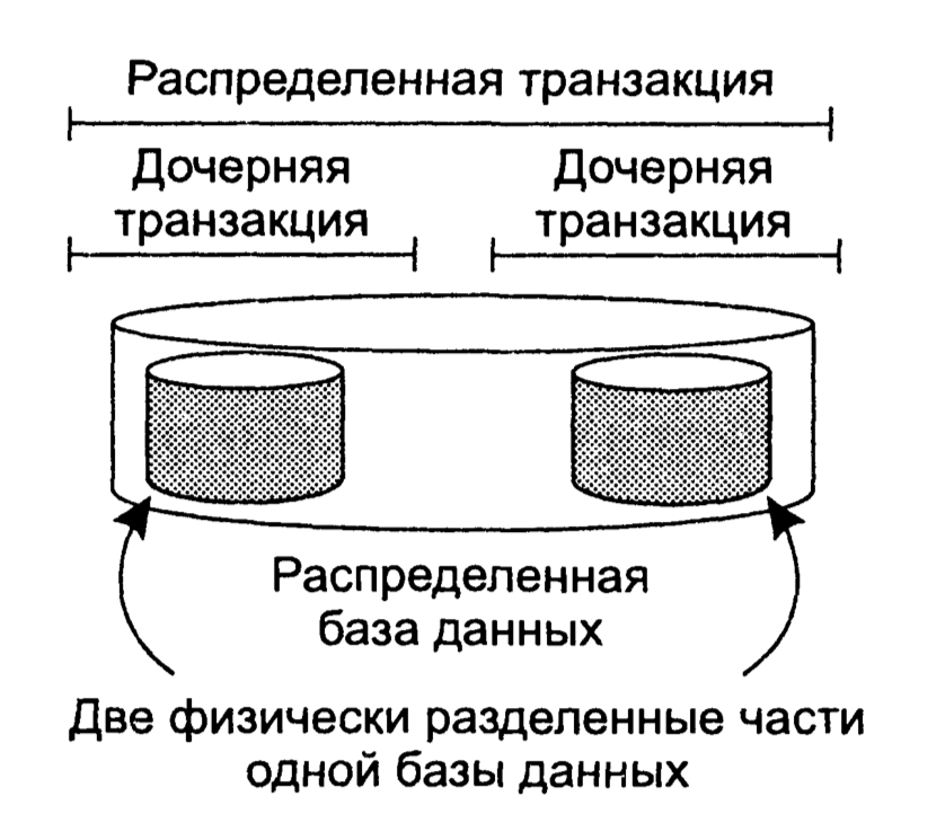
\includegraphics[width=0.8\textwidth]{assets/distributed/Transaction.png}
    \caption{Понятие распределенной транзакции}
\end{figure}

\subsubsection{Модель обработки транзакций}

Распределенная транзакция выполняет операции над данными, расположенными на нескольких сетевых узлах (серверах) одновременно. 
В распределенных СУБД обработка транзакций значительно усложняется, так как требуется обеспечить согласованность изменений на 
разных географически удаленных узлах базы данных, обеспечить атомарность и гарантировать целостность данных даже в случае сетевых 
сбоев или отказов отдельных серверов \autocite[гл. Введение]{Tanenbaum}.

Для обеспечения выполнения этих требований распределенные СУБД используют протоколы фиксации, которые будут описаны далее в разделе 
"Протоколы фиксации". Эти протоколы позволяет всем серверам, участвующим в транзакции, либо совместно подтвердить (зафиксировать), 
либо совместно отказаться (откатить) от ее выполнения. Такой подход позволяет сохранить принцип атомарности и согласованности транзакции 
вне зависимости от условий физического размещения данных и особенностей сетевой инфраструктуры.

Подробности об основных принципах обработки транзакций, журналирования, операциях фиксации и отката в контексте СУБД можно посмотреть 
в разделах «Механизмы обеспечения целостности СУБД» и "Механизмы, поддерживающие высокую готовность".

\subsubsection{Мониторы обработки транзакций}~\\

Мониторы обработки транзакций (Transaction Processing Monitor - TPM) — специализированное промежуточное программное обеспечение (middleware), 
обеспечивающее выполнение распределенных транзакций. TPM координируют работу нескольких серверов баз данных, гарантируя соблюдение ACID-свойств 
(атомарность, согласованность, изолированность, долговечность) для распределенных транзакций \autocite{TransactionMonitors}.

Архитектура приложений, использующих монитор обработки транзакций, состоит из трех частей \autocite{TPM}.

\begin{itemize}
    \item Уровень графического интерфейса - находится на компьютере клиента.
    \item Прикладной уровень - находится на множестве отдельных серверов приложений.
    \item Уровень данных - находится на отдельных серверах баз данных.
\end{itemize}

\begin{figure}[h!]
    \centering
    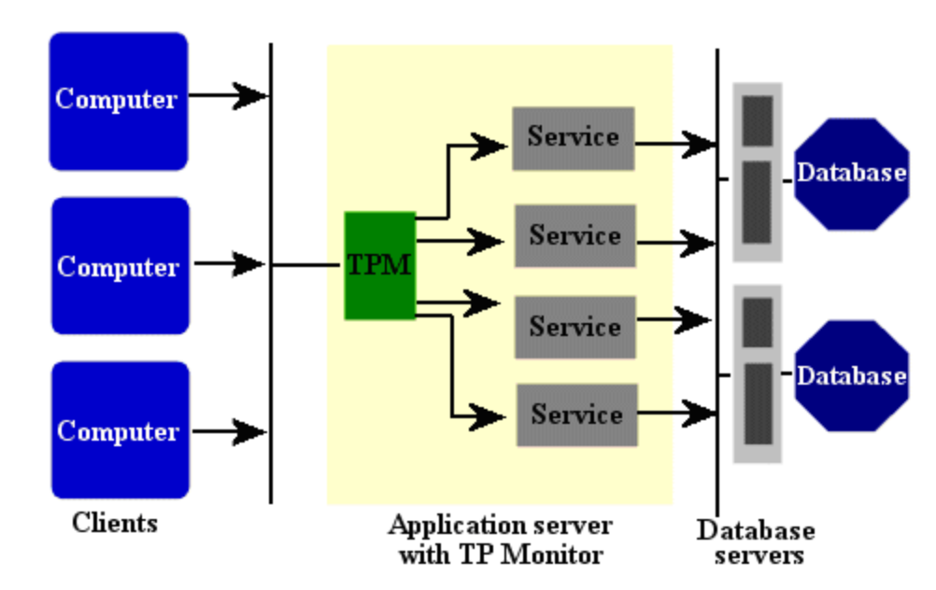
\includegraphics[width=0.8\textwidth]{assets/distributed/TPM.png}
    \caption{Архитектура приложений, использующих TPM}
\end{figure}

Архитектура системы обработки транзакций: 

\begin{itemize} 
    \item Прикладная программа — определяет границы транзакций, устанавливает конкретные действия, которые будет выполнять транзакция, и контролирует операции с данными, вызывая менеджеры ресурсов. 
    \item Менеджеры ресурсов — обеспечивают доступ к общим ресурсам, таким как базы данных, системы очередей сообщений и другие компоненты распределенной системы. 
    \item Менеджер транзакций — отвечает за создание транзакций, мониторинг их выполнения и координацию успешного завершения или отката при возникновении ошибок. 
\end{itemize}

Процесс обработки распределенной транзакции включает следующие шаги (рис. \ref{tpm_process}):

\begin{itemize}
    \item Клиент инициирует транзакцию, обращаясь к TPM, который генерирует идентификатор транзакции и создает контекст транзакции.
    \item Клиент взаимодействует с серверами ресурсов через удаленные вызовы процедур (RPC), передавая в каждом запросе контекст транзакции.
    \item Сервер извлекает контекст, регистрируется в TPM как участник транзакции и обрабатывает запрос.
    \item По завершении всех операций клиент уведомляет TPM о необходимости фиксации или отката транзакции.
    \item TPM координирует двухфазный протокол фиксации (2PC) между всеми участвующими серверами, обеспечивая атомарность транзакции \autocite{WebServices}.
(Рис. \ref{tpm_process}). 
\end{itemize}

\begin{figure}[h!]
    \centering
    \includegraphics[width=0.8\textwidth]{assets/distributed/TPM_arch.png}
    \caption{Процесс взаимодействия с TPM}
    \label{tpm_process}
\end{figure}

Примеры мониторов транзакций:
\begin{itemize}
  \item CICS (Система управления информацией о клиентах) для мэйнфреймов IBM;
  \item IBM Information Management System (IMS, точнее, её компонент IMS TM, также известный как IMS DC);
  \item ACMS (система управления приложениями) для OpenVMS;
  \item UNIVAC TIP;
  \item Transarc Encina;
  \item Oracle Tuxedo
\end{itemize}


\subsubsection{Корпоративная среда обработки транзакций}~\\

В этом разделе мы используем терминологию, предложенную автором статьи \autocite{TransactionMonitors}.

Корпоративная среда обработки транзакций  (Enterprise Transaction Processing — ETP) представляет собой комплексную инфраструктуру для выполнения распределенных транзакций в масштабах 
предприятия. Архитектура ETP строится на трех уровнях компьютерных систем \autocite{TransactionMonitors}:

\begin{itemize}
    \item Ряд 1: Персональные станции - рабочие станции пользователей, обеспечивающие интерфейс взаимодействия с системой;
    \item Ряд 2: Компьютеры под управлением ОС UNIX, на которых функционирует ядро TPM, и, как правило, реляционные СУБД, выступающие в качестве менеджера ресурсов;
    \item Ряд 3: Mainframe-системы или компьютеры под управлением UNIX c RISC-архитектурой процессоров;
\end{itemize}

Таким образом, среда обработки транзакций формируется из набора разнородных компьютеров (и соответствующих ОС),
ранжируемых от персональных компьютеров до мэйнфрейм-систем. TPM на базе UNIX представляет собой своего
рода "клей", который связывает вместе компьютеры трех рядов в открытую унифицированную среду обработки транзакций.

\begin{figure}[h!]
    \centering
    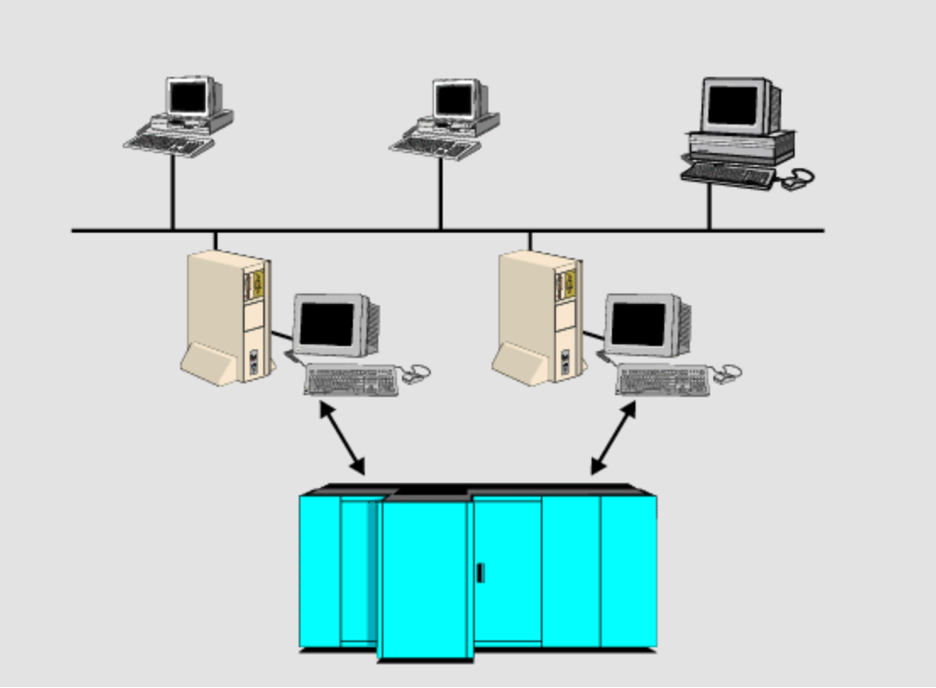
\includegraphics[width=0.8\textwidth]{assets/distributed/ETP.png}
    \caption{Промышленная среда обработки транзакций}
\end{figure}

При этом трехуровневая архитектура ETP характерна преимущественно для организаций, где исторически используются мэйнфреймы(типично для Европы 
и США). Для российских - более характерна двухуровневая архитектура ETP, включающая только клиентский уровень и серверы приложений/БД. При 
этом следует различать трехзвенную модель "клиент-сервер" (см. раздел 6.1 "Распределенные вычислительные среды"), относящуюся к логической 
организации, и архитектуру ETP, описывающую физическое распределение вычислительных ресурсов.

Ключом к интеграции систем, функционирующих на компьютерах различных рядов, является специализированный
интерфейс прикладного программирования ATMI (Application Transaction Manager Interface), обеспечивающий \autocite{TransactionMonitors}:
\begin{itemize}
    \item для ряда 1 - формирование и передачу запросов от клиентов к серверам, выполняющимся на компьютерах ряда 2
    \item для ряда 2 - обработку запросов, поступающих от компьютера ряда 1 (в том числе и с
    обращением к менеджеру ресурсов), и, по необходимости, формирование и направление
    запросов к серверам, выполняющимся на компьютерах ряда 3
    \item для ряда 3 - обработку запросов, поступающих от серверов ряда 2
\end{itemize}

\subsection{Протоколы фиксации}

Протоколы фиксации транзакций представляют собой механизм, обеспечивающий атомарность 
выполнения транзакций в распределенных базах данных. Их основная задача — гарантировать, что все участвующие в 
транзакции узлы либо зафиксируют изменения, либо откатят их, даже при возникновении сетевых сбоев или отказе отдельных 
компонентов системы. \autocite{FixProtocols}

Распределенная транзакция имеет дело с разделяемыми данными на нескольких географически рассредоточенных серверах. 
На заключительном этапе каждый сервер должен выполнить некоторое количество завершающих операций, предписанных транзакцией. 
На этой стадии все серверы, невзирая на отказы, должны согласовать окончательное решение — транзакция должна быть фиксирована 
или прервана. Даже одного голоса, поданного за прерывание транзакции, достаточно для того, чтобы транзакция была прервана.
 Какое бы решение ни было принято, оно должно быть передано всем участникам транзакции. 
 
Условия задачи атомарного завершения (commitment):

\begin{itemize}
    \item Согласие (Agreement). Все процессы принимают одно и то же решение.
    \item Валидность (Validity). Если один из процессов голосует за прерывание, тогда транзакция должна быть прервана. 
    Если все процессы голосуют за фиксацию, и отказы отсутствуют, тогда транзакция должна быть фиксирована.
    \item Завершение (Termination). Все корректно работающие процессы должны в конечном счете прийти к финальному 
    решению.
\end{itemize}

Протоколы фиксации спроектированы так, чтобы работать в асинхронной системе, в которой серверы могут отказывать и сообщения 
могут теряться. Свойство согласия подразумевает, что все серверы достигают одного и того же решения \autocite{Fix}.

\subsubsection{Распределенная однофазная фиксация}

Распределенная однофазная фиксация (Distributed One-Phase Commit, 1PC) представляет собой упрощенный протокол 
атомарной фиксации транзакций в распределенных базах данных, требующий всего одного раунда обмена сообщениями 
между координатором и участниками.

Начиная транзакцию, клиентское приложение делает запрос одному из процессов службы поддержки транзакций на ближайшем 
доступном сервере. Этот процесс становится координатором транзакции. Другие серверы, вовлеченные в эту транзакцию,
называются участниками транзакции.

Координатор распределяет работу по осуществлению транзакции между участниками и на заключительном этапе посылает 
сообщение фиксация (COMMIT) или прерывание (ABORT) всем участникам транзакции и ждет, пока все они пришлют подтверждения 
о том, что распоряжение выполнено. Это так называемая однофазная фиксация. При этом не исключено, что вследствие локальных 
проблем (подобных отказу компонентов или конфликтам параллельного исполнения) некоторые участники не смогут проинформировать
 о своем решении координатора и других участников. Поскольку решение должно быть принято в течение одной фазы, координатор и 
 корректные участники, не будучи оповещенными о проблемах других участников, не смогут прийти к согласию относительно возможности
фиксации или прерывания транзакции. Для практического применения необходима более сложная схема \autocite{Fix}.

\subsubsection{Распределенная двухфазная фиксация}

Протокол двухфазной фиксации (Two-phase Commit Protocol, 2РС) был спроектирован, чтобы преодолеть ограничения протокола
однофазной фиксации. В течение первой фазы координатор посылает сообщение VOTE каждому участнику, спрашивая у них, намерены 
ли они фиксировать транзакцию или прерывать ее. Далее координатор анализирует собранные ответы.

Если все серверы готовы фиксировать транзакцию, тогда в течение второй фазы координатор посылает всем участникам сообщение COMMIT. 
В противном случае, если по крайней мере один из участников проголосовал за прерывание, координатор посылает всем участникам сообщение ABORT.

Каждый участник после посылки своего голоса ждет получения сообщения (COMMIT или ABORT) от координатора. После получения сообщения каждый 
участник локально выполняет необходимые действия по фиксации или прерыванию транзакции. Очевидно, что условия согласия, валидности и 
завершения выполняются, и следовательно, протокол двухфазного подтверждения решает задачу распределенной фиксации транзакции \autocite{Fix}.

\textbf{Обработка ошибок}

Протокол 2РС может попасть в трудную ситуацию в случае сбоя. Например, один из участников может отказать из-за поломки и, следовательно, не ответить. 
Сообщения также могут быть потеряны. Это делает реализацию протокола двухфазной фиксации нетривиальной. В варианте чисто асинхронного исполнения, 
когда координатор или участник блокируются в ожидании сообщения, они не смогут узнать, что произошло: поломка сервера, потеря или задержка сообщения. 

На практике для обнаружения потерь и отказов процессов часто используют таймауты, но это не считается надежным решением. Поэтому в случае любого сомнения 
систему принято возвращать к безопасной конфигурации путем прерывания всех транзакций. Некоторые варианты отказов и способы борьбы с ними суммированы ниже.

Вариант 1. Если (на фазе 1) координатор не получает ответа по крайней мере от одного участника в период таймаута, тогда он решает прервать транзакцию и 
рассылает всем участникам сообщение ABORT.

Вариант 2. Если (на фазе 1) участник не получает сообщения VOTE от координатора в течение определенного таймаута, предполагая, что координатор отказал или 
сообщение VOTE потеряно или задержано, он посылает сообщение ABORT координатору и затем локально прерывает транзакцию.

Вариант 3. Если (на фазе 2) участник не получает сообщение COMMIT или ABORT от координатора в течение оговоренного периода времени (это может быть случай 
поломки координатора после посылки сообщений ABORT или COMMIT только части серверов), тогда он остается в состоянии неопределенности до тех пор, пока 
координатор не восстановится и не реинсталлируется в системе. При этом на неопределенный период ресурсы могут оставаться заблокированными, мешая другим 
транзакциям. По этой причине протокол 2РС также называют протоколом блокирующего подтверждения. Блокировка ресурсов — один из недостатков протокола 
двухфазной фиксации \autocite{Fix}.

\subsubsection{Распределенная трехфазная фиксация}

Протокол трёхфазной фиксации (3PC) — это расширение протокола двухфазной фиксации (2PC), которое позволяет избежать проблемы блокировки при определённых условиях. В частности, 
предполагается, что не происходит разделения сети на части и не более k узлов выходят из строя, где «k» — заранее заданное число. При соблюдении упомянутых условий протокол позволяет 
избежать блокировки за счёт введения дополнительной третьей фазы, в которой в принятии решения о фиксации участвуют несколько узлов.

Вместо того чтобы напрямую сохранять решение о фиксации в постоянном хранилище, координатор сначала гарантирует, что по крайней мере «k» других узлов знают, что он намерен зафиксировать 
транзакцию.

В ситуации, когда координатор выходит из строя, оставшиеся узлы должны сначала выбрать нового координатора. Этот новый координатор проверяет состояние протокола на оставшихся узлах. 
Если координатор решил зафиксировать транзакцию, то по крайней мере один из других «k» узлов, о которых он сообщил, будет работать и обеспечит соблюдение решения о фиксации транзакции. 
Новый координатор перезапускает третью фазу протокола, если какой-либо из оставшихся узлов знал, что старый координатор намеревался зафиксировать транзакцию. В противном случае новый 
координатор прерывает транзакцию.

При опросе участников, если он обнаруживает, что некоторые узлы находятся на этапе фиксации, он предполагает, что предыдущий координатор перед сбоем принял решение о фиксации.
Следовательно, он может завершить протокол фиксацией. Аналогичным образом, если участник отвечает, что он не получил команду на подготовку к фиксации, то новый координатор может 
предположить, что предыдущий координатор потерпел неудачу ещё до того, как начал подготовку к фиксации. Следовательно, он может с уверенностью предположить, что ни один другой участник 
не зафиксировал изменения, и поэтому он может безопасно прервать транзакцию \autocite{3PC}.

Разницу между трёхфазным и двухфазным протоколами фиксации можно понять по рисункам \ref{2pc} и \ref{3pc}.

\begin{figure}[h!]
    \centering
    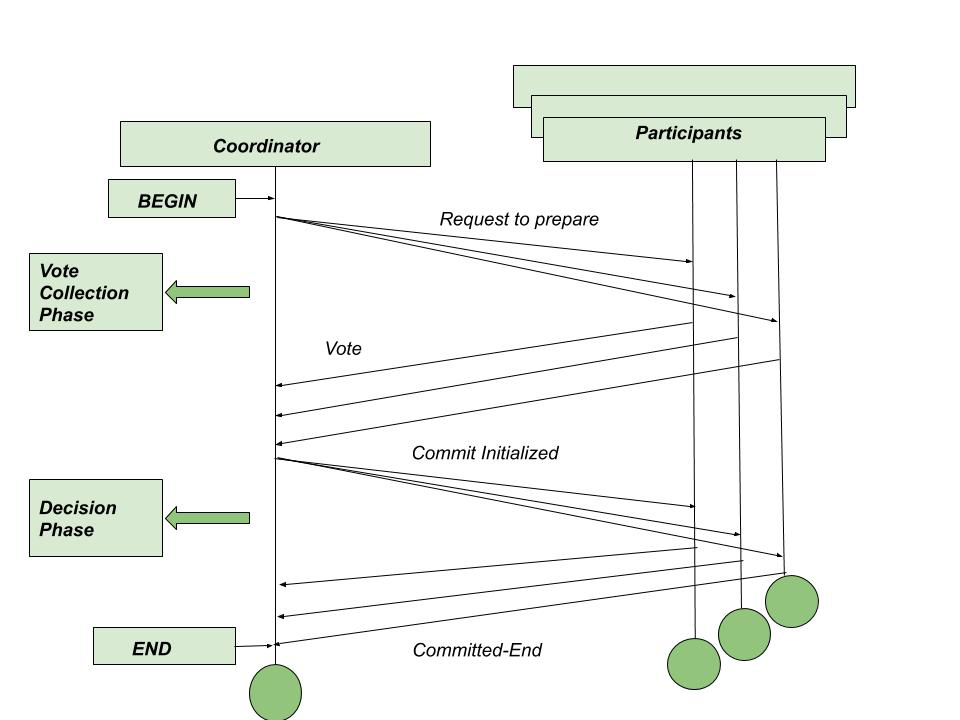
\includegraphics[width=0.8\textwidth]{assets/distributed/2PhaseCommit.png}
    \caption{Протокол двухфазной фиксации}
    \label{2pc}
\end{figure}

\begin{figure}[h!]
    \centering
    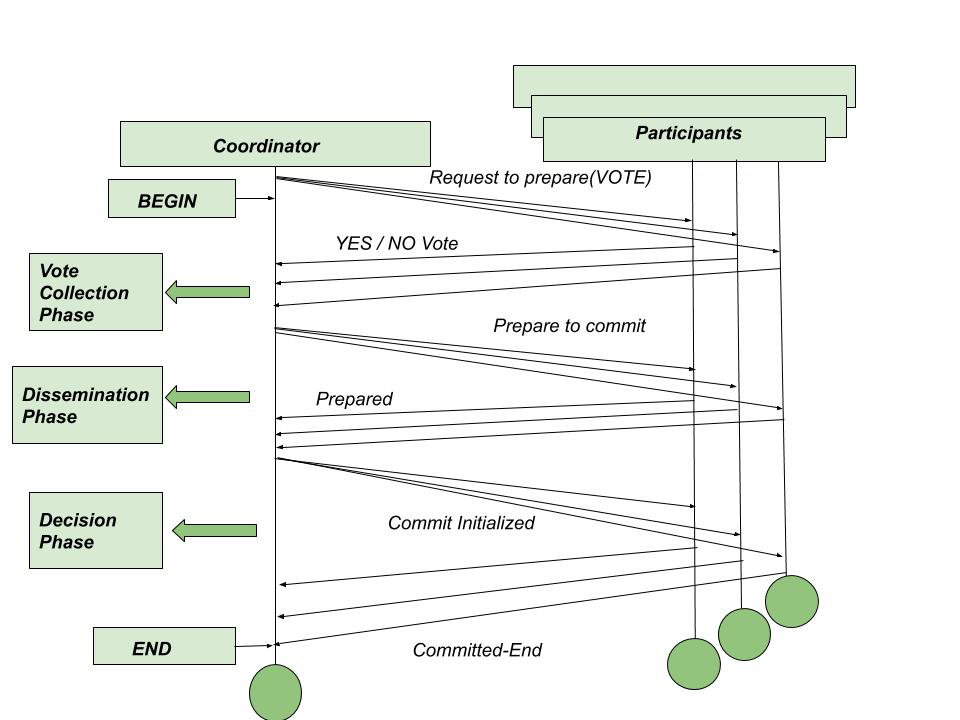
\includegraphics[width=0.8\textwidth]{assets/distributed/3PhaseCommit.png}
    \caption{Протокол трехфазной фиксации}
    \label{3pc}
\end{figure}

Таким образом, между фазами запроса на фиксацию и окончательной фиксацией в отличие от 2PC добавляется фаза предварительной фиксации:

\begin{itemize}
    \item Координатор отправляет всем участникам сообщение \texttt{prepare to commit}
    \item Участники выполняют все необходимые операции для подготовки к окончательной фиксации
    \item Участники переходят в состояние "готов к фиксации"
    \item Каждый участник отправляет координатору подтверждение о готовности (\texttt{ACK})
\end{itemize}

\subsubsection{Защищенные протоколы фиксации}

Некоторые примеры с ссылками на описание проткоолов:

\begin{itemize}
    \item BFT-2PC \autocite{BFT-2PC}
    \item PBFT \autocite{PBFT}
    \item PoW (Proof of Work Commit) \autocite{PoS_PoW}
    \item PoS (Proof of Stake Commit) \autocite{PoS_PoW}
\end{itemize}

\paragraph{Обработка распределенных транзакций в базах данных с многоуровневой секретностью (MLS)}~\\

Для внедрения разграничения доступа в системы  управления  базами  данных  (СУБД  -
DBMS)  предложены некоторые решения. Однако эти решения не достаточно
эффективны, поэтому рассмотрим понятие  системы
управления  базами  данных  с  многоуровневым  разграничением доступа (MLS/DBMS).

Известно, что в MLS/DBMS не ко всем данным, содержащимся в  базе
данных, доступ осуществляется одинаково. Однако современные СУБД, как
правило,  не имеют адекватных средств диагностики и механизма определения
того, что пользователь имеет возможность доступа только  к  тем
данным,  которые являются релевантными. Таким образом, MLS/DBMS отличается
от соответствующих DBMS,  по крайней  мере,  следующими  двумя
особенностями \autocite{SecureFix}:
\begin{itemize}
    \item каждый элемент данных в базе данных связан с уровнем доступа
    \item доступ пользователя к данным должен контролироваться релевантностью для данного пользователя
\end{itemize}
Разработка сервиса MLS/DBMS в современных компьютерных  системах
представляет  много  проблем. До настоящего времени внедрение многоуровневого
разграничения доступа в операционную  систему  представляет
собой  значительные трудности. Решение этой проблемы в виде аббревиатуры
обозначается ТСВ. Хотя в разрешении вопросов ТСВ  для  удаленных
пользователей  в  MLS/DBMS вводятся компромиссы, остается много проблем,
которые требуется разрешать. Наиболее очевидная проблема состоит
в том, что вопросы классификации в СУБД значительно  сложнее,  чем  в
файловых  системах  и могут быть сложнее реализованы. Другая проблема
состоит в том, что для классификации данных,  содержащих  контекстные
представления,  временные параметры, их композицию, необходимы унифицированные базы данных 

Подробнее можно почитать в \autocite{SecureFix}.

\subsubsection{Алгоритмы консенсуса}

\paragraph{Проблема консенсуса в распределённых системах}

\textbf{Проблема консенсуса} — фундаментальная задача распределённых систем, требующая согласования общего решения между узлами в условиях возможных сбоев, задержек сообщений или 
неисправностей участников. Формально, каждый узел системы предлагает своё начальное значение, и все корректные узлы должны прийти к единому решению, удовлетворяющему следующим условиям \autocite{Consensus}: 

\begin{itemize} 
    \item \textbf{Согласованность (Agreement)}: Все узлы принимают одно и то же значение. 
    \item \textbf{Целостность (Integrity)}: Решение должно быть предложено хотя бы одним узлом. 
    \item \textbf{Завершаемость (Termination)}: Каждый корректный узел в конечном итоге принимает решение. 
\end{itemize}

\paragraph{Теоретические ограничения} 

В распределённых системах достижение консенсуса осложнено теоретическими ограничениями: 

\begin{itemize} 
    \item \textbf{Теорема FLP} (Фischer, Lynch, Paterson, 1985): В асинхронной системе с хотя бы одним отказом узла консенсус невозможен, если возможна произвольная задержка сообщений \autocite{Fischer1985}. 
    \item \textbf{CAP-теорема} (Brewer, 2000): Система может гарантировать только два из трёх свойств: согласованность (Consistency), доступность (Availability), устойчивость к разделению (Partition tolerance) \autocite{Brewer2012}. 
\end{itemize}

\paragraph{Типы отказов} 

Алгоритмы консенсуса классифицируются по типу отказов, которые они могут преодолеть: 

\begin{itemize} 
    \item \textbf{Аварийные отказы (Crash faults)}: Узел перестаёт отвечать, но не действует злонамеренно. 
    \item \textbf{Византийские отказы (Byzantine faults)}: Узел может произвольно искажать данные или нарушать протокол \autocite{Castro1999}. 
\end{itemize}


\subsection{Тиражирование данных}

\textbf{Тиражирование данных} - это асинхронный перенос изменений объектов исходной базы данных (source database)
в базы данных, принадлежащие к различным узлам распределенной системы. Тиражирование данных может происходит
двумя различными способами: \textbf{шардингом} (или, иначе говоря, шардированием, фрагментацией) и \textbf{репликацией}.

\subsubsection{Шардинг (sharding)}

\textbf{Шардинг} — это метод проектирования базы данных, при котором данные разделяются на группы и хранятся на разных серверах. Это улучшает производительность, поскольку данные хранятся там, где они чаще всего используются, что уменьшает сетевой трафик.

Существуют два основных вида шардирования: \textbf{горизонтальное} и \textbf{вертикальное}. Они соответствуют операциям сокращения и проекции в реляционных базах данных. Важно, чтобы все фрагменты были независимыми, то есть ни один из фрагментов не может быть представлен как производный от других фрагментов.

Одной из ключевых особенностей шардинга является поддержка независимости от шардирования. Это означает, что пользователи могут работать так, как если бы данные в действительности были вовсе не шардированы. Это упрощает разработку пользовательских программ и выполнение терминальных операций.

Если обеспечивается независимость от шардирования, пользователи получают данные в виде представления, в котором шарды логически скомбинированы с помощью операций соединения и объединения. Задачей системного оптимизатора является определение шардов, к которым требуется доступ для выполнения запросов пользователя.
\autocite{IntroBD2014}

\paragraph{Алгоритмы шардинга} ~\\
Ранее уже упоминалось о двух основных вида шардинга: \textit{горизонтальный} и \textit{вертикальный}. Стоит их разобрать по подробнее и
рассказать и про другие виды шардирования, такие как шадинг на основе каталогов и шардинг на основе ключей.

\paragraph{Горизонтальное шардирование} ~\\
В этом методе мы разбиваем данные на основе диапазонов заданного значения, присущего каждой сущности. Допустим, у вас
есть база данных имен ваших онлайн-клиентов и информации об электронной почте. Вы можете разделить эту информацию на
два осколка. В одном осколке вы можете хранить информацию о клиентах, чье имя начинается с A-P, а в другом - информацию
об остальных клиентах.

\begin{figure}[H]
    \centering
    \includegraphics[width=100mm]{assets/distributed/Horizontal-Sharding}
    \caption{Горизонтальное шардирование}
    \label{fig:Horizontal-Sharding}
\end{figure}

\textbf{Горизонтальное шардирование} - самый простой метод сегментирования для реализации. Каждый осколок содержит
другой набор данных, но все они имеют ту же схему, что и исходная база данных. В этом методе вам просто нужно
определить, в какой диапазон попадают ваши данные, а затем вы можете сохранить запись в соответствующий шард. Этот
метод лучше всего подходит для хранения нестатических данных (например, хранение контактной информации студентов
колледжа).

Недостатком этого метода является то, что данные могут быть неравномерно распределены по шардам. В приведенном выше
примере у вас может быть много клиентов, имена которых попадают в категорию A-P. В таких случаях первый осколок должен
будет взять на себя больше нагрузки, чем второй, и это может стать узким местом системы. \autocite{DatabaseSharding}

\paragraph{Вертикальное шардирование} ~\\
В этом методе мы разделяем весь столбец из таблицы и помещаем эти столбцы в новые отдельные таблицы. Данные полностью
независимы от одного раздела к другому. Кроме того, каждый раздел содержит как отдельные строки, так и столбцы. Возьмем,
к примеру, функции Twitter. Мы можем разделить различные функции объекта на разные сегменты на разных машинах. В
Твиттере у пользователя может быть профиль, количество подписчиков и некоторые твиты, опубликованные им самим. Мы можем
разместить профили пользователей на одном осколке, подписчиков - на втором, а твиты - на третьем.

\begin{figure}[H]
    \centering
    \includegraphics[width=100mm]{assets/distributed/Vertical-Sharding}
    \caption{Вертикальное шардирование}
    \label{fig:Vertical-Sharding}
\end{figure}

В этом методе вы можете отделить и обработать критическую часть (например, профили пользователей) от некритической части
ваших данных (например, сообщения в блоге) по отдельности и построить вокруг нее различные модели репликации и
согласованности. Это одно из главных преимуществ этого метода.

Основным недостатком этой схемы является то, что для ответа на некоторые запросы вам, возможно, придется комбинировать
данные из разных шардов, что неоправданно увеличивает сложность разработки и эксплуатации системы. Кроме того, если
ваше приложение будет расти позже, и вы добавите в него еще несколько функций, вам придется дополнительно сегментировать
базу данных с конкретными функциями на нескольких серверах. \autocite{DatabaseSharding}

\paragraph{Шардинг на основе каталогов} ~\\
В этом методе мы создаем и поддерживаем службу поиска или таблицу поиска для исходной базы данных. В основном мы
используем ключ осколка для таблицы поиска и делаем сопоставление для каждого объекта, существующего в базе данных.
Таким образом, мы отслеживаем, какие осколки базы данных содержат какие данные.

Таблица поиска содержит статический набор информации о том, где можно найти конкретные данные. На приведенном выше
изображении вы можете видеть, что мы использовали зону доставки в качестве ключа осколка. Во-первых, клиентское
приложение запрашивает службу поиска, чтобы узнать осколок (раздел базы данных), на котором размещены данные. Когда
служба поиска возвращает осколок, она запрашивает/обновляет этот осколок.

\begin{figure}[H]
    \centering
    \includegraphics[width=100mm]{assets/distributed/Directory-Based-Sharding}
    \caption{Шардинг на основе каталогов}
    \label{fig:Directory-Based-Sharding}
\end{figure}

Сегментация на основе каталогов гораздо более гибкая, чем сегментация на основе диапазонов и ключей. В сегменте на
основе диапазонов вы обязаны указать диапазоны значений. В key-based вы обязаны использовать фиксированную хэш-функцию,
которую трудно изменить позже. При таком подходе вы можете использовать любой алгоритм, который хотите назначить для
записей данных в сегменты. Кроме того, при таком подходе легко динамически добавлять шарды.

Основным недостатком этого подхода является единственная точка отказа таблицы поиска. Если он будет поврежден или не
удался, это повлияет на запись новых данных или доступ к существующим данным из таблицы. \autocite{DatabaseSharding}

\paragraph{Шардинг на основе ключей} ~\\
Этот метод также известен как сегментация на основе хэша. Здесь мы берем значение объекта, такого как идентификатор
клиента, адрес электронной почты клиента, IP-адрес клиента, почтовый индекс и т. д., и мы используем это значение в
качестве входных данных хэш-функции. Этот процесс генерирует хэш-значение, которое используется для определения того,
какой шард нам нужно использовать для хранения данных. Мы должны иметь в виду, что значения, введенные в хэш-функцию,
должны поступать из одного и того же столбца (ключ осколка), чтобы данные размещались в правильном порядке и
согласованно. В принципе, ключи осколков действуют как первичный ключ или уникальный идентификатор для отдельных строк.

\begin{figure}[H]
    \centering
    \includegraphics[width=100mm]{assets/distributed/Keybased-Sharding}
    \caption{Шардинг на основе ключей}
    \label{fig:Keybased-Sharding}
\end{figure}

Рассмотрим пример, что у вас есть 3 сервера баз данных, и каждый запрос имеет идентификатор приложения, который
увеличивается на 1 каждый раз, когда регистрируется новое приложение. Чтобы определить, на каком сервере должны быть
размещены данные, мы выполняем операцию по модулю для этих приложений id с номером 3. Затем остаток используется для
идентификации сервера для хранения наших данных.

Недостатком этого метода является эластичная балансировка нагрузки, что означает, если вы попытаетесь динамически
добавлять или удалять серверы баз данных, это будет сложный и дорогостоящий процесс. Например, в приведенном выше
примере, если вы добавите еще 5 серверов, вам нужно добавить больше соответствующих хэш-значений для дополнительных
записей. Кроме того, большинство существующих ключей необходимо переназначить на их новое, правильное хэш-значение,
а затем перенести на новый сервер. Хэш-функция должна быть изменена с модуля 3 на модуль 8. В то время как миграция
данных действует, как новые, так и старые хэш-функции не будут действительны. Во время миграции ваше приложение не
сможет обслуживать большое количество запросов, и вы будете испытывать простои для своего приложения до завершения
миграции. \autocite{DatabaseSharding}

\paragraph{Географический шардинг} ~\\
Шардирование по географическому признаку позволяет хранить определенные данные вблизи своих потребителей и
удовлетворять нормативным требованиям, когда данные должны находиться в определенной юрисдикции. Однако данный способ
шардирования не является самодостаточным: шарды могут быть загружены не равномерно, и отличие может быть на порядки.
На пример, экземпляр базы данных, хранящий данные пользователей Москвы и Московской области, будет намного превышать
другой экземпляр базы данных, который хранит информацию о пользователях из Владимира. Таким образом, недостатком
данного метода является необходимость дополнительного использования других методов шардирования.

\subsubsection{Репликация} ~\\

\textbf{Репликация} — это процесс изменения одного набора данных, называемого репликой, в ответ на изменения другого
набора данных, называемого основным. Репликация желательна по крайней мере по двум причинам. Во-первых, она способна
обеспечить более высокую производительность, поскольку приложения смогут обрабатывать локальные копии вместо того,
чтобы устанавливать связь с удаленными узлами. Во-вторых, наличие репликации может также обеспечивать более высокую
степень доступности, поскольку любой реплицируемый объект остается доступным для обработки (по крайней мере, для выборки
данных), пока хотя бы одна реплика в системе остается доступной. Главным недостатком репликации, безусловно, является
то, что если реплицируемый объект обновляется, то и все его копии должны быть обновлены (проблема распространения
обновлений).

Очевидно, что репликация, как и шардирование, теоретически должна быть "прозрачной для пользователя". Другими словами,
система, которая поддерживает репликацию данных, должна также поддерживать независимость от репликации (иногда говорят
"прозрачность репликации"). Для пользователей должна быть создана такая среда, чтобы они, по крайней мере, с логической
точки зрения могли считать, что в действительности данные не дублируются. Независимость от репликации (как и
независимость от шардирования) является весьма желательной, поскольку она упрощает создание пользовательских программ и
выполнение терминальных операций. В частности, независимость от репликации позволяет создавать и уничтожать дубликаты в
любой момент в соответствии с изменяющимися требованиями, не затрагивая при этом никакие из пользовательских программ
или терминальных операций.

Из требования независимости от репликации следует, что к обязанностям системного оптимизатора также относится
определение, какой именно из физических дубликатов будет применен для доступа к данным при выполнении каждого
введенного пользователем запроса. \autocite{IntroBD2014}

Можно выделить три \textbf{подхода к репликации}:
\begin{itemize}
    \item Блочная репликация на уровне системы хранения данных;
    \item Физическая репликация на уровне СУБД;
    \item Логическая репликация на уровне СУБД.
\end{itemize}

\paragraph{Блочная репликация} ~\\
При блочной репликации каждая операция записи выполняется не только на основном диске, но и на резервном. Таким образом
тому на одном массиве соответствует зеркальный том на другом массиве, с точностью до байта повторяющий основной том.

К достоинствам такой репликации можно отнести простоту настройки и надёжность. Записывать данные на удалённый диск может
либо дисковый массив, либо нечто (устройство или программное обеспечение), стоящее между хостом и диском. Если дисковый
массив не способен реплицировать данные, между хостом и массивом может быть установлен агент, осуществляющей запись на
два массива сразу. Агент может быть как отдельным устройством, так и программным компонентом. В отличие от дискового
массива, который может работать только с таким же массивом или, как минимум, с массивом того же производителя, агент
может работать с совершенно разными дисковыми устройствами.

Главное назначение блочной репликации – обеспечение отказоустойчивости. Если база данных потеряна, то можно
перезапустить её с использованием зеркального тома. Блочная репликация хороша своей универсальностью, но за
универсальность приходится платить.

Во-первых, никакой сервер не может работать с зеркальным томом, поскольку его операционная система не может управлять
записью на него; с точки зрения наблюдателя данные на зеркальном томе появляются сами собой. В случае аварии (отказ
основного сервера или всего ЦОДа, где находится основной сервер) следует остановить репликацию, размонтировать основной
том и смонтировать зеркальный том. Как только появится возможность, следует перезапустить репликацию в обратном
направлении.

Во-вторых, сама СУБД на резервном сервере может быть запущена только после монтирования диска. В некоторых операционных
системах, например, в Solaris, память под кеш при выделении размечается, и время разметки пропорционально объёму
выделяемой памяти, то есть старт экземпляра будет отнюдь не мгновенным. Плюс ко всему кеш после рестарта будет пуст.

В-третьих, после запуска на резервном сервере СУБД обнаружит, что данные на диске неконсистентны, и нужно потратить
значительное время на восстановление с применением журналов повторного выполнения: сначала повторить те транзакции,
результаты которых сохранились в журнале, но не успели сохраниться в файлы данных, а потом откатить транзакции, которые
к моменту сбоя не успели завершиться. \autocite{Replication}

\paragraph{Физическая репликация (master-slave)} ~\\
Журналы (redo log или write-ahead log) содержат все изменения, которые вносятся в файлы базы данных. Идея физической
репликации состоит в том, что изменения из журналов повторно выполняются в другой базе (реплике), и таким образом данные
в реплике повторяют данные в основной базе байт-в-байт \autocite{PhysLogPeplic}.

Журналы СУБД не предназначены для использования вне этой платформы, их формат не документируется и может меняться без
предупреждения. Отсюда совершенно естественное требование, что физическая репликация возможна только между экземплярами
одной и той же версии одной той же СУБД. Отсюда же возможные ограничения на операционную систему и архитектуру
процессора, которые тоже могут влиять на формат журнала.

Естественно, никаких ограничений на модели СХД физическая репликация не накладывает. Более того, файлы в базе-реплике
могут располагаться совсем по-другому, чем на базе-источнике – надо лишь описать соответствие между томами, на которых
лежат эти файлы.

Запись данных в реплику невозможна, поскольку изменения в неё приходят побайтно, и реплика не может обеспечить
конкурентное исполнение своих запросов. В случае повреждения файла в основной базе можно просто скопировать
соответствующий файл с реплики. Однако стоит учесть, что файл на реплике может быть не идентичен файлу в основной базе:
когда файл расширяется, новые блоки в целях ускорения ничем не заполняются, и их содержимое случайно. База может
использовать не всё пространство блока (например, в блоке может оставаться свободное место), но содержимое
использованного пространства совпадает с точностью до байта \autocite{PhysLogPeplic}.

Физическая репликация может быть как синхронной, так и асинхронной. При асинхронной репликации всегда есть некий набор
транзакций, которые завершены на основной базе, но ещё не дошли до резервной, и в случае перехода на резервную базу при
сбое основной эти транзакции будут потеряны. При синхронной репликации завершение операции commit означает, что все
журнальные записи, относящиеся к данной транзакции, переданы на реплику. Важно понимать, что получение репликой журнала
не означает применения изменений к данным. При потере основной базы транзакции не будут потеряны, но если приложение
пишет данные в основную базу и считывает их из реплики, то у него есть шанс получить старую версию этих данных \autocite{PhysLogPeplic}.

Физическая репликация базы данных имеет множество преимуществ перед репликацией средствами СХД \autocite{PhysLogPeplic}:
\begin{itemize}
    \item объём передаваемых данных меньше за счёт того, что передаются только журналы, но не файлы с данными; эксперименты показывают уменьшение трафика в 5-7 раз;
    \item переключение на резервную базу происходит значительно быстрее: экземпляр-реплика уже поднят, поэтому при переключении ему нужно лишь откатить активные транзакции; более того, к моменту сбоя кеш реплики уже прогрет;
    \item на реплике можно выполнять запросы, сняв тем самым часть нагрузки с основной базы. В частности, реплику можно использовать для создания резервных копий.
\end{itemize}

\paragraph{Логическая репликация (active-active)} ~\\
Все изменения в базе данных происходят в результате вызовов её API – например, в результате выполнения SQL-запросов.
Очень заманчивой кажется идея выполнять одну и ту же последовательность запросов на двух разных базах. Для репликации
необходимо придерживаться двух правил \autocite{PhysLogPeplic}:
\begin{itemize}
    \item нельзя начинать транзакцию, пока не завершены все транзакции, которые должны закончиться раньше; Так на рисунке ниже нельзя запускать транзакцию D, пока не завершены транзакции A и B;
    \item нельзя завершать транзакцию, пока не начаты все транзакции, которые должны закончиться до завершения текущей транзакции; Так на рисунке ниже даже если транзакция B выполнилась мгновенно, завершить её можно только после того, как начнётся транзакция C.
\end{itemize}

\begin{figure}[H]
    \centering
    \includegraphics[width=100mm]{assets/distributed/ReplicationExample}
    \caption{Пример репликации}
    \label{fig:ReplicationExample}
\end{figure}

\textbf{Репликация команд (statement-based replication)} реализована, например, в MySQL. К сожалению, эта простая схема не
приводит к появлению идентичных наборов данных – тому есть две причины \autocite{PhysLogPeplic}.
\begin{itemize}
    \item не все API детерминированы. Например, если в SQL-запросе встречается функция now() или sysdate(), возвращающая текущее время, то на разных серверах она вернёт разный результат – из-за того, что запросы выполняются не одновременно. Кроме того, к различиям могут привести разные состояния триггеров и хранимых функций, разные национальные настройки, влияющие на порядок сортировки, и многое другое.
    \item репликацию, основанную на параллельном исполнении команд, невозможно корректно приостановить и перезапустить. На рисунке выше если репликация остановлена в момент T1 транзакция B должна быть прервана и откачена. При перезапуске репликации исполнение транзакции B может привести реплику к состоянию, отличному от состояния базы-источника: на источнике транзакция B началась до того, как закончилась транзакция A, а значит, она не видела изменений, сделанных транзакцией A. Репликация запросов может быть остановлена и перезапущена только в момент T2, когда в базе нет ни одной активной транзакции. Разумеется, на сколько-нибудь нагруженной промышленной базе таких моментов не бывает.
\end{itemize}

Обычно для логической репликации используют детерминированные запросы. Детерминированность запроса обеспечивается двумя
свойствами:
\begin{itemize}
    \item запрос обновляет (или вставляет, или удаляет) единственную запись, идентифицируя её по первичному (или уникальному) ключу;
    \item все параметры запроса явно заданы в самом запросе.
\end{itemize}

В отличие от \textbf{репликации команд (statement-based replication)} такой подход называется \textbf{репликацией
записей (row-based replication)} \autocite{PhysLogPeplic}.

База-реплика открыта и доступна не только на чтение, но и на запись. Это позволяет использовать реплику для выполнения
части запросов, в том числе для построения отчётов, требующих создания дополнительных таблиц или индексов. Важно
понимать, что логическая реплика будет эквивалентна исходной базе только в том случае, если в неё не вносится никаких
дополнительных изменений

Логическая репликация предоставляет ряд возможностей, отсутствующих в других видах репликации \autocite{PhysLogPeplic}:
\begin{itemize}
    \item настройка набора реплицируемых данных на уровне таблиц (при физической репликации – на уровне файлов и табличных пространств, при блочной репликации – на уровне томов);
    \item построение сложных топологий репликации – например, консолидация нескольких баз в одной или двунаправленная репликация;
    \item уменьшение объёма передаваемых данных;
    \item репликация между разными версиями СУБД или даже между СУБД разных производителей;
    \item обработка данных при репликации, в том числе изменение структуры, обогащение, сохранение истории.
\end{itemize}

Есть и недостатки, которые не позволяют логической репликации вытеснить физическую \autocite{PhysLogPeplic}:
\begin{itemize}
    \item все реплицируемые данные обязаны иметь первичные ключи;
    \item логическая репликация поддерживает не все типы данных;
    \item логическая репликация на практике не бывает полностью синхронной: время от получения изменений до их применения слишком велико, чтобы основная база могла ждать;
    \item логическая репликация создаёт большую нагрузку на реплику;
    \item при переключении приложение должно иметь возможность убедиться, что все изменения с основной базы, применены на реплике – СУБД зачастую сама не может этого определить, так как для неё режимы реплики и основной базы эквивалентны.
\end{itemize}

Два последних недостатка существенно ограничивают использование логической реплики как средства отказоустойчивости. Если
один запрос в основной базе изменяет сразу много строк, реплика может существенно отставать. А возможность смены ролей
требует недюжинных усилий как со стороны разработчиков, так и со стороны администраторов.

Есть несколько способов реализации логической репликации, и каждый из этих способов реализует одну часть возможностей и
не реализует другую \autocite{PhysLogPeplic}:
\begin{itemize}
    \item репликация триггерами;
    \item использование журналов СУБД;
    \item использование программного обеспечения класса CDC (change data capture);
    \item прикладная репликация.
\end{itemize}

\paragraph{Репликация триггерами} ~\\
Триггер – хранимая процедура, которая исполняется автоматически при каком-либо действии по модификации данных. Триггеру,
который вызывается при изменении каждой записи, доступны ключ этой записи, а также старые и новые значения полей. При
необходимости триггер может сохранять новые значения строк в специальную таблицу, откуда специальный процесс на стороне
реплики будет их вычитывать

\textbf{Преимущества}:
\begin{itemize}
    \item независимость от версий основной базы и реплики;
    \item широкие возможности преобразования данных.
\end{itemize}

\textbf{Недостатки}:
\begin{itemize}
    \item нагрузка на основную базу;
    \item большая задержка при репликации.
\end{itemize}

\paragraph{Использование журналов СУБД} ~\\
Сами СУБД также могут предоставлять возможности логической репликации. Источником данных, как и для физической
репликации, являются журналы. К информации о побайтовом изменении добавляется также информация об изменённых полях, а
также значение уникального ключа, даже если он не меняется. В результате объём журналов БД увеличивается – по разным
оценкам от 10 до 15%.

К \textbf{недостаткам} данного подхода можно отнести увеличение объёма журналов и возможное увеличение трафика между
узлами.

\paragraph{Использование CDC} ~\\
Существует целый класс программного обеспечения, предназначенного для организации логической репликации. Это ПО
называется CDC, change data capture. В задачу платформы входит чтение журналов базы данных, преобразование информации,
передача информации на реплику и применение. Как и в случае репликации средствами самой СУБД, журнал должен содержать
информацию об изменённых полях. Использование дополнительного приложения позволяет «на лету» выполнять сложные
преобразования реплицируемых данных и строить достаточно сложные топологии репликации.

\textbf{Преимущества}:
\begin{itemize}
    \item возможность репликации между разными СУБД, в том числе загрузка данных в отчётные системы;
    \item широчайшие возможности обработки и преобразования данных;
    \item минимальный трафик между узлами – платформа отсекает ненужные данные и может сжимать трафик;
    \item встроенные возможности мониторинга состояния репликации.
\end{itemize}

\textbf{Недостатки}:
\begin{itemize}
    \item увеличение объёма журналов, как при логической репликации средствами СУБД;
    \item новое ПО – сложное в настройке и/или с дорогими лицензиями.
\end{itemize}

\paragraph{Прикладная репликация} ~\\
Наконец, ещё один способ репликации – формирование векторов изменений непосредственно на стороне клиента. Клиент должен
формировать детерминированные запросы, затрагивающие единственную запись. Добиться этого можно, используя специальную
библиотеку работы с базой данных. Когда приложение завершает транзакцию, специально подключаемый модуль записывает
вектор изменений в очередь и выполняет транзакцию в базе данных. Специальный процесс-репликатор вычитывает векторы из
очереди и выполняет транзакции в базе-реплике.Этот механизм хорош для обновления отчётных систем. Может он
использоваться и для обеспечения отказоустойчивости, но в этом случае в приложении должен быть реализован контроль
состояния репликации

\textbf{Преимущества}:
\begin{itemize}
    \item возможность репликации между разными СУБД, в том числе загрузка данных в отчётные системы;
    \item возможность обработки и преобразования данных, мониторинга состояния и т. д.;
    \item минимальный трафик между узлами – платформа отсекает ненужные данные и может сжимать трафик;
    \item полная независимость от базы данных – как от формата, так и от внутренних механизмов.
\end{itemize}

\textbf{Недостатки}:
\begin{itemize}
    \item ограничения на архитектуру приложения;
    \item огромный объём собственного кода, обеспечивающего репликацию.
\end{itemize}

\paragraph{Сравнение подходов к репликации} ~\\
Описав все подходы к репликации, можно установить следующее:
\begin{itemize}
    \item \textbf{Блочная репликация} имеет смысл, когда других способов репликации нет; для баз данных её лучше не использовать.
    \item \textbf{Физическая репликация} хороша, когда требуется обеспечение отказоустойчивости инфраструктуры или перенос части читающих приложений на реплики.
    \item \textbf{Логическая репликация} подходит для обеспечения отказоустойчивости только в том случае, если приложение знает об этой репликации и умеет в случае аварии ждать синхронизации реплик.
    \item \textbf{Логическая репликация} идеальна для всевозможных отчётных баз.
    \item \textbf{Репликация триггерами} имеет смысл в том случае, если база сильно нагружена, а реплицировать нужно крайне ограниченное количество информации.
    \item \textbf{Платформы CDC} хороши, если у вас большое количество реплицируемых баз и/или есть необходимость сложных преобразований данных.
    \item Разработка \textbf{прикладной репликации} оправдана только в случае разработки собственной платформы или фреймворка.
\end{itemize} \autocite{Replication}

\paragraph{Greenplum} ~\\
Ранее уже сравнивались различные подходы шардирования между собой. Сравнивались различные подходы репликации между
собой. Осталось только сравнить способы тиражирования, то есть сравнить репликацию и шардирование.

Вообще говоря, шардинг и репликация не противоречат друг другу и могут сосуществовать. Они выполняют разные задачи, и
сравнивать их не имеет смысла. Репликация используется для ускорения взаимодействия с бд с помощью использования копий
основной базы данных. Кроме того, репликация осуществляет отказоустойчивость. В свою очередь шардинг осуществляет
ускорение работы с базой данных с помощью разбиения исходной базы данных на несколько разных, хранящихся на разных
серверах.  Шардирование не реализует отказоустойчивость.

В принципе, на этом их сравнение можно закончить и перейти к примеру. Один из классических примеров в котором
реализовано сочетание репликации и шардирования - \textbf{Greenplum}.

\textbf{Greenplum (GP)} – реляционная СУБД, имеющая массово-параллельную (massive parallel processing) архитектуру без
разделения ресурсов (Shared Nothing). В общем случае кластер GP состоит из нескольких серверов-сегментов (именно
сегменты непосредственно хранят данные, выполняют с ними операции и отдают результаты мастеру (в общем случае). По сути
сегмент – самый обычный инстанс PostgreSQL 8.2.15 с настроенной логической репликацией в своё зеркало на другом
сервере), одного сервера-мастера (сервер, на котором работает инстанс, являющийся одновременно координатором и входной
точкой для пользователей в кластере), и одного сервера-секондари-мастера (инстанс, являющийся резервным мастером,
включается в работу в случае недоступности основного мастера (переключение происходит вручную)), соединённых между
собой одной или несколькими быстрыми (10g, infiniband) сетями, обычно обособленными (interconnect). На рисунке ниже
представлен состав кластера и сетевое взаимодействие элементов. Здесь — зелёная и красная линии — обособленные сети
interconnect, синяя линия — внешняя, клиентская сеть \autocite{Greenplum}.

\begin{figure}[H]
    \centering
    \includegraphics[width=100mm]{assets/distributed/Greenplum}
    \caption{Состав кластера и сетевое взаимодействие элементов Greenplum}
    \label{fig:Greenplum}
\end{figure}

При выборе числа серверов-сегментов важно правильно выбрать соотношение кластера «число процессоров/Тб данных» в
зависимости от планируемого профиля нагрузки на БД — чем больше процессорных ядер приходится на единицу данных, тем
быстрее кластер будет выполнять «тяжёлые» операции, а также работать со сжатыми таблицами.

При выборе числа сегментов в кластере (которое в общем случае к числу серверов никак не привязано) необходимо помнить
следующее \autocite{Greenplum}:
\begin{itemize}
    \item все ресурсы сервера делятся между всеми сегментами на сервере (нагрузкой зеркал, в случае если они располагаются на этих же серверах, можно условно пренебречь);
    \item каждый запрос на одном сегменте не может потреблять процессорных ресурсов больше, чем одно ядро CPU. Это означает, например, что, если кластер состоит из 32-ядерных серверов с 4-я сегментами GP на борту и используется в среднем для обработки 3-4 одновременных тяжёлых, хорошо утилизирующих CPU, запросов, «в среднем по больнице» CPU не будет утилизироваться оптимально. В данной ситуации лучше увеличить число сегментов на сервере до 6-8;
    \item штатный процесс бекапа и рестора данных «из коробки» работает только на кластерах, имеющих одинаковое число сегментов. Восстановить данные, забекапленные на кластере из 96 сегментов, в кластер из 100 сегментов без напильника будет невозможно.
\end{itemize}

В Greenplum реализуется классическая схема шардирования данных. Каждая таблица представляет из себя N+1 таблиц на всех
сегментах кластера, где N – число сегментов (+1 в этом случае — это таблица на мастере, данных в ней нет). На каждом
сегменте хранится 1/N строк таблицы. Логика разбиения таблицы на сегменты задаётся ключом (полем) дистрибуции – таким
полем, на основе данных которого любую строку можно отнести к одному из сегментов \autocite{Greenplum}.

По подробнее почитать про Greenplum можно в источнике. В данной главе приведена только краткая информация об общей
архитектуре и информация, относящаяся к тиражированию данных. \autocite{Greenplum}

\subsection{Бесконфликтные реплицированные типы данных}

\paragraph{Проблема репликации}

Предположим, реплики СУБД распределены по географическому признаку для ускорения работы приложения. А теперь пусть в разных репликах практически одновременно и независимо была изменена одна и та же строка. Какую строку считать правильно отражающей данные? Как восстановить согласованность между репликами? В общем случае, проблема одновременного обновления реплик не может быть разрешима. Поэтому большинство распределенных СУБД запрещают производить такие операции, например используя только один сервер для выполнения запросов. Однако существует некоторый класс структур данных, которые позволяют автоматически разрешать конфликты возникающие в процессе обновления нескольких реплик. Этот класс называется - бесконфликтные реплицированные типы данных или conflict-free replicated data types(CRDT). 

\paragraph{CRDT. Опеределение и виды}

CRDT обладают следующими характеристиками:

\begin{itemize}
    \item Приложение может обновлять реплики независимо, параллельно с другими репликами
    \item Алгоритм(как часть CRDT) автоматически разрешает возможные конфликты
    \item Данные в разных репликах могут быть в различных состояниях в один и тот же момент времени, но они гарантированно сойдутся спустя некоторое время 
\end{itemize}
Просто используя специализированные структуры данных было бы сложно добиться бесконфликтности, поэтому для ее достижения используются также специальные алгоритмы обновления данных. Алгоритмы определяют требования к структурам данных, а также могут накладывать дополнительные требования на сети передачи данных. Рассмотрим два основных вида алгоритмов:
\begin{itemize}
    \item Operation-based CRDTs. При обновлении данных, на реплике генерируется специальная функция обновления, которая затем рассылается всем другим нодам в сети. Каждая нода применяет эту функцию к своим данным и таким образом достигается консистентность. Важно, чтобы каждая функция была лишь раз применена на каждой ноде. Поэтому необходимо следить за тем, чтобы доставка гарантированно произошла и произошла только один раз. Связано это с тем, что функции могут быть коммутативными, но далеко не факт, что они будут идемпотентными(применение несколько раз подряд дает разные результаты).
    \item State-based CRDTs. При обновлении данных, репликам посылается полная локальная копия данных, после чего реплики локально у себя сливают эти изменения воедино, причем операция слияния (merge) обладает свойствами ассоциативности, коммутативности и идемпотентности, что позволяет уменьшить требования к каналам связи между репликами. 
    \item Delta-state CRDTs - оптимизированный вариант state-based CRDTs, когда посылаются только недавно примененные изменения вместо полной копии состояния.
\end{itemize}
Помимо алгоритмов, важную роль играют процессы сходимости между нодами. Для сходимости в случае Operation-based CRDTs, каждая нода обязана получить ровно одно сообщение с фукнцией обновления и для этого необходим надежный протокол доставки. В случае с State-base CRDTs, наличие коммутативного и идемпотентного оператора слияния позволяет утверждать, что данные постепенно сойдутся в любом случае, что дает нам право не беспокоиться о протоколе доставки. 
\paragraph{Примеры реализации}
На сегодняшний день известных CRDT не так много, одни из них: G-Counter (Grow only counter), PN-Counter (positive-negative counter), G-Set (grow only set) и несколько других типов. Основной особенностью всех этих типов данных является, то что каждая коллекция поддерживает узкий набор операций. А чтобы добавить например вычитание (некоммутативную операцию) в PN-Counter необходимо прибегать к хитрости и использовать два ворастающих счетчика типа G-Counter. Рассмотрим пример реалиции G-Counter-а. 
\begin{figure}[H]
    \centering
    \includegraphics[width=100mm]{assets/distributed/G-Counter}
    \caption{Пример реализации Grow only Counter-а}
    \label{fig:G-Counter}
\end{figure}
Этот State-based счетчик сделан для кластера из n нод. Каждой ноде присвоен id, который можно получить вызвав функцию myid(). Таким образом, каждой ноде присваивается свой слот в массиве P, который нода может инкрементировать локально. Обновления расходятся по сети и при слиянии вычисляется максимум для каждого слота. При запросе значения счетчика все значения в слотах вектора суммируются и возвращаются в качестве ответа. Функция слияния является идемпотентной и коммутативной, поэтому данный счетчик является state-based.
Использование CRDT позволяет существенно упростить жизнь для разработчиков СУБД и облегчить работу с репликами. Уже сейчас CRDT используется во многих крупных проектах. В их число входит: Redis, Riak, Apple, Facebook. В дальнейшем использование CRDT будет только увеличиваться. 

\subsection{Интеграция БД и Internet}

\paragraph{Современные тенденции}

Заключаются в том, чтоб забыть о физических машинках и виртуалках, завернуть сервисы в контейнеры и перенести их в облако. Это позволяет разработчикам и компаниям быть более гибкими, 
упрощает разработку, тестирование и масштабирование приложений.

\subsubsection{Контейнеризация}

\textbf{Контейнеризация} обеспечивает ряд преимуществ:

\begin{itemize}
\item \textbf{Изоляция:} Каждый контейнер представляет собой изолированную среду, 
что позволяет приложениям работать независимо друг от друга, 
не влияя на другие приложения или систему.
\item \textbf{Портативность:} Контейнеры можно легко переносить между различными 
средами, будь то локальные машины, виртуальные машины или облачные платформы.
\item \textbf{Масштабируемость:} Контейнеры можно легко масштабировать 
вверх или вниз в зависимости от потребностей приложения.
\item \textbf{Эффективность:} Контейнеры используют меньше ресурсов, чем виртуальные машины, 
что делает их более экономичными.
\end{itemize}

\paragraph{Docker} ~\\

    Docker~--- средство виртуализации и менеджмента программ (сервисов), позволяющее гибко настраивать инфраструктуру проектов, и кратно облегчающее разработку, тестирование и масштабируемый деплой.
    Архитектура у Docker клиент-серверная, что означает наличие демона dockerd и клиентов docker, отправляющих демону команды (собери, скачай, запусти, пр.). Если вам нужно на коленке запустить оркестрацию
    (операции ``возьми n нод, запусти на них k заданий (образов Docker) и проследи, чтоб выполнились''), можно использовать docker swarm. \autocite{DockerSwarmConcepts} В проде такое лучше не использовать,
    потому что ноды приходится создавать ручками; иными словами, если у вас есть 2 машинки с разным количеством ресурсов каждая, придётся собственными силами подстраивать количество запускаемых на машинке нод,
    подстраиваясь под потребляемые ресурсы. Если требуется динамическое масштабирование, лучше посмотреть в сторону K8s.

    \textbf{Контейнеры} ~\\
    Основная идея~--- завернуть необходимый сервис (бинарники, скрипты, данные, конфиги) в легковесный \textbf{контейнер}, который далее будет запускаться на произвольном устройстве, способном запускать
    64-битный Linux (Windows и macOS под капотом запускают сначала виртуалку с Linux, и лишь на ней крутят Docker). Такой подход с упаковкой всего необходимого в контейнер позволяет не волноваться о том,
    что на хосте (устройство, где контейнер запущен) будет недоставать пакетов, возникнут проблемы с совместимостью и тому подобное.

    \textbf{Изолированность} ~\\
	Контейнеризация основана на технологии LXC (Linux Containers), 
	которая позволяет создавать изолированные среды внутри Linux-системы. 
	Каждый контейнер имеет собственную файловую систему, сетевой стек 
	и процессы, что обеспечивает его полную изоляцию от других контейнеров 
	и базовой системы. Процессы, запущенные в одном контейнере не смогут влиять и даже смотреть на то, что запущенно в другом контейнере или на хосте, а для получения таковой функциональности придётся приложить дополнительные усилия. 
    Обеспечивается такая изоляция средствами ядра Linux, а именно~--- \textbf{пространствами имён} (namespaces) и \textbf{контрольными группами} (control group). Первые отвечают за то, чтоб котнейнеры
    не подглядывали друг за другом; а вторые распределяют и ограничивают используемые контейнерами ресурсы хоста, гарантируют не только то, что контейнеры не будут голодать по памяти, CPU, дисковым операциям,
    но и то, что контейнеры не отберут все ресурсы у других потребителей.

    \textbf{Атаки на dockerd} ~\\
    Демон dockerd по умолчанию (можно запустить и в rootless режиме) требует root привилегий. Например, это требуется для пробрасывания директории хоста в контейнер. В связи с чем следует предоставлять
    управление демоном только тем пользователям, которым доверяешь. В пример можно привести атаку, в ходе которой корень файловой системы хоста примонтируется в директорию внутри контейнера, к которой
    у постороннего пользователя будет доступ. Для защиты от этого Docker использует не TCP сокеты, а UNIX сокеты, на которые можно поставить стандартные проверки прав доступа UNIX.
    Также существует атака с подменой образа. Например, подменить образ, который позднее будет загружен через \texttt{docker load} (локально) или \texttt{docker pull} (по сети), однако современные версии докера
    сверяют хэш-суммы образов, что сильно усложняет эксплуатацию уязвимости. \autocite{DockerSecurity} ~\\
    При использовании dockerd на устройстве рекомендуется все сервисы, запущенные на том же устройстве, тоже разнести по контейнерам.

    \textbf{Как можно доверять загружаемым образам} ~\\
    Часть Docker, позволяющая верифицировать целостность образов и их авторов путём проверки подписей называется Docker Content Trust (DCT). Сами образы при этом хранятся в \href{https://docs.docker.com/registry/}{Docker registry} (DockerHub~--- пример общедоступного registry).
    В репозитории (например ubuntu, mongo), где хранятся образы, создаётся набор ключей, которыми автор может подписывать по желанию теги этого репозитория, при это можно даже выпустить две версии одного тэга:
    подписанную и неподписанную. Пользователь репозитория может фильтровать теги доступные к загрузке~--- можно запретить использование неподписанных тегов. ~\\
    Доверие достигается следующим образом. У автора есть оффлайн-ключ (рутовый) и сертификат, с помощью которого создаются ключи и сертификаты тега (delegation keys) (обладание такими ключами позволяет вливать новые образы в репозиторий). \autocite{DockerSecurityTrust} У ползователя же на машинке лежит
    CA сертификат, которым подписан registry сертификат, а также собственный сертификат пользователя и ключ (последние нужны для того, чтоб registry мог верифицировать пользователя). \autocite{DockerSecurityCertificates}

    \textbf{PKI в docker swarm} ~\\
    Ноды в swarm'е используют TLS для аутентификации, авторизации и шифрования соединения с другими нодами. Когда созадётся управляющая нода (manager), она генерирует CA сертификат и ключевую пару для
    дальнейшего общения с остальными. Также генерируются два токена~--- для добавляемых в swarm нод-работников и нод-управляющих. Токен является комбинацией открытого ключа сертификата и секрета. Открытый ключ используется подключаемой нодой для валидации сертификата управляющей ноды, а секрет
    используется управляющей нодой для валидации подключаемой ноды. Далее управляющая выдаёт подключённой ноде новый сертификат, подписанный CA сертификатом. Таким образом устанавливается PKI, и далее ноды могут проверять, действительно ли с ними общаются разрешённые ноды. \autocite{DockerSwarmPKI}

    \textbf{Секреты в docker swarm} ~\\
    Когда в кластер добавляется секрет, он попадает в главную управляющую ноду с использованием TLS, далее реплицируется на остальные управляющие ноды, где хранится в зашифрованном логе Raft (используется для установления консенсуса между управляющими нодами, любознательные могут
    глянуть \href{http://thesecretlivesofdata.com/raft/}{анимацию}). Далее можно выдавать сервисам права на использование секретов, в таком случае секреты расшифровываются и монтируются в файловую систему контейнеров. Обновление/удаление/добавление секрета инициирует обновление сервиса,
    поэтому ротацию секретов придётся проводить в несколько шагов: добавить новый секрет, переключить сервис на его использование, удалить старый секрет. \autocite{DockerSwarmSecrets}

\paragraph{Kubernetes} ~\\
    Kubernetes~--- инструмент, умеющий запускать контейнеры на множестве хостов, следить за их состоянием, а также обновлять запущенные версии контейнеров, используя заданную политику (например, задача ``обнови реплики сервиса по очереди, переключая каждую из них лишь по завершении
    скриптов запуска и успешной проверки работоспособности''), откатывать сервис до одной из сохранённых версий. Но самое приятное~--- он умеет следить за количеством ресурсов на хостах и сам масштабирует сервис, понимая, можно ли добавить в него контейнер, или лучше удалить,
    чтоб остальные не голодали. Также K8s умеет производить обнаружение сервисов (хранить и выдавать при необходимости маршрут до сервиса), балансировку нагрузки, перезапуск контейнеров по триггеру, оркестрацию хранилищ, менеджмент секретов. В сравнении с Docker K8s более трудозатратно настраивается, но и возможностей у него побольше.
    Из явных отличий~--- уже упомянутые автомасштабирование и перезапуск сервисов в случае их выхода из строя. Да, можно и в swarm этого добиться, но зачем изобретать велосипед?

    \textbf{Из чего состоит} ~\\
    Сущность, получаемая после настройки K8s, называется кластером. Кластер состоит из набора нод-рабочих (worker node) (минимум одна на кластер), которые запускают у себя контейнеры. На этих нодах запускается поды (pods). Управляют всем отдельные ноды (control plane). В проде обычно запущено несколько управляющих нод для отказоустойчивости. \autocite{KuberComponents}

\subsubsection{Аутентификация и авторизация в Интернете}~\\

В распределенных системах регистрацией, идентификацией/аутентификацией занимается
сервис, реализующий СУБД. Приложения не имеют прямого доступа к данным
пользователя в БД, а обращаются к СУБД, которая возвращает данные, не позволяющие
скомпрометировать пользователя. Для решения таких задач существуют стандарты
идентификации. Самые распространенные из них это OAuth 2.0 \autocite{OAuth2.0}, OpenID Connect \autocite{OpenIDConnect}.~\\

С помощью OAuth 2.0 пользователь разрешает определенному сайту получить свои
закрытые данные из соцсетей, но без передачи сайту своих логинов / паролей. Например,
когда вы регистрируетесь на сайте через Facebook, то как раз и предоставляете этому сайту
разрешение получить из Facebook ваше имя, e-mail адрес и другие закрытые данные.~\\

Стандарт определяет следующие роли:

\begin{itemize}
    \item Resource Owner — пользователь, который заходит на Сайт и дает ему разрешение использовать свои закрытые данные из Соцсети.
    \item Client (он же Сайт) — приложение или интернет сайт, которым пользуется пользователь и которое взаимодействует с Authorization Server и Resource Server для получения закрытых данных пользователя.
    \item Authorization Server — сервер который проверяет логин/пароль пользователя, он же Соцсеть.
    \item Resource Server — хранит закрытую пользовательскую информацию, которую можно получить с помощью API. Authorization Server и Resource Server могут быть совмещены в одну систему.\autocite{OAuthRoles}
\end{itemize}

Теперь сам процесс. Детали конкретных реализаций могут различаться, но общая логика
будет всегда следующая:

\begin{itemize}
    \item Resource Owner заходит на Client, выбирает опцию “войти с помощью Соцсети”, сайт перенаправляет пользователя в Cоцсеть на Authorization Server.
    \item Authorization Server проверяет есть ли у пользователя активная сессия и, если нет, то показывает форму для логина.
    \item Resource Owner вводит свои логин/пароль и подтверждает, что определенные закрытые данные могут быть использованы Сайт, например имя пользователя или e-mail адрес.
    \item Authorization Server проверяет пользователя и перенаправляет на адрес Callback с результатом аутентификации и “Authorization Code”
    \item В ответ Client посылает “Authorization Code”, Client ID и Client Secret.
    \item Authorization Server проверяет присланные данные и формирует “access token” в формате JWT (JSON Web Token), подписанный своим приватным ключом. В этом же JWT может содержаться и “refresh token”, c помощью которого возможно восстановление сессии после ее окончания.
    \item После этого Client может запросить закрытую информацию пользователя с помощью вызова API, в который передается “access token”.
    \item Resource Server проверяет “access token” (например, используя открытый ключ Authorization Server) и предоставляет доступ к данным пользователя.\autocite{OAuthToken}
\end{itemize}

OpenID Connect является надстройкой над OAuth 2.0:

\begin{itemize}
    \item C помощью OAuth 2.0 выполняется только авторизация пользователя, т.е. о пользователе мы знаем только access token, с помощью которого можем получать определенные данные из Соцсети. Но access token ничего не говорит о личности пользователя и с помощью него мы не можем предоставить доступ к закрытым данным пользователя на нашем Сайте. OpenID Connect — добавляет сведения о логине и профиле пользователя (identity). Это как раз и позволяет реализовать его аутентификацию.
    \item OpenID Connect также добавляет возможность динамической регистрации и обнаружения сервисов “service discovery”. Это дает возможность строить системы SSO (Single Sign-On), в которых используется один логин для многих не связанных между собой сервисов.\autocite{OpenIDConnect}
\end{itemize}

OIDC расширяет OAuth 2.0 следующими основными возможностями:

\begin{itemize}
    \item Authorization Server, помимо access token и refresh token, возвращает “identity token” (ID Token). Он содержится в том же JWT. Из ID Token можно извлечь следующую информацию: имя пользователя, время входа в учетную запись, срок окончания действия ID Token. ID Token можно передавать между участниками.
    \item OIDC предоставляет дополнительное API, которые позволяет запрашивать информацию о пользователе и его текущих сессиях.\autocite{IDToken}
\end{itemize}

Диаграмма взаимодействия в OpenID Connect выглядит так же, как и в случае OAuth. Единственная разница заключается в содержимом запросов:

\begin{itemize}
    \item В первичном запросе на получение code добавляется дополнительный атрибут scope=openid.
    \item В результате работы алгоритма Client, помимо access и refresh token, получает ID Token.\autocite{IDToken}
\end{itemize}

\subsubsection{База Данных как SaaS (DBaaS)}

База данных как услуга/сервис (DataBase as a Service) - это управляемая сервисная услуга для облачных вычислений, 
предоставляющая доступ к базе данных без необходимости установки физического оборудования, установки программного обеспечения 
или настройки базы данных. Большинство задач по администрированию и обслуживанию базы данных берет на себя поставщик услуг, 
что позволяет пользователям быстро воспользоваться преимуществами сервиса базы данных.

В локальной вычислительной среде сервер баз данных является частью ИТ-инфраструктуры в центре обработки данных организации и устанавливается, 
управляется и обслуживается силами ИТ-отдела организации. Администратор базы данных отвечает за настройку и управление базами данных, 
запущенными на сервере.

В противоположность этому, в модели DBaaS поставщик обслуживает инфраструктуру системы и базу данных и предоставляет ее как полностью 
управляемый облачный сервис. Услуга включает в себя административные функции высокого уровня, такие как установка, настройка, обслуживание 
и обновление баз данных. Дополнительные задачи, такие как резервное копирование, исправление ошибок и управление производительностью, также 
обычно выполняются провайдером. Контроль над данными в базе данных остается в ведении клиента, а роль администратора заключается, прежде всего, в мониторинге использования базы данных,
управлении доступом пользователей и координации действий с поставщиком DBaaS по таким вопросам, как развертывание, исправление и обслуживание \autocite{DBaaS}. 

\paragraph{Преимущества DBaaS}

\begin{itemize}
\item \textbf{Снижение требований к управлению:} Поставщик DBaaS берет на себя многие рутинные обязанности по управлению и администрированию баз данных.
\item \textbf{Отказ от физической инфраструктуры:} Базовая ИТ-инфраструктура, необходимая для работы базы данных, предоставляется поставщиком DBaaS или поставщиком облачной платформы, на которой размещена среда DBaaS, если это разные компании.
\item \textbf{Экономия на оборудовании:} Поскольку инфраструктура системы больше не находится в помещении, клиентам не нужно инвестировать в серверы баз данных или планировать постоянную модернизацию оборудования.
\item \textbf{Дополнительная экономия средств:} Помимо снижения капитальных затрат, экономия может быть достигнута за счет уменьшения эксплуатационных расходов на электричество и охлаждение воздуха, сокращения площадей в центрах обработки данных, а также за счет возможного сокращения штата ИТ-специалистов.
\item \textbf{Большая гибкость и простота масштабирования:} Инфраструктура, поддерживающая базу данных, может быть гибко масштабирована по мере изменения использования базы данных, в отличие от более сложного и жесткого процесса, необходимого для масштабирования локальных систем.
\item \textbf{Быстрое развертывание базы данных:} DBaaS облегчает работу ИТ-специалистов организации, поскольку им не нужно заботиться о решении административных задач.
\item \textbf{Функции безопасности:} Поставщики облачных баз данных, как правило, имеют те или иные функции безопасности корпоративного уровня, такие как шифрование данных и контроль идентификации и доступа.
\end{itemize}

\paragraph{Недостатки DBaaS}

У DBaaS есть и потенциальные недостатки по сравнению с локальными базами данных. К потенциальным недостаткам DBaaS можно отнести следующее:

\begin{itemize}
\item \textbf{Отсутствие контроля над ИТ-инфраструктурой:} Это, как правило, самая существенная проблема при использовании DBaaS по сравнению с собственными решениями. При использовании управляемых баз данных ИТ-специалисты организации не имеют прямого доступа к серверам и устройствам хранения данных, на которых они работают. В результате они вынуждены полагаться на облачного провайдера для эффективного управления инфраструктурой.
\item \textbf{Зависимость от поставщика DBaaS:} Если у организации пропадет интернет-соединение или произойдет системный сбой у поставщика DBaaS, организация не сможет получить доступ к своей базе данных до тех пор, пока проблема не будет устранена.
\item \textbf{Безопасность:} В некоторых случаях это вызывает беспокойство, поскольку база данных контролируется поставщиком DBaaS, и организация не имеет прямого влияния на безопасность серверов, на которых хранятся ее базы данных. Согласно модели разделения ответственности за безопасность облачных сред, организации отвечают за некоторые аспекты безопасности данных и такие вещи, как управление идентификацией и доступом в средах DBaaS. Однако поставщик следит за безопасностью платформы баз данных и базовой инфраструктуры.
\item \textbf{Латентность:} Дополнительное время, необходимое для доступа к корпоративным данным через Интернет, может вызвать проблемы с производительностью. Эти проблемы возрастают при загрузке больших объемов данных, что, как правило, происходит медленно и занимает много времени.
\end{itemize}

\paragraph{Инструменты и вендоры DBaaS}

Среди инструментов DBaaS можно выделить следующие: \autocite{DBaaS}

\begin{itemize}
\item \textbf{Amazon DynamoDB:} полностью управляемый сервис баз данных NoSQL.
\item \textbf{Google Cloud SQL:} полностью управляемый сервис реляционных баз данных для MySQL, PostgreSQL и других баз данных SQL.
\item \textbf{Oracle Base Database Service:} реляционная система управления базами данных с добавленными возможностями мультимодельности.
\item \textbf{Azure SQL Database:} реляционная база данных SQL, использующая движок Microsoft SQL Server.
\item \textbf{SAP HANA Cloud:} гибридная реляционная/SQL база данных.
\item \textbf{MongoDB Atlas:} служба баз данных NoSQL.
\end{itemize}



	
\section{Безопасность статистических баз данных}
\subsection{Определение статистической базы данных}
Статистическая база данных — это специализированный тип базы данных, который разработан и оптимизирован для хранения и
управления статистическими данными. Она представляет собой совокупность таблиц, где каждая таблица содержит переменные
(столбцы), представляющие различные характеристики или атрибуты, и наблюдения (строки), представляющие отдельные единицы
данных или объекты. Статистические базы данных часто содержат большие объемы данных, собранных из различных источников,
таких как опросы, эксперименты, наблюдения и административные записи. Такие базы данных могут содержать разнообразные
типы данных, включая числовые, категориальные, временные ряды и многие другие. Они могут быть созданы и использованы для
различных целей, таких как проведение исследований, анализ данных, подготовка отчетов, прогнозирование и принятие
решений.


Статистические базы данных обычно имеют стандартизированную структуру и формат, чтобы обеспечить согласованность и
удобство использования данных для статистического анализа. Они также могут включать механизмы для обновления данных,
контроля качества данных и обеспечения конфиденциальности и безопасности информации.

Статистические базы данных могут быть реализованы с использованием различных технологий, включая реляционные базы
данных, NoSQL базы данных и специализированные системы управления базами данных (СУБД), которые оптимизированы для
работы с большими объемами статистических данных. Они могут быть доступны как локально, так и в облачных средах, что
позволяет исследователям и аналитикам легко получать доступ к данным и проводить анализ в любое время и в любом месте.

\subsection{Классификация угроз и уязвимостей}
Безопасность статистических баз данных (СБД) направлена на предотвращение раскрытия
конфиденциальной информации об отдельных индивидах при публикации совокупных данных.
Угрозы для СБД можно разделить на несколько категорий: (1) \textbf{непосредственное
раскрытие личности} – когда злоумышленник прямо идентифицирует запись в БД (например, если
в ответе на статистический запрос фигурирует уникальное значение, позволяющее вычислить
данные конкретного человека); (2) \textbf{раскрытие по совокупности (косвенное раскрытие)}
– когда личная информация выясняется из комбинации статистических результатов или путём
сопоставления с внешними сведениями; (3) \textbf{раскрытие атрибутов} – когда, хотя
личность не идентифицирована точно, об отдельном респонденте выводятся некоторые
чувствительные сведения.

Классическим примером является атака по разнице запросов: злоумышленник может вычитать
результаты двух схожих агрегатных запросов, отличающихся наличием или отсутствием одного
индивида, и таким образом получить информацию о значении конкретной записи. Данная техника
известна как \textit{атака дифференцирования} или «tracker attack» и была
продемонстрирована ещё в ранних исследованиях по статистическим БД.

Современные угрозы усугубляются наличием больших объёмов данных и вычислительной мощности.
Например, \textbf{атаки реконструкции (reconstruction attacks)} позволяют, используя
множество ответов на агрегатные запросы, постепенно восстановить значительную часть
исходных индивидуальных данных. Теоретически доказано, что если система отвечает на
слишком большое число запросов с высокой точностью (минимальным шумом), злоумышленник
может в полиномиальное время реконструировать значительную долю записей исходной базы
\autocite{differentialprivacy-org}. В работе Динура–Нисима (2003) показано, что получение
«слишком точных» (хоть и слегка зашумлённых) ответов на множество запросов приводит к
возможности практически полного восстановления первоначальных данных
\autocite{differentialprivacy-org}.

Эта угроза не просто теоретическая: Бюро переписи населения США между переписями 2010 и
2020 гг. провело внутренний эксперимент по реконструкции, сумев на основе опубликованных
таблиц переписи 2010~г. восстановить значительную часть индивидуальных записей и
сопоставить их с реальными людьми \autocite{cornell-edu}. Таким образом было подтверждено,
что агрегированные статистические данные могут служить «замком, который можно вскрыть»,
если подобрать правильные инструменты \autocite{cornell-edu}.

Данные риски вынудили пересмотреть подходы к конфиденциальности и стали стимулом для
внедрения новых методов защиты, таких как дифференциальная приватность (см. ниже)
\autocite{cornell-edu}.

Ещё одна серьезная угроза – \textbf{атаки на основе внешних данных (linkage attacks)}.
Даже если публикуются лишь обезличенные записи или агрегаты, злоумышленник может
сопоставить их с доступными сторонними источниками. Классический пример – выявление
медицинской записи губернатора Массачусетса У.Уэлда по анонимизированным данным больницы,
которые были связаны с избирательным реестром по дате рождения, полу и почтовому индексу.

В общем случае было показано, что для повторной идентификации индивида в анонимном наборе
данных зачастую достаточно всего \textbf{трёх характеристик: даты рождения, пола и места
жительства (почтового индекса)}. Эти сведения часто присутствуют в открытых источниках и,
комбинируясь, позволяют сопоставить записи с конкретными людьми. Именно поэтому простая
деидентификация (удаление имён, номеров и т.п.) без изменения или обобщения квази-
идентификаторов недостаточна для гарантированной анонимности.

Современные исследования подтверждают, что даже тщательно обезличенные наборы данных могут
сохранять ненулевой риск реидентификации. Так, в одном исследовании, анализировавшем
обезличенный набор данных о больных COVID-19, было показано наличие риска раскрытия
личности во всех рассмотренных сценариях, причём в некоторых случаях злоумышленнику не
требовалось больших усилий для идентификации отдельных людей \autocite{journals-plos-org}.

Наконец, \textbf{угрозы в моделях машинного обучения} становятся актуальными при
использовании статистических данных для построения моделей. К ним относятся атаки по
принадлежности (membership inference), когда атакующий, имея доступ к модели или её
выводам, пытается определить, использовалась ли запись конкретного человека в обучении.
Схожие по сути с дифференцированными атаками на агрегаты, такие атаки могут нарушать
приватность участников обучающих выборок. Ещё одна опасность – утечка информации через
параметры обученной модели (model inversion), когда злоумышленник по доступу к модели
восстанавливает приближённые входные данные.

Эти угрозы подразумевают, что защиту необходимо обеспечивать не только на уровне ответов
на запросы, но и при публикации производных артефактов – обученных моделей, синтетических
данных и т.п.

\subsection{Методы защиты и ограничения доступа}
За десятилетия исследований разработан ряд методов, снижающих риск утечки информации из статистических БД. Их можно
условно разделить на две группы: (1) методы, ограничивающие или контролирующие выдачу результатов запросов, и (2)
методы, искажающие данные или ответы с целью скрыть влияние отдельных записей. На практике часто применяется комбинация
подходов. Ниже рассмотрены классические и современные методы защиты, а также их развитие в свете новейших исследований.

\subsubsection{Ограничение запросов и доступов}

\textbf{Ограничение запросов (query restriction)} – один из первых подходов к безопасности
СБД. Идея в том, чтобы не отвечать на «опасные» запросы, результаты которых могут привести
к раскрытию индивидуальных данных. Реализации этого подхода включают: \textit{Контроль
размеров выборки ответа.} Система отказывает в предоставлении статистики, если запрос
охватывает слишком малое число записей. Например, не выдавать агрегаты по группе из менее
чем $k$ человек (часто $k=3$ или $5$) во избежание раскрытия отдельных участников выборки.
Этот метод давно используется в официальной статистике при публикации таблиц: ячейки,
основанные на малом числе наблюдений, подлежат подавлению (скрытию). \textit{Ограничение
количества запросов или их логики.} Пользователю может быть запрещено делать
неограниченное число произвольных запросов. Например, система может контролировать
перекрытие наборов данных, по которым делаются запросы, не допуская последовательности
запросов, позволяющей вычислить значение отдельной записи. Также возможен мониторинг
(аудит) запросов: если совокупность нескольких запросов в комбинации может вывести
конфиденциальные данные, система блокирует выполнение очередного запроса или добавляет
ограничения. \textit{Упрощение запросов.} В некоторых системах статистический функционал
нарочно ограничен преднабором безопасных операций. Вместо произвольных SQL-запросов
пользователям могут быть доступны только агрегаты по заранее определённым категориям, что
сужает пространство потенциально опасных вопросов. Методы ограничения доступа хороши тем,
что \textbf{не искажают данные}: ответы остаются точными, а риск утечки снижается за счёт
строгих правил доступа.

Однако у этих методов есть серьёзные недостатки. Во-первых, они снижают точность и
гибкость аналитики – многие полезные запросы могут блокироваться системой, что уменьшает
ценность данных для исследователей. Во-вторых, адекватно предусмотреть все опасные
комбинации запросов чрезвычайно сложно; история знает случаи, когда находчивые
пользователи составляли серии «невинных» запросов, которые в совокупности обходили
ограничения. Аудит запросов тоже не гарантирует полного предотвращения утечек и обычно
сложен в реализации. Тем не менее, ограничения по минимальному размеру группы до сих пор
повсеместно используются в статистической практике как базовая мера безопасности
(например, ячейки статистических таблиц с малым числом наблюдений традиционно скрываются
или агрегируются).

\subsubsection{Пертурбация данных: шум, агрегирование и обобщение}

Другой большой класс методов – \textbf{искажение данных или ответов} с целью замаскировать вклад отдельных записей. К
ним относятся добавление случайного шума, агрегация, обобщение, а также методы анонимизации. \textit{Добавление шума к
результатам запросов.} В ранних работах по СБД предлагалось отвечать на каждый запрос слегка изменённым значением –
например, прибавляя случайное число из заданного диапазона или распределения. Таким образом, точные значения скрываются,
но статистика в целом остается приближенно верной. Однако, как впоследствии выяснилось, неконтролируемое добавление шума
может быть недостаточно: злоумышленник, усредняя многократные запросы или комбинируя результаты, способен уменьшить
эффект шума. Если шум мал, возникает риск реконструкции \autocite{differentialprivacy-org} ; если же шум велик, данные
теряют ценность.

Современное развитие этой идеи – \textbf{дифференциальная приватность}, в рамках которой шум
подбирается математически обоснованным образом. \textit{Обобщение и супрессия (анонимизация
данных).} При публикации микро-данных (индивидуальных записей) классическим подходом является $k$-анонимизация. Данные
преобразуются так, что каждая запись «сливается» как минимум с $k-1$ другими записями по ключевым квази-идентификаторам.
Например, даты рождения могут быть заменены на возрастные диапазоны, конкретные адреса – на населённые пункты, и т.д.,
чтобы каждая комбинация таких атрибутов встречалась не меньше $k$ раз в наборе. Дополнительно из данных могут удаляться
(супрессироваться) некоторые поля. Модели $l$-разнообразия и $t$-близости развивают эту идею, требуя разнообразия и
сходства распределения чувствительных атрибутов внутри анонимизованных групп, чтобы затруднить выводы о конкретной
записи. Эти методы реализованы в ряде инструментов и стандартизованы (например, ISO/IEC 20889:2018 описывает основные
подходы деидентификации и их характеристики \autocite{ISO-IEC-20889-2018} ). Преимущество анонимизации – данные остаются
на уровне отдельных записей и могут быть повторно проанализированы различными способами (в отличие от агрегированных
таблиц). Однако серьезный недостаток – уязвимость к атакам связывания: как обсуждалось выше, если злоумышленник обладает
внешними сведениями о конкретных лицах (например, знает их возраст, пол и город), он может найти совпадающие записи в
обезличенном датасете и тем самым деанонимизировать их. Практика и исследования показали, что $k$-анонимность и её
производные не гарантируют приватности в условиях наличия вспомогательной информации. Эксперты отмечают, что
традиционные методы обезличивания (удаление или маскирование полей, укрупнение данных) без дополнительных мер уже «не
работают» против современных методов нападения \autocite{cornell-edu}.

Таким образом, хотя обобщение и супрессия всё ещё
полезны и входят в стандарты защиты данных, полагаться исключительно на них опасно. \textit{Перестановка и обфускация
данных.} В статистической практике применяются также методы, при которых выпущенные микро-данные не соответствуют
реальным единицам, но сохраняют статистические свойства. Например, \textbf{перестановка (swapping)} – когда значения
некоторых атрибутов обменяются между записями случайным образом, так что каждое отдельное лицо «ломается», но
распределения по атрибутам остаются неизменными. Другие методы включают \textbf{микроагрегацию}, когда несколько близких
записей по значениям агрегируются (усредняются) и вместо них публикуется усреднённая запись; \textbf{добавление
«фиктивных» записей} (noise injection) – введение в данные искусственных записей с целью сбить точность реконструкции;
\textbf{округление} значений в опубликованных таблицах до определённого шага и т.д. Эти методы сложнее для атаки, чем
чисто обобщённые данные, однако и они уязвимы при наличии достаточной внешней информации или при применении умных
алгоритмов – современный злоумышленник с помощью перебора и сравнения с публичными данными всё равно может во многих
случаях разгадать «пазл» настоящих значений.

\subsubsection{Дифференциальная приватность}

\label{sec:dp} Одним из наиболее значимых достижений в области формальных гарантий конфиденциальности стал механизм
\textbf{дифференциальной приватности (DP)}. Дифференциальная приватность формально ограничивает, насколько присутствие
или отсутствие отдельной записи может повлиять на результаты статистических запросов. Иными словами, из ответов системы
практически невозможно достоверно определить, участвует ли конкретный индивид в базе данных или нет. Формально условие
$(\varepsilon,\delta)$-дифференциальной приватности требует, чтобы для любых двух соседних наборов данных (отличающихся
наличием одной записи) распределения вероятностей ответов на любые запросы были почти неотличимы (параметры
$\varepsilon$ и $\delta$ задают верхние границы различия).

В прикладном плане дифференциальная приватность достигается
добавлением специально рассчитанного статистического шума или случайным изменением ответа. Например, при агрегировании
числа объектов в выборке к результату прибавляется случайная величина из распределения (как правило, лапласовского или
гауссовского) с параметрами, зависящими от требуемого уровня приватности $\varepsilon$. Чем меньший $\varepsilon$
(строже защита), тем больший шум добавляется. В официальном пресс-релизе, посвящённом переписи 2020 года, Бюро переписи
даёт понятное описание: дифференциальная приватность – это \textit{«математический метод, который добавляет тщательно
откалиброванный статистический шум к набору данных и обеспечивает баланс между приватностью и точностью»}
\autocite{census-gov}. Иначе говоря, вместо публикации точных статистик публикуются слегка искаженные (но в среднем без
смещения) статистики, достаточные для анализа общих тенденций, но не позволяющие уверенно судить об отдельных
участниках. На больших массивах данных влияние шума невелико, а вот для небольших групп (малых поселений, редких
категорий) шум может составлять заметную долю значения, что требует аккуратности при использовании DP на практике
\autocite{cornell-edu}. Важно, что дифференциальная приватность предоставляет \textbf{строгую математическую гарантию}
против широкого класса атак, включая перечисленные выше атаки реконструкции и принадлежности. Если механизм
удовлетворяет DP, никакой злоумышленник, сколь бы мощные вычисления и внешние данные у него ни были, не сможет с высокой
уверенностью вычленить информацию о конкретной записи. Именно по этой причине данная модель защиты сейчас считается
«золотым стандартом» для публикуемых статистических данных. Как отмечают исследователи, в плане абсолютных гарантий
индивидуальной защиты \textit{«дифференциальная приватность – единственный вариант»} на сегодняшний день
\autocite{cornell-edu}.

После введения концепции DP (Дуорк, Кент и др., 2006) прошло почти два десятилетия, и за это
время метод вышел из академических кругов в практику. Крупные технологические компании (Google, Apple, Microsoft и др.)
начали применять дифференциальную приватность при сборе телеметрии и публикации статистики о пользователях. В 2020 году
Бюро переписи США впервые в истории применило дифференциальную приватность для публикации результатов переписи
населения, признав, что прежние методы обеспечения конфиденциальности (супрессия, «случайное округление» и пр.) более не
гарантируют защиту \autocite{cornell-edu}. В опубликованных данных переписи 2020 реализован механизм DP (под названием
\textit{Disclosure Avoidance System}), добавляющий шум в таблицы с учётом глобального бюджета приватности. Как
сообщается, это решение призвано обеспечить баланс между точностью данных и защитой респондентов, и стало ответом на
выявленные угрозы реконструкции в переписи 2010 \autocite{census-gov} \autocite{cornell-edu}.

Дифференциальная приватность применяется как в интерактивных системах (отвечающих на запросы), так и для разовой публикации наборов
данных. В интерактивной среде обычно устанавливается общий «бюджет приватности» $\varepsilon$ на пользователя или на всю
систему, который расходуется с каждым запросом – после исчерпания бюджета дальнейшие запросы могут блокироваться. При
разовой публикации (например, статистического отчёта) методология DP часто используется для генерации
\textbf{синтетических данных} – искусственно сгенерированного датасета, статистически похожего на настоящий, но
удовлетворяющего DP, либо для прямого добавления шума в публикуемые таблицы. DP не лишена недостатков. Главный из них –
\textbf{компромисс между точностью и приватностью}: при сильной защите добавляемый шум может существенно исказить
полезную информацию. Поэтому на практике приходится выбирать $\varepsilon$ достаточно осторожно, иногда допуская
небольшое нарушение строгой DP (параметр $\delta>0$) для улучшения качества. Кроме того, реализация DP требует высокого
профессионализма: неправильное применение механизма или игнорирование некоторых «подводных камней» (например, корреляции
запросов, вычисления на подгруппах и т.д.) может нарушить гарантии. Для помощи практикам Национальный институт
стандартов и технологий США (NIST) выпустил подробные рекомендации по оценке и реализации дифференциальной приватности
\autocite{nvlpubs-nist-gov}, где описывается т. н. «пирамидa дифференциальной приватности» – многоуровневая модель
факторов, влияющих на безопасность DP-систем, и типичные ошибки (hazards) при внедрении DP на практике
\autocite{nvlpubs-nist-gov}.

\subsubsection{Приватность на основе обучаемых моделей (PATE и др.)}

Класс дифференциально-приватных методов был также адаптирован для машинного обучения. Помимо прямого применения DP при
обучении моделей (например, алгоритм DP-SGD – стохастического градиентного спуска с добавлением шума, позволяющий
обучить модель, удовлетворяющую DP требованиям), существуют интересные подходы, использующие ансамбли моделей. Одним из
них является \textbf{PATE (Private Aggregation of Teacher Ensembles)} – приватное агрегирование ансамбля учителей.

В схеме PATE исходные обучающие данные делятся на несколько непересекающихся частей, на каждой обучается своя
модель-«учитель». Затем на входе нового (нечувствительного) набора данных несколько таких моделей-учителей голосуют по
меткам для каждого примера, и эти метки с добавлением небольшого случайного шума используются для обучения финальной
модели-«студента». Поскольку каждый отдельный «учитель» видит лишь часть данных, а до студента доходит только
\textit{защищённый агрегированный} ответ (результат голосования с шумом), гарантируется, что финальная модель не выдаёт
информацию о каких-либо отдельных записях из исходного чувствительного набора. Метод PATE позволяет достичь строгой
дифференциальной приватности для модели-студента, сохраняя при этом высокое качество обучения, особенно при наличии
дополнительной публичной выборки для предобучения.

Помимо PATE, развивается ряд подходов для \textbf{приватного
машинного обучения}: это и упомянутый DP-SGD, и специальные архитектуры, устойчивые к утечке (например, автоэнкодеры,
обученные подавлять личные атрибуты). Цель всех этих методов – обеспечить, чтобы модели, тренируемые на конфиденциальных
данных, не хранили и не разглашали сведения, привязанные к конкретным лицам. В некотором смысле эти методы расширяют
идею статистической базы данных: вместо того чтобы отвечать на отдельные запросы, система обучает общую модель, которая
позволяет делать предсказания или анализ без доступа к сырым данным. Однако без специальных мер такая модель может
оказаться источником утечки, поэтому внедряются механизмы вроде PATE или DP-SGD. Современные исследования в этой области
показывают, что комбинация методов – например, обучение с DP-SGD и последующий анализ модели на предмет утечек
(membership inference tests) – необходима для реальной гарантии приватности. Некоторые конкурсы (как \textit{Netflix
Prize}) и инциденты продемонстрировали, что даже модели или анонимизированные рейтинги могут поддаваться деанонимизации
при сочетании с внешними данными, если не были использованы формальные методы защиты.

Таким образом, приватность в ML –
неотъемлемая часть проблемы безопасности статистических данных, и новейшие методы вроде PATE представляют перспективное
направление защиты.

\subsubsection{Безопасное объединение данных (secure data linkage)}

Во многих случаях ценность представляет объединение данных из разных источников для получения более полной
статистической картины. \textbf{Безопасное объединение (linkage)} – это процедура сопоставления записей, относящихся к
одному и тому же объекту (человеку, организации) из разных баз данных, без раскрытия лишней информации. Классический
подход – через общие идентификаторы (например, если у всех источников есть единый персональный ID). Однако, когда такие
идентификаторы отсутствуют или не могут быть раскрыты из-за конфиденциальности, применяют специальные методы. Одним из
них является \textbf{приватное совпадение множест (Private Set Intersection, PSI)} и вариации.

Стороны, владеющие своими списками записей, могут с помощью криптографических протоколов вычислить пересечение (список общих индивидуумов) 
без раскрытия посторонних данных. Существуют реализации PSI на основе гомоморфного шифрования, протоколов типа
Diffie–Hellman и т.д. Они обеспечивают криптографическую стойкость, но могут требовать значительных вычислительных
ресурсов при большом объёме данных. Более лёгкий в реализации, но менее безопасный подход – \textbf{криптографическое
хеширование идентификаторов} для последующего связывания. Например, два ведомства могут договориться хешировать
паспортные номера граждан одним и тем же ключом и сравнить хеши для стыковки записей.

Однако без должных мер (солирование, использование стойких алгоритмов) такой подход уязвим: злоумышленник, завладевший хешами, может 
попытаться их перебрать и восстановить исходные идентификаторы. Популярный метод кодирования персональных данных для linkage –
через \textbf{Bloom-фильтры}: идентификаторы (например, ФИО, дата рождения) превращаются в битовые векторы с помощью
случайных проекций. Это позволяет делать нечёткие сопоставления (учитывать опечатки, разночтения имен). Но исследования
показали, что и Bloom-фильтры без дополнительных мер могут быть атакованы – с помощью криптоанализа и известных словарей
можно восстановить значимые части исходных данных \autocite{journalprivacyconfidentiality-org}. Поэтому последние
разработки рекомендуют либо усложнять кодирование (например, диффузией, многократным солированием битовых блоков), либо
переходить к проверенно безопасным методам на базе шифрования.


В целом, безопасное объединение данных сейчас достигло
состояния, когда для практических задач доступны инструменты, позволяющие проводить слияние без раскрытия персональной
информации. Например, есть решения для \textit{приватного рекорд-линкинга} в здравоохранении, где больницы могут
выявлять общих пациентов для исследований, не раскрывая остальным ни имён, ни иных PII. При этом всегда важно проводить
анализ рисков: любая упрощённая схема сопоставления должна считаться потенциально раскрывающей, пока не доказано
обратное. В некоторых случаях безопаснее доверить сводное объединение независимому доверенному лицу (trusted third
party), который соберёт исходные данные, обезличит их и передаст статистику – такой организационный метод часто
используется, когда прямой приватный линкинг затруднён.

\subsubsection{Криптографические методы и вычисления на зашифрованных данных}

Помимо статистических методов обезличивания, существует направление, опирающееся на криптографию, – обеспечение
конфиденциальности с помощью шифрования во время обработки. \textbf{Гомоморфное шифрование} позволяет производить
вычисления непосредственно над зашифрованными данными, получая зашифрованный же результат, который можно расшифровать
только имея ключ. Теоретически, статистическая база данных могла бы отвечать на запросы, не «видя» самих данных в
открытом виде. Пользователь, получив зашифрованный ответ, расшифровывает его своим ключом.

На практике полность
гомоморфные системы всё ещё крайне медленны для широкого применения, но частично гомоморфные (поддерживающие
ограниченные виды операций) уже применяются в отдельных проектах. Например, протоколы вычисления по данным нескольких
источников (\textbf{Secure Multi-Party Computation, MPC}) позволяют нескольким держателям данных вычислять обобщённые
статистики, не раскрывая друг другу свои данные. Эти методы математически гарантируют безопасность (при условии
корректной реализации и отсутствия компрометации ключей), но технически сложны.

Другой подход – \textbf{безопасные аппаратные среды} (например, Intel SGX, защищённые enclaves), где данные расшифровываются и 
обрабатываются внутри изолированной доверенной среды на уровне процессора. Пользователи получают результаты, а доступ извне к этим
данным во время обработки исключён аппаратно. Этот путь ещё относительно молод, и исследования показывают наличие уязвимостей в
текущих реализациях (например, побочные каналы могут раскрыть данные из enclave).

Тем не менее, в будущем комбинация
криптографии и аппаратных решений может дать возможность безопасно выполнять произвольные статистические запросы без
оглядки на риски приватности, сводя проблему к доверию в алгоритмы, а не к доверию в намерения пользователя.

\subsection{Практические примеры атак и инцидентов}
Рассмотрим несколько реальных случаев, подчеркнувших необходимость совершенствования методов защиты. \textbf{Перепись
населения (США, 2010)} – как упоминалось, послужила примером успешной реконструкции. Злоумышленник (в данном случае сами
статистики, выступавшие в роли «красной команды») взял опубликованные агрегаты переписи (итоги по населению вплоть до
небольших территорий по возрасту, полу, расе и пр.) и с помощью алгоритма подобрал индивидуальные записи, согласующиеся
со всеми таблицами. Затем, сопоставив эти записи с публично доступными именами из избирательных списков, удалось
правильно идентифицировать значительную долю реальных людей \autocite{cornell-edu}.

Это стало тревожным сигналом для
всего статистического сообщества. В результате Бюро переписи не только перешло на дифференциальную приватность в 2020
г., но и активно публиковало исследования по реконструкции, предупреждая, что аналогичные атаки возможны и на другие
выпуски данных (например, на статистику американского сообщества ACS, на экономические переписи и т.д.). Случай переписи
2010 часто приводят как доказательство: даже крупные агрегированные публикации (\textit{на первый взгляд обезличенные})
имеют \textbf{неявные связи}, которые можно эксплуатировать для деанонимизации \autocite{cornell-edu}. \textbf{Данные о
COVID-19.} Пандемия COVID-19 потребовала срочной публикации детальных данных о заболеваемости, госпитализациях, очагах
инфекции. В ряде стран публиковались пофамильные списки заболевших (в обезличенной форме), детальные хронологии их
перемещений и контактов. Это вызывало как этические вопросы, так и практические случаи раскрытия личности. В частности,
в Южной Корее и некоторых других странах Азии подробные данные о маршрутах заражённых лиц приводили к идентификации этих
людей общественностью, что вело к стигматизации. Более тонкий момент – наборы данных по случаям заболевания, содержащие
возраст, пол, район проживания, даты тестов и пр.: даже если имена удалены, комбинация таких полей плюс знание о соседях
и знакомых позволяли вычислить, кто заболел.

В научной работе 2021 г. был проведён анализ обезличенного списка пациентов
с COVID-19 в одной из стран и смоделированы разные варианты наличия фоновых данных у атакующего. Вывод однозначный: во
всех рассмотренных сценариях \textbf{существует реальный риск раскрытия личности}, а для некоторых злоумышленник может
добиться реидентификации «без особых усилий» \autocite{journals-plos-org}. Авторы демонстрируют конкретную атаку,
подтвердившую возможность идентифицировать человека в «обезличенных» данных о заражённых. Этот пример подчёркивает
важность тщательной проверки наборов на риск раскрытия перед их распространением. В ответ на вызовы пандемии появились
инициативы по \textbf{приватному обмену медицинскими данными}. Например, Австралия (штат Новый Южный Уэльс) разработала
инструмент Personal Information Factor (PIF) для автоматической оценки риска реидентификации и подбора мер защиты перед
публикацией данных по COVID-19. Согласно руководителю проекта, простого удаления идентификаторов недостаточно для
обеспечения требуемого уровня приватности, поэтому PIF использует совокупность метрик и операций по деидентификации,
«ориентируясь на перспективы атакующего» для снижения риска.

\textbf{Атаки на анонимизированные наборы данных.}
Известен ряд случаев, когда организации публиковали вроде бы обезличенные данные, а исследователи (или злоумышленники) успешно
восстанавливали личности. Помимо уже упомянутого случая с медицинскими записями и избирательным списком, резонанс
получили: утечка анонимизированных поисковых запросов AOL (2006) – журналисты по набору запросов идентифицировали
нескольких пользователей; атака Нараянан–Шматикова (2008) на анонимизированные данные Netflix о рейтингах фильмов – по
немногочисленным оценкам на другом сайте были выявлены личности некоторых пользователей Netflix; многочисленные примеры
деанонимизации мобильных данных и данных о перемещениях – показано, что траектория человека по времени и пространству
уникальна почти для каждого, и зная несколько точек можно установить кто это. Эти кейсы хоть и выходят за пределы
«статистических БД» в классическом понимании, но суть их та же: недостаточно проанонимизированные данные быстро
становятся добычей техники реидентификации. Они стимулировали разработку как новых методов (включая дифференциальную
приватность), так и новых нормативных требований к публикации данных.

\subsection{Правовые и этические аспекты защиты статистических данных}
Вопросы безопасности статистических баз данных тесно связаны с правовыми нормами и этическими принципами. В различных
юрисдикциях действуют законы и стандарты, обязывающие защищать конфиденциальность данных, получаемых в статистических
целях. Здесь мы рассмотрим некоторые ключевые положения: международные принципы, законодательство РФ, европейское
регулирование (GDPR) и стандарты безопасности информации.

\textbf{Международные принципы официальной статистики.} ООН
установлены Fundamental Principles of Official Statistics, принятые в 1994 г., которыми руководствуются национальные
статистические службы. Принцип 6 прямо гласит: \textit{«Личные данные, собираемые статистическими ведомствами для
подготовки статистической информации, независимо от того, относятся ли они к физическим или юридическим лицам, должны
носить строго конфиденциальный характер и использоваться исключительно для статистических целей»}
\autocite{unstats-un-org}. Этот принцип отражает фундаментальную этическую норму: данные, собранные от респондентов, ни
при каких условиях не должны быть использованы во вред им или раскрыты. На практике это означает, что статистические
органы обязаны внедрять меры, предотвращающие идентификацию респондентов в публикуемых данных. Аналогичные положения
содержатся и в руководствах ОЭСР по статистической деятельности – конфиденциальность респондентов рассматривается как
ключевое условие сохранения доверия общества к официальной статистике.

\textbf{Законодательство Российской Федерации.} В
РФ действует Федеральный закон № 282-ФЗ «Об официальном статистическом учёте и системе государственной статистики»
(2007). Он закрепляет гарантии конфиденциальности первичных статистических данных. В частности, закон требует
\textit{обеспечить конфиденциальность информации ограниченного доступа}: первичные статистические данные, полученные от
респондентов, не подлежат разглашению или распространению и используются только для формирования агрегированной
официальной статистической информации \autocite{rg-ru}. Таким образом, закон прямо запрещает раскрывать индивидуальные
сведения, собранные в ходе статистических наблюдений, и возлагает ответственность за их защиту на органы статистики.
Кроме того, в России действует Федеральный закон № 152-ФЗ «О персональных данных» \autocite{FZ152}, распространяющийся
на любые операции с персональными данными. Когда статистическое ведомство или исследовательские организации обрабатывают
персональные данные, они должны соблюдать требования 152-ФЗ, включая применение мер по обезличиванию при передаче данных
в обезличенном виде. Следует отметить, что 152-ФЗ допускает использование персональных данных в статистических или
научных целях без согласия субъекта при условии обезличивания – это коррелирует с подходом GDPR (рассмотренным ниже).
Также в России принят ГОСТ Р 59407-2021 «Базовая архитектура защиты персональных данных» \autocite{GOST}, описывающий
методы анонимизации, хотя носит рекомендательный характер.

\textbf{Общее регулирование защиты данных (GDPR).}
Генеральный регламент по защите данных ЕС (GDPR) устанавливает строгие требования к обработке персональных данных, в том
числе и в исследовательских, статистических целях. Один из ключевых принципов GDPR – минимизация данных и
\textbf{«privacy by design»} (приватность по умолчанию при проектировании систем). Применительно к статистическим БД это
означает, что системы должны с самого начала предусматривать методы защиты (как технические, так и организационные) для
предотвращения утечек. GDPR различает понятия \textit{псевдонимизации} и \textit{анонимизации}. Анонимизированные
данные, которые необратимо перестали относиться к идентифицируемому лицу, вообще выводятся из-под действия GDPR (Recital
26) – то есть, если данные успешно обезличены, их можно свободно использовать. Однако достигнуть полного обезличивания
сложно, поэтому чаще речь идёт о псевдонимизации – обработке, после которой данные нельзя приписать конкретному субъекту
без дополнительной информации (хранимой раздельно). GDPR (ст.25 \autocite{GDPR25}) требует применять псевдонимизацию как
одну из мер защиты. Статья 89 GDPR \autocite{GDPR89} специально посвящена гарантиям при обработке данных в
статистических или научных целях: она указывает, что такие данные могут обрабатываться и храниться дольше, чем обычно,
при условии применения надлежащих гарантий (включая псевдонимизацию), и если публикация результатов происходит в
обезличенном виде. Иными словами, европейское право поощряет использование данных для общественно полезных целей
(статистика, наука), но обязывает обезопасить индивидов путём деидентификации результатов. Следует также упомянуть, что
нарушение принципов конфиденциальности статистических данных может привести к серьезным юридическим последствиям. В
странах ЕС нарушение GDPR (утечка персональных данных, недостаточные меры защиты) грозит многомилионными штрафами. В РФ
разглашение персональных сведений вопреки закону также влечёт ответственность (вплоть до уголовной, если будет доказано
злоупотребление). Поэтому правовые нормы стимулируют организации внедрять лучшие технические решения – будь то
дифференциальная приватность, строгая анонимизация или ограничение доступа – чтобы исключить раскрытие личности.

\textbf{Стандарты информационной безопасности.} Помимо специализированных руководств по приватности, существуют общие
стандарты, регламентирующие защиту информации, применимые и к статистическим данным. Международный стандарт
ISO/IEC 27001 устанавливает требования к системе менеджмента информационной безопасности (СМИБ). Организации,
обрабатывающие конфиденциальные данные (включая статистические службы), часто сертифицируют свои процессы по ISO 27001,
что подразумевает проведение анализа рисков, внедрение контролей доступа, шифрование хранения и передачи данных,
обучение персонала и др. Хотя ISO 27001 не диктует конкретных методов анонимизации, он создаёт общий каркас
управляемости безопасностью, внутри которого реализуются и меры по защите данных респондентов. Дополняет его
относительно новый стандарт ISO/IEC 27701 (расширение к 27001, 2019 г.), который фокусируется на управлении
конфиденциальностью персональных данных (PIMS). В нём прописаны процессы и меры, соответствующие требованиям GDPR и
других законов о персональных данных – такие как политика минимизации, управление согласиями, оценка последствий (DPIA).
Статистические ведомства могут внедрять ISO 27701, чтобы структурировать свою работу с данными с учётом приватности по
умолчанию. Уже упомянутый стандарт ISO/IEC 20889:2018 описывает терминологию и классификацию техник деидентификации
данных \autocite{ISO-IEC-20889-2018}, а недавний ISO/IEC 27559:2022 предоставляет рамочный подход (framework) к
обезличиванию данных \autocite{ISO-IEC-27559-2022}. Эти стандарты отражают консенсус экспертов о том, как корректно
применять методы обезличивания и оценивать риски реидентификации. Они полезны тем, что дают организациям единые
ориентиры и понятия (например, разницу между разными формами анонимизации, показателями риска, методами контроля
качества данных после обезличивания). Например, ISO 20889 включает описание $k$-анонимности, $l$-разнообразия,
дифференциальной приватности и других моделей в едином документе, а ISO 27559 расширяет его до некоего «руководства по
лучшим практикам». Таким образом, международные стандарты становятся опорой для выработки внутренних политик
безопасности данных в статистике.

\textbf{Этические аспекты.} Помимо сугубо правовых требований, существует этическое
измерение. Доверие общества к статистике – ключевой ресурс. Если граждане опасаются, что их данные могут быть раскрыты,
они могут отказываться участвовать в переписях или опросах, либо давать неверные сведения. Поэтому статистики
придерживаются принципа \textit{«не навреди респонденту»}: никакие действия не должны приводить к тому, что конкретное
лицо будет опознано и понесёт ущерб (репутационный, финансовый и т.д.) от публикации статистики. Этот принцип иногда
выходит за рамки формальной деидентификации – например, могут не публиковаться данные по очень малым территориям или
редким категориям вовсе, даже если формально прямой иденфикации нет, из осторожности (чтобы избежать косвенной
иденфикации через «догадывание» в локальных сообществах). Этические комитеты при статистических службах оценивают, не
приведёт ли публикация тех или иных данных к нежелательным последствиям. К примеру, во время COVID-19 некоторые власти
решили не публиковать слишком детальную информацию о больных, чтобы не нарушать их право на частную жизнь, хотя
юридически могли бы. Этические соображения включают также \textbf{пропорциональность} – баланс между пользой от открытых
данных и потенциальным вредом от утечки. Например, публикация обезличенных медицинских данных может ускорить
исследования и принести пользу обществу, но риск для частной жизни пациентов должен быть минимизирован. Метод
дифференциальной приватности во многом родился именно как ответ на этический вызов: как измерить, какой «вклад» каждого
индивида и насколько мы рискуем его приватностью ради общей пользы данных. DP позволила это количественно формулировать.
Наконец, этика предусматривает и \textbf{прозрачность методов}: данные должны быть защищены, но и потребители статистики
имеют право понимать, какие искажения внесены. Статистические органы публикуют методологические заметки о применении SDC
(Statistical Disclosure Control) методов, об объёмах добавленного шума, об уровнях агрегирования. Это необходимо, чтобы
сохранить доверие исследователей к данным и позволить им интерпретировать результаты с учётом вмешательства в данные.

\subsection{Сравнительная характеристика методов защиты}
Для наглядности приведём таблицу, сравнивающую основные методы обеспечения конфиденциальности в статистических базах
данных по их достоинствам, недостаткам и области применимости.
\begin{table}[H]\small\centering
    \caption{Сравнение методов защиты статистических данных}\label{tab:methods}
    \resizebox{\textwidth}{!}{%
    \begin{tabular}{|p{3.4cm}|p{4.8cm}|p{4.8cm}|p{3.8cm}|}
    \hline
    \textbf{Метод} & \textbf{Достоинства} & \textbf{Недостатки} & \textbf{Применимость} \\ \hline
    
    \textbf{Ограничение запросов и доступа} (контроль размера выборки, аудит запросов) &
    Не искажает данные – точность результатов сохраняется; простота понимания; можно интегрировать в систему прав доступа. &
    Сильно ограничивает гибкость анализа (многие запросы запрещены); трудно учесть сложные комбинации запросов; не защищает при полном доступе к данным. &
    Интерактивные базы данных с агрегированным доступом; используется в официальной статистике для таблиц (порог $k$ для ячеек). \\ \hline
    
    \textbf{Добавление шума к ответам} (простая пертурбация, без формальной модели) &
    Сохраняет суммарные характеристики в среднем; легко реализовать – добавить случайное число; увеличивает неопределённость для атакующего. &
    Может быть нейтрализован усреднением; трудный подбор уровня шума; нет формальных гарантий. &
    Интерактивные системы с большим числом запросов; ранее – для отдельных опубликованных таблиц (например, случайное округление). \\ \hline
    
    \textbf{Агрегирование и супрессия} ($k$-анонимность, обобщение, удаление полей) &
    Простое концептуально; снижает риск прямой идентификации; совместимо с традиционными подходами публикации. &
    Не защищает от связывания с внешними данными; ухудшает детализацию и точность; не имеет количественной оценки риска. &
    Подготовка обезличенных микро-данных для открытой публикации; используется в открытых данных и дата-сетах. \\ \hline
    
    \textbf{Перестановка, обмен, синтетические данные} (маскировка без агрегирования) &
    Сохраняет многие статистические свойства; уменьшает риск связывания напрямую. &
    Может искажать взаимосвязи; сложно проверить, нет ли утечек; нет строгой гарантии анонимности. &
    Публикация для исследовательских целей; используется при запрете на прямой доступ к данным. \\ \hline
    
    \textbf{Дифференциальная приватность (DP)} &
    Строгая математическая гарантия; настраиваемый уровень защиты ($\varepsilon$); композируемость. &
    Добавляет шум; сложность настройки; требует квалификации; трудно объяснить неспециалистам. &
    Интерактивные системы; публикация агрегатов с контролем погрешности; генерация синтетических данных. \\ \hline
    
    \textbf{Обучение приватных моделей (PATE, DP-SGD и др.)} &
    Позволяет использовать данные для ML без раскрытия; может иметь формальную гарантию (DP); снижает риск утечек. &
    Сложность реализации; модели могут быть атакуемы; нужно много данных. &
    Обучение моделей на чувствительных данных (медицина и др.); сценарии, где модель передаётся, а данные нет. \\ \hline
    
    \textbf{Криптографические вычисления (MPC, гомоморфное шифрование)} &
    Максимальная конфиденциальность; нет искажений результата. &
    Очень высокие вычислительные затраты; сложность программирования; не защищает от «слишком точных» запросов. &
    Совместный анализ данных между организациями без их раскрытия; сценарии с высокой ценностью данных. \\ \hline
    
    \end{tabular}%
    }
\end{table} 
В таблице перечислены далеко не все методы, но охватываются основные. Как видно, \textit{универсального решения нет}:
каждый подход имеет свои сильные и слабые стороны. На практике часто применяют
комбинации – например, сначала данные обезличивают (анонимизируют), затем для публикации отдельных показателей поверх
накладывают дифференциально-приватный механизм. Также методы отличаются по применимости: то, что годится для регулярной
официальной статистики (например, подавление малых ячеек и добавление шума в таблицы) может быть неприемлемо для разовой
научной задачи с небольшим набором данных (где предпочтительнее выпустить синтетические данные или дать доступ в
защищенной среде). Поэтому специалисты по защитe информации всегда анализируют контекст, тип данных, угрозы и только
потом выбирают подходящий инструментарий.

\subsection{Инструменты и библиотеки для защиты данных}
В последние годы появилось множество программных средств, облегчающих применение перечисленных методов на практике. Ниже
приведён список некоторых популярных ресурсов и инструментов, используемых для обеспечения конфиденциальности в
статистических данных:\\
\textbf{ARX Data Anonymization Tool} – открытое программное обеспечение для обезличивания данных
(Java-библиотека с графическим интерфейсом). Поддерживает широкий спектр методов анонимизации: $k$-анонимность,
$l$-разнообразие, $t$-близость, микрослияние, удаление идентификаторов и оценку риска. ARX способен обрабатывать наборы
данных большого объёма, предоставляя пользователю отчёты о степени риска раскрытия после применённых трансформаций.
Разработчики отмечают, что ARX – \textit{«комплексное open source решение для анонимизации чувствительных персональных
данных, поддерживающее широкий набор моделей приватности и метрик риска»} \autocite{arx-deidentifier-org}. Инструмент
активно используется в исследовательских проектах и рекомендован в ряде учебных курсов по SDC.\\
\textbf{SdcMicro(R-пакет)} – набор функций на языке R для статистического контроля раскрытия. Предназначен для анонимизации микро-данных
и оценки риска раскрытия. Включает реализации таких методов, как: глобальная и локальная супрессия, рекодирование
(обобщение) категорий, микросмешивание (microaggregation), добавление шума, пострагрууппировочная сводка данных и т.д.
Также sdcMicro может рассчитывать меры риска: $k$-анонимность, вероятность реидентификации записей, информационные
потери. Согласно документации, \textit{«sdcMicro – свободный пакет с графическим интерфейсом, позволяющий генерировать
защищенные микро-данные для исследователей и публики; он включает разнообразные методы снижения риска раскрытия и оценки
информационных потерь»}. Этот инструмент широко применяется статистическими агентствами (например, для подготовки
научно-использовательских файлов данных).\\
\textbf{Google Differential Privacy Library (и обёртки PyDP/PipelineDP)} –
открытая библиотека дифференциальной приватности от Google, написанная на C++ с привязками к Java и Python. В 2019 году
Google выложила в открытый доступ свой внутренний инструмент DP, используемый для агрегирования статистики об
использовании приложений. Библиотека позволяет простым образом применять DP-алгоритмы к набору данных или потокам логов:
содержит реализации механизмов Лапласа и Гаусса, вычисление гистограмм, перцентилей, средних с DP-гарантиями. Имеются
утилиты для отслеживания «бюджета приватности».\\
Python-обёртка PyDP и проект \textbf{PipelineDP} (интеграция с Apache Beam) упрощают внедрение DP для разработчиков на высокоуровневых языках. Как отмечается в документации, \textit{«в 2019 году Google открыла исходный код своей библиотеки дифференциальной приватности для всеобщего использования»}
\autocite{pydp-readthedocs-io}. Сейчас этой библиотекой пользуются и сторонние компании, и исследователи для своих
проектов – она стала своеобразным стандартом де-факто.
\textbf{OpenDP} – это инициатива Гарварда и Microsoft по созданиюоткрытой экосистемы инструментов дифференциальной приватности. В рамках OpenDP развивается библиотека \textbf{SmartNoise} (ранее PSI), предоставляющая средства для применения DP к данным (особенно фокус – SQL-подобные запросы к базам с DP). Также OpenDP занимается проверкой и верификацией DP-реализаций, создает учебные материалы. Этот
ресурс полезен тем, кто хочет внедрять DP с уверенностью в корректности: код проходит ревью сообщества экспертов.\\
\textbf{SDC Toolkit и другие утилиты} – существует набор небольших утилит, например, $\mu$-Argus и $\tau$-Argus
(исторические инструменты для защиты табличных данных и микро-данных, разработанные в Евростате), различные пакеты для
Python (например, \textit{PyAnon}, \textit{dominance analysis} для табличных данных), а также специализированные
продукты. Некоторые коммерческие решения предлагают «конфиденциальность как услугу», внедряя DP для клиентов (например,
система от компании Tumult Labs для защищённой публикации показателей).\\
\textbf{Библиотеки для безопасного ML:}
\textit{TensorFlow Privacy} (от Google) и \textit{PyTorch Opacus} (от Meta) – надстройки к популярным фреймворкам
глубинного обучения, реализующие приватный SGD и другие техники. Они позволяют обучить нейросеть с гарантией
дифференциальной приватности, задав параметр $\varepsilon$. Также \textit{CrypTen} и \textit{TF Encrypted} – библиотеки
для криптографического secure computation с фокусом на ML (например, приватное предсказание: модель и данные
зашифрованы, а вывод получается открытым без раскрытия входа). Эти инструменты пока нишевые, но быстро развиваются,
поскольку спрос на приватный ML растёт.\\
\textbf{Различные оценки и утилиты рисков.}
Помимо инструментов преобразования данных, важны и инструменты \textbf{оценки уязвимостей}. Например, пакет \textit{REXUIs (Re-Identification Risk Utility Interface)} позволяет вычислять вероятность реидентификации для выпущенного набора данных на основе множества сценариев.\\
Платформа \textbf{Amnesia} (от EU data portal) интерактивно ведёт пользователя через процесс анонимизации набора данных
и показывает риск на каждом шаге. Вспомогательные библиотеки вроде \textit{ts-compare} позволяют сравнить две публикации
данных на предмет потенциальной утечки из-за перекрёстной информации (актуально, когда один и тот же массив публикуется
в разное время с разной степенью детализации). Подводя итог: профессиональное сообщество всё более опирается на готовые
инструменты и стандарты в вопросах обеспечения конфиденциальности статистических данных. Это снижает «порог входа» для
организаций, позволяя применять сложные методы (как дифференциальная приватность) без реализации с нуля. Тем не менее,
выбор подходящего инструмента – ответственная задача, требующая понимания как возможностей, так и ограничений каждого.
Например, ARX хорошо подходит для классической анонимизации данных, но не даст формальных гарантий; Google DP library
даст гарантии, но её надо правильно настроить и возможно пожертвовать точностью. Поэтому специалисты зачастую
комбинируют средства: сначала используют ARX/sdcMicro для грубой обезлички, потом применяют DP-библиотеку для финальной
публикации агрегатов. Защита статистических баз данных сегодня – динамично развивающаяся область. С одной стороны, рост
вычислительных возможностей и появление новых атакующих методов (машинное обучение, AI для поиска уязвимостей) ставят
всё новые вызовы. С другой – появляются и более продвинутые средства защиты, опирающиеся на междисциплинарный подход:
математика, информатика, право, этика. Комплексное применение этих средств и следование лучшим мировым практикам (NIST,
ISO, GDPR и т.п.) позволяет максимально снизить риски и обеспечить, чтобы ценная статистическая информация служила
обществу, не нарушая права отдельных граждан.



\section{Распознавание вторжений в БД}



\subsection{Основные понятия}

\textbf{Вторжение в БД} -- незаконное или несанкционированное проникновение в базу данных с целью получения несанкционированного доступа к конфиденциальной информации или изменения данных.

\textbf{Обнаружение вторжений} (применительно к БД) -- процесс выявления действий,
которые способны нарушить конфиденциальность, целостность и доступность информации,
хранимой в БД.

\textbf{Система обнаружения вторжений (СОВ)} (англ. Intrusion Detection System / IDS / ID-system) -- программное или программно-техническое средство, предназначенное для автоматизированного обнаружения несанкционированных и вредоносных действий в информационной системе, а также оповещения ИБ-специалистов об обнаруженных нарушениях \cite{kasperskyIDS}.

СОВ не обладают функциями реагирования (напр., блокировки) на нежелательную активность, поэтому применение СОВ относится к реактивным мерам (то есть к таким мерам, которые используются уже после того, как произошел инцидент) для противодействия активности злоумышленника в тех случаях, когда злоумышленник преодолел все проактивные меры. Обычно системы обнаружения вторжений используются в качестве \textit{вторичного фактора защиты в общей системе защиты}.

Если классифицировать методы обнаружения вторжения, используемые в СОВ, то можно выделить три типа (согласно классификации, предложенной Стефаном Аксельсоном \cite{IDSClassification}):
\begin{itemize}
	\item синтаксические методы (или методы поиска злоупотреблений, англ. misuse detection).
		К таким методам обычно относятся методы, которые основываются на обнаружения
		вторжений путём сравнения SQL-запросов с шаблонами недопустимых синтаксических
		конструкций.

	\item методы обнаружения аномалий (англ. anomaly detection).
		Такие методы, наоборот, в отличие от первого типа, подрузамевают создание шаблонов
		нормального поведения пользователя и последующее сравнение этих шаблонов с действиями,
		выполняемыми пользователями во время работы с БД.

	\item смешанные методы, представляющие собой композицию первых двух
\end{itemize}



\subsection{Предотвращение вторжений в БД}

\textbf{Система предотвращения вторжений} (англ. Intrusion Prevention Sysytem / IPS) -- программное или программно-техническое средство, предназначенное для обнаружения и пресечения несанкционированных и вредоносных действий в информационной системе. В отличие от IDS, IPS может не только уведомлять ИБ-специалистов о факте нарушения, но и самостоятельно противодействовать атакам, напр., блокируя соединение или настраивая межсетевой экран \cite{kasperskyIPS}.

Системы предотвращения вторжений являются расширением систем обнаружения вторжений, так как IPS системы так же как и IDS должны обладать возможностью обнаружения вторжений. Иначе говоря, IPS системы являются активными IDS системами.

Архитектура IDS включает:
\begin{itemize}
	\item сенсорную подсистему, предназначенную для сбора событий, связанных с безопасностью защищаемой системы
	
	\item подсистему анализа, предназначенную для выявления атак и подозрительных действий на основе данных сенсоров
	
	\item хранилище, обеспечивающее накопление первичных событий и результатов анализа
	
	\item консоль управления, позволяющая конфигурировать IDS, наблюдать за состоянием защищаемой системы и IDS, просматривать выявленные подсистемой анализа инциденты
\end{itemize}

Архитектура IPS включает в себя все компоненты IDS, а также:
\begin{itemize}
	\item подистему реагирования, принимающую решение о способе противодействия выявленным атакам
\end{itemize}

\textit{(Здесь и далее будет использоваться преимущественно термин СОВ/IDS, но нужно понимать, что все функции и особенности IDS также распространяются и на IPS)}

\subsubsection{Типы моделей систем распознавания вторжений (ID-систем)}

Существует множество способов классификации СОВ, которые не являются однозначными или
обязательными. Следует рассмотреть наиболее известные и используемые классификации,
которые характеризуют систему по:
\begin{itemize}
	\item \textbf{По способу мониторинга}

	\item \textbf{По способу анализа}

	\item \textbf{По скорости реакции}

	\item \textbf{По классу защиты}
\end{itemize}

\paragraph*{По способу мониторинга \cite{kasperskyIDS}.}

\begin{itemize}
	\item \textbf{Сетевая СОВ (англ. Network-based IDS, NIDS)} -- система,
	которая занимается проверкой сетевого трафика с концентратора или коммутатора и
	анализируя сетевые пакеты.

	\item \textbf{Узловая СОВ (англ. Host-based IDS, HIDS)} -- система,
	отслеживающая вторжения, используя анализ системных вызовов, логов приложений,
	модификаций файлов (исполняемых, файлов паролей, системных баз данных), состояния
	хоста и прочих источников.
	
	\item \textbf{Основанная на протоколе СОВ (англ. Protocol-based IDS, PIDS)} -- система, которая отслеживает и анализирует коммуникационные протоколы со связанными системами или пользователями. Для веб-сервера подобная СОВ обычно ведет наблюдение за HTTP и HTTPS протоколами. При использовании HTTPS СОВ должна располагаться на таком интерфейсе, чтобы просматривать HTTPS пакеты ещё до их шифрования и отправки в сеть.

	\item \textbf{Основанная на прикладных протоколах СОВ (англ. Application-based IDS, APIDS)} --
	система, в которой ведется наблюдение за специализированными прикладными протоколами
	и анализ соответствующих данных. Например, на веб-сервере с SQL базой данных СОВ будет
	отслеживать содержимое SQL команд, передаваемых на сервер.

	\item \textbf{Гибридная СОВ} -- система, которая является композицией нескольких видов
	систем обнаружения вторжений.
\end{itemize}


\paragraph*{По способу анализа.}

Данная классификация строится по методу анализа событий,
полученных из источника информации, и методу принятия решения, что происходит
проникновение. Способами анализа являются методы \textbf{основанные на сигнатурах} и
\textbf{основанные на аномалиях}.

\textbf{СОВ на основе сигнатур} - это обнаружение атак путем поиска определенных шаблонов, таких как последовательности байтов в сетевом трафике или известные последовательности инструкций, используемые вредоносным ПО. Эта терминология берет начало в антивирусном программном обеспечении, которое называет эти обнаруженные шаблоны сигнатурами. Хотя IDS на основе сигнатур могут легко обнаружить известные атаки, им сложно обнаружить новые атаки, для которых не существует шаблонов \cite{NetSecChristos}.

\textbf{СОВ на основе аномалий} были созданы в первую очередь для обнаружения неизвестных атак, отчасти из-за быстрого развития вредоносного ПО. Основной подход заключается в использовании машинного обучения для создания модели достоверной активности, а затем сравнения нового поведения с этой моделью. Поскольку эти модели могут быть обучены в зависимости от приложений и конфигурации оборудования, метод машинного обучения обладает лучшими обобщенными свойствами по сравнению с традиционными IDS на основе сигнатур. Хотя этот подход позволяет обнаруживать ранее неизвестные атаки, он может страдать от ложных срабатываний: ранее неизвестная легитимная активность может быть классифицирована как вредоносная. Большинство существующих IDS страдают от того, что процесс обнаружения занимает много времени, что снижает производительность IDS. Эффективный алгоритм выбора признаков делает процесс классификации, используемый при обнаружении, более надежным \cite{Rowayda}.

\paragraph*{По скорости реакции.}

Определяют два типа СОВ по времени между получением информации из источника и ее
анализом и принятием решения. В зависимости от задержки во времени, СОВ разделятся на:
\begin{itemize}
	\item \textbf{с пакетным режимом (англ. interval-based)}. В таких системах реакция
	происходит через определенные интервалы времени, а информационный поток от точек
	мониторинга до инструментов анализа не является непрерывным.

	\item \textbf{непрерывные (англ. real-time)}. В таких системах обрабатывается
	непрерывный поток информации от источников. При этом таких тип является преобладающей
	типом в сетевых СОВ, которые получают информацию из потока сетевого трафика.
\end{itemize}


\paragraph*{По классу защиты.}

Для каждой сертифицированной в России СОВ присваивается некоторый класс защиты
согласно классификации ФСТЭК и выполненным требованиям для определенного профиля защиты (ПЗ).
Всего существует 6 классов, где самый низкий класс - шестой, а самый высокий - первый.

Согласно ФСТЭК СОВ разделяются на \cite{IDSFSTEK}:
\begin{itemize}
	\item \textbf{СОВ с 6 классом защиты}: применяются в информационных системах
	персональных данных 3 и 4 классов.

	\item \textbf{СОВ с 5 классом защиты}: применяются в информационных системах
	персональных данных 2 класса.

	\item \textbf{СОВ с 4 классом защиты}: применяются в государственных информационных
	системах, в которых обрабатывается информация ограниченного доступа, не содержащая
	сведения, составляющие государственную тайну, в информационных системах персональных
	данных 1 класса, а также в информационных системах общего пользования II класса.

	\item \textbf{СОВ с 3, 2 или 1 классом защиты}: применяются в информационных системах,
	в которых обрабатывается информация, содержащая сведения, составляющие государственную
	тайну.
\end{itemize}



\subsubsection{Общая структура ID-систем}


\paragraph*{Архитектура СОВ.} Основнымы архитектурными компонентами СОВ являются:

\begin{enumerate}
	\item \textbf{Host} -- система, на которой выполняется ПО СОВ.

	\item \textbf{Target} -- система, за которой наблюдает СОВ.
\end{enumerate}

Первоначально многие СОВ выполнялись на тех же системах, которые они защищали.
Основная причина этого была в том, что большинство систем было mainframe, и стоимость
выполнения СОВ на отдельном компьютере была очень большой. Это создавало проблему с
точки зрения безопасности, так как любой атакующий, который успешно атаковал целевую
систему, мог в качестве одной из компонент атаки просто запретить функционирование СОВ.

Но с появлением рабочих станций и персональных компьютеров в большинстве архитектур
СОВ предполагается выполнение СОВ на отдельной системе, тем самым разделяя системы
Host и Target. Это улучшает безопасность функционирования СОВ, так как в этом случае
проще спрятать существование СОВ от атакующих.

\paragraph*{Способы управления СОВ:}

\begin{itemize}
	\item \textbf{Централизованное управление}. При централизованных стратегиях управления
	весь мониторинг, обнаружение и отчетность управляются непосредственно с единого "поста".
	В этом случае существует единственная консоль СОВ, которая связана со всеми сенсорами,
	расположенными в сети.

	\item \textbf{Частично распределенное управление}. Мониторинг и определение управляются
	с локально управляемого узла, с иерархической отчетностью в одно или более центральных
	расположений.

	\item \textbf{Полностью распределенное управление}. Мониторинг и определение выполняются
	с использованием подхода, основанного на агентах, когда решения об ответе делаются в
	точке анализа.
\end{itemize}

При этом в сети должны поддерживаться следующие связи:

\begin{itemize}
	\item связи для передачи отчетов СОВ. Эти связи создаются между сенсорами как сетевого
	мониторинга, так и мониторинга хоста, и центральной консолью СОВ;

	\item связи для мониторинга хостов и сетей;

	\item связи для выполнения ответов СОВ.
\end{itemize}

\subsubsection{Определение сигнатур (злоупотреблений)}

Детекторы злоупотреблений анализируют деятельность системы, анализируя событие или множество событий на соответствие заранее определенному образцу, который описывает известную атаку. Соответствие образца известной атаке называется сигнатурой, определение злоупотребления иногда называют ``сигнатурным определением''. Наиболее общая форма определения злоупотреблений, используемая в коммерческих продуктах, специфицирует каждый образец событий, соответствующий атаке, как отдельную сигнатуру. \autocite{IntrusionDetectionSystemsMsu}

Тем не менее существует несколько более сложных подходов для выполнения определения злоупотреблений (называемых state-based технологиями анализа), которые могут использовать единственную сигнатуру для определения группы атак.


Обнаружение злоупотреблений позволяет идентифицировать несанкционированные действия, если имеется их точное представление в виде шаблонов атак. Здесь под шаблоном атаки понимается некоторая совокупность явно описывающих конкретную атаку действий (правил сопоставления, вывода), применяя которые к признакам и полям идентифицируемого объекта можно получить однозначный ответ о его принадлежности к этой атаке. \autocite{IDSBranitsky}

\paragraph*{Преимущества определения злоупотреблений:}

\begin{itemize}
	\item Детекторы злоупотреблений являются очень эффективными для определения атак и не создают при этом огромного числа ложных сообщений.

	\item Детекторы злоупотреблений могут быстро и надежно диагностировать использование конкретного инструментального средства или технологии атаки. Это может помочь администратору скорректировать меры обеспечения безопасности.
	
	\item Детекторы злоупотреблений позволяют администраторам, независимо от уровня их квалификации в области безопасности, начать процедуры обработки инцидента.
\end{itemize}


\paragraph*{Недостатки определения злоупотреблений:}

\begin{itemize}
	\item Детекторы злоупотреблений могут определить только те атаки, о которых они знают, следовательно, надо постоянно обновлять их базы данных для получения сигнатур новых атак.

	\item Многие детекторы злоупотреблений разработаны таким образом, что могут использовать только строго определенные сигнатуры, а это не допускает определения вариантов общих атак.
\end{itemize}

Подытоживая сказанное, отметим, что методы обнаружения злоупотреблений являются эффективным инструментом для выявления известных типов атак, но их применимость по отношению к новым атакам,
а также к модификациям известных атак является безрезультативной.


\subsubsection{Определение аномалий и шаблоны классов пользователей}

Рассматривать шаблоны классов пользователей имеет смысл только в контексте СОВ,
применяющих методы обнаружения аномалий, так как именно они строят и используют
такие шаблоны поведения пользователей. Таким образом, детекторы аномалий определяют
необычное поведение на хосте или в сети. Они предполагают, что атаки отличаются от
некоторой нормальной деятельности и могут, следовательно, быть определены системой,
которая умеет отслеживать эти отличия. Детекторы аномалий создают профили, представляющие
собой нормальное поведение пользователей, хостов или сетевых соединений. Эти профили
создаются, исходя из данных истории, собранных в период нормального функционирования.
Затем детекторы собирают данные о событиях и используют различные метрики для определения
того, что анализируемая деятельность отклоняется от нормальной.

Метрики и технологии, используемые при определении аномалий, включают:

\begin{itemize}
	\item определение допустимого порога. В этом случае основные атрибуты поведения
	пользователя и системы выражаются в количественных терминах. Для каждого атрибута
	определяется некоторый уровень, который устанавливается как допустимый. Такие атрибуты
	поведения могут определять число файлов, доступных пользователю в данный период времени,
	число неудачных попыток входа в систему, количество времени ЦП, используемое процессом и
	т.п. Данный уровень может быть статическим или эвристическим — например, может определяться
	изменением анализируемых значений.

	\item статистические метрики: параметрические, при которых предполагается, что распределение
	атрибутов профиля соответствует конкретному образцу, и непараметрические, при которых
	распределение атрибутов профиля является "обучаемым" исходя из набора значений истории,
	которые наблюдались за определенный период времени.

	\item метрики, основанные на правилах, которые аналогичны непараметрическим статистическим
	метрикам в том, что наблюдаемые данные определяют допустимые используемые образцы, но
	отличаются от них в том, что эти образцы специфицированы как правила, а не как численные
	характеристики.

	\item другие метрики, включая нейросети, генетические алгоритмы и модели иммунных систем.
\end{itemize}


\paragraph*{Преимущества определения аномалий:}

\begin{itemize}
	\item IDS, основанные на определении аномалий, обнаруживают неожиданное поведение и,
	таким образом, имеют возможность определить симптомы атак без знания конкретных деталей атаки.

	\item Детекторы аномалий могут создавать информацию, которая в дальнейшем будет
	использоваться для определения сигнатур для детекторов злоупотреблений.
\end{itemize}


\paragraph*{Недостатки определения аномалий:}

\begin{itemize}
	\item Подходы определения аномалий обычно создают большое количество ложных сигналов
	при непредсказуемом поведении пользователей и непредсказуемой сетевой активности.

	\item Подходы определения аномалий часто требуют некоторого этапа обучения системы,
	во время которого определяются характеристики нормального поведения.
\end{itemize}



\subsubsection{Модели известных атак}

\textbf{SQL инъекция} -- это форма атаки на веб-приложение, при которой злоумышленник внедряет вредоносный SQL код в строку запроса к базе данных. Целью такой атаки является получение доступа к конфиденциальным данным, изменение информации в базе данных или даже удаление всех данных из базы. SQL инъекции возникают из-за недостаточной защиты от них в коде приложения, что позволяет злоумышленнику использовать уязвимости для выполнения опасных операций.

Все типы инъекций делятся на три основных:
\begin{itemize}
	\item Внутриполосные SQL -- проводятся внутриполосно, являются наиболее распространенными и легко эксплуатируемыми. При внутриполосной SQL-инъекции злоумышленник может и запустить атаку, и собрать результаты по одному и тому же каналу связи.
	
	\item Инференциальная SQL -- инъекция также известна как слепая. В отличие от внутриполосной SQL-инъекции, инференциальная SQL-инъекция может занять больше времени у злоумышленников. В  данном типе атаки злоумышленник не может напрямую увидеть ответы на внедренные запросы, поскольку данные не передаются между веб-приложениями. Вместо этого уязвимости такого рода эксплуатируются путем наблюдения за поведением приложения с целью перебора базы данных. 
	
	\item Внеполосные SQL -- инъекции,которые встречаются нечасто, так как зависят от возможностей сервера баз данных веб-приложения. Если злоумышленник не может провести атаку и получить результаты по одному и тому же каналу, атака называется внеполосной SQL-инъекцией. При внеполосной атаке злоумышленник манипулирует целевым приложением, чтобы отправить данные на удаленную конечную точку, находящуюся под его контролем, а не получить от нее ответ. 	Если ваш сервер запускает DNS- или HTTP-запросы, то вы можете осуществить внеполосную SQL-инъекцию. 
\end{itemize}

Далее будут рассмотрены основные типы SQL-инъекций \autocite{proglib, SqlInjection} на простом примере критически уязвимой страницы
\begin{figure}[h]
    \centering
    \includegraphics[width=0.8\textwidth]{assets/sql_ijection_example.png}
    \caption{Пример уязвимой страницы}
    \label{fig:mesh}
\end{figure}

\begin{itemize}
    \item \textbf{Атаки комментированием}\\
    Использование однострочных комментариев позволяет игнорировать часть запроса, идущую после вашей инъекции. Например, ввод в уязвимое поле Username запроса admin'-- позволит зайти на ресурс под администратором, потому что поверка пароля будет закомментирована.\\
    \begin{grayquote}
        SELECT * FROM members WHERE username = 'admin'--' AND password = 'password'
    \end{grayquote}

    Многострочные комментарии могут справится с проверкой или определить тип базы данных.
    Например, подобные запросы обойдут примитивный текстовый анализ:\\
    \begin{grayquote}
        DROP/*some comment*/sampletable\\
        DR/**/OP/*random comment to cheat*/sampletable
    \end{grayquote}

    \item \textbf{Манипуляции со строками}\\
    При помощи конкатенации строк можно обходить фильтр кавычек.\\
    \begin{grayquote}
        SELECT CONCAT(login, password) FROM members
    \end{grayquote}

    Можно представлять строки в шеснадцатиричном виде, с помощью функции HEX() или вводить их посимвольно.
    \begin{grayquote}
        //0x633A5C626F6F742E696E69 == c:\textbackslash boot.ini\\
        SELECT CONCAT('0x','633A5C626F6F742E696E69'))\\
        SELECT CONCAT(CHAR(75),CHAR(76),CHAR(77))
    \end{grayquote}

    \item \textbf{Обход аутентификации}\\
    При помощи OR и сравнения констант можно обойти форму аутентификации. Существуют даже словари, содержащие основные запросы для обхода уязвимой формы

    Примеры запросов:\\
    \begin{grayquote}
        ' or 1=1\\
        ' or 1=1--\\
        ' or 1=1\#\\
        admin' --\\
        admin' or '1'='1
    \end{grayquote}

    \item \textbf{Union injection}\\
    При помощи UNION комбинировать данные из разных таблиц в одну. Это одна из самых популярных и опасных классических инъекций.

    Допустим, на сайте есть список товаров с уязвимой строкой поиска. Тогда, подобрав правильное количество колонок и определив их название, через UNION можно вывести практически любые данные
    \begin{grayquote}
        SELECT name, price FROM products UNION ALL SELECT name, pass FROM members\\
        \#Такой запрос позволит получить данные о таблицах и найти таблицу пользователей\\
        UNION(SELECT TABLE\_NAME,

        TABLE\_SCHEMA FROM information\_schema.tables)
    \end{grayquote}

    \item \textbf{Расщепление SQL-запроса}\\
    В некоторых СУБД можно использовать простой знак ';' для последовательного вызова вредоносных запросов.
    
    Например, если в параметры скрипта
    \begin{grayquote}
    	\$id = \$\_REQUEST['id'];\\
    	\$res = mysql\_query("SELECT * FROM news WHERE id\_news = \$id");  
    \end{grayquote}
    злоумышленником передается конструкция, содержащая точку с запятой, например 12;INSERT INTO admin (username, password) VALUES ('HaCkEr', 'foo'); то в одном запросе будут выполнены 2 команды    	
    \begin{grayquote}
		SELECT * FROM news WHERE id\_news = 12;\\
   	 	INSERT INTO admin (username, password) VALUES ('HaCkEr', 'foo');
    \end{grayquote}
    и в таблицу admin будет несанкционированно добавлена запись HaCkEr.
    
    Также можно, к примеру, удалить таблицу или выключить SQL сервер.
    
    \begin{grayquote}
        \#Удаление таблицы\\
        SELECT * FROM products WHERE productName = ""; DROP users--\\
        \#Выключение SQL Server\\
        SELECT * FROM products WHERE productName = ""; shutdown –
    \end{grayquote}


    \item \textbf{Error-based injection}\\
    Инъекции, основанные на том, что злоумышленник может видеть вывод ошибки. Уязвимость устраняется просто отключением этого вывода

    Последовательное выполнение следующих запросов может помочь определить в тексте ошибки названия столбцов:\\
    \begin{grayquote}
        ' HAVING 1=1 --\\
        ' GROUP BY table.columnfromerror1 HAVING 1=1 --\\
        ' GROUP BY table.columnfromerror1, columnfromerror2 HAVING 1=1 --\\
        .....\\
        ' GROUP BY table.columnfromerror1, columnfromerror2, columnfromerror(n) HAVING 1=1 --\\
        Если ошибки перестали появляться, значит столбцы закончились
    \end{grayquote}

    \item \textbf{Boolean-based blind injection}\\
    Если атакующий все же может получить информацию о наличии или отсутствии ошибки из HTTP-статуса, в сервисе имеется уязвимость к обычной слепой атаке. Рассмотрим запрос, который позволит нам при помощи алгоритма бинарного поиска посимвольно определить название первой таблицы и в дальнейшем всех данных

    \begin{grayquote}
        TRUE : SELECT ID, Username, Email FROM [User]WHERE ID = 1 AND \\
        ISNULL(ASCII(SUBSTRING((SELECT TOP 1 name FROM sysObjects WHERE xtYpe=0x55 AND\\
        name NOT IN(SELECT TOP 0 name FROM sysObjects WHERE xtYpe=0x55)),1,1)),0)>78--\\
        \#Этот запрос говорит нам, что ASCII-значение первого символа больше 78 \\
        \#дальнейший перебор определит точное значение
    \end{grayquote}

    \item \textbf{Time-based blind injection}\\
    Если атакующий не наблюдает никаких отличий в ответах сервера, можно попробовать SLEEP или WAIT FOR DELAY

    \begin{grayquote}
        SELECT * FROM products WHERE id=1; WAIT FOR DELAY '00:00:15'
    \end{grayquote}
    Конечно, реальные примеры будут выглядеть примерно как boolean-based, только true и false атакующий будет отличать по времени отклика
    
        \item \textbf{Внедрение в строковые параметры}\\
   Предположим, серверное ПО, получив запрос на поиск данных в новостях параметром search\_text, использует его в следующем SQL-запросе (здесь параметры экранируются кавычками):\\
    \begin{grayquote}
    	\$search\_text = \$\_REQUEST['search\_text'];\\
    	\$res = mysqli\_query("SELECT id\_news, news\_date, news\_caption, news\_text, news\_id\_author\\
    	FROM news WHERE news\_caption LIKE('\%\$search\_text\%')");
    \end{grayquote}
    
    Сделав запрос вида http://example.org/script.php?search\_text=Test мы получим выполнение следующего SQL-запроса:\\
    \begin{grayquote}
    	SELECT id\_news, news\_date, news\_caption, news\_text, news\_id\_author FROM news 
    	WHERE news\_caption LIKE('\%Test\%')
    \end{grayquote}
    
        Но, внедрив в параметр search\_text символ кавычки (который используется в запросе), мы можем кардинально изменить поведение SQL-запроса. Например, передав в качестве параметра search\_text значение ')+and+(news\_id\_author='1, мы вызовем к выполнению запрос:\\
    \begin{grayquote}
    	SELECT id\_news, news\_date, news\_caption, news\_text, news\_id\_author FROM news 
    	WHERE news\_caption LIKE('\%') and (news\_id\_author='1\%')
    \end{grayquote}
    
    
\end{itemize}



\subsection{Экспертные ID-системы}

Название "экспертная система" происходит из термина "экспертная система, базирующаяся на знаниях". Экспертная система – это система, которая использует человеческие знания, встраиваемые в компьютер, для решения задач, которые обычно требуют человеческой экспертизы. Хорошо разработанные системы имитируют процесс рассуждения экспертов, используя это для решения специфических задач.

Технологию построения экспертных систем часто называют инженерией имплекационных правил. Как правило,
этот процесс требует специфической формы взаимодействия создателя имплекационных правил и одного
или нескольких экспертов в некоторой предметной области. Инженер имплекационных правил "встраивает"
процедуры, стратегии, эмпирические правила в экспертную систему. В результате появляется
компьютерная программа, которая решает задачи во многом так же, как эксперты -- люди.
\autocite{IDSystem}

Главное преимущество использования продукционных систем заключается в возможности разделения причин и
решений возникающих проблем.

В экспертных системах могут использоваться импликационные правила (\textbf{Если} \textit{условие} то
\textbf{действие}).

Например:
\begin{itemize}
	\item ЕСЛИ с одного узла за время T поступает N пакетов, ТО записать в лог факт:
	происходит DoS атака (факт А)

	\item Если наблюдается более чем N фактов А, ТО записать в лог факт: происходит DDoS атака
\end{itemize}

Основные проблемы, которые обычно возникают при их практическом применении:
\begin{itemize}
    \item Недостаточная эффективность при работе с большими объемами данных.
    \item Трудно учесть зависимую природу данных параметров оценки.
\end{itemize}

При использовании экспертных систем для обнаружения вторжений можно установить символическое
проявление вторжения при помощи имеющихся данных.

\textbf{Трудности:}
\begin{itemize}
    \item Отсутствие встроенной или естественной обработки порядка последовательностей в анализируемых
    данных. База фактов, соответствующая левой части «продукции», используется для определения правой
    части. В левой части продукционного правила все элементы объединяются при помощи связи «и».
    \item Встроенная экспертиза хороша только в том случае, если моделируемые навыки администратора
    безопасности не противоречивы. Это практическое рассуждение, возможно, касается
    недостаточной централизованности усилий экспертов безопасности в направлении создания
    исчерпывающих множеств правил. Обнаруживаются только известные уязвимости.
    \item Существуют определенный программный инжиниринг, связанный с установкой (поддержанием) баз знаний.
    При добавлении или удалении какого-либо из правил должно изменяться остальное множество правил.
    \item Обнаруживаются только известные уязвимости.
    \item Объединение различных измерений вторжений и создание связанной картины вторжения приводит к
    тому, что частные причины становятся неопределенными. Ограничения продукционных систем, в
    которых используется неопределенная причина, довольно хорошо известны.
\end{itemize}
\autocite{BeynonDavies}



\subsubsection{Метрики}

\begin{itemize}
	\item \textbf{Показатель активности} -- величина, при превышении которой активность
	подсистемы оценивается как быстро прогрессирующая. В общем случае используется для
	обнаружения аномалий, связанных с резким ускорением в работе. Пример: среднее число
	записей аудита, обрабатываемых для элемента защищаемой системы в единицу времени.

	\item \textbf{Распределение активности в записях аудита} -- распределение во всех типах
	активности в актуальных записях аудита. Здесь под активностью понимается любое действие
	в системе, например, доступ к файлам, операции ввода-вывода.

	\item \textbf{Измерение категорий} -- распределение определенной активности в
	категории \footnotemark. Например, относительная частота количества регистраций в
	системе (логинов) из каждого физического места нахождения. Предпочтения в использовании
	программного обеспечения системы (почтовые службы, компиляторы, командные интерпретаторы,
	редакторы и т.д.)

	\item \textbf{Порядковые измерения} -- используется для оценки активности, поступающей
	в виде цифровых значений. Например, количество операция ввода-вывода, инициируемых каждым
	пользователем. Порядковые изменения вычисляют общую числовую статистику значений определенной
	активности, в то время как измерение категорий подсчитывает количество активностей.
\end{itemize}
\autocite{BeynonDavies}
\footnotetext{Здесь под \textit{категорией} понимается группа подсистем, объединенных по
некоему общему принципу}



\subsubsection{Статистические модели}

При обнаружении аномалий с использованием профайла в основном применяют статистические
методы оценки. Процесс обнаружения происходит следующим образом: текущие значения измерений
профайла сравнивают с сохраненными значениями. Результат сравнения - показатель аномальности
в измерении. Общий показатель аномальности в простейшем случае может вычисляться при помощи
некоторой общей функции от значений показателя аномалии в каждом измерении профайла.

Например, пусть $M_1, M_2, \dots, M_n$ -- измерения профайла, а $S_1, S_2, \dots, S_n$ --
соответственно представляют собой значения аномалии каждого из измерений. Чем больше
число $S_i$, тем больше аномалии в $i$-ом показателе. Объединяющая функция может быть
взвешенной суммой их квадратов:

\begin{equation}
	a_1s_1^2 + a_2s_2^2 + \dots + a_ns_n^2 > 0,
\end{equation}

где $a_i$ -- отражает относительный вес метрики $M_i$.

Параметры $M_1, M_2, \dots, M_n$ могут быть зависимыми друг от друга. В таком случае,
объединяющая функция будет более сложной.\autocite{IDSystem}

\textbf{Основное преимущество} заключается в том, что применяются хорошо известные статистические методы.

\textbf{Недостатки:}
\begin{itemize}
	\item Нечувствительность к последовательности возникновения событий.
	То есть статистическое обнаружение может упустить вторжение,
	которое проявляется в виде последовательности сходных событий.

	\item Система может быть последовательно обучена таким образом, что аномальное поведение
	будет считаться нормальным. Злоумышленники, которые знают, что за ними наблюдают
	при помощи таких систем, могут обучить их для использования в своих целях. Именно поэтому в
	большинстве существующих схем обнаружения вторжения используется комбинация подсистем
	обнаружения аномалий и злоупотреблений.

	\item Трудно определить порог, выше которого аномалии можно рассматривать как вторжение.
	Занижение порога приводит к ложному срабатыванию (false positive), а завышение – к пропуску вторжений (false negative).

	\item Существуют ограничения к типам поведения, которые могут быть смоделированы,
	используя чистые статистические методы. Применение статистических технологий для
	обнаружения аномалий требует предположения, что данные поступают от квазистатического процесса.
\end{itemize}
\autocite{IntrusionDetection}


\subsubsection{Профили}

Одним из способов формирования "образа" нормального поведения системы состоит в
накоплении измерений значения параметров оценки в специальной структуре данных.
Эта структура данных называется \textit{профайлом}.\autocite{IDSystem}

Основные требования, предъявляемые к структуре профайла:
\begin{itemize}
	\item Минимальный конечный размер

	\item Быстрое выполнение операции обновления
\end{itemize}



\subsubsection{Нейронные сети для представления профиля}
Другой способов представления "образа" нормального поведения системы – обучение нейронной
сети значениями параметров оценки.

Обучение нейронной сети осуществляется последовательностью информационных единиц (далее команд),
каждая из которых может находиться на более абстрактном уровне по сравнению с используемыми
параметрами оценки. Входные данные сети состоят из текущих команд и прошлых \textbf{W} команд, которые
обрабатываются нейронной сетью с целью предсказания последующих команд; \textbf{W} также называют размером
окна. После того как нейронная сеть обучена множеством последовательных команд защищаемой системы или
одной из ее подсистем, сеть представляет собой «образ» нормального поведения. Процесс обнаружения
аномалий представляет собой определение показателя неправильно предсказанных команд,
то есть фактически обнаруживается отличие в поведение объекта. На уровне рецептора стрелки
показывают входные данные последних \textbf{W} команд, выполненных пользователем. Входной параметр задает
несколько значений или уровней, каждый из которых уникально определяет команду. Выходной реагирующий
слой состоит из одного многоуровневого, который предсказывает следующую возможную команду пользователя.
\autocite{BeynonDavies}

\begin{figure}[h!]
    \centering
    \includegraphics[width=0.8\textwidth]{assets/intrusion/neural_networks.jpg}
\end{figure}

\textbf{Недостатки:}
\begin{itemize}
    \item Топология сети и веса узлов определяются только после огромного числа проб и ошибок.
    \item Размер окна – еще одна величина, которая имеет огромное значение при разработке.
    Если сделать окно маленьким то сеть будет не достаточно производительной, слишком большим
    – будет страдать от неуместных данных.
\end{itemize}

\textbf{Преимущества:}
\begin{itemize}
    \item Успех данного подхода не зависит от природы исходных данных.
    \item Нейронные сети легко справляются с зашумленными данными.
    \item Автоматически учитываются связи между различными измерениями, которые,
    несомненно, влияют на результат оценки.
\end{itemize}
\autocite{BeynonDavies}


\subsubsection{Нейронные сети для представления профиля}
Представление «образа» в данном случае основывается на предположении о том, что текущие значения
параметров оценки можно связать с текущим состоянием системы. После этого функционирование
представляется в виде последовательности событий или состояний.

Были предложены временные правила, которые характеризуют совокупности значений параметров оценки
(далее паттерна) нормальной (не аномальной) работы. Эти правила формируются индуктивно и заменяются
более «хорошими» правилами динамически во время обучения. Под «хорошими правилами» понимаются правила
с большей вероятностью их появления и с большим уровнем уникальности для защищаемой системы.
Для примера рассмотрим следующее правило:

\begin{equation}
	E1 \rightarrow E2\rightarrow E3 \Rightarrow E4 = 0.95, E5 = 0.05
\end{equation}
где Е1\dotsЕ5 - события безопасности.

Это утверждение, основанное на ранее наблюдавшихся данных, говорит о том, что для последовательности
паттернов установилась следующая зависимость: если имеет место \textbf{Е1} и далее \textbf{Е2} и \textbf{Е3},
то после этого вероятность проявления \textbf{Е4} - 0.95 и \textbf{Е5} – 0.05.

Именно множество правил, создаваемых индуктивно во время наблюдения работы пользователя, составляет «образ».
Аномалия регистрируется в том случае, если наблюдаемая последовательность событий соответствует левой
части правила выведенного ранее, а события, которые имели место в системе после этого,
значительно отличаются от тех, которые должны были наступить по правилу.

\textbf{Основной недостаток} данного подхода заключается в том, что неузнаваемые паттерны поведения могут
быть не приняты за аномальные из-за того, что они не соответствуют ни одной из левых частей
всех правил.\autocite{IDSystem}

Данный метод довольно эффективно определяет вторжения, так как принимаются во внимание:
\begin{itemize}
    \item Зависимости между событиями.
    \item Последовательность появления событий.
\end{itemize}

\textbf{Достоинства метода:}
\begin{itemize}
    \item Лучшая обработка пользователей с большим колебанием поведения, но с четкой
    последовательностью паттернов.
    \item Возможность обратить внимание на некоторые важные события безопасности, а не на всю сессию,
    которая помечена как подозрительная.
    \item Лучшая чувствительность к обнаружению нарушений: правила содержат в себе семантику процессов, что позволяет гораздо проще заметить злоумышленников, которые пытаются обучить систему в своих целях.
\end{itemize}
\autocite{IntrusionDetection}

\subsubsection{Примеры ID-систем}


\paragraph*{GreenSQL} (APIDS система) -- межсетевой экран, функционирующий как
прокси-сервер между веб-приложением и SQL сервером. То есть приложение устанавливает
соединения к БД не напрямую, а через сервер GreenSQL. GreenSQL анализирует SQL запросы
на предмет аномальных запросов, и в случае нормального запроса (то есть если степень
риска запроса мала) перенаправляет его на внутренний сервер БД.

GreenSQL поддерживает следующие режимы работы:
\begin{itemize}
	\item \textbf{Режим симуляции (англ. Simulation Mode)} -- пассивная система обнаружения
	атак (IDS). Протоколирует SQL запросы, выдает предупреждения на консоль управления.

	\item \textbf{Блокировка подозрительных команд (англ. Blocking Suspicious Commands/Risk Based)} --
	активная СОВ. Атаки не только обнаруживаются, но и блокируются (IPS) в соответствии с
	установленными правилами, указывающими на аномальность запроса.

	\item \textbf{Активная защита от неизвестных запросов (англ. Database Firewall)} --
	блокирование всех неизвестных запросов.

	\item \textbf{Режим обучения (англ. Learning mode)} -- предназначен для прогона и
	настройки правил в <<чистой>> среде, что позволяет сформировать белый список и
	предотвратить в последствии ложные срабатывания анализатора запросов.
\end{itemize}

Особенности GreenSQL:
\begin{itemize}
	\item Поддержка ряда СУБД: Microsoft SQL 2000/2005/2008, MySQL 4.x/5.x, PostgreSQL 7.x/8.x.

	\item Является кросс-платформенной. Среди официально поддерживаемых платформ Microsoft
	Windows Server 2003/2008, Ubuntu, CentOS. Поддерживаются 32-х и 64-х разрядные системы.

	\item GreenSQL находит подозрительные запросы, используя ряд методов:
	\begin{itemize}
		\item Путем определения административных и чувствительных команд SQL.
		Например: SHOW TABLES, CREATE TABLE, ALTER TABLE.

		\item Путем подсчета риска запроса. На это может влиять пустая строка пароля, "or"
		внутри запроса или выражения SQL, которые всегда возвращают истину (1=1).
	\end{itemize}

\end{itemize}


\paragraph*{Snort} (NIDS система) -- свободная сетевая система предотвращения вторжений (IPS)
и обнаружения вторжений (IDS) с открытым исходным кодом, способная выполнять регистрацию
пакетов и в реальном времени осуществлять анализ трафика в IP-сетях.

Snort поддерживает следующие режимы работы:
\begin{itemize}
	\item \textbf{Sniffer mode}. В таком режиме программа только считывает сетевые пакеты и
	выводит их на консоль.

	\item \textbf{Packet Logger Mode}. В режиме логирования пакетов, программа будет
	регистрировать/логировать пакеты на диске.

	\item \textbf{Network Intrusion Detection System Mode}. В режиме обнаружения вторжений
	программа будет отслеживать сетевой трафик и анализировать его в соответствии с набором
	правил, определенным пользователем. Затем программа выполнит определенное действие,
	основанное на том, что было идентифицировано.
\end{itemize}

Особенности Snort:
\begin{itemize}
	\item Возможность написания собственных правил.
	\item Расширение функциональности с помощью подключения дополнительных модулей.
	\item Гибкая система оповещения об атаках: Log-файлы, устройства вывода, БД и прочие.
\end{itemize}


\paragraph*{Suricata} (NIDS система) -- свободная сетевая система предотвращения вторжений
(IPS) и обнаружения вторжений (IDS) с открытым исходным кодом. Основана разработчиками,
которые трудились над IPS версией Snort, поэтому имеет схожий функционал и обладает полной
поддержкой формата правил Snort.

Особенности Suricata:
\begin{itemize}
	\item Многозадачность.

	\item Автоматическое определение протокола.

	\item Высокая производительность, позволяющая обрабатывать трафик до 10Gbit на обычном
	оборудовании.
\end{itemize}


\paragraph*{Sagan} (HIDS система) -- многопоточная, высокопроизводительная система
анализа журналов и мониторинга появления в логах событий, связанных с безопасностью,
и реагирования на эти события в режиме реального времени. Система работает в операционных
системах Unix.

Sagan также относится к категории систем управления инцидентами и событиями информационной
безопасности (англ. Security Information and Log Management, SEIM).

\subsubsection{Недостатки существующих систем обнаружения}

Недостатки современных систем обнаружения можно разделить на две группы – недостатки, связанные со структурой СОВ, и недостатки, относящиеся к реализованным методам обнаружения.

\paragraph*{Недостатки структур СОВ.}

\begin{itemize}
	\item Отсутствие общей методологии построения. Частично это можно объяснить недостаточностью общих соглашений в терминологии, так как СОВ – это достаточно новое направление, основанное Андерсоном (J.P. Anderson) в 1980 г.
	\item Эффективность. Часто методы системы пытаются обнаружить любую понятную атаку, что приводит к ряду неудовлетворительных последствий. Например, при обнаружении аномалий существенно потребляется ресурсы – для любого профайла требуются обновления для каждого из наблюдаемых событий. При обнаружении злоупотреблений обычно используются командные интерпретаторы экспертных систем, при помощи которых кодируются сигнатуры. Очень часто эти командные интерпретаторы обрабатывают свое собственное множество правил и, соответственно, также потребляют ресурсы. Более того, множество правил разрешает только непрямые зависимости последовательности связей между событиями.
	\item Портативность. До сих пор большинство СОВ создается для использования на конкретном оборудовании, и достаточно трудно использовать их в другой системе, где требуется реализовать похожую политику безопасности. Например, задача по перемещению СОВ из системы, в которой поддерживается только одноуровневый список доступа, в систему с многоуровневой довольно сложна, и для ее решения потребуются значительные доработки. Основной причиной этого является то, что многие СОВ наблюдают за определенными устройствами, программами конкретной ОС. Также следует заметить, что каждая ОС разрабатывается для выполнения конкретных задач. Следовательно, переориентировать СОВ на другие ОС достаточно сложно, за исключение тех случаев, когда ОС разработаны в каком-то общем стиле.
	\item Возможности обновления. Очень сложно обновить существующие системы новыми технологиями обнаружения. Новая подсистема должна взаимодействовать со всей системой, и порой невозможно обеспечить универсальную возможность взаимодействия.
	\item Для установки СОВ очень часто требуются дополнительные навыки, существенно отличающиеся от навыков в области безопасности. Например, для обновления множества правил в системах обнаружения злоупотреблений требуются специализированные знания экспертной системы. Подобное можно сказать и про статические измерения системы обнаружения аномалий.
	\item Производительность и вспомогательные тесты – трудно оценить производительности СОВ в реальных условиях. Более того, отсутствует общий набор правил для тестирования СОВ, на основании которых можно было сказать о целесообразности использования данной системы в конкретных условиях и получить какие-то количественные показатели.
	\item Отсутствие хороших способов тестирования.
	
\end{itemize}

\paragraph*{Недостатки методов обнаружения:}

\begin{itemize}
	\item недопустимо высокий уровень ложных срабатываний и пропусков атак;
	\item слабые возможности по обнаружению новых атак;
	\item большинство вторжений невозможно определить на начальных этапах;
	\item трудно, иногда невозможно, определить атакующего, цели атаки;
	\item отсутствие оценок точности и адекватности результатов работы;
	\item невозможно определять «старые» атаки, использующие новые стратегии;
	\item сложность обнаружения вторжений в реальном времени с требуемой полнотой в высокоскоростных сетях;
	\item слабые возможности по автоматическому обнаружению сложных координированных атак;
	\item значительная перегрузка систем, в которых функционируют СОВ, при работе в реальном времени;
	
\end{itemize}



\subsubsection{Системы анализа и оценки уязвимостей}


Инструментальные средства анализа уязвимостей (известные также как оценка уязвимостей) тестируют сеть или хост для определения наличия уязвимостей для известных атак. Анализ уязвимостей предоставляет дополнительную информацию для систем обнаружения проникновения. Используемыми источниками информации являются атрибуты состояния системы и выходные данные осуществленных атак. Источники информации являются частью механизма оценки. Интервал времени анализа либо является фиксированным, либо определяется параметром в пакетном режиме, типом анализа является определение злоупотреблений. Это означает, что системы оценки уязвимостей являются пакетным режимом детекторов злоупотреблений, которые оперируют с информацией о состоянии системы, и результатом становятся специальные тестовые подпрограммы. \autocite{IntrusionDetectionSystemsMsu}

Анализ уязвимостей — очень сильная технология управления безопасностью, но эта технология является лишь дополнением к использованию IDS, а отнюдь не ее заменой. Если организация полагается исключительно на инструментальные средства анализа уязвимостей для слежения за системой, осведомленный атакующий может просмотреть систему анализа уязвимостей, заметить, когда выполняется анализ, и осуществить атаку во время интервала между этими проверками. 

Тем не менее системы анализа уязвимостей могут создавать ``моментальный снимок'' состояния безопасности системы в конкретное время. Более того, так как они являются исключительно тестовыми системами поиска уязвимостей для большого числа известных атак, системы анализа уязвимостей могут позволять менеджеру безопасности контролировать ошибки человека или выполнять аудит системы для анализа согласованности с конкретной политикой безопасности системы.

\paragraph*{Преимущества систем анализа уязвимостей:}

\begin{itemize}
	\item Анализ уязвимостей имеет важное значение как часть системы мониторинга безопасности, позволяя определять проблемы в системе, которые не может определить IDS.

	\item Системы анализа уязвимостей имеют возможность выполнять относящееся к безопасности тестирование, которое может использоваться для документирования состояния безопасности систем в момент начала функционирования программы безопасности или для переустановки базовых функций безопасности всякий раз, когда происходили существенные изменения.
	
	\item Когда системы анализа уязвимостей используются регулярно, они могут надежно обнаруживать изменения в состоянии безопасности системы, оповещая администраторов безопасности о проблемах, которые требуют решения.
\end{itemize}


\paragraph*{Недостатки и проблемы систем анализа уязвимостей:}

\begin{itemize}
	\item Некоторые network-based проверки, особенно касающиеся DoS-атак, могут разрушить систему, которую они тестируют.

	\item При выполнении оценки уязвимостей в сетях, в которых работают системы обнаружения проникновений, IDS могут блокировать проведение последующих оценок. Хуже того, регулярные network-based оценки могут ``обучить'' некоторые IDS, основанные на обнаружении аномалий, игнорировать реальные атаки.
\end{itemize}


\subsubsection{Расширенное обнаружение и реагирование}

Расширенное обнаружение и реагирование (XDR) обеспечивает обнаружение инцидентов безопасности и возможности автоматического реагирования для инфраструктуры безопасности. XDR объединяет данные анализа угроз и телеметрии из различных источников с аналитикой безопасности для обеспечения контекстуализации и корреляции оповещений. XDR должен включать в себя встроенные датчики и может поставляться как в локальной сети, так и в виде SaaS-предложения. Как правило, его внедряют организации с небольшими командами безопасности.

Система работает за счет сбора и корреляции данных в различных точках сети, таких как серверы, электронная почта, облачные рабочие нагрузки и конечные устройства. Затем данные анализируются и коррелируются, придавая им видимость и контекст, а также выявляя современные угрозы. После этого угрозы приоритизируются, анализируются и сортируются, чтобы предотвратить крах системы безопасности и потерю данных. Система XDR помогает организациям повысить уровень кибернетической осведомленности, позволяя командам кибербезопасности выявлять и устранять уязвимости.

XDR улучшает возможности обнаружения вредоносных программ и антивирусов по сравнению с системой обнаружения и реагирования на конечные точки (EDR). XDR совершенствует возможности EDR для развертывания высококлассных решений безопасности, используя современные технологии, которые проактивно выявляют и собирают угрозы безопасности, а также применяют стратегии для обнаружения будущих угроз кибербезопасности. Это альтернатива реактивным решениям для защиты конечных точек, таким как EDR и анализ сетевого трафика (NTA).

Сейчас, когда мы немного разобрались со структурой XDR, предлагаю обсудить, как на текущий момент выглядит информационная безопасность в компаниях. Приведу пример.

У компании есть агенты антивирусной защиты на конечных станциях, есть свой прокси сервер, антиспам. Получается достаточно классический набор СЗИ. Данные СЗИ фактически никаким образом между собой не связаны, и вполне логичным будет поставить дополнительно систему управления событиями информационной безопасности (SIEM). Теперь все события объединены в одном месте, но никакой интеграции между этими системами все равно нет, и автоматизации, как вы понимаете – тоже. Конечно, для реагирования на инциденты ИБ можно внедрить еще одну дополнительную систему – SOAR. И вот мы уже получили достаточно большой и сложный в эксплуатации комплекс СЗИ по информационной безопасности.

Может ли XDR как-то помочь упростить процесс расследования и реагирования на инциденты? – Да, может.

В случае использования XDR, при обнаружении угрозы в любом из источников трафика, появляется возможность в полуавтоматическом режиме (без написания специальных сценариев реагирования - плейбуков) осуществлять блокирование данной угрозы, в том числе и с помощью агентов на рабочих станциях пользователей, что невозможно в классической модели, описанной выше. Также, в отличие от SOAR, в XDR для реагирования уже подготовлены специальные наборы команд, которые можно запускать прямо из веб-интерфейса, например, изоляция станций, удаление файлов и др.

Выше я привел лишь один из примеров, показывающих актуальность XDR. Если попробовать достаточно обобщенно выделить все ключевые преимущества, которые получает компания при построении концепции XDR, то получится следующий результат:

\begin{itemize}

\item Контроль всех наиболее популярных точек входа злоумышленников в IT-инфраструктуру

\item Обнаружение цепочек атак

\item Централизованная обработка событий ИБ со всех компонентов XDR

\item Расширенный анализ событий с конечных устройств, за счет чего удается обнаруживать скрытые от обычных антивирусов угрозы

\item Наличие инструментов по оперативному реагированию на угрозы (изоляция станций, удаление файлов, поиск индикаторов компрометации, завершение процессов, запуск скриптов, получение дампов памяти и др.)

\item Сокращение времени на расследование инцидентов

\item Динамические методы анализа (Sandbox) – поиск угроз нулевого дня, на всех уровнях инфраструктуры

\item Обогащение данных за счет интеграции с платформой Threat Intelligance

\item Интеграция со сторонними системами защиты
\end{itemize}


\subsection{Системы управления событиями и информацией безопасности (SIEM)}

Системы управления событиями и информацией безопасности (SIEM) представляют собой комплексное решение для мониторинга и анализа событий безопасности в реальном времени. Они собирают, обрабатывают и анализируют данные из различных источников, таких как сетевые устройства, серверы и приложения, чтобы выявлять и реагировать на угрозы.

Основные свойства SIEM:
\begin{itemize}
    \item \textbf{Централизованный сбор данных}: SIEM агрегирует данные из множества источников, включая сетевые устройства, серверы, базы данных и приложения, что позволяет получить целостное представление о состоянии безопасности.
    \item \textbf{Корреляция событий}: Система анализирует данные, чтобы выявить взаимосвязанные события, которые могут указывать на сложные атаки. Это позволяет обнаруживать паттерны, которые могут остаться незамеченными при анализе отдельных событий.
    \item \textbf{Реальное время}: SIEM обеспечивает возможность мониторинга и реагирования на инциденты в реальном времени, что критично для минимизации ущерба от атак и быстрого восстановления нормальной работы.
\end{itemize}

Преимущества SIEM:
\begin{itemize}
    \item \textbf{Обширное покрытие}: SIEM позволяет мониторить различные компоненты IT-инфраструктуры, включая сетевые устройства, серверы и приложения, что обеспечивает комплексную защиту.
    \item \textbf{Ранняя детекция}: Система позволяет быстро выявлять инциденты безопасности, что уменьшает время реакции на угрозы и помогает предотвратить их распространение.
    \item \textbf{Комплексный анализ}: SIEM предоставляет углубленный анализ данных, что позволяет точно определить источник угроз и принять соответствующие меры.
\end{itemize}

Недостатки SIEM:
\begin{itemize}
    \item \textbf{Сложность внедрения}: Внедрение SIEM требует значительных ресурсов и времени на установку, настройку и интеграцию с существующими системами.
    \item \textbf{Высокая стоимость}: Затраты на приобретение, внедрение и обслуживание SIEM могут быть высокими, что делает их доступными не для всех организаций.
    \item \textbf{Ложные срабатывания}: Возможны ложные позитивные сигналы, которые требуют дополнительного анализа и могут отвлекать специалистов на несуществующие угрозы (Каплун и Мешалкин, 2001).
\end{itemize}

\subsection{Индикаторы компрометации (IOC)}

Индикаторы компрометации (IOC) представляют собой артефакты, такие как файлы, хэши, IP-адреса, которые указывают на то, что система была скомпрометирована. IOC используются для идентификации и реагирования на инциденты безопасности.

Основные свойства IOC:
\begin{itemize}
    \item \textbf{Идентификация угроз}: IOC позволяют определить специфические артефакты, которые связаны с определёнными типами угроз. Это могут быть хэши файлов, IP-адреса, домены, связанные с вредоносной активностью.
    \item \textbf{Автоматизация}: Возможность автоматического применения индикаторов для выявления угроз позволяет значительно ускорить процесс обнаружения и реакции на инциденты.
    \item \textbf{Обмен информацией}: Обмен IOC между организациями способствует коллективной безопасности, позволяя быстрее реагировать на новые угрозы и делиться актуальной информацией.
\end{itemize}

Преимущества IOC:
\begin{itemize}
    \item \textbf{Быстрое реагирование}: Использование IOC позволяет оперативно обнаруживать и реагировать на инциденты, минимизируя возможный ущерб.
    \item \textbf{Точность}: Высокая точность при идентификации известных угроз, что позволяет эффективно защищать системы от повторных атак.
    \item \textbf{Совместимость}: Возможность интеграции с различными системами безопасности и автоматизации процессов обнаружения угроз.
\end{itemize}

Недостатки IOC:
\begin{itemize}
    \item \textbf{Ограниченность}: IOC эффективны только для выявления известных угроз и могут быть бесполезны против новых, ранее неизвестных атак.
    \item \textbf{Требуют обновлений}: Необходимость регулярного обновления базы данных индикаторов для поддержания их актуальности и эффективности.
    \item \textbf{Зависимость от источников}: Эффективность IOC сильно зависит от качества и актуальности предоставленных индикаторов, что требует надежных источников информации (Неговора и др., 2020).
\end{itemize}

\subsection{Примеры современных IDS и SIEM}

В этом разделе рассмотрим пять современных примеров IDS и SIEM, выделив их особенности и предоставив ссылки для получения дополнительной информации.

\subsubsection{Splunk}

Splunk — это мощная платформа для анализа данных, которая также включает функции SIEM. Она собирает и анализирует данные из различных источников, включая журналы событий, сетевой трафик и данные приложений.

Особенности Splunk:
\begin{itemize}
    \item \textbf{Масштабируемость}: Поддержка больших объемов данных и масштабирование по мере роста потребностей.
    \item \textbf{Реальное время}: Анализ данных и обнаружение угроз в реальном времени.
    \item \textbf{Интеграция}: Широкие возможности интеграции с другими инструментами безопасности.

\end{itemize}

Дополнительная информация доступна по ссылке: \url{https://www.splunk.com/}

\subsubsection{AlienVault OSSIM}

AlienVault OSSIM (Open Source SIEM) — это популярная платформа с открытым исходным кодом для управления событиями безопасности. Она объединяет возможности IDS, SIEM и управления уязвимостями.

Особенности AlienVault OSSIM:
\begin{itemize}
    \item \textbf{Комплексность}: Объединение различных инструментов безопасности в одну платформу.
    \item \textbf{Открытый исходный код}: Возможность модификации и адаптации под специфические нужды.
    \item \textbf{Обширная база данных угроз}: Использование данных из многочисленных источников для улучшения обнаружения угроз.
\end{itemize}

Дополнительная информация доступна по ссылке: \url{https://cybersecurity.att.com/products/ossim}

\subsubsection{Snort}

Snort — это популярная система обнаружения вторжений с открытым исходным кодом, разработанная для анализа сетевого трафика в режиме реального времени. Она может работать как IDS или как инструмент предотвращения вторжений (IPS).

Особенности Snort:
\begin{itemize}
    \item \textbf{Гибкость}: Возможность настройки под конкретные нужды пользователя.
    \item \textbf{Сообщество пользователей}: Поддержка активного сообщества и регулярные обновления.
    \item \textbf{Масштабируемость}: Возможность использования в различных масштабах, от небольших сетей до крупных корпоративных систем.
\end{itemize}

Дополнительная информация доступна по ссылке: \url{https://www.snort.org/}

\subsubsection{IBM QRadar}

IBM QRadar — это мощная SIEM-платформа, предназначенная для мониторинга, анализа и реагирования на инциденты безопасности. Она собирает данные из различных источников и использует передовые методы аналитики для обнаружения угроз.

Особенности IBM QRadar:
\begin{itemize}
    \item \textbf{Машинное обучение}: Использование методов машинного обучения для улучшения точности обнаружения угроз.
    \item \textbf{Интеграция}: Широкие возможности интеграции с другими системами и инструментами безопасности.
    \item \textbf{Реальное время}: Обнаружение и реагирование на инциденты в реальном времени.
\end{itemize}

Дополнительная информация доступна по ссылке: \url{https://www.ibm.com/security/security-intelligence/qradar}

\subsubsection{Palo Alto Networks Cortex XDR}

Palo Alto Networks Cortex XDR — это платформа для обнаружения и реагирования на угрозы, которая объединяет возможности IDS и SIEM. Она предоставляет комплексный подход к безопасности, объединяя данные из различных источников для улучшения анализа и реагирования.

Особенности Cortex XDR:
\begin{itemize}
    \item \textbf{Единая платформа}: Объединение данных и аналитики для всестороннего анализа угроз.
    \item \textbf{Машинное обучение}: Использование передовых алгоритмов для улучшения точности обнаружения.
    \item \textbf{Автоматизация}: Автоматизация процессов обнаружения и реагирования на угрозы.
\end{itemize}

Дополнительная информация доступна по ссылке: \url{https://www.paloaltonetworks.com/cortex/xdr}


\subsection{Развитие систем распознавания вторжений}

\subsubsection{Развитие практических аспектов СОВ}

Коммерческое использование СОВ находится в стадии формирования. Некоторые коммерческие
СОВ получили негативную публичную оценку за большое число ложных срабатываний, неудобные
интерфейсы управления и получения отчетов, огромное количество отчетов об атаках,
плохое масштабирование и плохую интеграцию с системами сетевого управления. Тем не менее
потребность в хороших СОВ возрастает, поэтому с большой вероятностью эти проблемы будут
успешно решаться в ближайшее время.

Ожидается, что улучшение качества функционирования СОВ будет осуществляться аналогично
антивирусному ПО. Раннее антивирусное ПО создавало большое число ложных тревог при
нормальных действиях пользователя и не определяло все известные вирусы. Однако сейчас
положение существенно улучшилось, антивирусное ПО стало прозрачным для пользователей
и достаточно эффективным.

Более того – очень вероятно, что основные возможности СОВ скоро станут ключевыми в
сетевой инфраструктуре (такой как роутеры, мосты и коммутаторы) и в операционных системах.
При этом, скорее всего, разработчики СОВ сфокусируют свое внимание на решении проблем,
связанных с масштабируемостью и управляемостью СОВ.

Имеются также и другие тенденции, которые, скорее всего, будут влиять на функциональности
СОВ следующего поколения. Существует заметное движение в сторону аппаратно-программных
(appliance) решений для СОВ. Также вероятно, что в будущем некоторые функции определения
соответствия шаблону могут быть реализованы в аппаратуре, что увеличит скорость обработки.

Наконец, механизмы, связанные с управлением рисками в области сетевой безопасности,
будут оказывать влияние на требования к СОВ.



\subsubsection{Развитие теоретических аспектов СОВ}

Дальнейшие направления совершенствования связаны с внедрением в теорию и практику СОВ
общей теории систем, методов синтеза и анализа информационных систем, конкретного аппарата
теории распознавания образов. Эти разделы теории предполагают получение конкретных методов
исследования для области систем СОВ.

До настоящего времени не описана СОВ как подсистема информационной системы в терминах
общей теории систем. Необходимо обосновать показатель качества СОВ, элементный состав
СОВ, ее структуру и взаимосвязи с информационной системой.

В связи с наличием значительного количества факторов различной природы, слаженная работа
информационной системы и СОВ имеет вероятностный характер. Вследствие этого актуальным
является обоснование вида вероятностных законов конкретных параметров функционирования.
Особо следует выделить задачу обоснования функции потерь информационной системы, задаваемую
в соответствии с ее целевой функцией на области параметров функционирования системы.
При этом целевая функция должна быть определена не только на экспертном уровне, но и в
соответствии с совокупностью параметров функционирования всей информационной системы и
задачами, возложенными на нее. В таком случае показатель качества СОВ будет определяться
как один из параметров, влияющих на целевую функцию, а его допустимые значения --
допустимыми значениями функции потерь.

После обоснования законов и функций, реальной задачей является получение оптимальной
структуры СОВ в виде совокупности математических операций с помощью формализованных
методов. Таким образом, может быть решена задача синтеза структуры СОВ. На основе
полученных математических операций можно будет рассчитать зависимости показателей
качества функционирования СОВ от параметров ее функционирования, а также от параметров
функционирования информационной системы, то есть, будет возможен реальный анализ качества
функционирования СОВ.

Сложность применения формализованного аппарата анализа и синтеза информационных систем
к СОВ заключается в том, что конкретные реализации информационного комплекса и его
подсистемы - СОВ состоят из разнородных элементов, которые могут описываться различными
разделами теории (системами массового обслуживания, конечными автоматами, теорией
вероятности, теорией распознавания образов и т.д.), то есть, рассматриваемый объект
исследования является составным. В результате, математические модели, по-видимому,
можно получить только для отдельных составных частей СОВ, что затрудняет анализ и
синтез СОВ в целом. Однако, дальнейшая конкретизация применения формализованного
аппарата анализа и синтеза позволит оптимизировать СОВ.

На основе изложенного можно сделать вывод о наличии в практической среде значительного опыта
решения проблем обнаружения вторжений. Применяемые СОВ в значительной степени основаны на
эмпирических схемах процесса обнаружения вторжений. Дальнейшее совершенствование СОВ связано
с конкретизацией методов синтеза и анализа сложных систем, теории распознавания образов в
применении к СОВ.

\section{Проектирование безопасности БД}

\subsection{Основные понятия}

\paragraph{Безопасное программное обеспечение}
Безопасное программное обеспечение - программное обеспечение, разработанное с использованием совокупности
мер, направленных на предотвращение появления и устранение уязвимостей программы \autocite[с. 2]{GOST50939}.

\paragraph{Правила безопасности}
Политика безопасности — это совокупность норм и правил, определяющих принятые в организации меры по
обеспечению безопасности информации, связанной с деятельностью организации. Только человек, четко
осознающий цели организации и условия ее функционирования, может определить, какую информацию
необходимо защищать и насколько существенными могут стать потери от несанкционированного
распространения, искажения или разрушения информации. После того как политика безопасности
определена, должен решаться вопрос о технологии ее реализации в автоматизированном контуре.
Для реализации сформулированных в терминах естественного языка правил и норм политики
безопасности необходимо использовать (или разработать) некоторую формальную модель,
которая допускает эффективное программирование на каком-либо формальном языке.
Наибольшее распространение в настоящее время получили две базовые модели безопасности
данных: дискреционная и мандатная \autocite{shveikin}.

\subsection{Методология проектирования}

\subsubsection{Отличия в проектировании безопасных ОС и СУБД}
Системы управления базами данных (СУБД), как и операционные системы, содержат комбинацию сервисов
безопасности, однако, в отличие от ОС, не являются самодостаточными. СУБД используют механизмы
и функции ОС. Такая двухуровневость ведет к появлению специфических угроз и требует привлечения
соответствующих средств противодействия. Например, базы данных располагаются в файлах или на дисках,
управляемых ОС; следовательно, к объектам БД можно обратиться как штатными средствами СУБД, так и с
помощью механизмов ОС, получив доступ к файлу или устройству.
Подобные возможности должны учитываться в профиле защиты для СУБД.
Необходимо реализовать хотя бы один из двух механизмов аутентификации: внешний (аутентификация средствами ОС)
или внутренний (аутентификация средствами СУБД ).
Еще одно проявление упомянутой выше двухуровневости - предположение безопасности базовой конфигурации,
состоящее в том, что базовая система ( операционная система, и/или сетевые сервисы безопасности, и/или
специальное программное обеспечение) установлены, сконфигурированы и управляются безопасным образом.
Аналогичную направленность имеют цели безопасности для среды, предусматривающие, что базовая система
должна обеспечить механизмы управления доступом, которые позволят защитить от несанкционированного доступа
все связанные с СУБД файлы; кроме того, ОС предоставит средства для изоляции функций безопасности и защиты процессов СУБД.
Однако в распределенной информационной системе уровень безопасности может поддерживаться не только средствами базовой ОС,
но и архитектурно, путем разнесения компонентов СУБД по узлам сети и использования межсетевых экранов.

\subsubsection{Основные требования к безопасности СУБД}
Можно выделить меры обеспечения безопасности СУБД зависящие и независящие от данных.
\textbf{Не зависящими} от данных можно назвать следующие требования \autocite{LAPA}:
\begin{itemize}
    \item \textbf{Функционирование в доверенной среде.}
    Под доверенной средой следует понимать инфраструктуру предприятия и ее защитные механизмы,
    обусловленные политиками безопасности. Таким образом, речь идет о функционировании СУБД в
    соответствии с правилами безопасности, применяемыми и ко всем прочим системам предприятия.

    \item \textbf{Организация физической безопасности файлов данных.}
    Требования к физической безопасности файлов данных СУБД в целом не отличаются от требований,
    применяемых к любым другим файлам пользователей и приложений.

    \item \textbf{Организация безопасной и актуальной настройки СУБД.}
    Данное требование включает в себя общие задачи обеспечения безопасности, такие как своевременная
    установка обновлений, отключение неиспользуемых функций или применение эффективной политики паролей.
\end{itemize}
Следующие требования можно назвать \textbf{зависящими} от данных:
\begin{itemize}
    \item \textbf{Безопасность пользовательского ПО.}
    Сюда можно отнести задачи построения безопасных интерфейсов и механизмов доступа к данным.
    \item \textbf{Безопасная организация и работа с данными.}
    Вопрос организации данных и управления ими является ключевым в системах хранения информации.
    В эту область входят задачи организации данных с контролем целостности и другие, специфичные
    для СУБД проблемы безопасности. Фактически эта задача включает в себя основной объем зависящих
    от данных уязвимостей и защиты от них.
\end{itemize}

\subsubsection{Независимые принципы целостности данных}
В работах Кларка и Вильсона определены девять абстрактных теоретических принципов,
выполнение которых позволит обеспечить целостность данных \autocite{Vorobyova}:
\begin{itemize}
    \item \textbf{корректность транзакций;}
    По первому принципу данные могут изменяться только посредством «корректных» транзакций.
    Прямое (произвольным образом) изменение данных не допускается. В свою очередь
    корректность транзакций должна быть некоторым способом доказана.
    \item \textbf{авторизация пользователей;}
    Второй принцип гласит, что изменение данных может осуществляться только
    авторизованными пользователями, имеющими определенные привилегии.
    \item \textbf{минимизация привилегий;}
    Минимальность привилегий подразумевает, что пользователи (в конечном счете, субъекты)
    должны быть наделены теми и только теми привилегиями, которые минимально необходимы
    для выполнения тех или иных действий.
    \item \textbf{разграничение функциональных обязанностей;}
    Разграничение функциональных обязанностей подразумевает организацию работы с данными
    таким образом, что в каждой из ключевых стадий, составляющих единый критически важный
    с точки зрения целостности процесс, необходимо участие различных пользователей.
    Этим гарантируется, что один пользователь не может выполнить весь процесс целиком
    (или даже две его стадии) с тем, чтобы нарушить целостность данных.
    \item \textbf{аудит произошедших событий;}
    Аудит произошедших событий (включая возможность восстановления полной картины происшедшего)
    является превентивной мерой в отношении потенциальных нарушителей и позволяет
    восстановить данные в случае их повреждения.
    \item \textbf{объективный контроль;}
    Принцип объективного контроля также является одним из краеугольных камней политики контроля
    целостности. Суть данного принципа заключается в том, что контроль целостности данных имеет
    смысл лишь тогда, когда эти данные отражают реальное положение вещей. Очевидно, что нет смысла
    заботиться о целостности данных, связанных с размещением боевого арсенала, который уже отправлен
    на переплавку. В связи с этим Кларк и Вильсон указывают на необходимость регулярных проверок,
    целью которых является выявление возможных несоответствий между защищаемыми данными и объективной
    реальностью, которую они отражают.
    \item \textbf{управление передачей привилегий;}
    Управление передачей привилегий необходимо для эффективной работы всей политики безопасности.
    Если схема назначения привилегий неадекватно отражает организационную структуру предприятия или
    не позволяет администраторам безопасности гибко манипулировать ею для обеспечения эффективности
    производственной деятельности, защита становится тяжким бременем и провоцирует попытки обойти ее
    там, где она мешает «нормальной» работе.
    \item \textbf{эффективное применение механизмов защиты;}
    В основу восьмого принципа контроля целостности заложен ряд идей, призванных обеспечить эффективное
    применение имеющихся механизмов обеспечения безопасности. На практике зачастую оказывается, что
    предусмотренные в системе механизмы безопасности или некорректно используются, или полностью
    игнорируются системными администраторами.
    \item \textbf{простота использования защитных механизмов;}
    Простота использования защитных механизмов подразумевает, что самый безопасный путь эксплуатации системы
    будет также наиболее простым, и наоборот, самый простой - наиболее защищенным.
\end{itemize}

\subsubsection{Модель авторизации в System R}
Подход к авторизации в System R основан на списках доступа, с возможностью отмены доступа.
В System R нет администратора базы данных - суперпользователя в обычном смысле. Любой пользователь может создавать таблицы.
Когда пользователь создал таблицу он становится ее суперпользователем.
Если он хочет поделиться своей таблицей с другими пользователями, он может использовать команду GRANT для
предоставления различных привелегий в этой таблице различным пользователям, таким образом составляя
Access List для пользователей, имеющих доступ к таблице, состояющий из UID пользователей.

\subsubsection{Архитектура безопасной СУБД}

Информация взята из \autocite{Rjaibi}

Многоуровневые защищенные архитектуры РСУБД можно разделить на два общих типа, в зависимости от того,
осуществляется ли принудительный контроль доступа самой РСУБД или делегируется доверенной операционной системе.
Эти два основных типа - это архитектура Вудс-Холла и архитектура TrustedSubjects.
\paragraph  {Архитектура Вудс-Холла}
Архитектура Вудс-Холла предполагает, что для доступа к данным используется ненадежная стандартная РСУБД
и что доверенный код разрабатывается вокруг этой РСУБД для обеспечения общей безопасной РСУБД.
Их можно разделить на две категории: ядерные (kernel) архитектуры и распределенные архитектуры.
\paragraph{Ядерная(kernel) архитектура}
Ядерная архитектура использует надежную операционную систему и несколько копий готовой СУБД,
где каждая копия связана с некоторым доверенным интерфейсом. Каждая пара (доверенный интерфейс, СУБД)
связана с определенным уровнем безопасности. Доверенная операционная система применяет свою политику
полного контроля доступа ко всем доступам СУБД к объектам СУБД. Это гарантирует, что данные с разными
уровнями безопасности хранятся отдельно, и что каждая копия СУБД получает доступ к данным, авторизованным
для соответствующего уровня безопасности. Последнее возможно, потому что многоуровневая база данных разбита
на несколько одноуровневых баз данных, каждая из которых представляет собой фрагмент
концептуальной многоуровневой базы данных. Каждый фрагмент хранится в одноуровневом объекте операционной
системы (например, в файле), который помечен операционной системой на соответствующем уровне безопасности,
и, таким образом, к нему можно получить доступ только в соответствии с политикой MAC операционной системы.
\begin{figure}[H]
    \centering
    \includegraphics[width=0.8\textwidth]{assets/security/kernel.png}
    \caption{Ядерная архитектура}
    \label{fig:mesh01}
\end{figure}
На картинке изображена Ядерная архитектура, в которой одна РСУБД связана с уровнем безопасности «Высокий»,
а другая РСУБД связана с уровнем безопасности «Низкий».
РСУБД, связанная с уровнем безопасности «Высокий», имеет доступ как к фрагменту базы данных с высоким уровнем безопасности,
так и к фрагменту базы данных с низким уровнем безопасности. А РСУБД, ассоциированная с уровнем безопасности «Низкий»,
имеет доступ только к фрагменту базы данных с низким уровнем безопасности.
Преимущество этой архитектуры заключается в том, что данные на разных уровнях безопасности изолированы.
Еще одно преимущество состоит в том, что при условии, что надежная операционная система уже готова,
эта архитектура должна минимизировать количество времени и усилий для установки СУБД.
Однако эта архитектура приводит к дополнительным накладным расходам, поскольку доверенной
операционной системе необходимо разделять данные на разных уровнях безопасности при добавлении в базу данных,
а также может потребоваться совершать трудоемкие операции объединения данных с разных уровней безопасности.

\paragraph{Распределенные архитектуры}
Распределенная (или реплицированная) архитектура - это вариант ядерной архитектуры.
Он использует несколько копий доверенного интерфейса и СУБД, каждая из которых связана
со своим собственным хранилищем базы данных. В этой архитектурной схеме СУБД на уровне
безопасности содержит реплику каждого элемента данных, к которому субъект на уровне может получить доступ.
Таким образом, когда данные извлекаются повторно, СУБД извлекает их только из своей собственной базы данных.
Еще одно преимущество этой архитектуры состоит в том, что данные физически разделены на отдельные аппаратные базы данных.
Однако эта схема приводит к дополнительным накладным расходам, когда данные обновляются, поскольку различные
реплики должны быть синхронизированы.
\paragraph{Архитектура TrustedSubjects}
Архитектура TrustedSubjects - это схема, которая содержит надежную СУБД и надежную операционную систему.
Согласно этой архитектуре, политика обязательного контроля доступа обеспечивается самой СУБД.
Объекты базы данных (например, таблица) хранятся в объектах операционной системы (например, в файле) с наивысшим
уровнем безопасности. Таблица базы данных может содержать хранить строки с разными уровнями безопасности.
Такие строки различаются на основе их уровня безопасности, который явно сохраняется с каждой строкой.
Эта архитектура называется TrustedSubjects, потому что РСУБД имеет привилегию нарушать политику MAC
операционной системы при доступе к объектам базы данных. Например, когда пользователь с низким уровнем
безопасности запрашивает таблицу базы данных, к объекту операционной системы, в котором хранится эта таблица,
оказывается, что это является нарушением MAC-политики операционной системы. Но РСУБД способна возвращать пользователям
только те строки, для которых он или она авторизованы в соответствии с политикой MAC.
Преимущество этой архитектуры состоит в том, что СУБД имеет доступ ко всем уровням данных в одно и то же время,
что сводит к минимуму извлечение и обработку обновлений. Однако эта архитектура приводит к созданию специальной
РСУБД, которая требует разработки и проверки большого количества доверенного кода наряду с обычными функциями РСУБД.
Недостатком можно считать недостаточный уровень гарантии аппаратной изоляции объектов.
Также сложно доказать, что доверенное программное обеспечение, используемое для изоляции объектов
(например, потоков данных с разными уровнями безопасности), работает правильно, не допуская потока данных
с высоким уровнем безопасности для пользователей с низким уровнем безопасности.
\begin{figure}[H]
    \centering
    \includegraphics[width=0.8\textwidth]{assets/security/trusted.png}
    \caption{архитектура TrustedSubjects}
    \label{fig:mesh02}
\end{figure}

\subsection{Проектирование безопасных БД}
Разработать универсальную защищенную систему баз данных скорее всего нереально. При любом
разумном методе измерения уровня защищенности этот уровень является неубывающей функцией
от затрат на построение системы защиты. В любом практическом случае, когда существуют
ограничения на бюджет системы защиты, существует и некоторый предельный уровень
информационной безопасности, который теоретически может быть достигнут.

В настоящее время отсутствует общепринятая методология разработки защищенных
автоматизированных информационных систем и, в частности, систем баз данных. В подобных
случаях традиционно используется подход, основанный на анализе лучшего мирового опыта
решения некоторого класса проблем и формулировании руководящих принципов построения
соответствующих систем, концентрирующих накопленный опыт. Именно таким образом для проблемы
обеспечения безопасности информационных систем разрабатывался британский стандарт BS 7799
и созданный на его основе международный стандарт ISO 17799.

Анализ наиболее успешных решений в области обеспечения информационной безопасности баз данных
позволил сформулировать несколько полезных принципов, которыми можно руководствоваться
при проектировании систем защиты:
\begin{itemize}
	\item \textbf{Экономическая оправданность механизмов защиты.}
        Предписывает использование простейшего из всевозможных вариантов проекта, который
        обеспечивает достижение желаемой цели. Хотя этот принцип относится ко многим аспектам
        проектирования систем, он наиболее пригоден при разработке механизмов защиты, так как
        ошибки проектирования и реализации, которые ведут к неконтролируемым способам доступа
        к данным, могут быть не замечены в ходе нормального использования системы. Строгое
        соблюдение этого принципа приводит к применению на практике таких методов, как проверка
        «строка за строкой» программных средств и физическая проверка аппаратных средств,
        реализующих механизмы защиты.

    \item \textbf{Открытое проектирование.}
        Технология систем защиты не должна базироваться на «секретных» алгоритмах. Этот принцип
        широко используется при проектировании безопасных систем и сетей связи. Высокое качество
        систем защиты обеспечивается не недостатком знаний у возможных нарушителей,
        а использованием широко опробованных (как правило, открытых) стандартов и правильной
        организацией управления ключевой информацией. Использование алгоритмов, основанных на
        открытых стандартах в области информационной безопасности, повышает степень доверия
        пользователей к системе защиты и формирует правильную психологическую установку на
        необходимость внимательности и аккуратности при работе с ключевой информацией.

	\item \textbf{Распределение полномочий между различными субъектами в соответствии с правилами организации.}
        Состоит в том, что для критически важных приложений целесообразно использовать многокомпонентные
        схемы доступа к данным. То есть для выполнения соответствующей операции необходимо провести
        аутентификацию нескольких ее обязательных участников. Физический аналог этого принципа можно
        наблюдать в конструкциях банковских сейфов, когда для того, чтобы открыть сейф, необходимо наличие
        двух ключей, которые обычно хранятся у различных людей. Ясно, что механизмы защите, требующие двух
        ключей для доступа к информации, являются более устойчивыми, чем механизмы, которые разрешают доступ
        на основе предъявления единственного ключа. В то же время подобные многокомпонентные процедуры требуют
        больших затрат и, как правило, более сложных процедур управления ключами (включая хранение резервной
        копии). При проектировании многокомпонентных схем доступа за прообраз берется существующая в
        организации практика. Действительно, переход в автоматизированном контуре на более сложные,
        чем использовались «в доавтоматизированную эру», технологии может вызвать психологический дискомфорт
        и различные формы скрытого саботажа системы.

    \item \textbf{Минимально возможные привилегии для пользователей и администраторов.}
        Предписывает, чтобы каждый пользователь (процесс) системы оперировали с данными, используя наименьший
        из возможных набор привилегий, необходимых для выполнения конкретной функции. Применение данного
        принципа нацелено на минимизацию ущерба, который может быть нанесен в случае сбоя, ошибки программного
        обеспечения или компрометации элементов системы защиты данных. Принцип минимальных привилегий,
        используемый при создании пользователей Oracle, — пример реализации этого принципа. Использование
        точек входа SYSTEM и, особенно, SYS должно быть предметом особого регламента. Хорошей практикой
        является использование администратором безопасности нескольких точек входа: обычной, с набором
        привилегий, достаточным для выполнения основных работ, и особой (типа SYSTEM), используемой только
        при возникновении необходимости выполнения действий, требующих высоких привилегий.

    \item \textbf{Управляемость системы при возникновении отказов и сбоев.}
        Проектирование информационной системы, реализованной на базе СУБД, должно осуществляться в предположении,
        что ошибки операционной системы и СУБД, а также сбои аппаратуры неизбежны. При создании системы
        возможность реализации таких событий должна быть учтена: при проектировании процедур и функций должны
        быть обработаны все исключительные ситуации, при обработке данных, содержащих конфиденциальную информацию,
        должны быть минимизированы риски восстановления этих данных по дампам оперативной памяти и содержимому
        временных файлов и т. п. Также должны быть разработаны документы, регламентирующие действия участников
        процесса обработки данных (как пользователей, так и обслуживающего персонала) при возникновении нештатных
        ситуаций. Персонал должен проходить регулярные инструктажи и тренинги по обучению действиям в нештатных
        ситуациях, с иерархией передачи данных.

    \item \textbf{Психологическая приемлемость работы средств защиты данных.}
        Взаимодействие людей с системой (и подсистемой защиты) не должно быть сложным. Пользователи должны
        шаблонно и автоматически применять имеющиеся механизмы защиты. Чрезмерное усложнение механизмов защиты
        может вызывать их внутреннее неприятие и побуждать к использованию различных форм скрытого саботажа.
        Осознанное принятие используемых средств и методов обеспечения информационной безопасности и оценка
        комплекса применяемых мер как необходимых приводит к уменьшению числа ошибок пользователей. В этом случае
        аномальное поведение потенциального нарушителя становится более заметным и проще устанавливается.
        Принцип психологической приемлемости является важным при выборе процедур аутентификации и модели
        управления доступом.
\end{itemize}

\subsubsection{Фазы проектирования безопасных БД (по DoD)}

Министерство обороны (Department of Defence) предложило методологию проектирования, использования и вывода
системы из эксплуатации безопасных информационных систем, в том числе безопасных БД. Стадии жизненного
цикла информационной системы, наиболее часто используемые Министерством обороны, показаны на рис. 6.

\begin{figure}[H]
    \centering
    \includegraphics[width=0.8\textwidth]{assets/security/pic1.png}
    \caption{Стадии жизненного цикла по DoD}
    \label{fig:mesh03}
\end{figure}

Как показано на рис. 6, основная часть жизненного цикла информационной системы включает пять этапов: работа
с требованиями, проектирование архитектуры информационной системы, реализация информационной системы,
тестирование и введение в эксплуатацию. На этапе требований происходит анализ требований заказчика,
формулирование политик безопасности и требований к разрабатываемой информационной системе. На этапе проектирования
архитектуры на основе набора требований, представленного в функциональной форме, составляется концептуальная
модель системы, на основе концептуальной – логическая, на основе логической – физическая.

\subsubsection{Предварительный анализ}

Анализ требований является одним из первых этапов процесса системного проектирования и в некоторой степени
представляет собой интерфейс между внутренними действиями и внешними источниками, предоставляющими входные
данные. В процессе анализа требований исследуются, оцениваются и преобразуются внешние входные данные в
набор функциональных требований, политик безопасности и требований к производительности, которые будут являться
основой для последующего концептуального, логического и физического проектирований. Цель анализа требований –
определение требований к системе.

Анализ миссии системы, анализ среды использования системы определяют потребности клиента и формулируют их в терминах,
которые могут быть использованы для определения функций системы, требований к производительности или проектных
ограничений. Такой анализ определяет функциональные требования к системе, уточняет требования к характеристикам
или проектированию. По мере продвижения этой деятельности исходные предположения и выводы сверяются с меняющимися
деталями. Обычно это приводит к некоторому изменению исходного мышления заказчика, может даже отражаться на его
потребностях, некоторые из которых могут оказаться непрактичными или чрезмерно дорогостоящими.

Результатом анализа требований является набор функциональных определений верхнего уровня и сопутствующих требований
к производительности и архитектуре, которые становятся отправной точкой концептуального проектирования. Анализ
требований проводится итеративно, цикл анализа требований служит для уточнения требований и инициирования
повторной оценки, чтобы определить, насколько жесткими являются требования к элементам системы. Позже подробные
характеристики системы сравниваются с установленными требованиями, чтобы убедиться, что они выполняются.
На этом этапе обычно мало изменений в требованиях из-за обратной связи проверки, но иногда некоторые незначительные
изменения рассматриваются, когда отдача значительна.

\subsubsection{Требования и политики безопасности}

Политика безопасности — это совокупность норм и правил, определяющих принятые в организации меры по обеспечению
безопасности информации, связанной с деятельностью организации. Только человек, четко осознающий цели организации
и условия ее функционирования, может определить, какую информацию необходимо защищать и насколько существенными
могут стать потери от несанкционированного распространения, искажения или разрушения информации. После того как
политика безопасности определена, должен решаться вопрос о технологии ее реализации в автоматизированном контуре.
Для реализации сформулированных в терминах естественного языка правил и норм политики безопасности необходимо
использовать (или разработать) некоторую формальную модель, которая допускает эффективное программирование на
каком-либо формальном языке. Наибольшее распространение в настоящее время получили две базовые модели безопасности
данных: дискреционная и мандатная \autocite{shveikin}.

Цель формализации политики безопасности для информационной системы — ясное изложение взглядов руководства
организации на существо угроз информационной безопасности организации и технологий обеспечения безопасности ее
информационных ресурсов. Политика безопасности обычно состоит из двух частей: общих принципов и конкретных правил
работы с информационными ресурсами, то есть требований, и, в частности, с базами данных для различных категорий
пользователей. Политика безопасности – это всегда некоторый компромисс между желаемым уровнем защищенности ресурсов
информационной системы, удобством работы с системой и затратами средств, выделяемых на ее эксплуатацию \autocite{shveikin}.

Политика безопасности должна быть оформлена документально на нескольких уровнях управления. На уровне управляющего
высшего звена руководства должен быть подготовлен и утвержден документ, в котором определены цели политики
безопасности, структура и перечень решаемых задач и ответственные за реализацию политики. Основной документ
должен быть детализирован администраторами безопасности информационных систем (управляющими среднего звена)
с учетом принципов деятельности организации, соотношения важности целей, и наличия ресурсов. Детальные решения
должны включать ясные определения методов защиты технических и информационных ресурсов, а также инструкции,
определяющие поведение сотрудников в конкретных ситуациях \autocite{shveikin}.

В руководстве по компьютерной безопасности, разработанном национальным институтом стандартов и технологий
США (National Institute of Standards and Technology — NIST), рекомендовано включать в описание
политики безопасности следующие разделы  \autocite{nurzhanov}:
\begin{itemize}
	\item \textbf{Предмет политики.}
        В разделе должны быть определены цели и причины разработки политики, область ее применения
        в конкретном фрагменте системы документооборота организации. Должны быть ясно сформулированы
        задачи, решаемые с использованием информационных систем, которые затрагивает данная политика.
        При необходимости могут быть сформулированы термины и определения, используемые в остальных разделах.

    \item \textbf{Описание позиции организации.}
        В этом разделе необходимо ясно описать характер информационных ресурсов организации, перечень
        допущенных к информационным ресурсам лиц и процессов и порядок получения доступа к информационным
        ресурсам организации.

    \item \textbf{Применимость.}
        В разделе может быть уточнен порядок доступа к данным ИС, определены ограничения или технологические
        цепочки, применяемые при реализации политики безопасности.

    \item \textbf{Роли и обязанности.}
        В разделе определяются ответственные должностные лица и их обязанности в отношении разработки и
        внедрения различных элементов политики. Обычно определяются обязанности администратора безопасности
        данных (отвечает за содержательную сторону предоставления доступа к информационным ресурсам организации),
        администратора баз данных (определяет техническую реализацию механизмов разграничения доступа),
        администратора локальной сети, операторов.

    \item \textbf{Соблюдение политики.}
        В разделе описываются права и обязанности пользователей ИС. Необходимо явное описание и документированное
        знакомство пользователей с перечнем недопустимых действий при осуществлении доступа к информационным ресурсам
        организации и наказания за нарушения режимных требований. Должна быть ясно определена технология фиксации
        фактов нарушения политики безопасности и применения административных мер воздействия к нарушителям.
\end{itemize}

Для эффективной реализации политика безопасности должна быть понятной всем пользователям информационных
систем организации. Возможна подготовка презентаций и проведение семинаров с разъяснением основных положений
и практических технологий реализации политики безопасности. Новые сотрудники организации должны быть ознакомлены
или обучены конкретным правилам и технологиям доступа к ресурсам ИС, реализованным в соответствии с принятой
политикой безопасности. Целесообразно проводить контрольные проверки действий сотрудников с обсуждением результатов \autocite{shveikin}.

Эффективное проведение политики безопасности возможно только, если она согласована с существующими приказами
и общими задачами организации. Основным способом координации политики безопасности с действующими нормами
организации является ее согласование с заинтересованными подразделениями в ходе разработки.

Комплект документов, представляющий основные решения организации по реализации политики безопасности,
должен включать \autocite{nurzhanov}:
\begin{itemize}
    \item
        документацию, определяющую используемые подходы к оцениванию и управлению рисками для
        организации в целом и при необходимости конкретных подразделений;

    \item
        обоснование принятых решений по выбору средств защиты для рассматриваемой информационной системы;

    \item
        формальное описание процедуры определения допустимого уровня остаточного риска;

    \item
        директиву, определяющую процедуру проверки режима информационной безопасности и журналов,
        в которых фиксируются результаты проверки (документы необходимы для осуществления проверки
        эффективности реализации средств обеспечения информационной безопасности, осуществления
        их контроля качества и правильности использования);

    \item
        документацию, регламентирующую процессы обслуживания и администрирования информационных систем;

    \item
        документацию по подготовке периодических проверок по оцениванию и управлению рисками;

    \item
        документ «Ведомость соответствия», включающий сведения по организации системы управления
        информационной безопасностью и регистрации средств управления безопасностью;

    \item
        контрмеры для противодействия выявленным рискам.
\end{itemize}

Успех проведения в жизнь политики безопасности больше зависит от усилий и опытности людей, реализующих политику,
чем от сложных программно-технических средств контроля.

\subsubsection{Концептуальное проектирование}

Цель этапа концептуального проектирования – создание концептуальной модели данных исходя из представлений
пользователей о предметной области. Для ее достижения выполняется ряд последовательных процедур \autocite{oscerko}.
\begin{enumerate}
	\item \textbf{Определение сущностей и их документирование.}
	Для идентификации сущностей определяются объекты, которые существуют независимо от других. Такие объекты
	являются сущностями. Каждой сущности присваивается осмысленное имя, понятное пользователям. Имена и
	описания сущностей заносятся в словарь данных. Если возможно, то устанавливается ожидаемое количество
	экземпляров каждой сущности.
	
	Предположим, что проектируется база данных, предназначенная для хранения информации о деятельности некоторого банка. Этот банк
	имеет филиалы. Филиалы управляются менеджерами. Клиенты имеют в филиалах счета разных типов – текущие, срочные, до востребования, депозитные, карточные.
	Филиалы обрабатывают эти счета. Описываемую предметную область назовем БАНК, в ней могут быть выделены 4 сущности: ФИЛИАЛ, МЕНЕДЖЕР, СЧЕТ, КЛИЕНТ.
	\begin{itemize}
		
		\item ФИЛИАЛ: номер филиала, адрес филиала;
		
		\item МЕНЕДЖЕР: номер менеджера, стаж работы по специальности;
		
		\item СЧЕТ: номер счета, тип счета, дата открытия счета, капитализация (Да/Нет), остаток на счете;
		
		\item КЛИЕНТ: номер клиента, ФИО клиента, адрес клиента, подпись клиента.
		
	\end{itemize}
	
	\item \textbf{Определение связей между сущностями и их документирование.}
	Определяются только те связи между сущностями, которые необходимы для удовлетворения требований к проекту
	базы данных. Устанавливается тип каждой из них. Выявляется класс принадлежности сущностей. Связям
	присваиваются осмысленные имена, выраженные глаголами. Развернутое описание каждой связи с указанием ее
	типа и класса принадлежности сущностей, участвующих в связи, заносится в словарь данных.
	
	В рассматриваемой предметной области БАНК можно выделить 3 связи:
	\begin{itemize}
		
		\item МЕНЕДЖЕР управляет ФИЛИАЛом
		
		\item ФИЛИАЛ обрабатывает СЧЕТ
		
		\item КЛИЕНТ имеет СЧЕТ
		
	\end{itemize}
	
	\item \textbf{Создание ER-модели предметной области.}
	Для представления сущностей и связей между ними используются ER-диаграммы. На их основе создается единый
	наглядный образ моделируемой предметной области – ER-модель предметной области.
	
	На диаграмме сущность изображается прямоугольником, в
	котором указывается ее имя. А связь ромбом. Так же важен тип связи(1:1, 1:M, M:N). Рассмотрим их подробнее:
	\begin{itemize}
		\item 1:1(один к одному): примером такой связи служит <<МЕНЕДЖЕР управляет ФИЛИАЛом>>, так как МЕНЕДЖЕР управляет только одним ФИЛИАЛом, а ФИЛИАЛ имеет только одного МЕНЕДЖЕРа;
		
		\item 1:M(один ко многим): примером такой связи служит <<ФИЛИАЛ  обрабатывает СЧЕТ>>, так как СЧЕТ обрабатывается только одним ФИЛИАЛом, а ФИЛИАЛ может обрабатывать более одного СЧЕТа;
		
		\item  M:N(многие ко многим): примером такой связи служит <<КЛИЕНТ ИМЕЕТ СЧЕТ>>, так как СЧЕТ может быть совместным и им могут пользоваться сразу несколько КЛИЕНТов, а КЛИЕНТ может завести более одного СЧЕТа;
	\end{itemize}
	\begin{figure}[H]
		\centering
		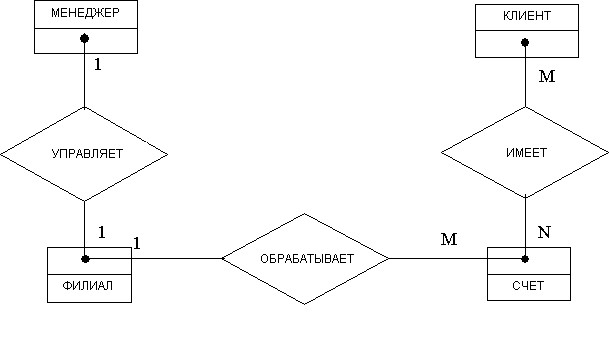
\includegraphics[width=0.8\textwidth]{assets/security/pic25.png}
		\caption{ER-модель предметной области БАНК}
		\label{fig:mesh28}
	\end{figure}
	
	\item \textbf{Определение атрибутов и их документирование.}
	Выявляются все атрибуты, описывающие сущности созданной ER-модели. Каждому атрибуту присваивается осмысленное
	имя, понятное пользователям. О каждом атрибуте в словарь данных помещаются следующие сведения:
	\begin{itemize}
		\item имя атрибута и его описание;
		
		\item тип и размерность значений;
		
		\item значение, принимаемое для атрибута по умолчанию (если такое имеется);
		
		\item может ли атрибут иметь NULL-значения;
		
		\item является ли атрибут составным, и если это так, то из каких простых атрибутов он состоит.
		Например, атрибут <<Ф.И.О. клиента>> может состоять из простых атрибутов <<Фамилия>>, <<Имя>>,
		<<Отчество>>, а может быть простым, содержащим единые значения, как-то <<Сидорский Евгений
		Михайлович>>. Если пользователь не нуждается в доступе к отдельным элементам <<Ф.И.О.>>,
		то атрибут представляется как простой;
		
		\item является ли атрибут расчетным, и если это так, то как вычисляются его значения.
	\end{itemize}
	
	\item \textbf{Определение значений атрибутов и их документирование.}
	Для каждого атрибута сущности, участвующей в ER-модели, определяется набор допустимых значений и ему
	присваивается имя. Например, атрибут <<Тип счета>> может иметь только значения <<депозитный>>, <<текущий>>,
	<<до востребования>>, <<карт-счет>>. Обновляются записи словаря данных, относящиеся к атрибутам, – в них
	заносятся имена наборов значений атрибутов.
	
	\item \textbf{Определение первичных ключей для сущностей и их документирование.}
	На этом шаге руководствуются определением первичного ключа – как атрибута или набора атрибутов сущности,
	позволяющего уникальным образом идентифицировать ее экземпляры. Сведения о первичных ключах помещаются
	в словарь данных.
	
	\item \textbf{Обсуждение концептуальной модели данных с конечными пользователями.}
	Концептуальная модель данных представляется ER-моделью с сопроводительной документацией, содержащей
	описание разработанной модели данных. Если будут обнаружены несоответствия предметной области, то в
	модель вносятся изменения  до тех пор, пока пользователи не подтвердят, что предложенная им модель
	адекватно отображает их личные представления.
\end{enumerate}

\subsubsection{Логическое  проектирование}

Цель этапа логического проектирования – преобразование концептуальной модели на основе выбранной модели данных
в логическую модель, не зависимую от особенностей используемой в дальнейшем СУБД для физической реализации базы
данных. Для ее достижения выполняются следующие процедуры \autocite{oscerko}:
\begin{enumerate}
    \item \textbf{Выбор модели данных.}
        Чаще всего выбирается реляционная модель данных в связи с наглядностью табличного представления данных
        и удобства работы с ними.

    \item \textbf{Определение набора таблиц исходя из ER-модели и их документирование.}
        Для каждой сущности ER-модели создается таблица. Имя сущности – имя таблицы. Причем каждому атрибуту
        сущности соответствует столбец таблицы. Правила генерации таблиц из ER-диаграмм опираются на два основных
        фактора – тип связи и класс принадлежности сущности. Устанавливаются связи между таблицами посредством
        механизма первичных и внешних ключей. Структуры таблиц и установленные связи между ними документируются.

        Изложим правила генерации таблиц из ER-диаграмм, используя пример ER-модели предметной
        области БАНК, представленной на рис. 7, со следующими наборами атрибутов сущностей предметной области БАНК,
        представленными на рис. 8.

    \begin{figure}[H]
        \centering
        \includegraphics[width=0.8\textwidth]{assets/security/pic2.png}
        \caption{Пример ER-модели предметной области БАНК}
        \label{fig:mesh04}
    \end{figure}

    \begin{figure}[H]
        \centering
        \includegraphics[width=0.8\textwidth]{assets/security/pic3.png}
        \caption{Наборы атрибутов сущностей предметной области БАНК}
        \label{fig:mesh05}
    \end{figure}

    Для связи типа 1:1 существуют три отдельных правила формирования предварительных таблиц из ER-диаграмм.

    \underline{Правило 1}

    Если связь типа 1:1 и класс принадлежности обеих сущностей является обязательным, то необходима только одна
    таблица. Первичным ключом этой таблицы может быть первичный ключ любой из двух сущностей.

    На ER-диаграмме связи 1:1, класс принадлежности сущностей МЕНЕДЖЕР, ФИЛИАЛ является обязательным. Тогда согласно
    правилу 1 должна быть сгенерирована одна таблица следующей структуры:

    \begin{figure}[H]
        \centering
        \includegraphics[width=100mm]{assets/security/pic4.png}
        \label{fig:mesh06}
    \end{figure}

    Первичным ключом этой таблицы может быть и первичный ключ сущности МЕНЕДЖЕР – НМ.

    \underline{Правило 2}

    Если связь типа 1:1 и класс принадлежности одной сущности является обязательным, а другой – необязательным,
    то необходимо построить таблицу для каждой сущности. Первичный ключ сущности должен быть первичным ключом
    соответствующей таблицы. Первичный ключ сущности, для которой класс принадлежности является необязательным,
    добавляется как атрибут в таблицу для сущности с обязательным классом принадлежности.

    Представим, что на ER-диаграмме связи 1:1, изображенной на рис. 7, класс принадлежности сущности МЕНЕДЖЕР
    будет обязательный, а сущности ФИЛИАЛ – необязательный. Тогда согласно правилу 2 должны быть сгенерированы
    две таблицы следующей структуры:

    \begin{figure}[H]
        \centering
        \includegraphics[width=100mm]{assets/security/pic5.png}
        \label{fig:mesh07}
    \end{figure}

    Сущность с необязательным классом принадлежности (ФИЛИАЛ) именуется родительской, а с обязательным (МЕНЕДЖЕР)
    – дочерней. Первичный ключ родительской сущности (НФ), помещаемый в таблицу, представляющую дочернюю сущность,
    называется внешним ключом родительской сущности. Связь между указанными таблицами устанавливается путем связи
    первичного и внешнего ключа и имеет вид:

    \begin{figure}[H]
        \centering
        \includegraphics[width=0.8\textwidth]{assets/security/pic6.png}
        \label{fig:mesh08}
    \end{figure}

    Примечание. Если внешний ключ представляет связь 1:1, то должны быть запрещены его дублирующие значения.

    \underline{Правило 3}

    Если связь типа 1:1 и класс принадлежности обеих сущностей является необязательным, то необходимо построить
    три таблицы – по одной для каждой сущности и одну для связи. Первичный ключ сущности должен быть первичным
    ключом соответствующей таблицы. Таблица для связи среди своих атрибутов должна иметь ключи обеих сущностей.

    Представим, что на ER-диаграмме связи 1:1, изображенной на рис. 7, класс принадлежности сущностей МЕНЕДЖЕР,
    ФИЛИАЛ будет необязательный. Тогда согласно правилу 3 должны быть сгенерированы три таблицы следующей структуры:

    \begin{figure}[H]
        \centering
        \includegraphics[width=100mm]{assets/security/pic7.png}
        \label{fig:mesh09}
    \end{figure}

    При этом осуществляется декомпозиция связи 1:1 на две связи 1:1 следующим образом:

    \begin{figure}[H]
        \centering
        \includegraphics[width=0.8\textwidth]{assets/security/pic8.png}
        \label{fig:mesh10}
    \end{figure}

    Для связи типа 1:М существуют только два правила. Выбор одного из них зависит от класса принадлежности
    сущности на стороне M. Класс принадлежности сущности на стороне 1 не влияет на выбор.

    \underline{Правило 4}

    Если связь типа 1:М и класс принадлежности сущности на стороне М является обязательным, то необходимо
    построить таблицу для каждой сущности. Первичный ключ сущности должен быть первичным ключом соответствующей
    таблицы. Первичный ключ сущности на стороне 1 добавляется как атрибут в таблицу для сущности на стороне М.

    На ER-диаграмме связи 1:М, представленной на рис. 7, класс принадлежности сущности СЧЕТ является обязательным.
    Тогда согласно правилу 4 должны быть сгенерированы две таблицы следующей структуры:

    \begin{figure}[H]
        \centering
        \includegraphics[width=100mm]{assets/security/pic9.png}
        \label{fig:mesh11}
    \end{figure}

    Связь между указанными таблицами будет иметь вид:

    \begin{figure}[H]
        \centering
        \includegraphics[width=0.8\textwidth]{assets/security/pic10.png}
        \label{fig:mesh12}
    \end{figure}

    Примечание. Если внешний ключ представляет связь 1:М, то должны быть разрешены его дублирующие значения.

    \underline{Правило 5}

    Если связь типа 1:М и класс принадлежности сущности на стороне М является необязательным,
    то необходимо построить три таблицы – по одной для каждой сущности и одну для связи. Первичный ключ сущности
    должен быть первичным ключом соответствующей таблицы. Таблица для связи среди своих атрибутов должна
    иметь ключи обеих сущностей.

    Представим, что на ER-диаграмме связи 1:М, изображенной на рис. 7, класс принадлежности сущности СЧЕТ
    является необязательным. Тогда согласно правилу 5 должны быть сгенерированы три таблицы следующей структуры:

    \begin{figure}[H]
        \centering
        \includegraphics[width=100mm]{assets/security/pic11.png}
        \label{fig:mesh13}
    \end{figure}

    При этом осуществляется декомпозиция связи 1:М на две связи – 1:М и 1:1 – следующим образом

    \begin{figure}[H]
        \centering
        \includegraphics[width=0.8\textwidth]{assets/security/pic12.png}
        \label{fig:mesh14}
    \end{figure}

    Для связи типа М:N класс принадлежности сущности не имеет значения.

    \underline{Правило 6}

    Если связь типа М:N, то необходимо построить три таблицы – по одной для каждой сущности и одну для связи.
    Первичный ключ сущности должен быть первичным ключом соответствующей таблицы. Таблица для связи среди своих
    атрибутов должна иметь ключи обеих сущностей.

    ER-диаграмма связи М:N имеется на рис. 7. Согласно правилу 6 на основе этой ER-диаграммы должны быть
    сгенерированы три таблицы следующей структуры:

    \begin{figure}[H]
        \centering
        \includegraphics[width=100mm]{assets/security/pic13.png}
        \label{fig:mesh15}
    \end{figure}

    При этом осуществляется декомпозиция связи М:N на две связи 1:М следующим образом:

    \begin{figure}[H]
        \centering
        \includegraphics[width=0.8\textwidth]{assets/security/pic14.png}
        \label{fig:mesh16}
    \end{figure}

    В таблице КЛИЕНТ–СЧЕТ клиенту, имеющему, например, три счета будут соответствовать три строки
    с одним и тем же номером клиента. А счет, у которого, например, два владельца, представляется двумя
    строками с различными номерами клиентов, владеющими этим счетом.

    К ER-модели предметной области БАНК, представленной на рис. 7, применимы правила 1, 4, 6. Связь МЕНЕДЖЕР
    – ФИЛИАЛ представляется (согласно правилу 1) одной таблицей А:

    \begin{figure}[H]
        \centering
        \includegraphics[width=0.8\textwidth]{assets/security/pic15.png}
        \label{fig:mesh17}
    \end{figure}

    Связь ФИЛИАЛ – СЧЕТ  представляется (согласно правилу 4) связью:

    \begin{figure}[H]
        \centering
        \includegraphics[width=0.8\textwidth]{assets/security/pic16.png}
        \label{fig:mesh18}
    \end{figure}

    Связь КЛИЕНТ – СЧЕТ представляется (согласно правилу 6) связью:

    \begin{figure}[H]
        \centering
        \includegraphics[width=0.8\textwidth]{assets/security/pic17.png}
        \label{fig:mesh19}
    \end{figure}

    Анализ состава атрибутов полученных таблиц A, B, C, D, E, F показывает, что таблица В является составной
    частью таблицы А, таблица Е – составной частью таблицы С. Поэтому таблицы В, Е можно исключить из рассмотрения.
    Оставшиеся таблицы А, С, D, F можно связать посредством связи первичных и внешних ключей.
    В результате получим реляционную модель для ER-модели предметной области БАНК.

    \item \textbf{Нормализация таблиц.}
        Для правильного выполнения нормализации проектировщик должен глубоко изучить семантику и особенности
        использования данных. На этом шаге он проверяет корректность структуры таблиц, созданных на предыдущем
        шаге, посредством применения к ним процедуры нормализации. Она заключается в приведении каждой из таблиц,
        по крайней мере, к 3НФ. В результате нормализации получается очень гибкий проект базы данных,
        позволяющий легко вносить в нее нужные расширения.

        Нормализация таблиц - процесс, позволяющий минимизировать избыточность данных. Чтобы пояснить этот процесс,
        будем исходить из описания предметной области БАНК, представленного на рис. 7, и предположения, что на его
        основе была разработана база данных, состоящая из следующих двух таблиц:

    \begin{figure}[H]
        \centering
        \includegraphics[width=0.8\textwidth]{assets/security/pic18.png}
        \label{fig:mesh20}
    \end{figure}

    \underline{1 нормальная форма (1НФ)}

    Таблица находится в 1НФ, если все ее поля содержат только простые неделимые значения.

    Таблицы ФИЛИАЛ и КЛИЕНТ не удовлетворяют требованиям 1НФ. Для приведения их к 1НФ в них надо вставить новые
    записи следующим образом:

    \begin{figure}[H]
        \centering
        \includegraphics[width=0.8\textwidth]{assets/security/pic19.png}
        \label{fig:mesh21}
    \end{figure}

    Но полученные таблицы неэффективны, так как содержат много избыточной информации. Необходимо их привести к 2НФ.

    \underline{2 нормальная форма (2НФ)}

    Таблица находится в 2НФ, если она удовлетворяет требованиям 1НФ и неключевые поля функционально полно
    зависят от первичного ключа.

    Функциональная зависимость – это понятие, отображающее определенную семантическую связь между полями таблицы.
    Неключевое поле А функционально полно зависит от первичного ключа, если:
    \begin{enumerate}
        \item оно функционально зависит от первичного ключа, т.е. каждой комбинации значений полей первичного
        ключа соответствует одно и только одно значение поля А;

        \item не существует функциональной зависимости А ни от какого подмножества полей первичного ключа
        (в противном случае А находится в частичной функциональной зависимости от первичного ключа).
    \end{enumerate}

    В таблице КЛИЕНТ неключевые поля ФИО\_К, СОЦ\_П, АДР\_К функционально зависят от ключа (НК, НС). Кроме того,
    они функционально зависят от подмножества ключа – НК. Следовательно, неключевые поля ФИО\_К, СОЦ\_П, АДР\_К
    находятся в частичной функциональной зависимости от первичного ключа (НК, НС) и нарушаются требования 2НФ.
    Эти поля надо из таблицы КЛИЕНТ удалить. Полученную в результате этого таблицу назовем КЛИЕНТ–СЧЕТ, которая
    имеет вид:

    \begin{figure}[H]
        \centering
        \includegraphics[width=40mm]{assets/security/pic20.png}
        \label{fig:mesh22}
    \end{figure}

    Эта таблица удовлетворяет требованиям 2НФ.

    Удаленные неключевые поля помещаются в новую таблицу совместно с подмножеством НК, от которого они зависят.
    И это подмножество будет первичным ключом новой таблицы КЛИЕНТ вида:

    \begin{figure}[H]
        \centering
        \includegraphics[width=0.8\textwidth]{assets/security/pic21.png}
        \label{fig:mesh23}
    \end{figure}

    Новая таблица КЛИЕНТ также удовлетворяет требованиям 2НФ. Ее неключевые поля функционально полно зависят
    от первичного ключа.

    Полученные таблицы не содержат избыточной информации, и нет основания приводить их к 3НФ. Таблица ФИЛИАЛ
    удовлетворяет требованиям 2НФ, так как ее неключевые поля НФ, АДР\_Ф, НМ, ОСТ, ТИП функционально полно
    зависят от первичного ключа. Но в таблице ФИЛИАЛ повторяется информация о филиале для всех счетов,
    обрабатываемых им. Поэтому ее надо привести к 3НФ.

    \underline{3 нормальная форма (3НФ)}

    Таблица находится в 3НФ, если она удовлетворяет требованиям 2НФ и не содержит транзитивных зависимостей.

    Транзитивной зависимостью называется функциональная зависимость между неключевыми полями. В таблице ФИЛИАЛ
    она наблюдается. Следовательно, нарушаются требования 3НФ. Из таблицы ФИЛИАЛ надо удалить поля, участвующие
    в этой транзитивной зависимости, – АДР\_Ф, НМ. Получится таблица, характеризующая счет, вида:

    \begin{figure}[H]
        \centering
        \includegraphics[width=100mm]{assets/security/pic22.png}
        \label{fig:mesh24}
    \end{figure}

    Затем создается новая таблица, в которую помещаются удаленные поля и поле, от которого они зависят. Она имеет вид:

    \begin{figure}[H]
        \centering
        \includegraphics[width=100mm]{assets/security/pic23.png}
        \label{fig:mesh25}
    \end{figure}

    Полученные таблицы приведены к 3НФ. В них каждая запись есть отдельное независимое утверждение. Повторяются
    только значения внешнего ключа НФ в таблице СЧЕТ, что неизбежно, так как одним филиалом могут обрабатываться
    несколько счетов.

    Как видим, нормализация приводит к фрагментации исходных таблиц. В нашем примере таблица КЛИЕНТ разбивается
    на таблицы 1, 2, а таблица ФИЛИАЛ  – на таблицы 3, 4. Осуществив связь этих таблиц посредством связи первичных
    и внешних ключей, получим реляционную модель данных предметной области БАНК, в которой минимизирована
    избыточность данных:

    \begin{figure}[H]
        \centering
        \includegraphics[width=0.8\textwidth]{assets/security/pic24.png}
        \label{fig:mesh26}
    \end{figure}

    \item \textbf{Проверка логической модели данных на предмет возможности выполнения всех транзакций, предусмотренных пользователями.}
        Транзакция – это набор действий, выполняемых отдельным пользователем или прикладной программой с целью
        изменения содержимого базы данных. Так, примером транзакции в проекте БАНК может быть передача права
        распоряжаться счетами некоторого клиента другому клиенту. В этом случае в базу данных потребуется внести
        сразу несколько изменений. Если во время выполнения транзакции произойдет сбой в работе компьютера,
        то база данных окажется в противоречивом состоянии, так как некоторые изменения уже будут внесены, а
        остальные еще нет. Поэтому все частичные изменения должны быть отменены для возвращения базы данных в
        прежнее непротиворечивое состояние.

        Перечень транзакций определяется действиями пользователей в предметной области. Используя ER-модель,
        словарь данных и установленные связи между первичными и внешними ключами, производится попытка выполнить
        все необходимые операции доступа к данным вручную. Если какую-либо операцию выполнить вручную не удается,
        то составленная логическая модель данных является неадекватной и содержит ошибки, которые надо устранить.
        Возможно, они связаны с пропуском в модели сущности, связи или атрибута.

    \item \textbf{Определение требований поддержки целостности данных и их документирование.}
        Эти требования представляют собой ограничения, которые вводятся с целью предотвратить помещение в базу
        данных противоречивых данных. На этом шаге вопросы целостности данных освещаются безотносительно к
        конкретным аспектам ее реализации. Должны быть рассмотрены следующие типы ограничений:
        \begin{itemize}
            \item обязательные данные. Выясняется, есть ли атрибуты, которые не могут иметь Null-значений;

            \item ограничения для значений атрибутов. Определяются допустимые значения для атрибутов;

            \item целостность сущностей. Она достигается, если первичный ключ сущности не содержит Null-значений;

            \item ссылочная целостность. Она понимается так, что значение внешнего ключа должно обязательно
            присутствовать в первичном ключе одной из строк таблицы для родительской сущности;

            \item ограничения, накладываемые бизнес-правилами. Например, в случае с проектом БАНК может быть
            принято правило, запрещающее клиенту распоряжаться, скажем, более чем тремя счетами.
        \end{itemize}

    Сведения обо всех установленных ограничениях целостности данных помещаются в словарь данных.

    \item \textbf{Создание окончательного варианта логической модели данных и обсуждение его с пользователями.}
        На этом шаге подготавливается окончательный вариант ER-модели, представляющей логическую модель данных.
        Сама модель и обновленная документация, включая словарь данных и реляционную схему связи таблиц,
        представляется для просмотра и анализа пользователям, которые должны убедиться, что она точно
        отражает предметную область.
\end{enumerate}

\subsubsection{Физическое проектирование}

Цель этапа физического проектирования – описание конкретной реализации базы данных, размещаемой во внешней
памяти компьютера. Это описание структуры хранения данных и эффективных методов доступа к данным базы. При
логическом проектировании отвечают на вопрос – что надо сделать, а при физическом – выбирается способ, как
это сделать. Процедуры физического проектирования следующие \autocite{oscerko}:
\begin{enumerate}
    \item \textbf{Проектирование таблиц базы данных средствами выбранной СУБД.}
        Осуществляется выбор реляционной СУБД, которая будет использоваться для создания базы данных,
        размещаемой на машинных носителях. Глубоко изучаются ее функциональные возможности по проектированию
        таблиц. Затем выполняется проектирование таблиц и схемы их связи в среде СУБД. Подготовленный проект
        базы данных описывается в сопроводительной документации.

    \item \textbf{Реализация бизнес-правил в среде выбранной СУБД.}
        Обновление информации в таблицах может быть ограничено бизнес-правилами. Способ их реализации
        зависит от выбранной СУБД. Одни системы для реализации требований предметной области предлагают
        больше возможностей, другие – меньше. В некоторых системах вообще отсутствует поддержка реализации
        бизнес-правил. В таком случае разрабатываются приложения для реализации их ограничений. Все решения,
        принятые в связи с реализацией бизнес-правил предметной области, подробно описываются в сопроводительной
        документации.

    \item \textbf{Проектирование физической организации базы данных.}
        На этом шаге выбирается наилучшая файловая организация для таблиц. 
        
        Выполняется \textbf{проектирование транзакций} \autocite{koch}:
        
        Цель проектирования транзакций заключается в определении и
        документировании высокоуровневых характеристик всех транзакций,
        которые должны будут выполняться в разрабатываемой базе данных. Эту
        работу следует выполнить еще на начальной стадии проектирования, что
        позволит обеспечить поддержку всех требуемых транзакций со стороны
        логической модели данных. При этом очень важно, чтобы характеристики
        всех транзакций были зафиксированы в документации. Существует
        несколько методов описания высокоуровневых характеристик транзакций.
        Наиболее важные из них следующие:
        
        \begin{itemize}
        	\item данные, которые используются транзакцией;
        
        	\item функциональные характеристики транзакции;
        
        	\item выходные данные, формируемые транзакцией;
        
        	\item степень важности транзакции для пользователей;
        
        	\item предполагаемая интенсивность использования. 
        \end{itemize}
        	
        Для того чтобы разрабатываемый физический проект базы данных
        обладал требуемым уровнем эффективности, необходимо получить
        максимум сведений о тех транзакциях, которые будут выполняться в
        проектируемой базе данных. Для этого потребуются как качественные, так и
        количественные характеристики. Для каждой транзакции необходимо знать
        следующее:
        
        \begin{itemize}
        	\item транзакции, выполняемые наиболее часто и оказывающие
        	существенное влияние на производительность;
        
        	\item транзакции, наиболее важные для работы организации;
        
        	\item периоды времени на протяжении суток/недель, в которые нагрузка
       		базы данных возрастает до максимума (называемые периодами пиковой
        	нагрузки);
        
        	\item ожидаемая частота выполнения транзакций;
        
        	\item отношения и атрибуты, к которым потребуется иметь доступ при
       		выполнении транзакции, а также тип этого доступа;
        
        	\item ограничения, устанавливаемые на время выполнения транзакций.
        \end{itemize} 
        
        На основании указанных показателей принимаются решения об оптимизации производительности базы данных путем определения индексов
        в таблицах, ускоряющих выборку данных из базы, или снижения требований к уровню нормализации таблиц.
        Проводится оценка дискового объема памяти, необходимого для размещения создаваемой базы данных.
        Стремятся к его минимизации. Принятые решения по изложенным вопросам документируются.
        
		При этом стоит понимать, что индексы занимают место в БД. При вводе новых данных или удалении
		данных СУБД приходится обновлять и таблицы, и индексы. Это может
		замедлить выполнение операций модификации данных, особенно для таблиц
		с большим числом строк, как в хранилище данных. Таким образом, может появиться
		проблема, суть которой состоит в возникновении конфликта между
		скоростью обновления данных в таблице и скоростью ее считываний. При
		разрешении этой проблемы следует придерживаться следующего
		эмпирического правила: создавать индексы для колонок первичных ключей и
		других колонок, часто используемых в тех запросах, в которых для выборки
		данных применяются логические критерии. Если в результате скорость
		обновления данных ухудшается, то можно рассмотреть вопрос об удалении
		некоторых индексов.
        
    \item \textbf{Разработка стратегии защиты базы данных.}
        База данных представляет собой ценный корпоративный ресурс, и организации ее защиты уделяется большое
        внимание. Для этого проектировщики должны иметь полное и ясное представление обо всех средствах защиты,
        предоставляемых выбранной СУБД.

    \item \textbf{Организация мониторинга функционирования базы данных и ее настройка.}
        После создания физического проекта базы данных организуется непрерывное слежение за ее функционированием.
        Полученные сведения об уровне производительности базы данных используются для ее настройки. Для этого
        привлекаются и средства выбранной СУБД.
\end{enumerate}

Решения о внесении любых изменений в функционирующую базу данных должны быть обдуманными и всесторонне взвешенными.

\subsubsection{Особенности проектирования OLAP и OLTP систем}

СУБД, созданная для поддержки оперативной обработки транзакций,
называется \textbf{OLTP-системой} (Online Transaction Processing). \textbf{OLAP} (online analytical processing) обычно подразумевает запрос этих транзакций в базе данных для аналитических целей. 

В таблице ниже представлено сравнение систем OLTP и OLAP\autocite{oracle_OLTP}.

\begin{table}[!ht]
	\centering
	\begin{tabular}{|m{4cm}|m{6cm}|m{6cm}|}
		\hline
		 ~ &\textbf{OLTP-системы} & \textbf{OLAP-системы} \\ 
		\hline
		Цель & Основная цель OLTP-систем — обработка текущих транзакций в реальном времени. Эти системы используются для оперативной обработки данных, таких как обработка заказов, банковские транзакции, управление запасами и т.д. & Основная цель OLAP-систем — анализ данных для поддержки принятия решений. Эти системы используются для выполнения сложных запросов и анализа больших объемов данных, таких как отчеты по продажам, финансовый анализ, маркетинговые исследования и т.д. \\ 
		\hline
		Структура данных & Данные в OLTP-системах обычно нормализованы, чтобы избежать избыточности и обеспечить целостность данных. Это означает, что данные разбиты на множество таблиц с минимальной избыточностью. & Данные в OLAP-системах обычно денормализованы и хранятся в виде многомерных структур (например, кубов данных). Это позволяет быстро выполнять сложные запросы и агрегации. \\ 
		\hline
		Объем данных & Обрабатывает относительно небольшие объемы данных за одну транзакцию, но может обрабатывать большое количество транзакций в единицу времени. & Обрабатывает большие объемы данных, которые могут включать исторические данные за длительные периоды времени.\\ 
		\hline
		Типы запросов &  Запросы обычно простые и часто повторяющиеся, такие как вставка, обновление, удаление и простые выборки данных. &Запросы обычно сложные и уникальные, включающие агрегации, фильтрацию, сортировку и другие операции анализа данных. \\ 
		\hline
		Хранение данных &  Данные хранятся в реляционных базах данных, таких как MySQL, PostgreSQL, Oracle и другие. & Данные могут храниться в специализированных хранилищах данных (data warehouses) или в многомерных базах данных (OLAP-кубы).\\ 
		\hline
	\end{tabular}
\end{table}

Эти различия подчеркивают, что OLTP и OLAP-системы предназначены для разных задач и требуют разных подходов к проектированию и оптимизации.

Проектирование информационных систем для OLTP и OLAP требует учета различных профилей нагрузки, чтобы обеспечить оптимальную производительность и надежность. Рассмотрим различные профили нагрузки и их влияние на проектирование OLTP и OLAP систем \autocite{OLAP_OLTP}.


\textbf{Профили нагрузки для OLTP систем}:
\begin{itemize}
	\item Высокая частота транзакций:

	Описание: Большое количество транзакций в секунду (TPS).

	Проектирование: Использование высокопроизводительных баз данных, оптимизация индексов, кэширование данных, горизонтальное масштабирование (sharding).

	\item Низкая латентность:

	Описание: Требование минимального времени отклика на транзакции.
	
	Проектирование: Оптимизация запросов, использование внутренней памяти для хранения часто используемых данных, минимизация блокировок.
	
	\item Высокая доступность:

	Описание: Система должна быть доступна 24/7.
	
	Проектирование: Репликация данных, кластеризация, автоматическое восстановление после сбоев, резервное копирование.
	
	\item Целостность данных:

	Описание: Обеспечение точности и согласованности данных.
	
	Проектирование: Использование транзакций с ACID-свойствами, валидация данных, аудит и логирование изменений.
\end{itemize}

\textbf{Профили нагрузки для OLAP систем}:

\begin{itemize}
	
	\item Сложные аналитические запросы:

	Описание: Выполнение сложных запросов с агрегацией, фильтрацией и сортировкой.
	
	Проектирование: Оптимизация запросов, использование многомерных структур данных (OLAP-кубы), предварительная агрегация данных.
	
	\item Высокий объем данных:

	Описание: Обработка больших объемов данных.
	
	Проектирование: Использование хранилищ данных (data warehouses), горизонтальное масштабирование, распределенные вычисления.
	
	\item Исторические данные:

	Описание: Хранение и анализ данных за длительные периоды времени.
	
	Проектирование: Эффективное управление версиями данных, архивирование, использование временных баз данных.
	
	\item Высокая скорость отклика на запросы:

	Описание: Требование быстрого выполнения аналитических запросов.
	
	Проектирование: Оптимизация индексов, кэширование результатов запросов, использование материализованных представлений.
\end{itemize}

Проектирование информационных систем для OLTP и OLAP требует учета различных профилей нагрузки, чтобы обеспечить оптимальную производительность и надежность. OLTP-системы оптимизированы для высокой частоты транзакций и низкой латентности, тогда как OLAP-системы оптимизированы для выполнения сложных аналитических запросов и обработки больших объемов данных. Понимание этих различий позволяет разработчикам и архитекторам создавать системы, которые эффективно справляются с соответствующими нагрузками.

\subsection{Формальные верификации и спецификации}
Информация взята из \autocite{Glukharev}

Оценивание качества программного обеспечения информационных систем неразрывно связано с процессом верификации,
т. е. с подтверждением того, что функциональные возможности ПО соответствуют их описаниям в программной документации
(т.е. их спецификации). Функциональные возможности, которые не имеют описания в документации или не соответствуют
описанию, называются недекларированными возможностями. Они могут являться как следствием ошибок разработчика,
так и результатом выполнения умышленно внедрённого в программу кода. Как случайные, так и преднамеренные НДВ
(последние называются также программными закладками) представляют угрозу информационной безопасности программных
систем. Цель верификации программ – выявление и регистрация НДВ для последующего их устранения.

Любое программное средство обладает определённой корректностью. Понятие корректность является более узким,
чем понятие качество, так как последнее включает в себя такие характеристики, как надёжность, мобильность,
понятность, сопровождаемость программной системы. Корректность характеризует функциональные возможности программы,
т. е. одну из составляющих качества. Корректность программы наиболее полно определяется степенью её соответствия
программной спецификации.

В настоящее время существует множество методов и средств автоматизированной верификации ПО, часто применяемых
совместно, взаимно дополняющих друг друга. Но не менее важным, чем ПО, компонентом ИС является база данных.
Она также оказывает влияние на качество ИС и нуждается в верификации. Для проведения полноценной
верификации требуется:
\begin{itemize}
    \item правильное понимание сущности БД;

    \item система количественных и качественных показателей корректности БД;

    \item наличие автоматизированных систем верификации БД.
\end{itemize}

На современном этапе БД должны рассматриваться не только как хранилища данных, но и как полноценные программные
компоненты. Обоснованием данного положения служит практика использования промышленных СУБД и ИС, основанная
в значительной степени на использовании клиент-серверной архитектуры и технологии активного сервера. Суть последней
заключается в том, что функции ИС, выполняющие обработку данных в БД, реализуются не в клиентских приложениях, а
на стороне сервера СУБД в виде хранимых подпрограмм БД. Слово «хранимый» указывает на то, что коды этих подпрограмм
располагаются вместе с данными и являются, таким образом, объектами БД.

Известно три типа хранимых подпрограмм: функции, процедуры и триггеры.

Функции и процедуры запускаются на выполнение путём явного вызова. Клиентскому приложению, чтобы вызвать процедуру,
необходимо предварительно соединиться с БД, где расположен ее откомпилированный код. Обращение к процедуре
производится по имени с передачей входных данных и, возможно, с заданием выходных параметров. Функция отличается
от процедуры тем, что она всегда возвращает атомарное значение определённого типа и вызывается путем использования
в арифметических и логических выражениях на месте операнда.

Триггер – это специальный тип хранимых подпрограмм. Он выполняется автоматически в ответ на вставку, обновление
или удаление записей в таблице и служит для поддержания корректности и согласованности (целостности) данных.
Реализация хранимых подпрограмм возможна как на языке баз данных, так и на языках программирования высокого уровня
C, C++, Pascal, Java.

Из сказанного следует, что БД, поддерживаемые промышленными СУБД имеют двойственную природу. Оставаясь хранилищами
данных, они одновременно играют роль программного обеспечения в ИС или, точнее, становятся полноценными программными
компонентами, напоминающими динамически подключаемые библиотеки операционной системы Windows или COM-объекты.
Как и любая другая часть ИС, БД нуждаются в верификации и тестировании.

Учитывая то, что верификация есть подтверждение корректности, необходимо заметить, что корректность БД
должна оцениваться при помощи системы математических показателей. К числу наиболее часто встречающихся сегодня на
практике функциональных показателей корректности БД относятся следующие:
\begin{itemize}
    \item \textbf{полнота накопленных описаний объектов} – относительное число объектов и документов, имеющихся
    в БД, к общему числу объектов в аналогичной БД;

    \item \textbf{достоверность} – степень соответствия записей БД реальным объектам в данный момент времени;

    \item \textbf{идентичность данных} – относительное число описаний объектов, не содержащих ошибки,
    к общему числу документов об объектах в БД;

    \item \textbf{актуальность данных} – относительное число устаревших данных к общему числу накопленных
    и обрабатываемых записей.
\end{itemize}

Помимо функциональных показателей, существуют конструктивные показатели корректности, отличающиеся большей
универсальностью, независимостью от сферы применения базы данных:
\begin{itemize}
    \item \textbf{объем БД} – число описаний объектов или документов в БД, доступных для хранения и обработки;

    \item \textbf{оперативность} – степень соответствия динамики изменения данных в процессе сбора и обработки
    состояниям реальных объектов, или величина запаздывания между появлением (изменением) характеристик
    реального объекта и его отражением в БД;

    \item \textbf{периодичность} – промежуток времени между поставками двух последовательных, достаточно
    различающихся информацией версий БД;

    \item \textbf{глубина ретроспективы} – интервал времени от даты выпуска (записи в БД) самого раннего
    документа до настоящего времени;

    \item \textbf{динамичность} – относительное число изменяемых описаний объектов к общему числу записей в
    БД за некоторый интервал времени, определяемый периодичностью издания версий БД.
\end{itemize}

Оценивание корректности БД предполагает анализ ее содержимого, логической структуры и программной составляющей
(хранимых подпрограмм). В связи с этим необходимо различать три вида корректности БД: корректность содержимого,
корректность схемы данных и программная корректность. Рассмотрим каждый из перечисленных видов по отдельности.

\textbf{Корректность содержимого.} Любая запись в БД должна адекватно отражать характеристики реального
существующего объекта, экземпляра сущности предметной области; если же в записи фиксируется информация
о взаимодействии объектов, то речь должна идти о взаимодействии, имеющем место в реальной действительности.

Очевидно, что корректность содержимого определяется функциональными и конструктивными показателями,
рассмотренными выше.

\textbf{Корректность схемы данных.} Традиционно под реляционной схемой понимается набор взаимосвязанных схем
отношений или, с точки зрения обычного пользователя, весь набор таблиц БД. Можно выделить следующие подвиды
корректности схемы данных:

\begin{enumerate}
    \item \textbf{Точность отображения концептуальной схемы (ER-схемы) на реляционную.}

        Концептуальная модель реляционной БД обычно представляется в виде диаграмм сущность–связь, или ER-диаграмм,
        на которых показываются объекты предметной области и связи (способы взаимодействия) между ними. При
        концептуальном проектировании не оперируют понятиями «таблица», «внешний ключ» и т. п. Но ER-диаграммы
        легко преобразуются в схему реляционной БД по набору типовых правил. В итоге сущностям, представленным на ER-схеме,
        соответствуют таблицы реляционной БД, а связям – вспомогательные таблицы и внешние ключи. Типовые правила
        отображения дают возможность «обратного проектирования» – получения ER-схемы по имеющейся реляционной схеме БД.
        Однако не всегда «обратное проектирование» даёт ER-схему, эквивалентную исходной концептуальной модели.
        Причиной этого в ряде случаев является неточность прямого преобразования, в результате чего схема БД получается
        некорректной по отношению к исходной ER-модели.

        Точность отображения, очевидно, может быть определена как соответствие ER-схемы, полученной в результате
        «обратного проектирования», исходной концептуальной схеме. Точность отображения характеризуется множеством
        показателей, учитывающих детализацию сравнения на уровне атрибутов, сущностей, связей и участков ER-диаграмм,
        образованных двумя отдельно взятыми сущностями и одной ассоциацией между ними.

        В каждом случае необходимо рассчитывать относительное число правильно отображенных на реляционную схему
        сущностей, атрибутов, связей и участков, к общему числу соответствующих элементов, определенных на этапе
        концептуального проектирования. С другой стороны, в процессе создания реляционной схемы могут появиться
        недекларированные атрибуты, сущности и связи. Процесс верификации БД должен включать в себя оценивание их
        процентного содержания в общем числе отраженных на реляционной схеме сущностей, атрибутов и связей
        соответственно. Чем ниже процентное содержание недекларированных элементов схемы данных, тем корректнее БД
        по отношению к концептуальной модели.

    \item \textbf{Нормализованность таблиц.}

        Основная цель проектирования БД – группирование атрибутов по таблицам так, чтобы минимизировать избыточность
        данных и по возможности сократить объём памяти, необходимый для физического хранения таблиц. Теория нормальных
        форм и нормализации описывает один из формальных методов проектирования БД, в котором идентификация таблиц
        основана на выявлении первичных ключей и функциональных зависимостей между атрибутами.

        Высшей нормальной формой на практике оказывается, как правило, нормальная форма Бойса–Кодда. Согласно её
        требованиям, все неключевые атрибуты таблицы должны полностью функционально зависеть от потенциального ключа,
        а функциональных зависимостей между различными неключевыми атрибутами быть не должно. Нарушение этих
        требований приводит к избыточности данных и, как следствие, к аномалиям вставки, обновления и удаления записей.

        Современные методы проектирования (в том числе упомянутый ранее метод ER-моделирования) позволяют
        автоматически приводить таблицы БД к нормальной форме Бойса–Кодда. Однако ошибки могут возникать, особенно
        если разработчиками принимается нешаблонное решение о частичной денормализации таблиц.

        Проще всего оценивать нормализованность БД при помощи относительного числа полностью нормализованных таблиц
        к общему числу таблиц. Более сложной задачей является оценивание степени допустимости денормализации для
        данного проекта, если таковая имеет место.

    \item \textbf{Логическая целостность.}

        Важной составляющей корректности схемы данных является логическая целостность. С каждой предметной
        областью связаны определённые требования целостности, которые тем или иным образом ограничивают
        диапазоны возможных значений атрибутов сущностей и связей, говорят о допустимости либо недопустимости
        комбинаций некоторых значений. Реализация требований целостности в БД позволяет избавиться от появления
        отрицательных возрастов и масс, от повторения одного и того же ИНН у различных лиц, от некорректной
        последовательности дат начала и завершения работы (в случае, когда они в результате ошибки пользователя
        меняются местами) – словом, избежать появления логически противоречивой, несогласованной, «невозможной»
        с позиции здравого смысла информации.

        Простые требования целостности реализуются при помощи специальных объектов БД, называемых ограничениями.
        Большинством реляционных СУБД сегодня поддерживаются такие ограничения целостности, как первичный ключ,
        внешний ключ, уникальность значений, запрет неопределённых значений и ограничение на основе логического
        условия. Более сложные требования целостности реализуются процедурно с помощью специальных подпрограмм
        – триггеров. Следует заметить, что целостность в данном случае пересекается с программной корректностью,
        которая будет рассматриваться далее. И в первом, и во втором случае речь идёт об автоматическом
        поддержании целостности. Во время выполнения операций вставки, удаления и обновления неверные данные либо
        не принимаются совсем, либо автоматически корректируются.

        Целесообразно оценивать логическую целостность БД при помощи следующих показателей.
        \begin{itemize}
            \item \textbf{Полнота реализации требований целостности} – отношение реализованных в БД ограничений
            и триггеров к общему числу заявленных требований. Ограничения, которые не были заявлены в документации,
            не рассматриваются.

            \item \textbf{Относительное число не заявленных в документации ограничений целостности к общему числу реализованных.}
            Если недекларированных ограничений нет, показатель принимает нулевое значение, что говорит о
            корректности схемы данных.

            \item \textbf{Согласованность ограничений с содержимым таблиц.} Возможны ситуации, когда дополнительное
            ограничение целостности или новый триггер добавляются в уже заполненную БД. При этом нельзя допустить,
            чтобы новое ограничение вошло в противоречие с уже добавленными в таблицы записями. Для обычных
            ограничений целостности эта проблема решена на уровне СУБД. Система запрещает вводить ограничение,
            если в БД уже имеются строки таблиц, которые ему не удовлетворяют. Но СУБД не в состоянии выполнить
            подобную проверку для триггера. Поэтому возможны противоречия: с одной стороны, имеется сложное
            ограничение целостности, реализуемое триггером; с другой стороны, записи, появившиеся в БД до создания
            триггера, могут заведомо не удовлетворять этому ограничению.

            Показатель согласованности ограничений и содержимого таблиц рассчитывается как отношение записей,
            удовлетворяющих всем ограничениям, к общему числу записей. Расчет этого показателя неразрывно связан
            с анализом программного кода триггеров, цель которого – выяснить декларативный смысл каждого триггера.
            Задача эта сама по себе нетривиальна и требует отдельного рассмотрения.

            \item \textbf{Непротиворечивость ограничений.} В результате ошибок проектирования в БД могут возникать
            конфликты между ограничениями и триггерами. Когда разные триггеры и ограничения предъявляют к данным
            противоречивые требования, вплоть до взаимоисключающих, таблицы БД могут оказаться недоступными для
            вставки и обновления строк.

            Свойство непротиворечивости ограничений затруднительно оценить количественно. Вероятно, речь должна
            идти о качественном показателе или комплексе количественных и качественных показателей, позволяющих
            оценить степень изолированности самих ограничений друг от друга, степень доступности данных, с которыми
            связано множество ограничений и триггеров, а также долю противоречивых ограничений во всей БД.

            \item \textbf{Сложность реализации требования целостности.} Даже простые ограничения могут быть
            реализованы с помощью триггеров. Теоретически это допустимо, но на практике подобные решения
            снижают эффективность системы. Кроме того, очевидно, что они затрудняют последующую верификацию
            БД, увеличивают время анализа, так как приходится восстанавливать декларативный смысл каждого
            триггера. Декларативный смысл обычного ограничения целостности всегда ясен из его описания.

            Сложность реализации требования целостности – качественный показатель, оцениваемый для каждого
            триггера. Если данное требование может быть полностью реализовано при помощи стандартных ограничений,
            сложность является очень высокой. В противном случае вычисление показателя производится на основе
            семантического анализа команд, выполняемых в теле триггера. Возможные значения показателя сложности
            реализации: «очень низкая», «низкая», «средняя», «высокая», «очень высокая».
        \end{itemize}
    \item \textbf{Программная корректность баз данных.}

    Корректность программных процедур существенно зависит от их топологической и информационной сложности:
    чем выше сложность, тем больше вероятность появления неумышленных НДВ, с одной стороны, и тем сильнее усложняется
    обнаружение любых НДВ, с другой стороны.

    К настоящему времени предложено множество метрик оценивания сложности программ. Оценивание сложности
    хранимых подпрограмм БД может производиться с использованием метрик размера программ и метрик сложности
    потока управления.

    Исходя из сказанного, можно определить следующие характеристики программной сложности БД:
    \begin{itemize}
        \item \textbf{Суммарная сложность подпрограмм БД.} Вычисляется как алгебраическая сумма сложностей
        (весов) всех подпрограмм. С тем, какой именно показатель (из перечисленных выше) будет характеризовать
        сложность отдельно взятой подпрограммы, необходимо определиться заранее, до выполнения вычислений.

        \item \textbf{Группа показателей, отражающая наличие сцепления между подпрограммами.} Сцепление подпрограмм
        имеет место в том случае, если они используют общие атрибуты таблиц. Малое сцепление в программном
        классе или компоненте желательно, поскольку оно увеличивает инкапсуляцию и снижает вероятность возникновения
        ошибок в поведении компонента. Наиболее простым показателем сцепления является разность между числом пар
        несцепленных и числом пар сцепленных подпрограмм. Отрицательный показатель сцепления всегда приравнивается
        к нулю.
    \end{itemize}
\end{enumerate}

% \input{part/ref}
\newpage
\printbibliography
\end{document}
